% !TeX program = xelatex
\AddToHook{package/projlib-language/before}{\RequirePackage{fvextra}}
\documentclass[11pt,a4paper,oneside,plain,CN,colored-proof=false,
  load-custom-latin-font-file=pku-font-latin.tex,
  load-custom-math-font-file=pku-font-math.tex,
  load-custom-cjk-font-file=pku-font-cjk.tex]{einfart}
% 学习总笔记：公共配置见 ../common/zbstyle.tex。
\newcommand{\PKUDocumentType}{notes}
\newcommand{\PKUCodePalette}{ide}
\newcommand{\PKUShortTitle}{广义线性模型}
\newcommand{\PKUSubtitle}{公共卫生统计 · 学习总笔记}
\newcommand{\PKUVersion}{2.0}

\usepackage{pku-notes}
% 公卫统计 · Einfart/plain 学习总笔记兼容层
% 视觉设置集中于本文件和 pku-notes.sty；原章节、题号、标签保持不变。
\usepackage{multirow,calc,tikz,pgfplots,placeins,pdflscape,microtype}
\usetikzlibrary{arrows.meta,positioning,calc,patterns,decorations.pathreplacing,shapes.geometric}
\pgfplotsset{compat=1.18}
\colorlet{PKUInk}{black}
\colorlet{Ink}{black}
\colorlet{Muted}{PKUMuted}
\colorlet{Primary}{PKURed}
\colorlet{Accent}{PKURed}
\colorlet{Rule}{black!22}
\colorlet{Paper}{PKUTint}
\colorlet{CodeBackground}{PKUCodeBg}
\colorlet{CodeRule}{black!22}
\colorlet{NavyBlue}{PKURed}
\colorlet{DarkRed}{PKURed}
\colorlet{ForestGreen}{black!65}
\colorlet{BoxGray}{black!3}
\colorlet{DefBlue}{PKURed!4}
\colorlet{ThmGold}{PKURed!3}
\colorlet{ExGreen}{black!3}
\colorlet{RemPurple}{black!3}
% 代码语义配色独立于装饰色。
\colorlet{CodeKeyword}{PKUCodePurple}
\colorlet{CodeFunction}{PKUCodeBlue}
\colorlet{CodeString}{PKUCodeString}
\colorlet{CodeComment}{PKUCodeGreen}
\definecolor{CodeConstant}{HTML}{805600}
\providecommand{\bm}[1]{\symbf{#1}}
\setlength{\emergencystretch}{3em}
\clubpenalty=10000\widowpenalty=10000\displaywidowpenalty=10000
\allowdisplaybreaks[2]
\setcounter{MaxMatrixCols}{14}
\setlength{\tabcolsep}{5pt}
\renewcommand{\arraystretch}{1.18}
\setlength{\heavyrulewidth}{.7pt}
\setlength{\lightrulewidth}{.35pt}
\setlength{\cmidrulewidth}{.3pt}
\captionsetup{font={small,pkublack},labelfont={bf,sf,pkublack},
  textfont={pkublack},labelsep=quad,skip=6pt,hypcap=false}
% Einfart 原生为 article。用 titlesec 增加 chapter 层，保留书稿结构。
\makeatletter
\def\ttll@part{-1}
\makeatother
\titleclass{\chapter}{top}[\part]
\newcounter{chapter}
\renewcommand{\thechapter}{\arabic{chapter}}
\counterwithin{section}{chapter}
\counterwithin{equation}{chapter}
\counterwithin{figure}{chapter}
\counterwithin{table}{chapter}
\providecommand{\theHchapter}{\arabic{chapter}}
\renewcommand{\thesection}{\thechapter.\arabic{section}}
\renewcommand{\chaptermark}[1]{\markboth{第\thechapter 章\quad #1}{}}
\titleformat{\chapter}[display]
  {\raggedright\sffamily\bfseries\color{black}}
  {\large\bfseries\color{black}第\,\thechapter\,章}{7pt}
  {\fontsize{23}{31}\selectfont\bfseries\color{black}#1}
  [\vspace{8pt}{\color{PKURed}\rule{\linewidth}{.7pt}}]
\titleformat{name=\chapter,numberless}[display]
  {\raggedright\sffamily\bfseries\color{black}}{}{0pt}
  {\fontsize{23}{31}\selectfont\bfseries\color{black}#1}
  [\phantomsection\vspace{8pt}{\color{PKURed}\rule{\linewidth}{.7pt}}]
\titlespacing*{\chapter}{0pt}{0pt}{22pt}
\titleformat{\section}
  {\sffamily\bfseries\Large\color{black}}{\thesection}{.7em}{#1}
\titleformat{\subsection}
  {\sffamily\bfseries\large\color{black}}{\thesubsection}{.65em}{#1}
\titleformat{\subsubsection}
  {\sffamily\bfseries\normalsize\color{black}}{\thesubsubsection}{.6em}{#1}
\setcounter{secnumdepth}{2}\setcounter{tocdepth}{1}
\pretocmd{\section}{\ifinner\else\Needspace{6\baselineskip}\fi}{}{}
\pretocmd{\subsection}{\ifinner\else\Needspace{4\baselineskip}\fi}{}{}
\newcommand{\frontmatter}{\clearpage\pagenumbering{Roman}}
\newcommand{\mainmatter}{\clearpage\pagenumbering{arabic}\setcounter{chapter}{0}}
\titlecontents{chapter}[3.2em]
  {\addvspace{.55\baselineskip}\PKUTOCFont}
  {\contentslabel[第\thecontentslabel 章]{3.2em}}{\hspace*{-3.2em}}
  {\titlerule*[.7em]{.}\contentspage}
\titlecontents{section}[5.4em]
  {\addvspace{.12\baselineskip}\small\PKUTOCFont}
  {\contentslabel{3em}}{\hspace*{-3em}}
  {\titlerule*[.7em]{.}\contentspage}
\makeatletter
\providecommand{\@chapapp}{章}
\renewcommand{\@pnumwidth}{2.5em}
\renewcommand{\@tocrmarg}{3.5em}
\def\toclevel@chapter{0}
\newcommand{\ZBTableOfContents}{\clearpage\chapter*{目录}%
  \markboth{目录}{}\begingroup\hypersetup{linkcolor=black}%
  \setlength{\parskip}{0pt}\@starttoc{toc}\endgroup}
\makeatother
% 页眉页脚：低对比辅助信息，页码常规字重。
\newcommand{\BookShortTitle}{\PKUShortTitle}
\newcommand{\ZBPageFurniture}{\fancyhf{}%
  \fancyhead[L]{\footnotesize\normalfont\sffamily\color{Muted}\nouppercase{\leftmark}}%
  \fancyhead[R]{\footnotesize\normalfont\sffamily\color{Muted}\BookShortTitle}%
  \fancyfoot[C]{\small\normalfont\sffamily\color{Muted}\thepage}%
  \renewcommand{\headrulewidth}{.3pt}\renewcommand{\footrulewidth}{0pt}}
\fancypagestyle{pku}{\ZBPageFurniture}
\fancypagestyle{plain}{\ZBPageFurniture}
\hypersetup{linkcolor=PKURed,urlcolor=PKURed,citecolor=PKURed}
\pdfstringdefDisableCommands{\def\color#1{}\def\sffamily{}\def\bfseries{}%
  \def\enspace{ }\def\quad{ }\def\texorpdfstring#1#2{#2}}
% 保留原正文环境，标题均在字体选择后显式设为黑色。
\tcbset{zbbase/.style={enhanced jigsaw,breakable,sharp corners,frame hidden,
  boxrule=0pt,before skip=9pt plus 2pt,after skip=9pt plus 2pt,pad at break*=1.5mm}}
\newtcolorbox{zbderive}[1]{zbbase,colback=PKURed!3,
  borderline west={1.5pt}{0pt}{PKURed},left=11pt,right=9pt,top=7pt,bottom=7pt,
  before upper={\setlength{\parskip}{3pt}{\sffamily\bfseries\color{black}#1}\par\smallskip}}
\newtcolorbox{zbnote}[1][批注]{zbbase,colback=white,
  borderline west={.8pt}{0pt}{black!35},left=9pt,right=2pt,top=2pt,bottom=2pt,
  fontupper=\small\color{Muted},
  before upper={{\sffamily\bfseries\color{black}#1}\enspace}}
\newtcolorbox{zbcheck}[1][说明]{zbbase,colback=PKURed!2,
  borderline west={1.2pt}{0pt}{PKURed},left=10pt,right=8pt,top=5pt,bottom=5pt,
  fontupper=\small\color{black},
  before upper={{\sffamily\bfseries\color{black}#1}\enspace}}
\newtcolorbox{keyidea}[1][]{zbbase,colback=PKURed!2,
  borderline west={1.3pt}{0pt}{PKURed},left=11pt,right=9pt,top=6pt,bottom=6pt,
  before upper={\ifx\relax#1\relax\else{\sffamily\bfseries\color{black}#1}\par\smallskip\fi}}
\newcommand{\dpart}[1]{\par\noindent{\sffamily\bfseries\color{black}#1}\quad\ignorespaces}
\let\question\relax
\let\answer\relax
\newcommand{\question}[1]{\par\Needspace{3\baselineskip}\smallskip\noindent
  {\sffamily\bfseries\color{black}问}\quad #1\par\smallskip}
\newcommand{\answer}[1]{\par\smallskip\noindent
  {\sffamily\bfseries\color{black}答}\quad #1\par\smallskip}
\newlist{choices}{enumerate}{1}
\setlist[choices]{label=\Alph*.,leftmargin=2.2em,itemsep=4pt,topsep=4pt,parsep=0pt,labelsep=.6em}
\newcounter{zbquestion}
\newcommand{\exsetno}{0}
\renewcommand{\thezbquestion}{\exsetno.\arabic{zbquestion}}
\renewcommand{\theHzbquestion}{\exsetno.\arabic{zbquestion}}
\newcommand{\ZBQuestion}[2]{\par\addvspace{12pt}\ifinner\else\Needspace{5\baselineskip}\fi
  \refstepcounter{zbquestion}\label{q:#1}\noindent
  {\sffamily\bfseries\color{black}题\thezbquestion}\quad
  {\sffamily\bfseries\color{black}#2}\par\nobreak\smallskip}
% unicode-math 在文档开始时把 Question 定义为双问号数学符号。
% 在所有字体/符号初始化完成后恢复原笔记的题面命令。
\AddToHook{begindocument/end}{\let\Question\ZBQuestion}
\newcommand{\Answer}[2]{\par\addvspace{12pt}\ifinner\else\Needspace{5\baselineskip}\fi\noindent
  {\sffamily\bfseries\color{black}解析\enspace 题\ref*{q:#1}}\quad
  {\sffamily\bfseries\color{black}#2}%
  \hfill{\footnotesize\sffamily\hyperref[q:#1]{\color{Muted}返回题目}}%
  \par\nobreak\smallskip\label{a:#1}}
\newcommand{\worklines}[1]{\par\smallskip{\color{Rule}\vbox{\offinterlineskip
  \foreach \n in {1,...,#1}{\vskip7.5mm\hrule height.3pt width\linewidth}}}\par\vspace{6pt}}
\DefineVerbatimEnvironment{verbatim}{Verbatim}{breaklines,fontsize=\small,formatcom=\xeCJKVerbAddon}
\DefineVerbatimEnvironment{Highlighting}{Verbatim}{breaklines,commandchars=\\\{\},fontsize=\small,formatcom=\xeCJKVerbAddon}
\providecommand{\tightlist}{\setlength{\itemsep}{0pt}\setlength{\parskip}{0pt}}
\providecommand{\pandocbounded}[1]{#1}
\providecommand{\passthrough}[1]{#1}
\AtBeginEnvironment{longtable}{\small\setlength{\tabcolsep}{4pt}\renewcommand{\arraystretch}{1.22}}
\setlength{\LTpre}{6pt}\setlength{\LTpost}{6pt}
\newcommand{\ExerciseNumber}[1]{\renewcommand{\exsetno}{#1}}
\newcommand{\ExerciseChapter}[1]{\clearpage\setcounter{zbquestion}{0}%
  \setcounter{secnumdepth}{0}\thispagestyle{plain}\phantomsection
  \addcontentsline{toc}{section}{\protect\numberline{}习题与解析\enspace #1}%
  \addtocontents{toc}{\protect\setcounter{tocdepth}{0}}%
  \markboth{第\exsetno 章\quad 习题与解析}{}%
  {\raggedright\sffamily\bfseries\color{black}%
   {\large\bfseries\color{black}第\,\exsetno\,章\enspace 习题与解析}\par\vspace{7pt}%
   {\fontsize{23}{31}\selectfont\bfseries\color{black}#1}\par\vspace{8pt}%
   {\color{PKURed}\rule{\linewidth}{.7pt}}\par}\vspace{22pt}%
  \pdfbookmark[1]{习题与解析：#1}{ex:\exsetno}}
\newcommand{\EndExercises}{\addtocontents{toc}{\protect\setcounter{tocdepth}{1}}\setcounter{secnumdepth}{2}}
% 简约封面：课程名、英文名、居中校徽、学习网站与日期。
\newcommand{\MakeCover}[2]{%
  \begin{titlepage}\thispagestyle{empty}\hypersetup{pageanchor=false}%
  \begin{tikzpicture}[remember picture,overlay]
    \node[align=center,text width=.88\paperwidth]
      at ([yshift=60mm]current page.center)
      {{\sffamily\fontsize{32}{43}\selectfont\bfseries\color{black}#1}};
    \node[align=center,text width=.88\paperwidth]
      at ([yshift=42mm]current page.center)
      {{\sffamily\fontsize{14}{20}\selectfont\color{Muted}#2}};
    \node at (current page.center)
      {
\includegraphics[width=44mm]{../common/pku-emblem.jpg}};
    \node[align=center,text width=.88\paperwidth]
      at ([yshift=39mm]current page.south)
      {{\small\sffamily\color{Muted}学习网站：\url{https://fxt-gw-pb.github.io/public-health-statistics-notes/}}};
    \node at ([yshift=24mm]current page.south)
      {{\small\color{Muted}2026年10月}};
  \end{tikzpicture}%
  \null\end{titlepage}\hypersetup{pageanchor=true}}
% ---- 2026-10-06 润色补充：讲解框、运行结果、章末复习 ----
\DefineVerbatimEnvironment{routput}{Verbatim}{breaklines,breakanywhere,
  fontsize=\fontsize{8.6}{11.2}\selectfont,formatcom=\color{black!80}\xeCJKVerbAddon,
  frame=leftline,framerule=.8pt,rulecolor=\color{black!28},framesep=7pt,xleftmargin=12pt}
\newtcolorbox{sikao}[1][说明]{zbbase,colback=black!2.5,
  borderline west={1.2pt}{0pt}{black!50},left=10pt,right=8pt,top=6pt,bottom=6pt,
  before upper={\setlength{\parskip}{4pt}{\sffamily\bfseries\color{black}#1}\par\smallskip}}
\newtcolorbox{fuxi}[1][本章要点]{zbbase,colback=PKURed!2,
  borderline west={1.5pt}{0pt}{PKURed},left=11pt,right=9pt,top=7pt,bottom=7pt,
  before upper={\setlength{\parskip}{3pt}{\sffamily\bfseries\color{black}#1}\par\smallskip}}

% 广义线性模型：讲解部分所用宏（按总笔记版式重新定义）
% 图形配色（沿用原名称，映射到总笔记色板）
\colorlet{InkSoft}{Muted}
\colorlet{PlotPrimary}{PKURed}
\colorlet{PlotSecondary}{black!65}
\colorlet{PlotThird}{black!40}
\colorlet{PlotFourth}{PKURed!45}
\colorlet{PlotNeutral}{PKUMuted}
\tikzset{every picture/.append style={line cap=round,line join=round},
  course observation/.style={PlotPrimary,line width=.75pt},
  course reference/.style={InkSoft,line width=.4pt,dashed}}
\pgfplotsset{every axis/.append style={axis line style={InkSoft,line width=.45pt},
  tick style={InkSoft,line width=.4pt},tick align=outside,label style={font=\small,color=Ink},
  tick label style={font=\footnotesize,color=InkSoft},title style={font=\small\bfseries\sffamily,color=Ink},
  legend style={draw=none,fill=white,font=\footnotesize,cells={anchor=west},inner sep=2pt},
  ymajorgrids=true,grid style={draw=black!9,line width=.2pt},axis background/.style={fill=white}}}
% 代码
\newcommand{\courseCJKMono}{}
\tcbuselibrary{listings}
\lstdefinestyle{course}{basicstyle=\ttfamily\fontsize{9.2}{13}\selectfont\color{Ink},
  columns=fullflexible,keepspaces=true,breaklines=true,breakatwhitespace=false,breakindent=14pt,
  showstringspaces=false,tabsize=2,numbers=left,numberstyle=\ttfamily\fontsize{7.3}{10}\selectfont\color{Muted!80},
  numbersep=9pt,stepnumber=1,firstnumber=1,xleftmargin=18pt,keywordstyle=\bfseries\color{CodeKeyword},
  keywordstyle=[2]\color{CodeFunction},keywordstyle=[3]\color{CodeConstant},stringstyle=\color{CodeString},
  commentstyle=\color{CodeComment}\itshape,aboveskip=0pt,belowskip=0pt}
\lstdefinelanguage{GLMR}{sensitive=true,morekeywords={if,else,for,while,repeat,function,return,next,break},morekeywords=[2]{glm,clogit,polr,multinom,coxph,cph,Surv,rcs,basehaz,cox.zph,summary,exp,coef,loglm,loglin,pchisq,c,list,library,require,install.packages,help,data,qcc.overdispersion.test,glm.nb,binomial,gaussian,poisson},morekeywords=[3]{TRUE,FALSE,NULL,NA,NaN,Inf},morecomment=[l]{\#},morestring=[b]',morestring=[b]",alsoletter={._},otherkeywords={<-}}
\lstdefinelanguage{GLMSAS}{sensitive=false,morekeywords={proc,run,model,class,by,direct,strata,weight,loglin,oddsratio},morekeywords=[2]{genmod,logistic,phreg,catmod,sort},morekeywords=[3]{data,dist,link,selection,ties,risklimits,cl,rl,lackfit,order,descending,ref,first,type3,obstats,residuals,type,scale,offset,SLE,SLS},morecomment=[l]{\#},morecomment=[s]{/*}{*/},morestring=[b]',morestring=[b]"}
\lstdefinelanguage{GLMStata}{sensitive=true,morekeywords={poisson,nbreg,stset,stcox,stcurve,estat,logistic,logit,clogit,mlogit,ologit},morekeywords=[2]{phtest},morekeywords=[3]{failure,survival,detail,r,irr,nolog,exposure,offset},morecomment=[l]{//},morecomment=[s]{/*}{*/},morecomment=[l]{\#},literate={\#\#}{{\textcolor{CodeKeyword}{\#\#}}}2,morestring=[b]',morestring=[b]"}
\lstdefinelanguage{GLMSPSS}{sensitive=false,morekeywords={COXREG,STATUS,STRATA,METHOD,PRINT,CRITERIA},morekeywords=[2]{ENTER,CI,PIN,POUT,ITERATE},morecomment=[l]{\#},morestring=[b]',morestring=[b]"}
\newtcblisting{coursecode}[1]{pkucode,listing only,listing engine=listings,
  listing options={style=course,language=GLM#1},title={#1},
  fonttitle=\sffamily\bfseries\small\color{black},coltitle=black,
  title after break={#1（续）}}
% 批注、推导、说明
\newenvironment{annotation}{\begin{zbnote}}{\end{zbnote}}
\newenvironment{derivation}[1]{\begin{zbderive}{#1}}{\end{zbderive}}
\newcommand{\revnote}[1]{\begin{zbcheck}#1\end{zbcheck}}
\newcommand{\sourcepages}[2]{}
% 表题、图题（编号随正文手写）
\newcommand{\ctable}[2]{\begin{center}\begin{minipage}{\linewidth}\centering\small
  \captionof*{table}{\sffamily\bfseries #1}#2\end{minipage}\end{center}}
\newcommand{\cfigure}[2]{\begin{center}\begin{minipage}{\linewidth}\centering #2
  \captionof*{figure}{\sffamily #1}\end{minipage}\end{center}}
% 记号
\DeclareMathOperator{\logit}{logit}
\let\Var\relax
\DeclareMathOperator{\Var}{Var}
\DeclareMathOperator{\SE}{SE}
\DeclareMathOperator{\OR}{OR}
\DeclareMathOperator{\RR}{RR}
\DeclareMathOperator{\HR}{HR}
\let\Cov\relax
\DeclareMathOperator{\Cov}{Cov}
\let\diag\relax
\DeclareMathOperator{\diag}{diag}
\DeclareMathOperator{\tr}{tr}
\DeclareMathOperator{\IRR}{IRR}
\renewcommand{\E}{\operatorname{E}}
\newcolumntype{L}[1]{>{\raggedright\arraybackslash}p{#1}}

\renewcommand{\BookShortTitle}{广义线性模型}
\hypersetup{pdftitle={广义线性模型·学习总笔记},pdfauthor={},pdfsubject={公共卫生统计}}
\graphicspath{{assets/}}
\begin{document}
\MakeCover{广义线性模型}{Generalized Linear Models}
\frontmatter
\ZBTableOfContents
\mainmatter
\chapter{广义线性模型基本概念与方法}
\sourcepages{2}{1}
公共卫生研究中有大量非连续的结局变量：死亡与否、是否患病为二分类变量；病情轻、中、重为有序分类变量；一年内哮喘发作次数、某地某病新发病例数为计数变量；从确诊到死亡的时间为生存时间。这些资料不满足线性回归的条件，本课程讨论其分析方法。

本章介绍全课程的基本框架。后续各章的模型均由以下三个要素确定：
\begin{enumerate}
\item \textbf{结局变量的分布。}二分类资料采用二项分布，计数资料采用Poisson分布或负二项分布。分布决定了方差与均数之间的关系。
\item \textbf{均数与自变量的联系方式。}模型令均数的某一函数（连接函数）等于自变量的线性组合$\beta_0+\beta_1x_1+\cdots$。logit连接下系数为对数OR，log连接下系数为对数RR或对数率比。
\item \textbf{参数估计方法。}统一采用极大似然法，计算上采用迭代加权最小二乘算法。
\end{enumerate}
在这一框架下，logistic回归、Poisson回归与负二项回归是对上述三个要素的不同选择。Cox回归与对数线性模型严格而言不完全属于这一框架，但思路相通。
\section{广义线性模型}
\sourcepages{2}{2}
\subsection{广义线性模型}
\sourcepages{2}{3-5}
经典的线性模型要求因变量是连续型的定量变量，但是我们所关心的因变量往往包括非连续的分类变量，比如 $0$--$1$ 变量。

\textbf{例1（横断面研究）} 在研究医院抢救急性心肌梗塞（AMI）患者能否成功的危险因素的调查中，某医院收集了5年中该院所有的AMI患者的抢救病史（有关危险因素很多，由于篇幅有限，本例仅列出3个），共200例。
\begin{itemize}
\item $Y=0$ 表示抢救成功，$Y=1$ 表示死亡。
\item $X_1=1$ 表示抢救前已发生休克，$X_1=0$ 表示抢救前未发生过休克。
\item $X_2=1$ 表示抢救前发生心衰，$X_2=0$ 表示抢救前未发生心衰。
\item $X_3=1$ 表示患者从开始AMI症状到抢救时已超过12小时（即未能及时把患者送往医院），$X_3=0$ 表示未超过12小时。
\end{itemize}
\ctable{表6\quad AMI患者的抢救危险因素资料}{
\begin{tabular}{cccccccc}\toprule
\multicolumn{4}{c}{$Y=0$（在医院抢救成功）}&\multicolumn{4}{c}{$Y=1$（未能抢救成功而死亡）}\\\cmidrule(lr){1-4}\cmidrule(lr){5-8}
$X_1$&$X_2$&$X_3$&$N$&$X_1$&$X_2$&$X_3$&$N$\\\midrule
0&0&0&35&0&0&0&4\\0&0&1&34&0&0&1&10\\0&1&0&17&0&1&0&4\\0&1&1&19&0&1&1&15\\1&0&0&17&1&0&0&6\\1&0&1&6&1&0&1&9\\1&1&0&6&1&1&0&6\\1&1&1&6&1&1&1&6\\\bottomrule
\end{tabular}}
\sourcepages{2}{6-9}
\[
\widehat Y=b_0+b_1x_1+b_2x_2+b_3x_3\qquad ?\ \times
\]
$Y$ 是二分类变量，服从二项分布，事件发生的概率记为 $P$。
\begin{align*}
\ln\left(\frac{P}{1-P}\right)&=\beta_0+\beta_1x_1+\beta_2x_2+\beta_3x_3,\\
\ln\left(\frac{P}{1-P}\right)&=\logit(P)=\beta_0+\beta_1x_1+\beta_2x_2+\beta_3x_3.
\end{align*}
\cfigure{图2\quad Logistic回归中线性预测量 $\eta$（logit值）与 $P$ 的关系示意图}{
\begin{tikzpicture}\begin{axis}[width=10cm,height=6cm,axis lines=middle,xmin=-5,xmax=5,ymin=0,ymax=1.02,xtick={-5,-4,...,5},ytick={.1,.2,...,1},xlabel={$\eta$},ylabel={$P$}]
\addplot[PlotPrimary,line width=1pt,domain=-5:5,samples=101]{1/(1+exp(-x))};
\end{axis}\end{tikzpicture}}
\textbf{Logistic回归模型}
\begin{align*}
\ln\left(\frac P{1-P}\right)&=\beta_0+\beta_1x_1+\beta_2x_2+\cdots+\beta_mx_m,\\
\logit(P)&=\beta_0+\beta_1x_1+\beta_2x_2+\cdots+\beta_mx_m,\\
P&=\frac{e^{\beta_0+\beta_1x_1+\cdots+\beta_mx_m}}{1+e^{\beta_0+\beta_1x_1+\cdots+\beta_mx_m}}
 =\frac{1}{1+e^{-(\beta_0+\beta_1x_1+\cdots+\beta_mx_m)}}.
\end{align*}
\sourcepages{2}{10-12}
\ctable{一般线性回归模型与Logistic回归模型}{\begin{tabular}{ll}\toprule
一般线性回归模型&$\E(Y\mid\bm x)=\beta_0+\beta_1x_1+\cdots+\beta_mx_m$\\
Logistic回归模型&$\ln\dfrac{P}{1-P}=\beta_0+\beta_1x_1+\cdots+\beta_mx_m,\quad P=P(Y=1\mid\bm x)$\\\bottomrule\end{tabular}}
GLM是一般线性模型的推广、普遍化（generalized），由Nelder \& Wedderburn于1972年提出。
\ctable{广义线性模型的组成}{\begin{tabular}{lll}\toprule
随机（因变量）部分&系统（自变量）部分&连接函数\\
random component&systematic component&link function\\\midrule
$Y_i\mid\bm x_i$ 相互独立，均值 $\mu_i=\E(Y_i\mid\bm x_i)$&$\eta_i=\displaystyle\sum_{j=0}^m\beta_jx_{ij}=\bm x_i^\top\bm\beta$&$g(\mu_i)=\eta_i$\\\bottomrule\end{tabular}}
一般线性回归模型中，$\eta=g(\mu)=\mu$；Logistic回归模型中，$\eta=g(\mu)=\logit(P)$。
\begin{sikao}[0/1结局不宜直接采用线性回归]
将$Y=0/1$直接作为\texttt{lm()}的因变量，称为线性概率模型。以下模拟说明其问题：$x$在$-3$至$3$之间取200个值，真实发生概率为$P=1/(1+e^{-2x})$。
\par\noindent
\begin{coursecode}{R}
set.seed(10)
x <- seq(-3,3,length=200); y <- rbinom(200,1,plogis(2*x))
f <- lm(y~x)
range(fitted(f))                      # 拟合“概率”的范围
mean(fitted(f)<0 | fitted(f)>1)       # 落在[0,1]之外的比例
\end{coursecode}
\begin{routput}
[1] -0.2302985  1.1902985
[1] 0.3
\end{routput}
30\%的拟合值超出$[0,1]$，不能作为概率解释。此外，0/1变量的方差为$P(1-P)$，随均数而变化，不满足等方差假设；残差只能取两个值，也不服从正态分布。

logit变换将$(0,1)$映射至整条实轴，线性预测量$\eta$取任意值时，经反变换得到的$P$均位于0与1之间；方差随均数变化这一特点则由二项分布直接纳入模型。广义线性模型的基本思路即在于此：根据资料的性质选择相应的分布与连接函数，而不对数据本身作强制变换。
\end{sikao}
\begin{itemize}
\item 经典的线性模型要求因变量是连续性的，在GLM中因变量拓展到非连续性的资料，如服从二项分布、Poisson分布、负二项分布等。
\item 经典的线性模型中，条件均值本身就是线性预测量，$\mu_i=\eta_i$；在GLM中，条件均值经连接函数变换后才等于线性预测量，$g(\mu_i)=\eta_i$。参数估计后的拟合值为 $\widehat\mu_i=g^{-1}(\bm x_i^\top\widehat{\bm\beta})$。
\end{itemize}
本书区分四个量：响应 $Y_i$（随机变量，观测值记 $y_i$）；条件均值 $\mu_i=\E(Y_i\mid\bm x_i)$（总体量，未知）；线性预测量 $\eta_i=\bm x_i^\top\bm\beta$（由未知参数决定）；拟合值 $\widehat\mu_i$（由估计值 $\widehat{\bm\beta}$ 算出）。“$\mu=\widehat y$”的写法把总体条件均值与拟合值混为一谈，这里不再沿用。
\begin{derivation}{指数族表示与条件均值、方差}
\dpart{假设}给定 $\bm x_i$ 时 $Y_1,\ldots,Y_n$ 条件独立，$Y_i$ 的密度（或概率函数）属于指数散布族
\[
f(y_i;\theta_i,\phi)=\exp\left\{\frac{y_i\theta_i-b(\theta_i)}{a_i(\phi)}+c(y_i,\phi)\right\},
\]
其中 $\theta_i$ 为自然参数，$\phi$ 为散布参数，$a_i(\phi)=\phi/w_i$（$w_i$ 为已知权重），$b(\cdot)$ 二阶可导，且积分与求导可交换。
\dpart{结论}
\[
\mu_i=\E(Y_i\mid\bm x_i)=b'(\theta_i),\qquad \Var(Y_i\mid\bm x_i)=a_i(\phi)\,b''(\theta_i)=a_i(\phi)V(\mu_i),
\]
$V(\mu)=b''\{(b')^{-1}(\mu)\}$ 称为方差函数。
\dpart{推导}记对数似然贡献 $\ell_i=\{y_i\theta_i-b(\theta_i)\}/a_i(\phi)+c(y_i,\phi)$。对 $\int f\,dy=1$ 关于 $\theta_i$ 求一阶、二阶导数，得两条恒等式
\[
\E\!\left(\frac{\partial\ell_i}{\partial\theta_i}\right)=0,\qquad
\E\!\left(\frac{\partial^2\ell_i}{\partial\theta_i^2}\right)+\E\!\left[\left(\frac{\partial\ell_i}{\partial\theta_i}\right)^2\right]=0 .
\]
而 $\partial\ell_i/\partial\theta_i=\{Y_i-b'(\theta_i)\}/a_i(\phi)$，$\partial^2\ell_i/\partial\theta_i^2=-b''(\theta_i)/a_i(\phi)$。代入第一式得 $\E(Y_i)=b'(\theta_i)$；代入第二式得 $\Var(Y_i)/a_i(\phi)^2=b''(\theta_i)/a_i(\phi)$，即 $\Var(Y_i)=a_i(\phi)b''(\theta_i)$。
\dpart{解释}GLM的方差不是另行设定的，而是由分布族通过 $V(\mu)$ 与均值联系在一起：正态 $V(\mu)=1$，Poisson $V(\mu)=\mu$，Bernoulli $V(\mu)=\mu(1-\mu)$。这正是二分类、计数资料不满足“方差齐性”的原因，也是后文加权最小二乘与IRLS的权重来源。
\end{derivation}
\sourcepages{2}{13}
\subsection{常见的广义线性模型}
Logistic回归模型、Poisson回归、对数线性模型、负二项回归、Probit回归、Cox回归。
\revnote{Cox回归常与GLM一起介绍，但它属于半参数生存回归模型：基线风险 $h_0(t)$ 不作参数设定，参数用部分似然估计，并不是指数族响应加连接函数的标准GLM。负二项回归在散布参数 $\alpha$ 固定时属于GLM，$\alpha$ 一并估计时是GLM的推广。}
\section{连接函数}
\sourcepages{2}{14-17}
\begin{itemize}
\item GLM关心一组自变量的线性组合预测因变量的条件均数或者条件均数的某种函数。
\item 连接函数连接因变量的均数与自变量的线性组合。
\item 连接函数是因变量均数的转化，转化后的变量为回归参数的一个线性函数。
\end{itemize}
一般线性模型，正态分布：$g(\mu)=\mu$，同一性连接、恒等连接。

Logistic回归模型（响应为0/1或比例，$\mu=\pi$）：$g(\mu)=\log_e\dfrac{\mu}{1-\mu}$。

典型连接（canonical link）指使线性预测量恰为自然参数的连接，即 $\eta=\theta$，亦即 $g=(b')^{-1}$。
\ctable{表7\quad 几种常见分布的自然参数、方差函数与典型连接}{\small\begin{tabular}{lllllll}\toprule
分布&取值集合&均数 $\mu$&方差&自然参数 $\theta$&方差函数 $V(\mu)$&典型连接 $g(\mu)$\\\midrule
正态 $N(\mu,\sigma^2)$&$(-\infty,\infty)$&$\mu$&$\sigma^2$&$\mu$&$1$&恒等 $\mu$\\
二项计数 $B(n,\pi)$&$\{0,1,\ldots,n\}$&$n\pi$&$n\pi(1-\pi)$&$\log\dfrac{\pi}{1-\pi}$&$\mu(1-\mu/n)$&$\log\dfrac{\mu}{n-\mu}$\\
二项比例 $Y/n$&$\{0,\tfrac1n,\ldots,1\}$&$\pi$&$\pi(1-\pi)/n$&$\log\dfrac{\pi}{1-\pi}$&$\mu(1-\mu)$&$\logit(\pi)$\\
Poisson $P(\lambda)$&$\{0,1,2,\ldots\}$&$\lambda$&$\lambda$&$\log\lambda$&$\mu$&$\log\mu$\\\bottomrule\end{tabular}}
\begin{itemize}
\item 二项计数与二项比例的线性预测量相同：$\log\{\mu/(n-\mu)\}=\log\{n\pi/(n-n\pi)\}=\logit(\pi)$，二者只是对同一参数 $\pi$ 的两种记录方式；比例形式的权重为 $n$。
\item 二项、Poisson都是离散分布，取值包括端点0（及二项的 $n$），常写作开区间 $(0,n)$、$(0,\infty)$ 不准确；开区间描述的是均数 $\mu$ 的取值范围，即 $0<n\pi<n$、$\lambda>0$。
\item 典型连接有计算上的便利（得分方程化为 $\bm X^\top(\bm y-\bm\mu)=\bm 0$，观测信息等于期望信息），但不是必须采用。例如二项资料也可用probit连接 $\Phi^{-1}(\pi)=\eta$ 或互补双对数连接 $\log\{-\log(1-\pi)\}=\eta$。
\end{itemize}
\textbf{logit与probit连接的比较}\quad 两者都把 $(0,1)$ 映射到整条实轴、关于 $\pi=0.5$ 对称。logit对应标准Logistic分布的分布函数（方差 $\pi^2/3$），probit对应标准正态分布函数，故在 $\pi$ 中段两者近似成比例：$\logit(\pi)\approx1.6\text{--}1.8\times\Phi^{-1}(\pi)$，系数也相应近似成比例。logit尾部稍重，且系数可解释为对数优势比（$\exp(\beta)$ 为OR，且在病例对照抽样下斜率不变）；probit系数没有OR解释，常对应潜在正态变量的阈值模型。拟合优度上两者通常差别很小。
\section{常用参数估计方法}
\sourcepages{2}{18-19}
最小二乘估计（least squared estimation, LS）；加权最小二乘估计（weighted least squared, WLS）；极大似然估计（maximum likelihood estimation, MLE）。
\subsection{最小二乘估计}
\sourcepages{2}{20-21}
简单线性回归。
\begin{center}
\begin{minipage}{.48\textwidth}\centering\begin{tikzpicture}\begin{axis}[width=.95\linewidth,height=5cm,xmin=30,xmax=75,ymin=2800,ymax=6000,xtick={30,40,50,60,70},ytick={2800,3800,4800,5800},xlabel={体重（kg）},ylabel={基础代谢（KJ/day）},axis lines=left]
\addplot[PlotSecondary,line width=1pt] coordinates {(37,3400)(71,5450)};
\addplot[only marks,PlotPrimary,mark=*,mark size=1pt] coordinates {(36.9849,3454.5455) (44.6497,3987.8788) (47.6786,3987.8788) (48.6676,3969.6970) (50.6456,4187.8788) (51.6964,4024.2424) (53.6745,4442.4242) (58.4959,5054.5455) (59.7321,4563.6364) (61.5247,5036.3636) (62.1429,4878.7879) (62.6992,4969.6970) (67.3352,5369.6970) (70.9821,5351.5152)};\end{axis}\end{tikzpicture}\end{minipage}\hfill
\begin{minipage}{.48\textwidth}\centering\begin{tikzpicture}\begin{axis}[width=.95\linewidth,height=5cm,xmin=30,xmax=75,ymin=2800,ymax=6000,xtick={30,40,50,60,70},ytick={2800,3800,4800,5800},xlabel={体重（kg）},ylabel={基础代谢（KJ/day）},axis lines=left]
\addplot[PlotSecondary,line width=1pt] coordinates {(37,3400)(71,5450)};
\draw[densely dotted] (axis cs:36.9849,3454.5455)--(axis cs:36.9849,3399.0890);
\draw[densely dotted] (axis cs:44.6497,3987.8788)--(axis cs:44.6497,3861.2334);
\draw[densely dotted] (axis cs:47.6786,3987.8788)--(axis cs:47.6786,4043.8550);
\draw[densely dotted] (axis cs:48.6676,3969.6970)--(axis cs:48.6676,4103.4866);
\draw[densely dotted] (axis cs:50.6456,4187.8788)--(axis cs:50.6456,4222.7497);
\draw[densely dotted] (axis cs:51.6964,4024.2424)--(axis cs:51.6964,4286.1082);
\draw[densely dotted] (axis cs:53.6745,4442.4242)--(axis cs:53.6745,4405.3713);
\draw[densely dotted] (axis cs:58.4959,5054.5455)--(axis cs:58.4959,4696.0751);
\draw[densely dotted] (axis cs:59.7321,4563.6364)--(axis cs:59.7321,4770.6145);
\draw[densely dotted] (axis cs:61.5247,5036.3636)--(axis cs:61.5247,4878.6967);
\draw[densely dotted] (axis cs:62.1429,4878.7879)--(axis cs:62.1429,4915.9664);
\draw[densely dotted] (axis cs:62.6992,4969.6970)--(axis cs:62.6992,4949.5091);
\draw[densely dotted] (axis cs:67.3352,5369.6970)--(axis cs:67.3352,5229.0320);
\draw[densely dotted] (axis cs:70.9821,5351.5152)--(axis cs:70.9821,5448.9233);
\node[anchor=east,font=\footnotesize] at (axis cs:58,4900) {$Y_i-\widehat Y_i$};
\addplot[only marks,PlotPrimary,mark=*,mark size=1pt] coordinates {(36.9849,3454.5455) (44.6497,3987.8788) (47.6786,3987.8788) (48.6676,3969.6970) (50.6456,4187.8788) (51.6964,4024.2424) (53.6745,4442.4242) (58.4959,5054.5455) (59.7321,4563.6364) (61.5247,5036.3636) (62.1429,4878.7879) (62.6992,4969.6970) (67.3352,5369.6970) (70.9821,5351.5152)};\end{axis}\end{tikzpicture}\end{minipage}
\par\medskip
\resizebox{.8\textwidth}{!}{\begin{tikzpicture}[x=.9cm,y=.9cm]
\draw[InkSoft,line width=.5pt] (0,0)--(6.6,0);\draw[InkSoft,line width=.5pt] (0,0)--(0,5.1);\draw[PlotPrimary,line width=.9pt] (.6,.8)--(5.9,3.85);
\draw[PlotSecondary,line width=.55pt] (0.700,-0.492)--(0.700,2.208);
\draw[PlotSecondary,line width=.55pt] plot[domain=-0.49245:2.20755,samples=71] ({0.7+.7*exp(-(\x-0.8575471698113208)^2/(2*0.5^2))},\x);
\draw[PlotSecondary,line width=.55pt] (0.700,0.858)--(1.400,0.858);
\draw[PlotSecondary,line width=.55pt] (1.700,0.083)--(1.700,2.783);
\draw[PlotSecondary,line width=.55pt] plot[domain=0.08302:2.78302,samples=71] ({1.7+.7*exp(-(\x-1.4330188679245284)^2/(2*0.5^2))},\x);
\draw[PlotSecondary,line width=.55pt] (1.700,1.433)--(2.400,1.433);
\draw[PlotSecondary,line width=.55pt] (2.700,0.658)--(2.700,3.358);
\draw[PlotSecondary,line width=.55pt] plot[domain=0.65849:3.35849,samples=71] ({2.7+.7*exp(-(\x-2.008490566037736)^2/(2*0.5^2))},\x);
\draw[PlotSecondary,line width=.55pt] (2.700,2.008)--(3.400,2.008);
\draw[PlotSecondary,line width=.55pt] (3.700,1.234)--(3.700,3.934);
\draw[PlotSecondary,line width=.55pt] plot[domain=1.23396:3.93396,samples=71] ({3.7+.7*exp(-(\x-2.5839622641509434)^2/(2*0.5^2))},\x);
\draw[PlotSecondary,line width=.55pt] (3.700,2.584)--(4.400,2.584);
\draw[PlotSecondary,line width=.55pt] (4.700,1.809)--(4.700,4.509);
\draw[PlotSecondary,line width=.55pt] plot[domain=1.80943:4.50943,samples=71] ({4.7+.7*exp(-(\x-3.159433962264151)^2/(2*0.5^2))},\x);
\draw[PlotSecondary,line width=.55pt] (4.700,3.159)--(5.400,3.159);
\draw[dashed] (2.7,0)--(2.7,2.008)--(0,2.008);
\node[below] at (2.7,0) {$X_i$};\node[left] at (0,2.01) {$\mu_{Y\mid X_i}$};\node[right] at (5.8,3.9) {$\mu_{Y\mid X}=\alpha+\beta X$};\node at (5.2,.7) {$Y_i\sim N(\alpha+\beta X_i,\sigma^2)$};\node[right] at (6.6,0) {$X$};\node[above] at (0,5.1) {$Y$};
\end{tikzpicture}}
\captionof*{figure}{图8\quad 基础代谢与体重间回归直线的散点图、条件、最小二乘原则的直观表达}
\end{center}

\[
\sum_{i=1}^n(y_i-\widehat y_i)^2
\quad\longrightarrow\quad
\sum_{i=1}^n\left(y_i-\beta_0-\sum_{j=1}^m\beta_jX_{ij}\right)^2.
\]
\begin{itemize}
\item 满足一般线性模型的条件（LINE）的资料，可以用最小二乘法估计参数。
\item 对于线性模型，LS估计是方差最小线性无偏估计（best linear unbiased estimate），且是唯一的。\hfill Gauss--Markov定理
\end{itemize}
\begin{derivation}{OLS的矩阵解与Gauss--Markov定理}
\dpart{假设}$\bm y=\bm X\bm\beta+\bm\varepsilon$，$\bm X$ 为 $n\times p$ 已知设计矩阵（$p$ 含截距），且列满秩 $\operatorname{rank}(\bm X)=p$；$\E(\bm\varepsilon\mid\bm X)=\bm 0$；$\Cov(\bm\varepsilon\mid\bm X)=\sigma^2\bm I_n$（同方差且不相关）。此处不要求正态。
\dpart{关键等式}最小化 $Q(\bm\beta)=(\bm y-\bm X\bm\beta)^\top(\bm y-\bm X\bm\beta)$，令 $\partial Q/\partial\bm\beta=-2\bm X^\top(\bm y-\bm X\bm\beta)=\bm 0$，得正规方程 $\bm X^\top\bm X\bm\beta=\bm X^\top\bm y$。满秩时 $\bm X^\top\bm X$ 可逆，
\[
\widehat{\bm\beta}_{\mathrm{OLS}}=(\bm X^\top\bm X)^{-1}\bm X^\top\bm y,\qquad
\E(\widehat{\bm\beta}\mid\bm X)=\bm\beta,\qquad
\Cov(\widehat{\bm\beta}\mid\bm X)=\sigma^2(\bm X^\top\bm X)^{-1}.
\]
设 $\widetilde{\bm\beta}=\bm C\bm y$ 是任一线性无偏估计，则 $\bm C\bm X=\bm I$。记 $\bm D=\bm C-(\bm X^\top\bm X)^{-1}\bm X^\top$，有 $\bm D\bm X=\bm 0$，于是
\[
\Cov(\widetilde{\bm\beta})=\sigma^2\bm C\bm C^\top=\sigma^2(\bm X^\top\bm X)^{-1}+\sigma^2\bm D\bm D^\top .
\]
\dpart{结论}$\Cov(\widetilde{\bm\beta})-\Cov(\widehat{\bm\beta})=\sigma^2\bm D\bm D^\top$ 半正定，故对任意 $\bm c$，$\Var(\bm c^\top\widehat{\bm\beta})\le\Var(\bm c^\top\widetilde{\bm\beta})$。“最优”只在\emph{线性}且\emph{无偏}的估计量中比较；有偏估计（如岭回归）或非线性估计可能有更小的均方误差。
\dpart{解释}不满秩（完全共线性）时正规方程有无穷多解，单个系数不可识别，但拟合值 $\bm X\widehat{\bm\beta}$ 唯一。正态性不是Gauss--Markov定理的条件，它只用于得到 $t$、$F$ 统计量的精确分布。
\end{derivation}
\subsection{加权最小二乘估计}
\sourcepages{2}{22-26}
如果资料不满足“方差齐性”的条件，则LS不适宜。
\begin{itemize}
\item \textbf{对无偏性}：只要均值结构 $\E(\bm y\mid\bm X)=\bm X\bm\beta$ 设定正确，异方差时OLS仍然无偏、一致。
\item \textbf{对效率}：OLS不再是方差最小的线性无偏估计，按方差倒数加权的WLS才是。
\item \textbf{对标准误}：常规公式 $s^2(\bm X^\top\bm X)^{-1}$ 不再正确，基于它的 $t$ 检验、置信区间可能偏于宽松或保守；可改用WLS，或保留OLS点估计而采用稳健（夹心）标准误。
\item \textbf{对精确推断}：即使用对了权重，$t$、$F$ 的精确分布仍依赖误差正态；非正态时只有大样本下的近似。
\end{itemize}
\begin{center}
\begin{minipage}{.48\textwidth}\centering\resizebox{\linewidth}{!}{\begin{tikzpicture}[x=.9cm,y=.9cm]
\draw[InkSoft,line width=.5pt] (0,0)--(6.6,0);\draw[InkSoft,line width=.5pt] (0,0)--(0,5.1);\draw[PlotPrimary,line width=.9pt] (.6,.8)--(5.9,3.85);
\draw[PlotSecondary,line width=.55pt] (0.700,-0.492)--(0.700,2.208);
\draw[PlotSecondary,line width=.55pt] plot[domain=-0.49245:2.20755,samples=71] ({0.7+.7*exp(-(\x-0.8575471698113208)^2/(2*0.5^2))},\x);
\draw[PlotSecondary,line width=.55pt] (0.700,0.858)--(1.400,0.858);
\draw[PlotSecondary,line width=.55pt] (1.700,0.083)--(1.700,2.783);
\draw[PlotSecondary,line width=.55pt] plot[domain=0.08302:2.78302,samples=71] ({1.7+.7*exp(-(\x-1.4330188679245284)^2/(2*0.5^2))},\x);
\draw[PlotSecondary,line width=.55pt] (1.700,1.433)--(2.400,1.433);
\draw[PlotSecondary,line width=.55pt] (2.700,0.658)--(2.700,3.358);
\draw[PlotSecondary,line width=.55pt] plot[domain=0.65849:3.35849,samples=71] ({2.7+.7*exp(-(\x-2.008490566037736)^2/(2*0.5^2))},\x);
\draw[PlotSecondary,line width=.55pt] (2.700,2.008)--(3.400,2.008);
\draw[PlotSecondary,line width=.55pt] (3.700,1.234)--(3.700,3.934);
\draw[PlotSecondary,line width=.55pt] plot[domain=1.23396:3.93396,samples=71] ({3.7+.7*exp(-(\x-2.5839622641509434)^2/(2*0.5^2))},\x);
\draw[PlotSecondary,line width=.55pt] (3.700,2.584)--(4.400,2.584);
\draw[PlotSecondary,line width=.55pt] (4.700,1.809)--(4.700,4.509);
\draw[PlotSecondary,line width=.55pt] plot[domain=1.80943:4.50943,samples=71] ({4.7+.7*exp(-(\x-3.159433962264151)^2/(2*0.5^2))},\x);
\draw[PlotSecondary,line width=.55pt] (4.700,3.159)--(5.400,3.159);
\end{tikzpicture}}\captionof*{figure}{给定 $X$ 时，$Y$ 是正态分布、等方差示意图}\end{minipage}\hfill
\begin{minipage}{.48\textwidth}\centering\resizebox{\linewidth}{!}{\begin{tikzpicture}[x=.9cm,y=.9cm]
\draw[InkSoft,line width=.5pt] (0,0)--(6.6,0);\draw[InkSoft,line width=.5pt] (0,0)--(0,5.1);\draw[PlotPrimary,line width=.9pt] (.6,.8)--(5.9,3.85);
\draw[PlotSecondary,line width=.55pt] (0.700,-0.087)--(0.700,1.803);
\draw[PlotSecondary,line width=.55pt] plot[domain=-0.08745:1.80255,samples=71] ({0.7+.7*exp(-(\x-0.8575471698113208)^2/(2*0.35^2))},\x);
\draw[PlotSecondary,line width=.55pt] (0.700,0.858)--(1.400,0.858);
\draw[PlotSecondary,line width=.55pt] (1.700,0.191)--(1.700,2.675);
\draw[PlotSecondary,line width=.55pt] plot[domain=0.19102:2.67502,samples=71] ({1.7+.7*exp(-(\x-1.4330188679245284)^2/(2*0.46^2))},\x);
\draw[PlotSecondary,line width=.55pt] (1.700,1.433)--(2.400,1.433);
\draw[PlotSecondary,line width=.55pt] (2.700,0.577)--(2.700,3.439);
\draw[PlotSecondary,line width=.55pt] plot[domain=0.57749:3.43949,samples=71] ({2.7+.7*exp(-(\x-2.008490566037736)^2/(2*0.53^2))},\x);
\draw[PlotSecondary,line width=.55pt] (2.700,2.008)--(3.400,2.008);
\draw[PlotSecondary,line width=.55pt] (3.700,0.802)--(3.700,4.366);
\draw[PlotSecondary,line width=.55pt] plot[domain=0.80196:4.36596,samples=71] ({3.7+.7*exp(-(\x-2.5839622641509434)^2/(2*0.66^2))},\x);
\draw[PlotSecondary,line width=.55pt] (3.700,2.584)--(4.400,2.584);
\draw[PlotSecondary,line width=.55pt] (4.700,0.945)--(4.700,5.373);
\draw[PlotSecondary,line width=.55pt] plot[domain=0.94543:5.37343,samples=71] ({4.7+.7*exp(-(\x-3.159433962264151)^2/(2*0.82^2))},\x);
\draw[PlotSecondary,line width=.55pt] (4.700,3.159)--(5.400,3.159);
\end{tikzpicture}}\captionof*{figure}{给定 $X$ 时，$Y$ 是正态分布、不等方差示意图}\end{minipage}
\end{center}
\cfigure{男性年龄与血糖的关系（方差随自变量的增加而增加）}{
\begin{tikzpicture}\begin{axis}[width=10cm,height=6.5cm,xmin=19,xmax=82,ymin=2.7,ymax=12.3,xtick={20,30,...,80},ytick={3,6,9,12},xlabel={年龄},ylabel={血糖},axis lines=left]
\addplot[only marks,mark=*,mark size=.85pt,PlotPrimary] coordinates {(36.00735,4.24000) (44.98931,4.49479) (22.98930,3.61020) (36.00735,4.23020) (40.99599,4.25200) (55.00802,3.85110) (38.96524,4.03875) (52.98596,4.13353) (59.99599,4.17097) (36.00735,4.05645) (55.99398,4.16307) (57.98262,6.08230) (22.98930,4.46714) (55.99398,3.93008) (45.98396,4.08614) (46.98663,4.77517) (25.00268,4.25200) (34.97126,3.62805) (48.99198,4.68039) (55.00802,3.96957) (44.98931,4.61120) (45.98396,4.56192) (28.01070,3.98726) (46.98663,4.09594) (24.01738,4.14522) (44.00401,3.62805) (36.00735,4.11363) (57.98262,4.14522) (52.98596,4.21441) (30.98530,3.86294) (56.99666,4.77517) (45.98396,3.95772) (49.97794,4.85415) (48.00602,4.70014) (43.01738,4.27159) (32.01337,4.50474) (55.00802,4.78702) (48.00602,4.29734) (59.01069,4.44740) (28.99732,4.44740) (63.00401,4.22230) (48.00602,3.81161) (36.99332,3.62805) (44.00401,3.94982) (49.97794,4.38816) (37.97928,3.77401) (57.98262,4.59351) (44.00401,4.44740) (55.99398,4.32103) (45.98396,3.78396) (21.98663,4.42765) (53.97192,3.96957) (43.01738,4.44740) (30.98530,3.91823) (59.01069,4.48484) (29.98262,5.30434) (52.98596,4.30918) (33.98529,4.43555) (49.97794,3.91238) (33.98529,4.47315) (38.96524,4.04460) (22.98930,3.95772) (26.98329,4.44740) (52.98596,3.68524) (59.01069,4.37837) (52.00000,4.68829) (48.99198,5.41886) (46.98663,5.37937) (48.99198,6.12969) (48.99198,4.15312) (45.98396,4.93313) (28.99732,4.25990) (45.98396,3.10078) (43.01738,6.48115) (53.97192,3.69708) (25.98930,4.03875) (45.98396,4.08614) (38.96524,4.50474) (36.99332,4.84436) (37.97928,4.25200) (48.00602,4.81655) (45.98396,4.51453) (59.01069,4.04460) (30.98530,4.01695) (57.98262,4.41581) (25.00268,4.49479) (49.97794,4.23020) (45.98396,4.88385) (38.96524,3.96957) (33.98529,4.46714) (25.00268,4.42765) (45.98396,4.08614) (44.00401,4.05645) (36.99332,4.28154) (28.99732,3.99721) (25.00268,3.71683) (49.97794,4.70014) (34.97126,5.21556) (36.00735,6.14153) (28.99732,3.66754) (34.97126,4.30918) (37.97928,7.21962) (25.98930,4.89364) (40.00134,4.19071) (45.98396,4.93313) (44.98931,8.37068) (53.97192,5.26485) (22.98930,4.50474) (36.99332,4.06434) (28.01070,4.23020) (49.97794,4.00716) (51.01404,3.98726) (46.98663,5.07924) (53.97192,4.44740) (46.98663,4.44740) (45.98396,5.05160) (43.01738,4.19071) (34.97126,4.12358) (43.01738,4.14522) (48.00602,4.91338) (44.98931,3.96957) (55.00802,11.42929) (40.99599,4.62116) (32.01337,3.85110) (45.98396,4.49479) (38.96524,4.09594) (30.98530,4.60141) (28.99732,4.32893) (30.98530,4.86394) (48.99198,4.38816) (75.00267,5.10878) (37.97928,4.84436) (64.98462,7.16228) (44.00401,4.71009) (51.01404,4.29734) (36.00735,4.05645) (49.97794,5.19772) (59.01069,5.61426) (41.98997,4.70014) (72.97259,4.09594) (71.00067,4.54218) (60.99064,4.40396) (25.98930,4.37837) (28.01070,3.50958) (25.00268,4.11363) (28.01070,3.93008) (28.99732,4.62116) (22.98930,4.35847) (61.97660,7.06750) (33.98529,4.19071) (32.99933,3.96957) (25.98930,4.18281) (21.98663,4.04460) (43.01738,4.06434) (48.00602,4.44740) (26.98329,4.47315) (44.00401,3.63595) (38.96524,4.68039) (26.98329,4.13353) (32.01337,4.09594) (78.01069,5.56892) (44.98931,4.32103) (59.99599,5.20356) (25.00268,3.88079) (46.98663,4.28944) (40.99599,5.85910) (59.01069,5.02001) (67.00668,7.74879) (25.98930,3.91238) (36.00735,4.42765) (44.98931,4.11363) (36.99332,4.06434) (64.98462,4.18281) (32.99933,4.60141) (52.00000,4.25990) (24.01738,3.71683) (29.98262,4.14522) (68.97861,4.24000) (60.99064,4.28154) (63.00401,4.48484) (28.99732,4.36637) (40.99599,4.85415) (48.00602,4.43555) (64.98462,3.93797) (24.01738,4.18281) (36.00735,5.23515) (45.98396,4.45530) (29.98262,4.34867) (36.00735,5.07135) (59.01069,4.79491) (30.98530,4.18281) (28.01070,4.49479) (44.00401,4.68039) (36.00735,4.51453) (28.99732,3.76422) (36.99332,4.73757) (30.98530,4.28944) (25.00268,4.64280) (28.01070,4.32103) (28.99732,4.16307) (37.97928,4.73757) (34.97126,4.71009) (33.98529,4.32893) (44.98931,4.52433) (61.97660,4.49479) (75.98930,5.63606) (28.99732,4.10778) (38.96524,4.59351) (28.99732,5.07135) (26.98329,4.60141) (26.98329,4.07619) (26.98329,4.40396) (59.99599,5.47810) (21.98663,3.93797) (28.01070,4.46714) (25.98930,3.99721) (44.98931,4.44740) (53.97192,4.73757) (26.98329,4.15312) (28.01070,4.08614) (26.98329,3.79391) (30.98530,4.60141) (57.98262,7.50395) (25.00268,3.81161) (63.10428,8.50305) (25.00268,4.16307) (41.98997,4.61120) (71.44385,7.61057) (26.98329,4.52433) (34.97126,6.04281) (67.00668,5.25506) (56.99666,5.63211) (37.97928,4.43555) (53.97192,4.80676) (53.97192,4.99031) (32.99933,5.32408) (45.98396,4.89364) (59.99599,5.07135) (63.00401,6.32508) (34.97126,5.19772) (63.99064,5.32408) (52.98596,9.69566) (36.99332,4.59351) (55.99398,4.66065) (52.00000,5.44050) (44.00401,5.10878) (36.99332,4.73757) (63.00401,6.53249) (55.00802,4.57377) (29.98262,5.26485) (19.96457,4.63111) (56.99666,8.14164) (32.01337,5.21556) (38.96524,5.69134) (25.98930,4.93313) (55.00802,5.18587) (61.97660,5.47810) (45.98396,4.50474) (29.98262,4.83835) (46.98663,5.23515) (57.98262,5.17797) (52.00000,4.40396) (64.98462,5.19772) (33.98529,4.85415) (25.00268,4.71799) (55.00802,4.96077) (37.97928,4.46714) (46.98663,5.28459) (53.97192,4.11363) (44.98931,5.12869) (53.97192,5.32408) (61.97660,5.99542) (59.31150,6.71019) (59.01069,5.90854) (28.99732,4.22230) (61.97660,5.49990) (46.98663,4.77517) (64.98462,4.87595) (32.01337,5.24510) (38.96524,4.68829) (38.96524,4.21441) (52.00000,5.18587) (44.00401,4.37837) (63.00401,5.10878) (59.01069,5.52548) (52.98596,5.00232) (29.98262,4.55402) (25.98930,4.88385) (59.01069,4.41581) (46.98663,5.39122) (53.97192,4.10778) (43.01738,4.10778) (53.97192,5.51759) (49.97794,4.23020) (60.08021,6.35289) (21.98663,3.86294) (25.98930,4.21441) (55.54278,6.71019) (32.01337,5.53733) (24.01738,5.00232) (52.52674,6.52854) (24.01738,4.83835) (52.98596,4.98241) (59.01069,4.38816) (44.98931,5.63606) (26.98329,5.14638) (29.98262,4.66065) (29.98262,4.37837) (66.14572,10.11821) (36.99332,4.72778) (34.97126,5.01211) (52.98596,5.47810) (36.99332,5.64396) (55.99398,5.24510) (24.01738,4.91338) (32.99933,4.51453) (36.99332,5.21556) (48.00602,6.36268) (25.98930,4.34078) (26.98329,4.85415) (22.98930,4.81655) (24.01738,5.67555) (25.98930,4.71009) (40.39438,3.66944) (36.00735,4.64880) (61.97660,5.18587) (26.98329,5.05950) (44.98931,3.90038) (53.27807,7.78623) (25.98930,4.79491) (32.99933,5.00232) (36.99332,4.64280) (32.01337,4.34078) (39.60829,6.52664) (33.98529,4.59351) (30.98530,5.39912) (36.00735,5.25506) (41.98997,5.09709) (37.97928,5.13453) (32.01337,5.51759) (46.98663,4.23020) (61.97660,4.00716) (43.01738,4.86394) (47.22059,5.98957) (30.98530,3.65759) (46.98663,4.22230) (36.99332,4.27159) (64.98462,5.95593)};
\addplot[PlotSecondary,line width=1pt] coordinates {(20,4.0)(80,6.1)};
\end{axis}\end{tikzpicture}}

加权最小二乘估计（weighted least squared, WLS），其权重是方差的倒数，方差越大权重越小，方差越小权重越大。
\[
\sum_{i=1}^n\frac{1}{V_i}(y_i-\widehat y_i)^2.
\]
写成矩阵形式：若 $\Cov(\bm\varepsilon\mid\bm X)=\sigma^2\bm V$，$\bm V=\diag(V_1,\ldots,V_n)$ 已知，令权重阵 $\bm W=\bm V^{-1}$，最小化 $(\bm y-\bm X\bm\beta)^\top\bm W(\bm y-\bm X\bm\beta)$，得
\[
\widehat{\bm\beta}_{\mathrm{WLS}}=(\bm X^\top\bm W\bm X)^{-1}\bm X^\top\bm W\bm y,\qquad
\Cov(\widehat{\bm\beta}_{\mathrm{WLS}}\mid\bm X)=\sigma^2(\bm X^\top\bm W\bm X)^{-1}.
\]
这等价于对变换后的资料 $\bm W^{1/2}\bm y=\bm W^{1/2}\bm X\bm\beta+\bm W^{1/2}\bm\varepsilon$ 作OLS，后者误差同方差，故Gauss--Markov定理保证WLS在 $\bm V$ 已知时是BLUE。实际中 $V_i$ 往往依赖未知参数（如二项方差 $n_iP_i(1-P_i)$），只能用估计值代入或反复迭代。
\sourcepages{2}{27-30}
\textbf{例题} 请采用WLS方法建立下面四格表资料的Logistic回归模型，并估计OR。
\ctable{表8\quad 四格表资料的一般格式}{\begin{tabular}{lccc}\toprule
&暴露，$x=1$&非暴露，$x=0$&合计\\\midrule
发病，$y=1$&$a$&$b$&$a+b$\\
不发病，$y=0$&$c$&$d$&$c+d$\\
合计&$a+c$&$b+d$&$a+b+c+d$\\\bottomrule\end{tabular}}
\[
\OR=\frac{ad}{bc}.
\]
以 $P_1$ 表示暴露者中病例的比例，$P_0$ 表示非暴露者中病例的比例。
\[
P_1=\frac{e^{\alpha+\beta}}{1+e^{\alpha+\beta}},\qquad
P_0=\frac{e^\alpha}{1+e^\alpha}.
\]
\begin{align*}
\sum\frac1{V_i}(y_i-\widehat y_i)^2
={}&\frac{[a-(a+c)P_1]^2}{(a+c)P_1(1-P_1)}
+\frac{[c-(a+c)(1-P_1)]^2}{(a+c)P_1(1-P_1)}\\
&+\frac{[b-(b+d)P_0]^2}{(b+d)P_0(1-P_0)}
+\frac{[d-(b+d)(1-P_0)]^2}{(b+d)P_0(1-P_0)}.
\end{align*}
\begin{align*}
&(b+d)[a^2-2ace^{\alpha+\beta}+c^2e^{2\alpha+2\beta}]\\
&\qquad +(a+c)[b^2e^\beta-2bde^{\alpha+\beta}+d^2e^{2\alpha+\beta}]
\longrightarrow\text{最小}.
\end{align*}
分别对 $\alpha,\beta$ 取导数，并令其等于0，得：
\begin{align*}
&(b+d)[-2ace^{\alpha+\beta}+2c^2e^{2\alpha+2\beta}]\\
&\qquad +(a+c)[-2bde^{\alpha+\beta}+2d^2e^{2\alpha+\beta}]=0,\\
&(b+d)[-2ace^{\alpha+\beta}+2c^2e^{2\alpha+2\beta}]\\
&\qquad +(a+c)[b^2e^\beta-2bde^{\alpha+\beta}+d^2e^{2\alpha+\beta}]=0.
\end{align*}
解得：
\[
\widehat\alpha=\ln\frac bd,\qquad
\widehat\beta=\ln\frac{ad}{bc}=\ln(\OR).
\]
\revnote{本例的加权平方和中权重 $1/\{(a+c)P_1(1-P_1)\}$ 等含待估参数，严格说是“最小 $\chi^2$”估计。本例只有两组（暴露、非暴露）、两个参数，模型是\emph{饱和}的：参数恰好可以使 $\widehat P_1=a/(a+c)$、$\widehat P_0=b/(b+d)$，各项残差全为0，因此无论权重取什么正值，最小值都在同一点达到，结果与下面的MLE完全一致。这种一致性不能推广：模型不饱和（如多个协变量、连续协变量）时，固定权重的WLS一般不等于MLE；只有在每一步用当前估计更新权重、迭代至收敛（IRLS，见第2章）时，所得才是MLE。}
\subsection{极大似然估计}
\sourcepages{2}{31}
\begin{itemize}
\item 根据样本数据，极大似然估计会找到最有可能产生样本观察值的参数值。
\item 极大似然估计需要指明假设被用来描绘样本数据的一个概率密度函数。
\end{itemize}
\begin{annotation}关键是如何写出这个似然函数。\end{annotation}
\subsubsection{基于正态分布的极大似然估计}
\sourcepages{2}{32-39}
\begin{align*}
f(y\mid\mu,\sigma^2)&=\frac1{\sqrt{2\pi\sigma^2}}
 e^{-\frac12\frac{(y-\mu)^2}{\sigma^2}},\\
f(y_i\mid\mu_i,\sigma^2)&=\frac1{\sqrt{2\pi\sigma^2}}
 e^{-\frac12\frac{(y_i-\mu_i)^2}{\sigma^2}},\qquad
\mu_i=\beta_0+\sum_{j=1}^m\beta_jX_{ij},\\
f(y_i\mid\beta_0,\ldots,\beta_m,\sigma^2)&=\frac1{\sqrt{2\pi\sigma^2}}
 e^{-\frac12\frac{(y_i-(\beta_0+\sum_{j=1}^m\beta_jX_{ij}))^2}{\sigma^2}}.
\end{align*}
$y_i$ 被假设为相互独立的，样本观察值的联合分布可以表示为：
\begin{align*}
f(y_1,\ldots,y_n\mid\bm\beta,\sigma^2)
&=f(y_1\mid\bm\beta,\sigma^2)\cdots f(y_n\mid\bm\beta,\sigma^2)\\
&=\prod_{i=1}^n\frac1{\sqrt{2\pi\sigma^2}}
 e^{-\frac12\frac{(y_i-(\beta_0+\sum_{j=1}^m\beta_jX_{ij}))^2}{\sigma^2}}\\
&=\frac1{(2\pi\sigma^2)^{n/2}}
 e^{-\frac12\sum_{i=1}^n\frac{(y_i-(\beta_0+\sum_{j=1}^m\beta_jX_{ij}))^2}{\sigma^2}},\\
f(\bm y\mid\bm\beta,\sigma^2)&=\frac1{(2\pi\sigma^2)^{n/2}}
 e^{-\frac{(\bm y-\bm X\bm\beta)^\top(\bm y-\bm X\bm\beta)}{2\sigma^2}}.
\end{align*}
$\bm X$ 是 $n\times(m+1)$ 的设计矩阵：$n$ 行对应观察对象，第1列为截距列（全为1），其余 $m$ 列为自变量取值；回归参数个数 $p=m+1$。
\ctable{概率密度函数与似然函数}{\begin{tabular}{ll}\toprule
$f(\bm y\mid\bm\beta,\sigma^2)$&参数固定时，作为 $\bm y$ 的函数，是样本的联合密度\\
$L(\bm\beta,\sigma^2\mid\bm y)$&样本 $\bm y$ 固定时，同一表达式作为参数的函数，称似然函数\\\bottomrule\end{tabular}}
\[
L(\bm\beta,\sigma^2\mid\bm y)=f(\bm y\mid\bm\beta,\sigma^2).
\]
似然函数不是参数的概率密度：它对参数积分一般不等于1，参数在频率学派框架下也不是随机变量。有的表格中“$f(\bm\beta,\sigma^2\mid\bm y)$：给定样本 $\bm y$，参数 $\bm\beta$ 的一个函数”的写法易被误读为参数的条件密度（那是贝叶斯后验，需另设先验），故删去。

我们可以估计最大化似然函数 $L(\bm\beta,\sigma^2\mid\bm y)$ 的回归参数 $\bm\beta$，以 $\widehat{\bm\beta}$ 表示。这些估计值被称为极大似然估计（MLE）；它们是使观测到的样本 $\bm y=(y_1,y_2,\ldots,y_n)^\top$ 出现的可能性（似然）最大的参数值。
\begin{annotation}由样本的联合密度写出似然函数，是极大似然估计的第一步。\end{annotation}
\textbf{对数似然函数}
\begin{align*}
l(\bm\beta,\sigma^2)=\log_eL(\bm\beta,\sigma^2\mid\bm y)
&=-\frac n2\log_e(2\pi\sigma^2)
 -\frac12\sum_{i=1}^n\frac{(y_i-(\beta_0+\sum_{j=1}^m\beta_jX_{ij}))^2}{\sigma^2}\\
&=-\frac n2\log_e(2\pi\sigma^2)
 -\frac{(\bm y-\bm X\bm\beta)^\top(\bm y-\bm X\bm\beta)}{2\sigma^2}.
\end{align*}
$l(\beta_0,\beta_1,\ldots,\beta_m,\sigma^2)$ 为对数似然函数。对任意固定的 $\sigma^2$，最大化 $l$ 等价于最小化残差平方和，故 $\bm\beta$ 的MLE与最小二乘估计相同：
\[
\frac{\partial l}{\partial\bm\beta}=\frac{\bm X^\top(\bm y-\bm X\bm\beta)}{\sigma^2}=\bm 0,\qquad
(\bm X^\top\bm X)\bm\beta-\bm X^\top\bm y=\bm 0,\qquad
\widehat{\bm\beta}=(\bm X^\top\bm X)^{-1}\bm X^\top\bm y.
\]
再对 $\sigma^2$ 求导：$\partial l/\partial\sigma^2=-n/(2\sigma^2)+\mathrm{SSE}/(2\sigma^4)=0$，其中 $\mathrm{SSE}=(\bm y-\bm X\widehat{\bm\beta})^\top(\bm y-\bm X\widehat{\bm\beta})$，得
\[
\widehat\sigma^2_{\mathrm{MLE}}=\frac{\mathrm{SSE}}{n},\qquad
s^2=\frac{\mathrm{SSE}}{n-p},\qquad p=m+1\ (\text{含截距}).
\]
由 $\E(\mathrm{SSE})=(n-p)\sigma^2$（残差落在 $n-p$ 维空间中），$s^2$ 是 $\sigma^2$ 的无偏估计，而 $\widehat\sigma^2_{\mathrm{MLE}}$ 偏小，其期望为 $(n-p)\sigma^2/n$；$n$ 远大于 $p$ 时两者几乎相同。回归输出中的“均方误差”和系数标准误用的都是 $s^2$。
\subsubsection{四格表资料Logistic回归的MLE}
\sourcepages{2}{40-45}
\ctable{表9\quad 四格表资料的一般格式}{\begin{tabular}{lccc}\toprule
&暴露，$x=1$&非暴露，$x=0$&合计\\\midrule
发病，$y=1$&$a$&$b$&$a+b$\\不发病，$y=0$&$c$&$d$&$c+d$\\合计&$a+c$&$b+d$&$a+b+c+d$\\\bottomrule\end{tabular}}
\[
\OR=\frac{ad}{bc},\qquad P_1=\frac{e^{\alpha+\beta}}{1+e^{\alpha+\beta}},\qquad P_0=\frac{e^\alpha}{1+e^\alpha}.
\]
$P_1$ 表示暴露者中病例的比例，$P_0$ 表示非暴露者中病例的比例。
\ctable{表10\quad 暴露者与非暴露者发病与不发病的概率}{\renewcommand{\arraystretch}{1.8}\begin{tabular}{lcc}\toprule
&暴露，$x=1$&非暴露，$x=0$\\\midrule
发病，$y=1$&$P_1=\dfrac{e^{\alpha+\beta}}{1+e^{\alpha+\beta}}$&$P_0=\dfrac{e^\alpha}{1+e^\alpha}$\\
不发病，$y=0$&$1-P_1=\dfrac1{1+e^{\alpha+\beta}}$&$1-P_0=\dfrac1{1+e^\alpha}$\\\bottomrule\end{tabular}}
\begin{align*}
L&=\left(\frac{e^{\alpha+\beta}}{1+e^{\alpha+\beta}}\right)^a
\left(\frac{e^\alpha}{1+e^\alpha}\right)^b
\left(\frac1{1+e^{\alpha+\beta}}\right)^c
\left(\frac1{1+e^\alpha}\right)^d,\\
\ln L&=a(\alpha+\beta)-a\ln(1+e^{\alpha+\beta})+b\alpha-b\ln(1+e^\alpha)\\
&\qquad-c\ln(1+e^{\alpha+\beta})-d\ln(1+e^\alpha)\\
&=a(\alpha+\beta)+b\alpha-(a+c)\ln(1+e^{\alpha+\beta})-(b+d)\ln(1+e^\alpha),\\
\frac{\partial\ln L}{\partial\alpha}&=a+b-\frac{(a+c)e^{\alpha+\beta}}{1+e^{\alpha+\beta}}-\frac{(b+d)e^\alpha}{1+e^\alpha},\\
\frac{\partial\ln L}{\partial\beta}&=a-\frac{(a+c)e^{\alpha+\beta}}{1+e^{\alpha+\beta}}.
\end{align*}
令 $\partial\ln L/\partial\alpha=0$，$\partial\ln L/\partial\beta=0$，得：
\[
\widehat\alpha=\ln\frac bd,\qquad \widehat\beta=\ln\frac{ad}{bc},\qquad
\logit(P)=\alpha+\beta x=\ln\frac bd+\ln\frac{ad}{bc}\,x.
\]
以表6的数据验证。仅考虑休克$X_1$，将8行合并为四格表：休克者死亡27例、存活35例，未休克者死亡33例、存活105例。
\par\noindent
\begin{coursecode}{R}
ami <- data.frame(x1=rep(c(0,1),each=4), x2=rep(rep(c(0,1),each=2),2), x3=rep(c(0,1),4),
                  alive=c(35,34,17,19,17,6,6,6), dead=c(4,10,4,15,6,9,6,6))
tab <- aggregate(cbind(dead,alive)~x1, data=ami, sum)   # 按休克合并
a <- 27; c <- 35; b <- 33; d <- 105
c(log(b/d), log(a*d/(b*c)))                              # 公式
coef(glm(cbind(dead,alive)~x1, family=binomial, data=tab))   # 软件
\end{coursecode}
\begin{routput}
[1] -1.1574528  0.8979416
(Intercept)          x1 
 -1.1574528   0.8979416 
\end{routput}
公式与软件结果完全一致，$\OR=e^{0.898}=2.45$。第2章在模型中同时纳入$X_1$、$X_2$、$X_3$后，休克的OR为3.03。两个数值的含义不同：2.45为不考虑其他因素时休克者与未休克者死亡优势之比；3.03为心衰状况及抢救是否及时均相同条件下的比较。由单因素到多因素分析时系数的变化，表明其他因素在两组间分布不均衡，多因素模型的作用即在于处理这一问题。
\section{软件实现}
\sourcepages{2}{46-50}
\subsection{SPSS实现}
\begin{itemize}
\item Compare means：方差分析。
\item General linear model。
\item Regression：线性回归、Logistic回归。
\item Survival：Cox回归。
\end{itemize}
\Needspace{10\baselineskip}
\subsection{SAS实现}
PROC ANOVA、PROC REG、PROC LOGISTIC、PROC GLM、PROC GENMOD、PROC PHREG。
\par\noindent
\begin{coursecode}{SAS}
PROC GENMOD data = 数据名称;
  CLASS 分类变量的名称;
  MODEL 因变量 = 自变量 /
    dist = normal (binomial, poisson)
    link = identity (logit, log);
Run;
\end{coursecode}
\par
\subsection{STATA实现}
\begin{enumerate}
\item 导入数据。
\item Statistics、Generalized Linear models（GLM）。
\item Dependent Variables、Independent Variables。
\item family和link：线性回归（family: Gaussian; link: Identity）、Logistic（family: binomial; link: logit）、泊松回归（family: poisson; link: log）。
\item 提交。
\end{enumerate}
\subsection{R实现}
\texttt{glm()} 函数。
\Needspace{8\baselineskip}
\par\noindent
\begin{coursecode}{R}
glm(formula, family=familyname(link=function), data= )
glm(Y ~ X1+X2+X3, family=gaussian(link='identity'), data=mydata)
glm(Y ~ X1+X2+X3, family=binomial(link='logit'), data=mydata)
glm(Y ~ X1+X2+X3, family=poisson(link='log'), data=mydata)
\end{coursecode}
\par
以表6的全部三个因素为例，\texttt{summary()}的输出如下，各部分的含义见后续各章。
\par\noindent
\begin{coursecode}{R}
fit <- glm(cbind(dead,alive)~x1+x2+x3, family=binomial, data=ami)
summary(fit)
exp(cbind(OR=coef(fit), confint.default(fit)))   # OR及其Wald 95%CI
\end{coursecode}
\begin{routput}
Coefficients:
            Estimate Std. Error z value Pr(>|z|)    
(Intercept)  -2.0858     0.3513  -5.938 2.88e-09 ***
x1            1.1098     0.3485   3.185  0.00145 ** 
x2            0.7028     0.3292   2.135  0.03275 *  
x3            0.9751     0.3440   2.835  0.00458 ** 
(Dispersion parameter for binomial family taken to be 1)
    Null deviance: 24.4117  on 7  degrees of freedom
Residual deviance:  2.6821  on 4  degrees of freedom
AIC: 37.244
Number of Fisher Scoring iterations: 3

               OR 2.5 % 97.5 %
(Intercept) 0.124 0.062  0.247
x1          3.034 1.532  6.006
x2          2.019 1.059  3.850
x3          2.651 1.351  5.203
\end{routput}
与线性回归的输出相比，有以下不同：检验统计量为$z$（Wald检验，基于大样本近似）；不报告$R^2$，而报告偏差（deviance）；\texttt{Dispersion parameter ... taken to be 1}表示二项分布的方差完全由均数决定，不另行估计；最后一行表明参数由迭代求得，本例迭代3次收敛。

R公式用“\texttt{\textasciitilde}”连接响应与自变量（“\texttt{=}”是参数赋值，写成 \texttt{Y=X1+X2+X3} 会报错）；分布族名为 \texttt{gaussian}。二项资料可以是0/1向量，也可以用 \texttt{cbind(事件数, 非事件数)} 作响应。
\section{思考与练习}
\sourcepages{2}{51-54}
为了研究有关糖尿病患者体内脂联素水平的影响因素，某医师测定了30名患者的体重指数BMI（$\mathrm{kg/m^2}$）、病程DY（年）、瘦素LEP（$\mathrm{ng/mL}$）、空腹血糖FPG（$\mathrm{mmol/L}$）及脂联素ADI（$\mathrm{ng/mL}$）水平，数据如表11所示（数据文件：glmdata1）。
\ctable{表11\quad 脂联素水平与相关因素的测量数据}{\begin{tabular}{rrrrr@{\qquad}rrrrr}\toprule
\multicolumn{1}{c}{体重指数}&\multicolumn{1}{c}{病程}&\multicolumn{1}{c}{瘦素}&\multicolumn{1}{c}{空腹血糖}&\multicolumn{1}{c}{脂联素}&\multicolumn{1}{c}{体重指数}&\multicolumn{1}{c}{病程}&\multicolumn{1}{c}{瘦素}&\multicolumn{1}{c}{空腹血糖}&\multicolumn{1}{c}{脂联素}\\
$X_1$&$X_2$&$X_3$&$X_4$&$Y$&$X_1$&$X_2$&$X_3$&$X_4$&$Y$\\\midrule
24.22&10.0&5.75&13.6&29.36&24.14&5.0&10.21&7.4&16.01\\
24.22&3.0&9.32&6.2&14.31&26.45&4.0&19.31&5.1&19.03\\
19.03&15.0&2.50&11.1&26.08&25.22&2.3&8.65&7.6&17.46\\
23.39&3.0&5.66&9.7&19.62&27.22&3.0&8.54&8.6&20.36\\
19.49&4.0&2.83&7.3&42.82&25.93&6.0&7.21&8.9&15.92\\
24.38&6.0&6.86&7.3&22.76&26.99&12.0&8.75&7.0&15.34\\
19.03&2.9&3.22&7.7&31.00&25.71&7.0&13.07&13.5&8.05\\
21.11&9.0&4.90&6.0&17.28&28.41&4.0&8.90&13.5&12.31\\
23.32&5.0&3.54&6.7&30.25&26.39&4.0&23.26&8.2&5.59\\
24.34&2.0&4.51&7.2&24.28&28.73&10.0&19.05&6.9&8.59\\
23.82&8.0&8.47&9.1&18.94&27.46&16.0&19.44&6.5&8.89\\
22.86&20.0&9.92&8.1&16.08&27.99&10.0&17.33&6.1&14.10\\
24.49&12.0&6.01&7.0&29.50&28.41&2.0&14.59&6.8&11.74\\
23.37&6.0&4.31&6.3&25.64&30.69&1.5&22.06&8.1&5.18\\
20.81&7.0&3.46&7.1&32.26&29.39&3.0&20.56&7.5&6.12\\\bottomrule\end{tabular}}
\begin{enumerate}
\item 如何定量描述脂联素与各个影响因素之间的关系？
\item 哪些因素对脂联素的影响具有统计学意义？
\item 对脂联素影响最大的因素是谁？
\item 如何评价模型拟合效果？
\item 采用广义线性模型分析时，如何定义其因变量的分布和连接函数？
\item 可以采用哪些方法进行参数估计？
\end{enumerate}
\sourcepages{2}{55}
阅读文献：Dekkers IA, Jansen PR, Lamb HJ. \textit{Obesity, Brain Volume, and White Matter Microstructure at MRI: A Cross-sectional UK Biobank Study}. Radiology. 2019 Jun;291(3):763--771。并回答以下问题：
\begin{enumerate}
\item 请阐述该研究的研究设计及分析思路。
\item 总脑容量、皮质下灰质体积分别与Total body fat（TBF）有何关系（Table 3/4）？
\end{enumerate}
\par\Needspace{8\baselineskip}\noindent\textbf{补充练习（推导题）}
\question{设 $Y\sim\text{Poisson}(\lambda)$。(1) 把概率函数写成指数族形式，指出 $\theta$、$b(\theta)$、$a(\phi)$；(2) 由 $b(\theta)$ 求均值、方差和典型连接；(3) 若实际资料的方差约为均值的2倍，Poisson GLM的点估计和标准误各受什么影响？}
\answer{(1) $P(Y=y)=\exp\{y\log\lambda-\lambda-\log y!\}$，故 $\theta=\log\lambda$，$b(\theta)=e^\theta$，$a(\phi)=1$。(2) $\E(Y)=b'(\theta)=e^\theta=\lambda$，$\Var(Y)=b''(\theta)=\lambda$，典型连接 $g(\mu)=\log\mu$。(3) 只要均值结构 $\log\mu=\bm x^\top\bm\beta$ 正确，$\widehat{\bm\beta}$ 仍一致（得分方程只依赖均值）；但模型方差低估了真实方差，常规标准误约偏小 $\sqrt2$ 倍，检验偏于宽松。可用准Poisson（以 $\widehat\phi$ 放大标准误）、稳健标准误或负二项模型（第7章）处理。}
\section*{小结}
\sourcepages{2}{56-57}
广义线性模型的基本概念；常用的连接函数；常用的参数估计方法。

\begin{fuxi}[复习题]
\begin{enumerate}
\item 写出广义线性模型的三个组成部分，并分别写出logistic回归与Poisson回归中的相应内容。\\
\textit{答：随机部分（二项／Poisson分布）、系统部分$\eta=\bm x^\top\bm\beta$、连接函数（logit／log）。}
\item 写出Poisson分布的方差函数，并说明其对方差齐性的意义。\\
\textit{答：$V(\mu)=\mu$，方差随均数增大而增大，计数资料一般不满足方差齐性。}
\item 四格表中$a=27$、$b=33$、$c=35$、$d=105$，计算logistic回归的$\widehat\beta$与截距。\\
\textit{答：$\widehat\beta=\ln(ad/bc)=0.898$，$\widehat\alpha=\ln(b/d)=-1.157$。}
\item 比较正态线性模型中$\sigma^2$的极大似然估计与$s^2$。\\
\textit{答：前者分母为$n$，有偏（偏小）；后者分母为$n-p$，无偏。}
\item 说明Cox回归不属于标准广义线性模型的原因。\\
\textit{答：其基线风险不作参数设定，采用部分似然估计，不具有“指数族分布加连接函数”的形式。}
\end{enumerate}
\end{fuxi}

\ExerciseNumber{1}\ExerciseChapter{广义线性模型概述}

\label{chapter:1}

\par\addvspace{8pt}\noindent\begin{minipage}{\linewidth}

\section{作业题}

\subsection{简答题}

\Question{F1-1}{标准化、共线性与正态性诊断}

原反馈中的问题一并保留，供纠错练习：

\begin{enumerate}
\def\labelenumi{\arabic{enumi}.}
\tightlist
\item
  比较影响大小时为什么要标准化？标准化前后的 \(\beta\) 如何解释？
\item
  什么是复相关系数？
\item
  除决定系数外，如何用残差和交叉验证评价模型？
\item
  ``考虑到变量间的强相关性，对去除 LEP 或去除 BMI 进行了相同的回归分析''，意义何在？
\item
  ``正态性进行 K--S 检验，结果 \(P<0.001\)，说明 \(Y\) 的分布为连续型变量的正态分布''，这句话有何错误？\(H_0\) 是什么？
\end{enumerate}


\worklines{3}

\end{minipage}\par\vspace{5pt}

\par\addvspace{8pt}\noindent\begin{minipage}{\linewidth}

\subsection{数据分析题}

\Question{H1-1}{脂联素水平的影响因素}

为了研究有关糖尿病患者体内脂联素水平的影响因素，某医师测定了30名患者的体重指数 BMI（kg/m\(^2\)）、病程 DY（年）、瘦素 LEP（ng/mL）、空腹血糖 FPG（mmol/L）及脂联素 ADI（ng/mL）水平，数据如表11所示（数据文件：glmdata1）。\textbf{共8分。}

\begin{center}\small
\begin{tabular}{rrrrr@{\hspace{5mm}}rrrrr}
\toprule
BMI & DY & LEP & FPG & ADI & BMI & DY & LEP & FPG & ADI\\
\midrule
24.22 & 10.00 & 5.75 & 13.60 & 29.36 & 24.14 & 5.00 & 10.21 & 7.40 & 16.01\\
24.22 & 3.00 & 9.32 & 6.20 & 14.31 & 26.45 & 4.00 & 19.31 & 5.10 & 19.03\\
19.03 & 15.00 & 2.50 & 11.10 & 26.08 & 25.22 & 2.30 & 8.65 & 7.60 & 17.46\\
23.39 & 3.00 & 5.66 & 9.70 & 19.62 & 27.22 & 3.00 & 8.54 & 8.60 & 20.36\\
19.49 & 4.00 & 2.83 & 7.30 & 42.82 & 25.93 & 6.00 & 7.21 & 8.90 & 15.92\\
24.38 & 6.00 & 6.86 & 7.30 & 22.76 & 26.99 & 12.00 & 8.75 & 7.00 & 15.34\\
19.03 & 2.90 & 3.22 & 7.70 & 31.00 & 25.71 & 7.00 & 13.07 & 13.50 & 8.05\\
21.11 & 9.00 & 4.90 & 6.00 & 17.28 & 28.41 & 4.00 & 8.90 & 13.50 & 12.31\\
23.32 & 5.00 & 3.54 & 6.70 & 30.25 & 26.39 & 4.00 & 23.26 & 8.20 & 5.59\\
24.34 & 2.00 & 4.51 & 7.20 & 24.28 & 28.73 & 10.00 & 19.05 & 6.90 & 8.59\\
23.82 & 8.00 & 8.47 & 9.10 & 18.94 & 27.46 & 16.00 & 19.44 & 6.50 & 8.89\\
22.86 & 20.00 & 9.92 & 8.10 & 16.08 & 27.99 & 10.00 & 17.33 & 6.10 & 14.10\\
24.49 & 12.00 & 6.01 & 7.00 & 29.50 & 28.41 & 2.00 & 14.59 & 6.80 & 11.74\\
23.37 & 6.00 & 4.31 & 6.30 & 25.64 & 30.69 & 1.50 & 22.06 & 8.10 & 5.18\\
20.81 & 7.00 & 3.46 & 7.10 & 32.26 & 29.39 & 3.00 & 20.56 & 7.50 & 6.12\\
\bottomrule\end{tabular}\end{center}

\begin{enumerate}
\def\labelenumi{\arabic{enumi}.}
\tightlist
\item
  如何定量描述脂联素与各个影响因素之间的关系？
\item
  哪些因素对脂联素的影响具有统计学意义？
\item
  对脂联素影响最大的因素是谁？
\item
  如何评价模型拟合效果？
\item
  采用广义线性模型分析时，如何定义其因变量的分布和连接函数？
\item
  可以采用哪些方法进行参数估计？
\end{enumerate}


\worklines{3}

\end{minipage}\par\vspace{5pt}

\par\addvspace{8pt}\noindent\begin{minipage}{\linewidth}

\subsection{文献分析题}

\Question{H1-2}{肥胖与脑结构：文献分析}

阅读 Dekkers IA, Jansen PR, Lamb HJ. \emph{Obesity, Brain Volume, and White Matter Microstructure at MRI: A Cross-sectional UK Biobank Study}. Radiology. 2019;291(3):763--771。\textbf{共2分。}

\begin{enumerate}
\def\labelenumi{\arabic{enumi}.}
\tightlist
\item
  请阐述该研究的研究设计及分析思路。（1分）
\item
  总脑容量、皮质下灰质体积分别与 Total body fat（TBF）有何关系（Table 3/4）？（1分）
\end{enumerate}

\begin{center}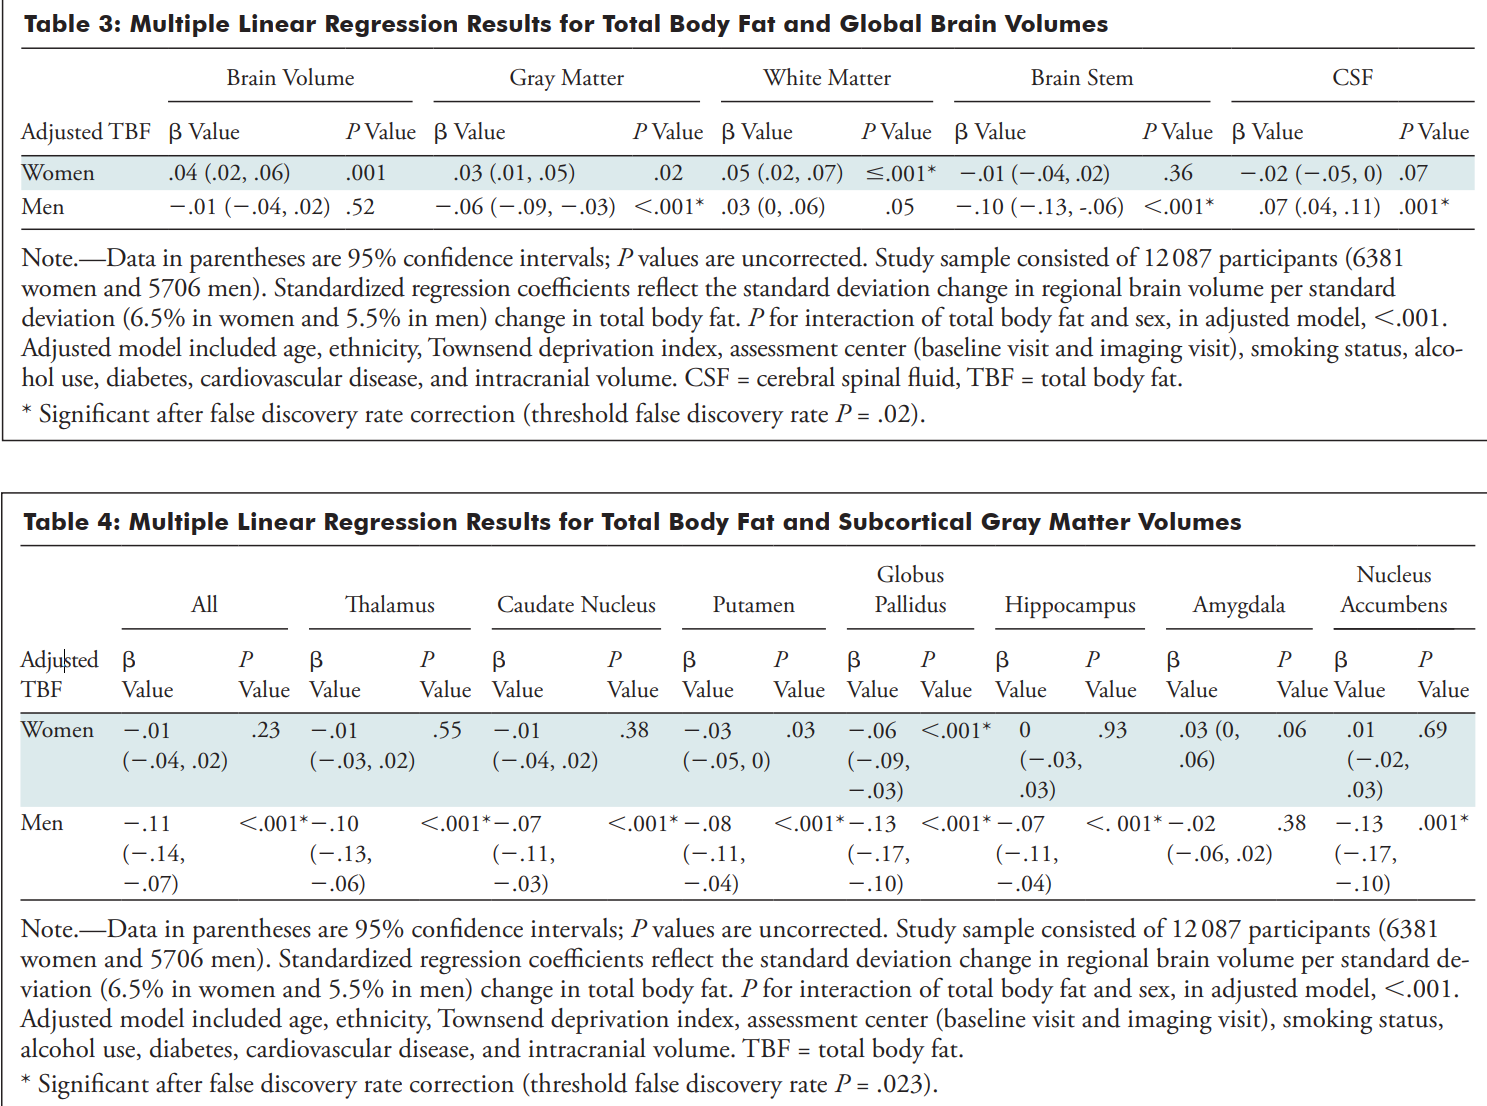
\includegraphics[width=\linewidth]{assets/brain_tables.png}\end{center}


\worklines{3}

\end{minipage}\par\vspace{5pt}

\par\addvspace{8pt}\noindent\begin{minipage}{\linewidth}

\section{往年题}

\subsection{单项选择题}

\Question{R24-M1}{自变量缩放与回归系数}

在含截距的多重线性回归中，将每个自变量 \(X_j\) 改写为 \(X_j^*=cX_j\)，其中 \(c>0\)。重新拟合后，偏回归系数与标准化偏回归系数如何变化？


\begin{choices}

\item 偏回归系数乘以 \(c\)，标准化偏回归系数不变。

\item 偏回归系数除以 \(c\)，标准化偏回归系数不变。

\item 二者均除以 \(c\)。

\item 二者均保持不变。

\item 偏回归系数不变，标准化偏回归系数乘以 \(c\)。

\end{choices}

\end{minipage}\par\vspace{5pt}

\par\addvspace{8pt}\noindent\begin{minipage}{\linewidth}

\Question{R24-M2}{复相关系数等于1}

在含截距且总平方和非零的多重线性回归中，复相关系数为1，以下哪项成立？


\begin{choices}

\item \(SS_{\text{残差}}=SS_{\text{总}}\)。

\item \(SS_{\text{回归}}=SS_{\text{总}}\)。

\item \(MS_{\text{残差}}=MS_{\text{总}}\)。

\item \(SS_{\text{回归}}=0\)。

\item \(SS_{\text{残差}}<0\)。

\end{choices}

\end{minipage}\par\vspace{5pt}

\par\addvspace{8pt}\noindent\begin{minipage}{\linewidth}

\Question{R24-M11}{连接函数的作用对象}

广义线性模型中，连接函数 \(g\) 通常将哪一项与线性预测子 \(X_i^T\beta\) 联系起来？


\begin{choices}

\item 每一个观测值 \(Y_i\) 本身。

\item 条件均值 \(\mu_i=E(Y_i\mid X_i)\)。

\item 每一个残差的平方。

\item 所有自变量的算术均数。

\item 回归系数的样本方差。

\end{choices}

\end{minipage}\par\vspace{5pt}

\par\addvspace{8pt}\noindent\begin{minipage}{\linewidth}

\subsection{名词解释}

\Question{R24-D1}{连接函数}

解释：连接函数。


\worklines{1}

\end{minipage}\par\vspace{5pt}

\par\addvspace{8pt}\noindent\begin{minipage}{\linewidth}

\Question{R24-D2}{拟合优度检验}

解释：拟合优度检验。


\worklines{1}

\end{minipage}\par\vspace{5pt}

\par\addvspace{8pt}\noindent\begin{minipage}{\linewidth}

\Question{Z-D1}{广义线性模型（Generalized Linear Models, GLM）}

名词解释：广义线性模型（Generalized Linear Models, GLM）。


\worklines{1}

\end{minipage}\par\vspace{5pt}

\par\addvspace{8pt}\noindent\begin{minipage}{\linewidth}

\Question{Z-D2}{连接函数（Link function）}

名词解释：连接函数（Link function）。


\worklines{1}

\end{minipage}\par\vspace{5pt}

\par\addvspace{8pt}\noindent\begin{minipage}{\linewidth}

\Question{Z-D10}{拟合优度检验（Goodness of Fit Test）}

名词解释：拟合优度检验（Goodness of Fit Test）。


\worklines{1}

\end{minipage}\par\vspace{5pt}

\par\addvspace{8pt}\noindent\begin{minipage}{\linewidth}

\subsection{简答题}

\Question{E21-1}{共线性的影响与识别}

什么是共线性？在进行广义线性模型分析时如果存在较严重的共线性，对分析结果会有什么影响？在进行 Cox 回归分析时，如何识别是否存在严重的共线性？


\worklines{3}

\end{minipage}\par\vspace{5pt}

\par\addvspace{8pt}\noindent\begin{minipage}{\linewidth}

\Question{R24-S4}{三种参数估计方法}

列举广义线性模型常用的3种参数估计方法，并简述其基本思想。


\worklines{3}

\end{minipage}\par\vspace{5pt}

\par\addvspace{8pt}\noindent\begin{minipage}{\linewidth}

\Question{Z-S1}{GLM的三个组成部分}

简述广义线性模型（GLM）的三个组成部分及其作用。


\worklines{3}

\end{minipage}\par\vspace{5pt}

\par\addvspace{8pt}\noindent\begin{minipage}{\linewidth}

\subsection{文献分析题}

\Question{E20-4}{自选文献评述}

每次都留了作业文献评述的作业，请你自选一篇提交。


\worklines{3}

\end{minipage}\par\vspace{5pt}


\clearpage\section{补充练习}

\begin{keyidea}[说明]以下为配合正文新编的补充练习，按题型编排。教学设定的数据不代表真实研究结果；解析见章末。\end{keyidea}

\par\addvspace{8pt}\noindent\begin{minipage}{\linewidth}

\subsection{单项选择题}

\Question{P1-M1}{加权最小二乘的权重}

某线性回归的均值结构设定正确，各观察相互独立，但误差方差不齐。已知甲、乙两条观察的条件误差方差分别为4和9。按正文的加权最小二乘原则，甲与乙的权重之比应为：

\begin{choices}

\item \(4/9\)。

\item \(2/3\)。

\item \(3/2\)。

\item \(9/4\)。

\item \(1\)。

\end{choices}

\end{minipage}\par\vspace{5pt}

\par\addvspace{8pt}\noindent\begin{minipage}{\linewidth}

\subsection{名词解释}

\Question{P1-D1}{似然函数}

名词解释：似然函数（Likelihood function）。

\worklines{1}

\end{minipage}\par\vspace{5pt}

\par\addvspace{8pt}\noindent\begin{minipage}{\linewidth}

\subsection{简答题}

\Question{P1-S1}{正态线性模型中的两种估计}

设各观察相互独立，\(Y_i\mid X_i\sim N(X_i^T\beta,\sigma^2)\)，其中\(\sigma^2\)为共同方差，设计矩阵满列秩。简述为什么极大似然估计与最小二乘估计给出相同的回归系数。若改为已知且不相等的方差\(\sigma_i^2\)，相应目标函数如何变化？

\worklines{3}

\end{minipage}\par\vspace{5pt}

\par\addvspace{8pt}\noindent\begin{minipage}{\linewidth}

\subsection{计算与综合分析题}

\Question{P1-C1}{从四格表写出似然与模型}

一项教学队列的固定随访期内，某二分类结局的频数如下。假定个体相互独立，同一暴露组内事件概率相同。
\begin{center}\begin{tabular}{lrr}\toprule
 & 发生事件 & 未发生事件\\\midrule
暴露组（\(X=1\)） & 30 & 70\\
非暴露组（\(X=0\)） & 10 & 90\\\bottomrule
\end{tabular}\end{center}
设\(\operatorname{logit}(p_x)=\alpha+\beta x\)。
\begin{enumerate}
\item 写出似然函数及对数似然函数，可略去与参数无关的常数。
\item 求\(\hat p_0,\hat p_1,\hat\alpha,\hat\beta\)，并写出拟合方程。
\item 分别求OR与两组事件概率之比，说明二者是否相同。
\end{enumerate}

\worklines{3}

\end{minipage}\par\vspace{5pt}


\clearpage\section{习题解析}

\begin{keyidea}[核对方式]按题号核对。缺失选项的补写及新编练习均在对应解析末尾说明。\end{keyidea}

\subsection{作业题}

\Answer{F1-1}{标准化、共线性与正态性诊断}

（1）标准化消除计量单位影响；\(\beta_j^*=\beta_j s_{X_j}/s_Y\)，表示控制其他变量时 \(X_j\) 增加1个标准差，\(Y\) 均值改变多少个标准差。比较幅度看绝对值。（2）\(R=\sqrt{R^2}\)，衡量 \(Y\) 与一组解释变量的线性关联。（3）检查残差模式、极端点及模型前提；交叉验证评估样本外预测误差。（4）检查共线性造成的系数不稳定与敏感性，但删变量应结合研究目标和混杂控制。（5）若 \(H_0\) 为服从所检验的正态分布，\(P<0.001\) 反而提供反对 \(H_0\) 的证据。回归中正态假定通常针对条件误差；估计了分布参数时不能直接套用普通 K--S 的临界分布。


\Answer{H1-1}{脂联素水平的影响因素}

\textbf{（1）建模与解释，1.5分。} 令 \(X_1\) 为 BMI，\(X_2\) 为 DY，\(X_3\) 为 LEP，\(X_4\) 为 FPG，以 ADI 为因变量： \[\widehat{\mathrm{ADI}}=58.199-1.030X_1-0.131X_2-0.811X_3-0.579X_4.\] 偏回归系数表示其他自变量固定时，该自变量增加一个单位所对应的 ADI 条件均值改变量。

\textbf{（2）系数检验，1.5分；（3）影响幅度，1分。} 原评分表如下：

\begin{longtable}[]{@{}lrrrrr@{}}
\toprule\noalign{}
变量 & 系数 & 标准误 & \(t\) & \(P\) & 标准化系数 \\
\midrule\noalign{}
\endhead
\bottomrule\noalign{}
\endlastfoot
BMI & −1.02978 & 0.530217 & −1.94 & 0.063 & −0.34312 \\
DY & −0.13113 & 0.211292 & −0.62 & 0.540 & −0.06653 \\
LEP & −0.81130 & 0.252699 & −3.21 & 0.004 & −0.56620 \\
FPG & −0.57873 & 0.447498 & −1.29 & 0.208 & −0.13939 \\
\end{longtable}

在 \(\alpha=0.05\) 下，仅 LEP 系数有统计学意义。标准化系数\textbf{绝对值}以 LEP 最大；不能直接比较带不同量纲的原始系数。

\textbf{（4）拟合，1.5分。} \(R^2=0.7312\)，\(R=0.8551\)，\(R^2_{\rm adj}=0.6882\)； \[R^2_{\rm adj}=1-(1-R^2)\frac{n-1}{n-p-1}.\] 还应检查线性、独立性、残差正态性和方差齐性，必要时以交叉验证评估预测误差。

\textbf{（5）随机部分与连接，1分。} 本例可先采用正态条件分布和恒等连接 \(g(\mu)=\mu\)；须用诊断评价是否合适。常见组合：正态---恒等、二项---logit、泊松---log、Gamma---倒数、逆高斯---\(1/\mu^2\)（典型连接的常数/符号可吸收到参数中）。变量连续并不自动意味着正态。

\textbf{（6）估计，1.5分。} 最小二乘使残差平方和最小；加权最小二乘使 \(\sum w_i(y_i-\mu_i)^2\) 最小，常取 \(w_i\propto1/\sigma_i^2\)；极大似然使观测数据的似然最大。原评分稿根据残差图建议加权最小二乘或极大似然。

\textbf{校正。} 图形只能提示异方差；极大似然本身不会自动消除异方差，需正确指定方差结构。Gauss--Markov 最优线性无偏性并不要求误差正态。


\Answer{H1-2}{肥胖与脑结构：文献分析}

\textbf{（1）} 横断面研究；数据来自 UK Biobank，并不因此成为此分析的前瞻性研究。暴露为肥胖指标 BMI/TBF，结局为 MRI 脑容量和结构指标。描述连续变量的均值、标准差或四分位数，分类变量用百分比；采用多重线性回归，报告标准化系数，调整年龄、种族、社会剥夺、中心、吸烟、饮酒、糖尿病和心血管病等因素，并检验 TBF 与性别的交互作用。

\textbf{（2）} Table 3 中女性总脑容量、灰质和白质体积与 TBF 呈正向关联；男性灰质和脑干体积呈负向关联，脑脊液体积呈正向关联。必须结合表中 \(P\) 值和多重比较阈值，而不是只看系数正负。Table 4 中男性除杏仁核外多项皮质下灰质体积均呈负向关联；女性以苍白球负向关联最明确。苍白球关联的性别差异 \(P<0.001\)（原评分稿）。

\textbf{答题边界。} 这是调整后的统计关联，不宜写成``脂肪增加导致脑体积改变''。对每项结果均说明性别、参照/单位、方向及统计学证据。


\subsection{往年题}

\Answer{R24-M1}{自变量缩放与回归系数}

\textbf{答案：B。}

对 \(X_j'=cX_j\) 且 \(c\ne0\)，\(b_j'=b_j/c\)。若 \(c>0\)，标准化偏回归系数不变；若 \(c<0\)，其符号反转而绝对值不变。\(c=0\) 时丢失变量信息，不适用上述等价变换。通常选择题默认 \(c>0\)。

\textbf{补写说明。} 原稿未记选项；选项为补写，并明确了常数为正的条件。


\Answer{R24-M2}{复相关系数等于1}

\textbf{答案：B。}

在含截距且总平方和非零的通常回归情形下，\(R^2=1\)，所以残差平方和为0，回归平方和等于总平方和。

\textbf{补写说明。} 原稿A---C保留；D、E为补写，并明确总平方和非零。


\Answer{R24-M11}{连接函数的作用对象}

\textbf{答案：B。}

GLM满足 \(g(\mu_i)=X_i^T\beta\)，连接作用于条件均值，而不是直接作用于观测值。

\textbf{补写说明。} 原稿第11题整题缺失；本题为围绕课程知识点新编的练习，并非恢复的往年原题。


\Answer{R24-D1}{连接函数}

将因变量的条件均值 \(\mu_i=E(Y_i\mid X_i)\) 与线性预测子 \(\eta_i=X_i^T\beta\) 联系起来的函数：\(g(\mu_i)=\eta_i\)。连接作用于均值，不是对观测值直接作同样变换。


\Answer{R24-D2}{拟合优度检验}

评价所指定模型与观测数据之间的不一致是否超出随机变异可以解释的范围。例如分组 Logistic 的 Pearson/偏差检验、Hosmer--Lemeshow 检验。\(P\) 值大只能表示未发现明显失拟；总体回归系数检验是比较含协变量模型与零模型，不能直接等同于绝对拟合优度检验。


\Answer{Z-D1}{广义线性模型（Generalized Linear Models, GLM）}

用随机部分、系统部分与连接函数推广普通线性回归的模型框架。随机部分通常为指数分布族；\(\eta=X^T\beta\)；\(g\{E(Y\mid X)\}=\eta\)。


\Answer{Z-D2}{连接函数（Link function）}

连接条件均值 \(\mu\) 与线性预测子 \(\eta\) 的函数 \(g\)，满足 \(g(\mu)=\eta\)，例如logit、log与恒等连接。


\Answer{Z-D10}{拟合优度检验（Goodness of Fit Test）}

检验模型预测与观测的不一致是否超过随机变异可以解释的范围。模型与饱和模型的偏差、分组Pearson或HL检验可用于特定情形。拟合优度与协变量的总体显著性、预测区分度应区分。


\Answer{E21-1}{共线性的影响与识别}

共线性指解释变量之间存在精确或近似线性关系。完全共线性使参数不能唯一估计；严重近似共线性会放大标准误、扩大置信区间，使系数大小和符号对数据或变量组合敏感，个别检验效能下降。

Cox 模型中检查设计矩阵的相关结构、秩、条件数和 VIF/GVIF。对一个数值变量，\(\mathrm{VIF}_j=1/(1-R_j^2)\)，其中 \(R_j^2\) 来自该变量对其余解释变量的辅助回归。多自由度因子应结合 \(\mathrm{GVIF}^{1/(2df)}\)，不能将未调整 GVIF 与单一 VIF 混用。5或10是经验警戒值，不是严格判据。PH 检验与共线性诊断解决不同问题。


\Answer{R24-S4}{三种参数估计方法}

按课程口径：最小二乘、加权最小二乘、极大似然。分别最小化残差平方和、带权残差平方和，以及最大化似然。普通 GLM 通常以极大似然估计，并通过迭代加权最小二乘求解；Cox 模型通常使用偏似然。详见 题1.2（6）。


\Answer{Z-S1}{GLM的三个组成部分}

随机部分指定 \(Y\mid X\) 的概率分布及方差结构；系统部分为 \(\eta_i=\beta_0+\sum_j\beta_jx_{ij}\)；连接函数令 \(g(\mu_i)=\eta_i\)，使不同类型结局的条件均值能用线性预测子描述。


\Answer{E20-4}{自选文献评述}

开放题，无唯一标准答案。可选本章 题1.3 的文献，依次写研究问题、人群与设计、暴露/结局/协变量、模型选择依据、关键估计值及置信区间、偏倚与局限。也可选 题2.2 或 题3.2，但须围绕所选文章展开，而非拼接模型定义。原材料 对本题只有题干，未附评述正文。


\subsection{补充练习}

\Answer{P1-M1}{加权最小二乘的权重}

\textbf{答案：D。} 权重与条件误差方差的倒数成正比，故
\[\frac{w_{\text{甲}}}{w_{\text{乙}}}=\frac{1/4}{1/9}=\frac94.\]
这里取的是\textbf{方差}的倒数，不是标准差的倒数；方差较大的观察获得较小权重。



\Answer{P1-D1}{似然函数}

给定已经观察到的样本，将其联合概率质量函数或联合概率密度函数看成未知参数的函数，称为似然函数。独立观察时，
\[L(\theta;y_1,\ldots,y_n)=\prod_{i=1}^{n}f(y_i;\theta).\]
样本值固定，参数变化；使该函数最大的参数值为极大似然估计。似然函数不应解释为“给定样本后参数的概率分布”。



\Answer{P1-S1}{正态线性模型中的两种估计}

同方差正态模型的对数似然为
\[\ell(\beta,\sigma^2)=-\frac n2\log(2\pi\sigma^2)
-\frac{1}{2\sigma^2}\sum_{i=1}^{n}(y_i-X_i^T\beta)^2.\]
对任一固定的正方差，最大化对数似然等价于最小化残差平方和；共同方差未知时，联合极大化所得\(\hat\beta\)也相同。满列秩保证通常最小二乘解唯一。

若各\(\sigma_i^2\)已知且不等，关于\(\beta\)需最小化的部分变为
\[\sum_i\frac{(y_i-X_i^T\beta)^2}{\sigma_i^2},\]
即以\(1/\sigma_i^2\)为权重的加权最小二乘。这里比较的是\textbf{回归系数}的估计，不是在说方差的极大似然估计与无偏估计相同。



\Answer{P1-C1}{从四格表写出似然与模型}

\textbf{（1）} 令\(p_0=e^\alpha/(1+e^\alpha)\)、\(p_1=e^{\alpha+\beta}/(1+e^{\alpha+\beta})\)，则
\[L\propto p_1^{30}(1-p_1)^{70}p_0^{10}(1-p_0)^{90},\]
\[\ell=30(\alpha+\beta)+10\alpha
-100\log(1+e^{\alpha+\beta})-100\log(1+e^\alpha)+C.\]
\textbf{（2）} 两组各有一个可自由估计的概率，因此\(\hat p_0=0.10\)、\(\hat p_1=0.30\)。
\[\hat\alpha=\log\frac{10}{90}=-2.1972,\qquad
\hat\beta=\log\frac{30\times90}{70\times10}=1.3499.\]
拟合方程为\(\operatorname{logit}(\hat p_x)=-2.1972+1.3499x\)。

\textbf{（3）} \(\widehat{\mathrm{OR}}=27/7=3.8571\)，事件概率之比为\(0.30/0.10=3\)。两者不同，因为OR比较的是\(p/(1-p)\)。本题为固定随访期队列的完整频数，可直接算概率；不能把同样做法无条件套到按病例、对照抽样的研究。
\EndExercises

\chapter{Logistic回归模型（一）}
\sourcepages{3}{1-3}
\subsection*{主要内容}
\begin{enumerate}
\item Logistic回归的基本概念、非条件Logistic回归。
\item 配比设计资料的条件Logistic回归分析。
\item 多分类结局资料的Logistic回归分析。
\item 有序分类结局资料的Logistic回归分析。
\item Logistic回归模型的正确应用及软件实现。
\end{enumerate}
\section{Logistic回归的基本概念}
\sourcepages{3}{4}
Logistic回归是医学研究中最常用的多因素分析方法之一。理解该模型的关键在于对数优势尺度：模型在logit尺度上是线性、可加的，系数为对数OR；换算到概率尺度后，同一OR对应的概率差随基线水平而变化。将OR等同于RR、将OR为3表述为死亡率增加3倍等常见错误，均源于两种尺度的混淆。

本章另一重点是统计推断。参数由迭代求得，检验与区间估计依赖大样本近似，Wald检验、似然比检验与比分检验三者并存，了解其来源有助于在小样本或稀疏数据时作出选择。最后一节的条件logistic回归用于配对设计，其基本思想是通过条件化消去对子参数，这一思想在第5章的Cox回归中再次出现。
\subsection{Logistic回归模型}
\sourcepages{3}{5-12}
\textbf{例1（横断面研究）} 在研究医院抢救急性心肌梗塞（AMI）患者能否成功的危险因素的调查中，某医院收集了5年中该院所有的AMI患者的抢救病史（有关危险因素很多，由于篇幅有限，本例仅列出3个），共200例。
\begin{itemize}
\item $Y=0$ 表示抢救成功，$Y=1$ 表示死亡。
\item $X_1=1$ 表示抢救前已发生休克，$X_1=0$ 表示抢救前未发生过休克。
\item $X_2=1$ 表示抢救前发生心衰，$X_2=0$ 表示抢救前未发生心衰。
\item $X_3=1$ 表示患者从开始AMI症状到抢救时已超过12小时（即未能及时把患者送往医院），$X_3=0$ 表示未超过12小时。
\end{itemize}
\ctable{表1\quad AMI患者的抢救危险因素资料}{
\begin{tabular}{cccccccc}\toprule
\multicolumn{4}{c}{$Y=0$（在医院抢救成功）}&\multicolumn{4}{c}{$Y=1$（未能抢救成功而死亡）}\\\cmidrule(lr){1-4}\cmidrule(lr){5-8}
$X_1$&$X_2$&$X_3$&$N$&$X_1$&$X_2$&$X_3$&$N$\\\midrule
0&0&0&35&0&0&0&4\\0&0&1&34&0&0&1&10\\0&1&0&17&0&1&0&4\\0&1&1&19&0&1&1&15\\1&0&0&17&1&0&0&6\\1&0&1&6&1&0&1&9\\1&1&0&6&1&1&0&6\\1&1&1&6&1&1&1&6\\\bottomrule
\end{tabular}}

$Y$ 是二分类变量，服从二项分布，事件发生的概率记为 $P$。
\begin{align*}
\ln\left(\frac{P}{1-P}\right)&=\beta_0+\beta_1x_1+\beta_2x_2+\beta_3x_3,\\
\ln\left(\frac{P}{1-P}\right)&=\logit(P)=\beta_0+\beta_1x_1+\beta_2x_2+\beta_3x_3.
\end{align*}
\cfigure{图1\quad Logistic回归中线性预测量 $\eta$（logit值）与 $P$ 的关系示意图}{
\begin{tikzpicture}\begin{axis}[width=10cm,height=6cm,axis lines=middle,xmin=-5,xmax=5,ymin=0,ymax=1.02,xtick={-5,-4,...,5},ytick={.1,.2,...,1},xlabel={$\eta$},ylabel={$P$}]
\addplot[PlotPrimary,line width=1pt,domain=-5:5,samples=101]{1/(1+exp(-x))};
\end{axis}\end{tikzpicture}}
\textbf{Logistic回归模型}
\begin{align*}
\ln\left(\frac P{1-P}\right)&=\beta_0+\beta_1x_1+\beta_2x_2+\cdots+\beta_mx_m,\\
\logit(P)&=\beta_0+\beta_1x_1+\beta_2x_2+\cdots+\beta_mx_m,\\
P&=\frac{e^{\beta_0+\beta_1x_1+\cdots+\beta_mx_m}}{1+e^{\beta_0+\beta_1x_1+\cdots+\beta_mx_m}}
 =\frac{1}{1+e^{-(\beta_0+\beta_1x_1+\cdots+\beta_mx_m)}}.
\end{align*}

\begin{annotation}
$P/(1-P)$ 称为优势（odds）；$\eta=\beta_0+\beta_1x_1+\beta_2x_2+\beta_3x_3$ 为线性预测量。图1横轴是 $\eta=\logit(P)$，取值 $(-\infty,\infty)$；纵轴是概率 $P\in(0,1)$，二者由单调的Logistic曲线一一对应。

logit形式与概率形式是同一模型的两种写法：前者在logit尺度上是线性的，系数直接对应对数优势比，便于解释影响因素；后者把 $\eta$ 反变换回概率，便于给出个体的预测概率。选用哪种写法取决于报告目的，不改变模型本身。
\end{annotation}
\textbf{Logistic回归模型的连接函数}
\begin{itemize}
\item 分布族family：二项分布binomial。
\item 连接函数link：logit。
\end{itemize}
\[
\eta=g(\mu)=\logit(P),\qquad \logit(P)=\ln\left(\frac{P}{1-P}\right).
\]
\begin{annotation}这种变换称为logit变换。\end{annotation}
\subsection{参数的估计方法}
\sourcepages{3}{13-19}
\begin{itemize}
\item 因为资料不满足“方差齐性”的条件，故LSE不适宜。
\item 加权最小二乘估计（weighted least squared, WLS），其权重是方差的倒数，方差越大权重越小，方差越小权重越大。
\item 极大似然估计（maximum likelihood estimation, MLE），构建似然函数，根据样本数据，找到最有可能产生样本观察值的参数值。
\end{itemize}
\begin{annotation}$\beta$ 的估计值可写作 $\widehat\beta$ 或英文字母 $b$。\end{annotation}
\begin{align*}
L(\theta\mid y_1,y_2,\ldots,y_n)
&=f(y_1,y_2,\ldots,y_n\mid\theta)\\
&=f(y_1\mid\theta)f(y_2\mid\theta)\cdots f(y_n\mid\theta)
=\prod_{i=1}^nf(y_i\mid\theta).
\end{align*}
\[
\text{对数似然函数：}\quad \ln L(\theta\mid y_1,y_2,\ldots,y_n),
\]
\[
\max L(\theta\mid y_1,y_2,\ldots,y_n),\qquad
\frac{\partial\ln L(\theta\mid y_1,y_2,\ldots,y_n)}{\partial\theta}=0.
\]
\begin{annotation}
$\theta$ 是参数，$y_i$ 是第 $i$ 个观测值。似然函数与联合概率函数是同一表达式，区别在于把谁看作变量：固定参数看 $\bm y$ 是概率，固定 $\bm y$ 看参数是似然。独立观测的似然是连乘，取对数后变为连加；令一阶导数（得分）为0求驻点，再由二阶导数判断是否为最大值。
\end{annotation}
\begin{derivation}{一般Logistic回归的得分、信息阵与IRLS}
\dpart{假设}$Y_i\mid\bm x_i\sim\text{Bernoulli}(\pi_i)$，$i=1,\ldots,n$ 条件独立，$\logit(\pi_i)=\eta_i=\bm x_i^\top\bm\beta$，$\bm X$ 为 $n\times p$ 列满秩设计矩阵。
\dpart{关键等式}对数似然
\[
\ell(\bm\beta)=\sum_{i=1}^n\{y_i\log\pi_i+(1-y_i)\log(1-\pi_i)\}
=\sum_{i=1}^n\{y_i\eta_i-\log(1+e^{\eta_i})\}.
\]
由 $\partial\log(1+e^{\eta})/\partial\eta=\pi$、$\partial\pi/\partial\eta=\pi(1-\pi)$，得
\begin{gather*}
\bm U(\bm\beta)=\frac{\partial\ell}{\partial\bm\beta}=\sum_i(y_i-\pi_i)\bm x_i=\bm X^\top(\bm y-\bm\pi),\\
\frac{\partial^2\ell}{\partial\bm\beta\,\partial\bm\beta^\top}=-\sum_i\pi_i(1-\pi_i)\bm x_i\bm x_i^\top=-\bm X^\top\bm W\bm X,
\end{gather*}
其中 $\bm W=\diag\{\pi_i(1-\pi_i)\}$。Hessian不含 $y_i$，故观测信息等于期望（Fisher）信息 $\bm I(\bm\beta)=\bm X^\top\bm W\bm X$。
\dpart{结论}(1) 当 $0<\pi_i<1$、$\bm X$ 列满秩时 $\bm X^\top\bm W\bm X$ 正定，$\ell$ 是严格凹函数，若有限的最大值点存在则唯一。(2) MLE满足 $\bm X^\top(\bm y-\widehat{\bm\pi})=\bm 0$；含截距时 $\sum_iy_i=\sum_i\widehat\pi_i$。(3) 大样本下 $\widehat{\bm\beta}\approx N\{\bm\beta,\bm I(\bm\beta)^{-1}\}$，用 $\widehat{\Cov}(\widehat{\bm\beta})=(\bm X^\top\widehat{\bm W}\bm X)^{-1}$，其对角元开方即软件输出的标准误。
\dpart{迭代算法}Fisher scoring（对典型连接即Newton--Raphson）：
\[
\bm\beta^{(t+1)}=\bm\beta^{(t)}+(\bm X^\top\bm W^{(t)}\bm X)^{-1}\bm X^\top(\bm y-\bm\pi^{(t)}).
\]
定义工作响应 $z_i^{(t)}=\eta_i^{(t)}+\dfrac{y_i-\pi_i^{(t)}}{\pi_i^{(t)}(1-\pi_i^{(t)})}$，上式可改写为
\[
\bm\beta^{(t+1)}=(\bm X^\top\bm W^{(t)}\bm X)^{-1}\bm X^\top\bm W^{(t)}\bm z^{(t)},
\]
即以 $\bm W^{(t)}$ 为权重、$\bm z^{(t)}$ 为响应的一次加权最小二乘；权重随 $\bm\pi$ 更新、反复迭代，故称迭代加权最小二乘（IRLS）。分组资料（第 $i$ 组 $n_i$ 例、$y_i$ 例发生）只需把 $\pi_i$ 换成 $n_i\pi_i$、权重换成 $n_i\pi_i(1-\pi_i)$。
\dpart{解释}以例1的8个协变量组合为分组资料，从 $\bm\beta^{(0)}=\bm 0$ 起迭代，数步即收敛到表2的估计值（$-2.0858$, $1.1098$, $0.7028$, $0.9751$），标准误取自 $(\bm X^\top\widehat{\bm W}\bm X)^{-1}$。
\end{derivation}
将上述迭代公式写成R代码，对例1的分组资料自$\bm\beta^{(0)}=\bm0$开始迭代：
\par\noindent
\begin{coursecode}{R}
ami <- data.frame(x1=rep(c(0,1),each=4), x2=rep(rep(c(0,1),each=2),2), x3=rep(c(0,1),4),
                  alive=c(35,34,17,19,17,6,6,6), dead=c(4,10,4,15,6,9,6,6))
X <- cbind(1, as.matrix(ami[,1:3])); y <- ami$dead; n <- ami$dead+ami$alive
beta <- rep(0,4)
for(t in 1:5){
  p <- plogis(drop(X%*%beta)); W <- n*p*(1-p)           # 当前的概率和权重
  beta <- beta + solve(t(X)%*%(W*X), t(X)%*%(y-n*p))    # Fisher scoring一步
  cat("第",t,"次:",sprintf("%9.5f",beta),"\n")
}
sqrt(diag(solve(t(X)%*%(W*X))))                          # 标准误
\end{coursecode}
\begin{routput}
第 1 次:  -1.67585   0.88648   0.55088   0.73037 
第 2 次:  -2.04856   1.08991   0.68962   0.95113 
第 3 次:  -2.08550   1.10964   0.70273   0.97486 
第 4 次:  -2.08584   1.10982   0.70285   0.97509 
第 5 次:  -2.08584   1.10982   0.70285   0.97509 
                 x1        x2        x3 
0.3512559 0.3484879 0.3291858 0.3439633 
\end{routput}
第4次迭代后，估计值小数点后5位不再变化，结果与\texttt{glm()}相同（\texttt{glm()}报告迭代3次，是因为其收敛判据为偏差的相对变化）。标准误为信息阵逆矩阵对角元的平方根。该算法的每一步依次为：由当前估计计算概率与权重，求解一次加权最小二乘，重复直至收敛。

\textbf{有限MLE的存在性}\quad 上面的严格凹性只保证“若有最大值点则唯一”，并不保证最大值点有限。
\begin{itemize}
\item \textbf{完全分离}：存在 $\bm b$ 使 $y_i=1$ 时 $\bm x_i^\top\bm b>0$、$y_i=0$ 时 $\bm x_i^\top\bm b<0$。沿 $\bm b$ 方向放大系数，似然单调增至1，MLE不存在（某些系数趋于 $\pm\infty$）。
\item \textbf{准完全分离}：上述不等式中允许等号，且至少一侧有等号成立。似然仍有上确界而达不到，相应系数发散。
\item \textbf{四格表的情形}：$\widehat\beta=\ln\{ad/(bc)\}$ 要求四个格子都为正。任一格为0（如暴露组无病例），$\widehat\beta=\pm\infty$，正是准完全分离。
\item \textbf{识别与处理}：软件常给出“拟合概率为0或1”的警告，系数和标准误异常大、迭代不收敛。可合并稀疏类别、检查编码，或改用Firth惩罚似然、精确Logistic回归。不能简单删去引起分离的变量后照常解释。
\end{itemize}
\subsubsection{四格表资料的极大似然估计}
\ctable{表10\quad 暴露者与非暴露者发病与不发病的概率}{\renewcommand{\arraystretch}{1.8}\begin{tabular}{lcc}\toprule
&暴露，$x=1$&非暴露，$x=0$\\\midrule
发病，$y=1$&$P_1=\dfrac{e^{\alpha+\beta}}{1+e^{\alpha+\beta}}$&$P_0=\dfrac{e^\alpha}{1+e^\alpha}$\\
不发病，$y=0$&$1-P_1=\dfrac1{1+e^{\alpha+\beta}}$&$1-P_0=\dfrac1{1+e^\alpha}$\\\bottomrule\end{tabular}}
\begin{align*}
L&=\left(\frac{e^{\alpha+\beta}}{1+e^{\alpha+\beta}}\right)^a
\left(\frac{e^\alpha}{1+e^\alpha}\right)^b
\left(\frac1{1+e^{\alpha+\beta}}\right)^c
\left(\frac1{1+e^\alpha}\right)^d,\\
\ln L&=a(\alpha+\beta)-a\ln(1+e^{\alpha+\beta})+b\alpha-b\ln(1+e^\alpha)\\
&\qquad-c\ln(1+e^{\alpha+\beta})-d\ln(1+e^\alpha)\\
&=a(\alpha+\beta)+b\alpha-(a+c)\ln(1+e^{\alpha+\beta})-(b+d)\ln(1+e^\alpha),\\
\frac{\partial\ln L}{\partial\alpha}&=a+b-\frac{(a+c)e^{\alpha+\beta}}{1+e^{\alpha+\beta}}-\frac{(b+d)e^\alpha}{1+e^\alpha},\\
\frac{\partial\ln L}{\partial\beta}&=a-\frac{(a+c)e^{\alpha+\beta}}{1+e^{\alpha+\beta}}.
\end{align*}
令 $\partial\ln L/\partial\alpha=0$，$\partial\ln L/\partial\beta=0$，得：
\[
\widehat\alpha=\ln\frac bd,\qquad \widehat\beta=\ln\frac{ad}{bc},\qquad
\logit(P)=\alpha+\beta x=\ln\frac bd+\ln\frac{ad}{bc}\,x.
\]

\begin{annotation}由样本资料和极大似然估计得到回归方程。四格表是饱和模型，MLE等于观察比例对应的logit：$\widehat\alpha$ 为非暴露组的对数优势，$\widehat\beta$ 为对数OR。\end{annotation}
\sourcepages{3}{20}
\ctable{表2\quad 例1的参数估计与Wald检验结果}{\begin{tabular}{lrrrrr}\toprule
变量名&$\widehat\beta$&$\SE(\widehat\beta)$&Wald $\chi^2$&$P$值&OR\\\midrule
常数项&$-2.0858$&0.3513&35.2632&0.0001&---\\
$X_1$&1.1098&0.3485&10.1422&0.0014&3.034\\
$X_2$&0.7028&0.3292&4.5587&0.0328&2.019\\
$X_3$&0.9751&0.3440&8.0365&0.0046&2.651\\\bottomrule\end{tabular}}
\[
\logit(P)=-2.0858+1.1098X_1+0.7028X_2+0.9751X_3.
\]
\subsection{回归系数的意义}
\sourcepages{3}{21-29}
如何正确理解回归系数 $\beta(b)$ 的意义？
\begin{annotation}
$\beta$ 是总体参数，$b$（或 $\widehat\beta$）是它的估计值。线性回归中，$\beta_j$ 是其他变量固定时 $x_j$ 每增加1个单位 $\E(Y)$ 的改变量，在概率尺度上是常数；Logistic回归中 $\beta_j$ 是logit（对数优势）尺度上的改变量，换算到概率尺度后不再是常数（见下文）。
\end{annotation}
\begin{align*}
\text{发生休克：}\quad \ln\frac{P^*}{1-P^*}&=-2.0858+1.1098\times1+0.7028X_2+0.9751X_3,\\
\text{无休克：}\quad \ln\frac{P}{1-P}&=-2.0858+1.1098\times0+0.7028X_2+0.9751X_3,\\
\text{两式相减：}\quad \ln\left(\frac{P^*}{1-P^*}\Big/\frac{P}{1-P}\right)&=\ln(\OR)=1.1098,\\
\OR&=e^{1.1098}=3.034.
\end{align*}
\begin{annotation}
优势（odds）是同一组内事件发生概率与不发生概率之比 $P/(1-P)$；优势比（OR）是两组优势之比。在心衰、抢救是否及时相同的条件下，发生休克者死亡的优势是未休克者的3.034倍。
\end{annotation}
\textbf{常数项的含义}
\begin{itemize}
\item 常数项 $\widehat\beta_0=-2.0858$，表示在其它自变量均为零时死亡与不死亡优势的自然对数值。
\item $\exp(\widehat\beta_0)=0.1242$ 是无休克、无心衰和抢救及时组死亡与不死亡的比值。当死亡概率很低时，不死亡的概率接近1，该值近似等于死亡率。
\end{itemize}
\begin{annotation}当 $P$ 很小时，$P/(1-P)\approx P$。本例该组的模型死亡概率为 $\exp(\widehat\beta_0)/\{1+\exp(\widehat\beta_0)\}=0.1105$，与0.1242已有差别，故“优势近似概率”只适用于罕见结局。截距的这种解释还要求研究设计能估计绝对风险（横断面或队列资料）；病例对照资料的截距受抽样比例影响，不能这样解释。\end{annotation}
$\beta_i$ 表示当其它因素被控制后，$X$ 每改变一个单位，优势比（比值比，OR）的对数值（LnOR）。
\[
\beta=\ln\left[\frac{P(D=1\mid X^*)/P(D=0\mid X^*)}{P(D=1\mid X)/P(D=0\mid X)}\right]=\ln\OR,
\qquad e^\beta=\OR.
\]
当结局变量赋值为1表示死亡等危险事件时：
\begin{itemize}
\item 如果回归系数为正值，$\exp(\widehat\beta)>1$，该因素是危险因素。
\item 如果回归系数为负值，$\exp(\widehat\beta)<1$，该因素是保护因素。
\item 本例中3个因素的回归系数均为正值，说明休克、心衰和未能及时抢救都是增加死亡优势的危险因素。
\end{itemize}
\begin{sikao}[OR与RR的区别]
“休克者死亡的优势是未休克者的3.03倍”不能表述为“休克者的死亡风险是未休克者的3倍”。以第1章合并后的四格表为例（未调整其他因素）：
\begin{center}\small
\begin{tabular}{lcc}\toprule
&死亡率&优势$P/(1-P)$\\\midrule
休克（62例）&$27/62=0.435$&$0.771$\\
无休克（138例）&$33/138=0.239$&$0.314$\\\midrule
比值&RR$=1.82$&OR$=2.45$\\\bottomrule
\end{tabular}
\end{center}
死亡率之比为1.82，而OR为2.45。由$\OR=\RR\times\dfrac{1-P_0}{1-P_1}$可知，结局越常见，二者差别越大；仅当两组发生率均很低（一般低于10\%）时，$\OR\approx\RR$。本例死亡率在20\%--45\%之间，OR明显夸大了相对风险。

OR的广泛使用有两方面原因：logit连接保证概率位于$(0,1)$内，具有良好的数学性质；病例对照研究只能估计OR，且OR在病例对照抽样下保持不变，条件logistic回归即以此为基础。报告时应表述为“优势是……倍”；结局常见且需要RR时，可采用log连接的二项回归或稳健Poisson回归另行估计。
\end{sikao}
自变量可以是连续型的定量变量、两分类或多分类的定性变量。
\begin{enumerate}
\item 对于连续型的定量变量，$\beta_i$ 表示当其它因素被控制后，$X$ 每改变一个单位，优势比的对数值（LnOR）。
\item 对于两分类的定性变量，类别间互相的比较。
\item 对于多分类的定性变量，采用哑变量变换，与参照组的比较。
\end{enumerate}
\begin{annotation}例如母乳喂养知识得分的OR为1.10：其他因素不变时，得分每增加1分，长时间母乳喂养的\emph{优势}乘以1.10（增加10\%），并不是概率增加10\%或10个百分点。\end{annotation}
\begin{derivation}{OR与概率尺度上的效应}
\dpart{假设}$\logit\pi(\bm x)=\beta_0+\beta_jx_j+\sum_{k\ne j}\beta_kx_k$，$x_j$ 以线性项进入模型，且不与其他变量构成交互项。
\dpart{关键等式}其他变量固定，$x_j$ 由 $x$ 变为 $x+\Delta x$，两优势之比
\[
\OR(\Delta x)=\frac{\pi(x+\Delta x)/\{1-\pi(x+\Delta x)\}}{\pi(x)/\{1-\pi(x)\}}=\exp(\beta_j\Delta x),
\]
与 $x$ 和其他变量的取值无关。而在概率尺度上，
\[
\frac{\partial\pi}{\partial x_j}=\beta_j\,\pi(1-\pi).
\]
\dpart{结论}OR对所有个体相同（这是模型假设），但概率的改变量随基线概率而变：$\pi=0.5$ 时最大（$\beta_j/4$），$\pi$ 接近0或1时很小。以休克为例（OR=3.034），无心衰、抢救及时者死亡概率由0.110升至0.274，增加16.4个百分点；已有心衰且抢救不及时者由0.399升至0.669，增加26.9个百分点。
\dpart{解释}若 $x_j$ 有交互项或非线性项（如 $x_j^2$、样条），$\exp(\beta_j)$ 本身不再是“$x_j$ 每增加1单位的OR”，需按完整的线性预测量计算指定比较的OR。
\end{derivation}
\textbf{条件OR与边际OR}\quad 模型中的OR是\emph{调整其他协变量后}的条件OR。即使没有混杂，条件OR与边际（总体平均）OR也可以不同，这称为OR的不可折叠性（第6章）。例：$Z$ 取0、1各半且与 $X$ 独立，$\logit\pi=-1.5+\ln4\cdot x+3z$。$Z=0$ 层 $\pi(1)=0.472$、$\pi(0)=0.182$，$Z=1$ 层 $\pi(1)=0.947$、$\pi(0)=0.818$，两层OR都是4；合并后 $\pi(1)=0.709$、$\pi(0)=0.500$，边际OR为2.44。因此不同模型（调整变量不同）的OR不能简单比较大小，比较前要说明各自的调整集合。例1中休克的粗OR为2.455，调整心衰、抢救是否及时后为3.034，这一差别同时包含混杂与不可折叠性。

\textbf{病例对照抽样}\quad 若病例与对照的抽样比例分别为 $s_1$、$s_0$，且抽样只依赖结局 $Y$、不依赖 $\bm x$，则样本中
\[
\logit P(Y=1\mid\bm x,\text{被抽中})=\underbrace{\beta_0+\ln(s_1/s_0)}_{\text{截距改变}}+\bm x^\top\bm\beta .
\]
斜率 $\bm\beta$（从而OR）不变，可以照常估计；截距被抽样比例平移，故病例对照资料不能由模型直接得到绝对风险或预测概率，除非另有外部信息（如人群发病率）校正截距。若抽样还依赖 $\bm x$（如按暴露选对照），斜率也会有偏。
\subsection{回归系数的假设检验}
\sourcepages{3}{30-31}
检验模型中一个或者几个总体回归系数是否等于0。
\[
H_0:\beta_i=0\quad(\text{或联合地 }H_0:\beta_{j_1}=\cdots=\beta_{j_q}=0).
\]
假设是对未知的总体参数作出的约束；$\widehat\beta_i$ 是由样本算出的估计值，检验的正是它与0的差别能否用抽样误差解释，故 $H_0$ 中不应写 $\widehat\beta_i$。
有三种检验方法：Wald检验、似然比检验、比分检验。
\subsubsection{Wald检验}
\sourcepages{3}{32-33}
\[
z=\frac{\widehat\beta-0}{\SE(\widehat\beta)},\qquad
\text{Wald }\chi^2=z^2=\frac{(\widehat\beta-0)^2}{\Var(\widehat\beta)}.
\]
回归系数估计值的95\%CI：
\[
\widehat\beta-1.96\SE(\widehat\beta)\ \sim\ \widehat\beta+1.96\SE(\widehat\beta).
\]
OR值的95\%CI：
\[
e^{\widehat\beta-1.96\SE(\widehat\beta)}\ \sim\ e^{\widehat\beta+1.96\SE(\widehat\beta)}.
\]
\begin{annotation}依据是MLE的大样本正态性：$H_0:\beta=0$ 成立时 $z$ 近似服从标准正态分布，$z^2$ 近似服从 $\chi^2_1$，临界值 $1.96^2=3.84$。这是渐近结论，小样本或系数很大（接近分离）时Wald检验可能不可靠。OR的置信区间由系数区间取指数得到，因此关于OR不对称。报告时应同时给出OR、95\%置信区间和 $P$ 值。\end{annotation}
\ctable{休克变量的Wald检验与区间估计}{\begin{tabular}{lrrrrr}\toprule
变量&回归系数&标准误&系数下限&系数上限&Wald统计量\\\midrule
休克&1.110&0.349&0.427&1.793&10.142\\\bottomrule
\end{tabular}\par\smallskip\begin{tabular}{lrrrrr}\toprule
变量&自由度&$P$值&OR&OR下限&OR上限\\\midrule
休克&1&0.001&3.034&1.532&6.007\\\bottomrule\end{tabular}}
\subsubsection{似然比检验}
\sourcepages{3}{34-36}
通过比较两个相嵌套模型的对数似然函数值进行，统计量 $G$ 等于两模型偏差（deviance）之差。
\begin{align*}
G&=D_P-D_K\\
&=-2\bigl(\text{模型 $P$ 的对数似然函数}-\text{模型 $K$ 的对数似然函数}\bigr).
\end{align*}
其中，模型 $P$ 中的变量是模型 $K$ 中的一部分，模型 $K$ 中剩余的就是我们要检验的变量。$H_0$ 成立时 $G$ 近似服从自由度为 $K-P$ 的 $\chi^2$ 分布。
\begin{annotation}模型 $P$ 含 $P$ 个参数，模型 $K$ 含 $K$ 个参数，$K>P$。自由度 $K-P$ 等于 $H_0$ 施加的独立约束个数，即被检验的参数个数（一个多分类变量的 $c-1$ 个哑变量要合起来检验时，自由度为 $c-1$）。\end{annotation}
\ctable{表3\quad 拟合的Logistic回归模型的对数似然函数值}{\begin{tabular}{clrr}\toprule
编号&模型中的变量&对数似然函数值&参数个数\\\midrule
1&常数项&$-122.172$&1\\
2&常数项+休克&$-118.367$&2\\
3&常数项+心衰&$-119.549$&2\\
4&常数项+及时&$-118.667$&2\\
5&常数项+休克+心衰&$-115.557$&3\\
6&常数项+休克+及时&$-113.599$&3\\
7&常数项+心衰+及时&$-116.491$&3\\
8&常数项+休克+心衰+及时&$-111.308$&4\\\bottomrule\end{tabular}}
\begin{annotation}
模型5嵌套于模型8，两者只差变量“及时”。$H_0$：调整休克与心衰后，“及时”的系数为0。若加入该变量后对数似然增加较多，$G$ 就大；$G>\chi^2_{0.05,1}=3.84$ 对应 $P<0.05$，拒绝 $H_0$。
\end{annotation}
\[
G=-2\times[-115.557-(-111.308)]=8.49,\qquad
\chi^2_{0.05,1}=3.84,\qquad P<0.05.
\]
抢救是否及时：$\checkmark$。

R中用\texttt{anova()}比较两个嵌套模型，\texttt{test="LRT"}给出似然比检验，\texttt{test="Rao"}给出比分检验：
\par\noindent
\begin{coursecode}{R}
f5 <- glm(cbind(dead,alive)~x1+x2,    binomial, ami)    # 模型5
f8 <- glm(cbind(dead,alive)~x1+x2+x3, binomial, ami)    # 模型8
anova(f5, f8, test="LRT")
anova(f5, f8, test="Rao")
\end{coursecode}
\begin{routput}
  Resid. Df Resid. Dev Df Deviance Pr(>Chi)   
1         5    11.1811                        
2         4     2.6821  1    8.499 0.003553 **

  Resid. Df Resid. Dev Df Deviance    Rao Pr(>Chi)   
1         5    11.1811                               
2         4     2.6821  1    8.499 8.3041 0.003955 **
\end{routput}
偏差之差$11.1811-2.6821=8.499$即$G$。以分组资料拟合时，偏差与对数似然的数值与个体资料相差一个常数，但两模型之差不变，检验结果完全相同。
\subsubsection{比分（score）检验}
\sourcepages{3}{37}
\[
H_0:\theta=\theta_0,\qquad
U(\theta)=\frac{\partial\log L(\theta\mid y)}{\partial\theta},
\]
\[
I(\theta)=-E\left(\left.\frac{\partial^2}{\partial\theta^2}\log f(Y;\theta)\right|\theta\right),\qquad
S(\theta_0)=\frac{U(\theta_0)^2}{I(\theta_0)},\qquad S(\theta_0)\sim\chi_1^2.
\]
\begin{annotation}
$U(\theta)$ 是得分函数，即对数似然对参数的一阶导数（不是“均数”或对数似然本身）；$I(\theta)$ 是Fisher信息，等于负的二阶导数的期望。在 $H_0:\theta=\theta_0$ 下，$\E\{U(\theta_0)\}=0$，$\Var\{U(\theta_0)\}=I(\theta_0)$，大样本下 $U(\theta_0)/\sqrt{I(\theta_0)}$ 近似标准正态，平方后近似 $\chi^2_1$。比分检验只需拟合 $H_0$ 下的约束模型，在约束点处求导，不必拟合含被检验参数的模型。
\end{annotation}
以例1检验“及时”（调整休克、心衰）为例：比分检验 $\chi^2=8.30$，Wald检验 $\chi^2=8.04$，似然比检验 $G=8.50$，均为 $\mathrm{df}=1$、$P<0.005$，三者接近。
\subsubsection{三个检验的比较}
\sourcepages{3}{38}
\begin{itemize}
\item 三个检验在大样本下渐近等价；小样本或估计值靠近参数空间边界、接近分离时，似然比检验通常更可靠。
\item Wald检验只用无约束模型，比分检验只用约束模型，似然比检验两个模型都要拟合。
\item 三者检验的是同一个 $H_0$，调整的协变量也相同。“Wald检验未考虑各因素间的综合作用”的说法不成立：多变量模型中的Wald检验同样是在其他变量已在模型中的条件下进行的。
\end{itemize}
\begin{derivation}{三种检验的渐近联系}
\dpart{假设}正则条件成立：模型可识别，真值 $\theta_0$ 是参数空间的内点（不在边界上），对数似然在 $\theta_0$ 附近三阶可导且可交换求导与积分，信息量 $I(\theta)$ 随 $n$ 增大而增大。下面以一维参数说明。
\dpart{关键等式}在MLE $\widehat\theta$ 处作二阶Taylor展开，注意 $\ell'(\widehat\theta)=0$：
\[
\ell(\theta_0)\approx\ell(\widehat\theta)-\tfrac12\,I(\widehat\theta)\,(\widehat\theta-\theta_0)^2 .
\]
又在 $\theta_0$ 处展开得分函数：$0=U(\widehat\theta)\approx U(\theta_0)-I(\theta_0)(\widehat\theta-\theta_0)$，即 $\widehat\theta-\theta_0\approx U(\theta_0)/I(\theta_0)$。
\dpart{结论}
\[
\underbrace{2\{\ell(\widehat\theta)-\ell(\theta_0)\}}_{\text{似然比}}\approx
\underbrace{(\widehat\theta-\theta_0)^2I(\widehat\theta)}_{\text{Wald}}\approx
\underbrace{U(\theta_0)^2/I(\theta_0)}_{\text{比分}},
\]
在 $H_0$ 下三者都渐近服从 $\chi^2_1$。多维时，若 $\bm\theta=(\bm\psi,\bm\lambda)$，检验 $H_0:\bm\psi=\bm\psi_0$（$q$ 维），干扰参数 $\bm\lambda$ 在似然比检验中分别在两个模型里取各自的MLE，在比分检验中取约束MLE，在Wald检验中用信息阵逆的 $\bm\psi$ 子块 $[\bm I^{-1}]_{\psi\psi}$（它已扣除估计 $\bm\lambda$ 带来的不确定性）。三者渐近服从 $\chi^2_q$，$q$ 为 $H_0$ 中独立约束的个数。
\dpart{解释}三者的差别来自对数似然偏离二次型的程度，样本量越大差别越小。这些都是渐近结论，$P$ 值是近似的；若需要精确推断（如很小的样本、稀疏格子），应改用精确条件检验或置换方法。
\end{derivation}
\subsection{拟合优度检验}
\sourcepages{3}{39}
模型拟合结果与实际数据的比较分析（goodness of fit）。
\begin{itemize}
\item 零模型（null model）：只包含一个参数（常数项）的模型，对应于 $y$ 的均数。
\item 饱和模型（saturated model；也有称“全模型”的）：每个观察单位（个体或协变量组合）对应一个参数，拟合值与观察值完全相等。注意它不是“包含全部候选自变量的模型”，后者在本书中称完整模型。
\item 好的模型应该是用尽量少的参数达到最大的拟合。
\end{itemize}
三类指标回答不同的问题，不能互相替代：(1) 相对零模型的改进（似然比 $\chi^2$、Pseudo $R^2$）——自变量整体上是否有作用；(2) 整体拟合（偏差、Pearson $\chi^2$、Hosmer--Lemeshow）——模型与资料是否有系统偏离；(3) 预测表现（区分度如ROC曲线下面积/C统计量，校准度如校准曲线）——模型能否准确预测新个体。
\subsubsection{$\lambda$ 统计量}
\sourcepages{3}{40}
饱和模型的似然函数：$L(b_{\max};y)$。候选模型的似然函数：$L(b;y)$。
\[
\lambda=\frac{L(b_{\max};y)}{L(b;y)}\ \ge1.
\]
$\lambda$ 越接近1，候选模型与饱和模型越接近，拟合越好。
\subsubsection{Deviance偏差统计量}
\sourcepages{3}{41}
\[
D=2\ln\lambda=2\bigl(\ln L(b_{\max};y)-\ln L(b;y)\bigr).
\]
$D$ 值越大，说明模型拟合值与实际观察值差别越大，拟合效果越差。
\begin{annotation}以饱和模型为基准：候选模型的似然越接近饱和模型，$D$ 越小；$D=0$ 即候选模型本身就是饱和模型。\end{annotation}
\textbf{$\chi^2$ 近似的条件}\quad 对\emph{分组}二项资料（共 $G$ 个协变量组合，第 $g$ 组 $n_g$ 例、$y_g$ 例发生、拟合概率 $\widehat\pi_g$），
\[
D=2\sum_{g=1}^G\left\{y_g\ln\frac{y_g}{n_g\widehat\pi_g}+(n_g-y_g)\ln\frac{n_g-y_g}{n_g(1-\widehat\pi_g)}\right\},\qquad \mathrm{df}=G-p,
\]
在 $G$ 固定、各组 $n_g$ 足够大（期望频数 $n_g\widehat\pi_g$、$n_g(1-\widehat\pi_g)$ 大多不小于5）时，$D$ 在模型正确的前提下近似服从 $\chi^2_{G-p}$。个体Bernoulli资料（每个协变量组合只有1例，如含连续自变量）中，饱和模型参数个数随 $n$ 增长，$D$ 只依赖拟合概率，不再近似 $\chi^2_{n-p}$，不能用它作拟合优度检验；此时可用Hosmer--Lemeshow检验（按预测概率分组，第3章软件附录中的SAS选项 \texttt{lackfit}）或残差、校准图。例1只有8个协变量组合、每组例数较多：$D=2.68$，$\mathrm{df}=8-4=4$，$P=0.61$，未发现模型与资料有系统偏离。
\subsubsection{广义的 $\chi^2$ 统计量}
\sourcepages{3}{42}
\[
\chi_G^2=\sum_{g=1}^G\frac{(y_g-n_g\widehat\pi_g)^2}{n_g\widehat\pi_g(1-\widehat\pi_g)}.
\]
分母是模型给出的响应方差 $\widehat{\Var}(Y_g)=n_g\widehat\pi_g(1-\widehat\pi_g)$，而不是拟合值的抽样方差 $\Var(\widehat y)$。$\chi_G^2$ 即Pearson $\chi^2$，自由度与适用条件同偏差。$\chi_G^2$ 值越大，说明模型估计值与实际观察值差别大，拟合效果差。例1中 $\chi_G^2=2.77$，$\mathrm{df}=4$，$P=0.60$。
\begin{annotation}每一项是Pearson残差的平方，相当于把“观察值减期望值”按模型标准差标准化后再平方。\end{annotation}
\subsubsection{似然比 $\chi^2$ 统计量}
\sourcepages{3}{43}
Likelihood ratio chi-square statistics。
\[
C=2\bigl(\ln L(b;y)-\ln L(b_{\min};y)\bigr).
\]
$C$ 值越大，说明所选模型比零模型改进程度越大。它检验的是“全部自变量的系数同时为0”，$\mathrm{df}=p-1$；$C$ 大只说明自变量整体有作用，不说明模型拟合良好。例1：$C=2\times(-111.308+122.173)=21.73$，$\mathrm{df}=3$，$P<0.001$。
\subsubsection{Pseudo $R^2$}
\sourcepages{3}{44}
\[
\text{Pseudo }R^2_{\text{McFadden}}=\frac{\ln L(b_{\min};y)-\ln L(b;y)}{\ln L(b_{\min};y)}=1-\frac{\ln L(b;y)}{\ln L(b_{\min};y)}.
\]
这是McFadden定义；软件中还有Cox--Snell、Nagelkerke等定义，数值不同，报告时要注明。它取值于 $[0,1)$，越大表示相对零模型改进越多，但不是“解释的方差比例”，数值通常远小于线性回归的 $R^2$。例1：$1-(-111.308)/(-122.173)=0.089$。
\subsubsection{AIC与BIC}
\sourcepages{3}{45}
赤池信息准则（Akaike information criterion, AIC）；贝叶斯信息准则（Bayesian information criterion, BIC）。综合考虑对数似然和参数个数，数值小表示在拟合与简约之间权衡得更好：
\[
\mathrm{AIC}=-2\ln L(b;y)+2k,\qquad \mathrm{BIC}=-2\ln L(b;y)+k\ln n,
\]
$k$ 为估计的参数个数（含截距），$n$ 为样本量（个体数）。例1完整模型 $\mathrm{AIC}=230.62$，$\mathrm{BIC}=243.81$（$n=200$，$k=4$）。
\begin{annotation}可比条件：只有用\emph{同一批观察}、\emph{同一响应}（及同一响应变换和同一种似然写法，如个体资料与分组资料的似然相差常数）拟合的模型，AIC、BIC才能相互比较；不要求模型嵌套。AIC、BIC的单个数值没有绝对意义。BIC对参数的惩罚更重，倾向于选择更简单的模型。线性回归中的 $R^2$ 不惩罚变量个数，加变量只增不减。\end{annotation}
\subsection{建模策略}
\sourcepages{3}{46}
\begin{enumerate}
\item 从单因素分析开始：统计描述、统计推断。
\item 部分多因素分析：变量的类型、变量的变换。
\item 多因素分析：自变量的筛选、模型的选择（通过对比、嵌套）。
\item 深入思考：交互作用项、共线性、条件的检验、拟合优度。
\end{enumerate}
统计学意义与专业意义。最优模型：不同的角度、不同的目的、不同的条件。

\textbf{补充：按研究目的确定建模方案}
\begin{enumerate}
\item \textbf{先定问题，再定模型。}明确结局（定义、测量时点）、分析单位（个体、配对、家庭、地区）和研究目的。病因推断关注某一暴露的调整效应；预测关注整体预测准确性；二者的变量选择原则不同。
\item \textbf{调整变量依据专业知识确定。}病因研究中，混杂因素（同时影响暴露与结局、且不在因果通路上）应事先根据文献或因果图列出并纳入模型；中介变量、暴露的结果和碰撞变量不应调整。
\item \textbf{单因素 $P$ 值筛选的局限。}单因素无统计学意义的混杂因素仍可能造成明显的混杂偏倚；单因素有意义的变量可能只是暴露的替身。逐步筛选会使最终模型的标准误偏小、系数偏大（选择偏倚），且结果对样本波动敏感。筛选可以辅助探索，但不应替代事先设定的调整集合。
\item \textbf{区分三个概念。}混杂：第三变量使暴露与结局的粗关联偏离真实效应，处理方法是调整；交互作用（效应修饰）：暴露的效应随第三变量的水平而不同，应在模型中加交互项并分层报告，不能当作混杂“调整掉”；共线性：自变量之间高度相关，使单个系数的标准误增大、估计不稳定，但不影响整体预测。
\item \textbf{连续变量的函数形式。}模型假定的是\emph{logit尺度}上的线性：$\logit\pi$ 随 $x$ 线性变化，而不是 $\pi$ 随 $x$ 线性变化。可用分组后的经验logit作图、加二次项或限制性立方样条（第5章）检查；随意把连续变量二分会损失信息。
\item \textbf{信息量与参数个数。}有效样本量取决于较少一类结局的例数（事件数），而不是总例数。需要估计的参数个数要按实际参数计：一个 $c$ 类分类变量占 $c-1$ 个，样条占结点数减1个，交互项另计。常用经验是每个参数至少10--20个事件（第3章“20倍”同理，按参数而非变量计）；稀疏类别（某类事件很少或为0）会导致系数不稳定甚至分离，可考虑合并类别或惩罚估计。
\item \textbf{预测模型的评价。}区分度（ROC曲线下面积/C统计量）、校准度（预测概率与观察比例是否一致，用校准曲线、校准斜率）；在建模样本上评价会过于乐观，至少应做内部验证（Bootstrap或交叉验证），有条件时做外部验证。
\end{enumerate}
\section{配对设计资料的条件Logistic回归模型}
\sourcepages{3}{47-49}
\subsection{配对设计}
从统计学的角度看，控制混杂因素的主要方法有两种。
\begin{itemize}
\item 在设计阶段：采取配对或匹配（match）的设计，$1:1$ 配对、$1:m$ 匹配。
\item 在数据分析阶段：采用多因素分析方法（前提条件是收集到混杂因素的信息）。
\end{itemize}
匹配资料的分析：配对资料比较的 $t$ 检验；配伍组设计资料的方差分析；配对设计和配伍组设计资料的秩和检验；配对设计四格表资料的卡方检验；……。
\subsection{条件Logistic回归的基本思想}
\sourcepages{3}{50-55}
\textbf{例2} 研究某注射剂的不良反应的影响因素。重点探讨药物剂量、用药时间和合并用药种类是否为不良反应的影响因素。采用 $1:1$ 配对设计，配对因素为注射剂的相同批次、患者的性别、年龄和病情轻重。收集过去两年某综合性医院发生不良反应的40例患者为病例，选择该院同期符合匹配条件的患者为对照。部分数据见表4。
\ctable{表4\quad 注射剂不良反应影响因素的 $1:1$ 配对病例对照资料}{\begin{tabular}{ccrrr}\toprule
配对号&病例对照&药物剂量&用药天数&合并药物\\
$i$&$j$&$X_1$&$X_2$&$X_3$\\\midrule
1&1&0.9&3&4\\1&0&0.6&6&7\\
2&1&0.5&1&5\\2&0&0.6&4&2\\
3&1&0.6&4&3\\3&0&1.2&3&4\\
4&1&0.9&4&13\\4&0&0.6&4&5\\
5&1&1.5&3&6\\5&0&1.2&6&3\\
$\cdots$&$\cdots$&$\cdots$&$\cdots$&$\cdots$\\
40&1&0.5&2&6\\40&0&0.6&6&3\\\bottomrule\end{tabular}}
\begin{annotation}第 $i$ 个配对（$i=1,\ldots,40$）由病例 $A_i$ 和对照 $B_i$ 组成。\end{annotation}
\textbf{配对的模型}\quad 配对使同一对的两人在批次、性别、年龄、病情上相同，这些匹配因素对基线风险的影响用对子专有的截距 $\alpha_i$ 表示：
\[
\logit P(Y=1\mid\bm x,\text{第 }i\text{ 对})=\alpha_i+\sum_j\beta_jx_j,\qquad i=1,\ldots,40 .
\]
$\beta_j$ 对所有对子相同（见“模型假设”）。若直接用非条件Logistic回归估计40个 $\alpha_i$ 和 $\beta$，每对只有2人，参数个数随对子数增长，$\widehat\beta$ 会严重偏大（$1:1$ 配对时约为真值的2倍）。条件似然的办法是以“每对中恰有1例病例”为条件，把 $\alpha_i$ 消去。
\begin{align*}
& P(A_i\text{发生不良反应}\mid A_i\text{和}B_i\text{中恰有一人发生不良反应})\\
&=\frac{P(Y=1\mid \bm x_{A_i})P(Y=0\mid \bm x_{B_i})}
 {P(Y=1\mid \bm x_{A_i})P(Y=0\mid \bm x_{B_i})+P(Y=0\mid \bm x_{A_i})P(Y=1\mid \bm x_{B_i})}\\
&=\frac{1}{1+\dfrac{P(Y=0\mid \bm x_{A_i})P(Y=1\mid \bm x_{B_i})}{P(Y=1\mid \bm x_{A_i})P(Y=0\mid \bm x_{B_i})}}.
\end{align*}
分母中的比值是两人\emph{优势}（odds）之比：
\begin{align*}
\frac{P(Y=0\mid \bm x_{A_i})P(Y=1\mid \bm x_{B_i})}{P(Y=1\mid \bm x_{A_i})P(Y=0\mid \bm x_{B_i})}
&=\frac{\text{odds}_{B_i}}{\text{odds}_{A_i}}
=\frac{\exp(\alpha_i+\sum_j\beta_jx_{jB_i})}{\exp(\alpha_i+\sum_j\beta_jx_{jA_i})}\\
&=\exp\left[\sum_j\beta_j(x_{jB_i}-x_{jA_i})\right],
\end{align*}
对子截距 $\alpha_i$ 在分子分母中相消。于是
\begin{align*}
& P(A_i\text{发生不良反应}\mid A_i\text{和}B_i\text{中恰有一人发生不良反应})\\
&=\frac{1}{1+\exp[-\sum_j\beta_j(x_{jA_i}-x_{jB_i})]},
\end{align*}
条件似然为40对的乘积 $L_c(\bm\beta)=\prod_{i=1}^{40}\{1+\exp[-\sum_j\beta_j(x_{jA_i}-x_{jB_i})]\}^{-1}$，其中不含 $\alpha_i$。一般的 $1:M$ 匹配同理，以“组内病例数等于实际病例数”为条件，各组贡献 $\exp(\bm x_{\text{病例}}^\top\bm\beta)/\sum_{l\in\text{组}}\exp(\bm x_l^\top\bm\beta)$，形式与Cox部分似然相同（故软件可用分层Cox实现，见附录）。
\begin{annotation}
条件Logistic回归只利用同一对内病例与对照在各因素上的差别 $\bm x_{A_i}-\bm x_{B_i}$ 来估计 $\bm\beta$，匹配因素的作用被 $\alpha_i$ 吸收而不需要估计。
\end{annotation}
\begin{sikao}[对子参数不能直接估计的原因]
如前所述，采用非条件logistic回归并为每个对子设一个哑变量时，$\widehat\beta$约为真值的2倍。以下用模拟验证：设真实$\beta=1$，100个$1:1$配对，重复200次，比较两种方法的平均估计值：
\par\noindent
\begin{coursecode}{R}
library(survival)
set.seed(5)
sim <- function(){
  np <- 100; x <- rnorm(2*np); pair <- rep(1:np,each=2)
  d <- x[seq(1,2*np,2)] - x[seq(2,2*np,2)]          # 对子内两人的暴露差
  first_case <- rbinom(np,1,plogis(1*d))            # 按条件模型决定谁是病例
  y <- as.vector(rbind(first_case,1-first_case))
  c(uncond=coef(glm(y~x+factor(pair),family=binomial))["x"],
    cond=coef(clogit(y~x+strata(pair))))
}
r <- replicate(200, sim()); rowMeans(r)
\end{coursecode}
\begin{routput}
uncond.x   cond.x 
2.123086 1.061543
\end{routput}
非条件估计的均数为2.12，约为真值的2倍；条件估计的均数为1.06，接近真值。原因在于每对仅2人，却需多估计1个对子参数，参数个数随样本量同步增长，极大似然估计的大样本性质不再成立。这种偏倚不随对子数增加而消失，因此配对资料必须采用条件似然。
\end{sikao}
\textbf{由此得到的几点性质}
\begin{itemize}
\item \textbf{组内恒定的变量无法估计。}对子内取值相同的变量（包括匹配因素本身）在 $\bm x_{A_i}-\bm x_{B_i}$ 中为0，其主效应不可估计；但它与暴露的交互项可以估计。
\item \textbf{暴露一致的对子不提供信息。}若某对在全部自变量上取值相同，该对的条件概率恒为 $1/2$，与 $\bm\beta$ 无关（见下文配对四格表的 $a$、$d$ 格）；参数估计的信息来自暴露不一致的对子。
\item \textbf{不能直接估计绝对发病概率。}$\alpha_i$ 已被消去，模型只给出OR；且病例对照抽样本身也不能提供发病率。若要预测个体的发病概率，需要额外的基线风险信息。
\end{itemize}
\begin{enumerate}
\item 用途：估计并检验影响因素的OR（调整匹配因素），不能直接用于预测绝对风险。
\item 优点：节约样本量，提高研究的效率。
\item 缺点：若需控制的因素较多，则实施难度大。
\end{enumerate}
\ctable{表5\quad 3个自变量的 $1:1$ 配对资料条件Logistic回归参数估计结果}{\begin{tabular}{lrrrrrr}\toprule
自变量&$b$&SE&Wald&df&$P$&$\exp(b)$\\\midrule
$X_1$&$-2.079$&2.078&1.002&1&0.317&0.125\\
$X_2$&$-0.738$&0.259&8.123&1&0.004&0.478\\
$X_3$&0.368&0.146&6.328&1&0.012&1.444\\\bottomrule\end{tabular}}
用药天数、合并药物的作用有统计学意义；药物剂量的作用无统计学意义（$P=0.317$），其OR的置信区间很宽（$e^{-2.079\pm1.96\times2.078}$，约0.002--7.3），说明资料对剂量效应几乎没有信息。
\begin{itemize}
\item \textbf{用药天数（$X_2$）}：在剂量、合并药物种数相同的条件下，用药天数每增加1天，发生不良反应的优势乘以0.478，即降低约52\%（OR $=0.478$，95\%CI $e^{-0.738\pm1.96\times0.259}=0.29$--$0.79$）。“天数越长，不良反应越多”的说法与系数符号相反。解释时还要注意：若病例的用药天数统计到发生不良反应为止，结局本身会截短病例的用药天数，这一负关联可能部分来自测量方式，而非用药时间的保护作用。
\item \textbf{合并药物（$X_3$）}：在其他两个因素相同的条件下，合并用药每增加1种，发生不良反应的优势乘以1.444，即增加约44\%（95\%CI $1.08$--$1.92$）。0.012是 $P$ 值，不是效应大小。
\end{itemize}
\subsection{配对四格表资料的条件Logistic回归}
\sourcepages{3}{56-60}
比较由配对四格表资料直接计算的OR值和通过条件Logistic回归估计的OR值之间的关系。
\ctable{表6\quad 配对四格表资料的一般格式}{\begin{tabular}{lcc}\toprule
\multirow{2}{*}{对照}&\multicolumn{2}{c}{病例}\\\cmidrule(lr){2-3}
&暴露&非暴露\\\midrule
暴露&$a$&$b$\\非暴露&$c$&$d$\\\bottomrule\end{tabular}}
\[
\OR=\frac cb.
\]
记同一配比组中，暴露者中病例的比例为 $P_1$，非暴露者中病例的比例为 $P_0$。根据条件Logistic回归，有：
\[
P_1=\frac{e^{\alpha+\beta}}{1+e^{\alpha+\beta}},\qquad
P_0=\frac{e^\alpha}{1+e^\alpha}.
\]
\begin{annotation}$\alpha$ 是该配比组的截距（不同对子可以不同，下面的推导中会消去），$\beta$ 是暴露因素的回归系数。非暴露者 $X=0$，所以 $P_0$ 中不含 $\beta$。\end{annotation}
考虑两个人中一人患病、另一人不患病的情况：
\begin{enumerate}
\item 两人均暴露，则一人患病、一人不患病的条件概率为 $1/2$（对应四格表的 $a$）。
\item 两人均未暴露，则一人患病、一人不患病的条件概率亦为 $1/2$（对应四格表的 $d$）。
\item 一人暴露、一人未暴露，则暴露者患病、非暴露者不患病的条件概率为：
\begin{align*}
&\frac{P_1(1-P_0)}{P_1(1-P_0)+(1-P_1)P_0}\\
&=\frac{\dfrac{e^{\alpha+\beta}}{1+e^{\alpha+\beta}}\dfrac1{1+e^\alpha}}
 {\dfrac{e^{\alpha+\beta}}{1+e^{\alpha+\beta}}\dfrac1{1+e^\alpha}+\dfrac1{1+e^{\alpha+\beta}}\dfrac{e^\alpha}{1+e^\alpha}}
=\frac{e^\beta}{1+e^\beta}.
\end{align*}
\begin{annotation}对应四格表的 $c$ 格（病例暴露、对照未暴露）。$\alpha$ 已消去。\end{annotation}
\item 一人暴露、一人未暴露，则暴露者不患病、非暴露者患病的条件概率为：
\begin{align*}
&\frac{(1-P_1)P_0}{(1-P_1)P_0+P_1(1-P_0)}\\
&=\frac{\dfrac1{1+e^{\alpha+\beta}}\dfrac{e^\alpha}{1+e^\alpha}}
 {\dfrac1{1+e^{\alpha+\beta}}\dfrac{e^\alpha}{1+e^\alpha}+\dfrac{e^{\alpha+\beta}}{1+e^{\alpha+\beta}}\dfrac1{1+e^\alpha}}
=\frac1{1+e^\beta}.
\end{align*}
\begin{annotation}对应四格表的 $b$ 格（病例未暴露、对照暴露）。\end{annotation}
\end{enumerate}
配对四格表资料的条件似然函数为：
\begin{align*}
L&=\left(\frac12\right)^a\left(\frac12\right)^d
\left(\frac{e^\beta}{1+e^\beta}\right)^c\left(\frac1{1+e^\beta}\right)^b,\\
\ln L&=-a\ln2-d\ln2+c\beta-(c+b)\ln(1+e^\beta),\\
\frac{\partial\ln L}{\partial\beta}&=c-(c+b)\frac{e^\beta}{1+e^\beta}=0,\\
\widehat\beta&=\ln\frac cb=\ln(\OR).
\end{align*}
\begin{annotation}$a$ 格的 $a$ 个对子各贡献因子 $1/2$，$b$、$c$、$d$ 格类似。$a$、$d$ 格（暴露一致的对子）的贡献是与 $\beta$ 无关的常数，对估计没有作用；$\widehat\beta$ 只由不一致对子数 $b$、$c$ 决定，$\exp(\widehat\beta)=c/b$ 即配对资料的OR。其检验 $H_0:\beta=0$ 的比分检验就是McNemar检验。\end{annotation}
\subsection{模型假设}
\sourcepages{3}{61}
\begin{itemize}
\item 自变量在各个配比组对结局变量（因变量）的作用是相同的，即自变量的回归系数与匹配组无关。
\item 模型中的常数项 $\beta_{0i}$ 与该匹配组的因素有关，是该匹配组特有的，指该匹配组的自变量均为0时的基线风险。
\item 常数项对自变量的解释没有帮助，且不包含在似然函数中，故常不考虑。
\end{itemize}
\begin{annotation}
不同对子的基线风险可以不同（例如一对是两名老年男性，另一对是两名年轻女性），由 $\beta_{0i}$ 吸收；但同一危险因素的OR被假定在所有对子中相同。若怀疑OR随匹配因素变化，可加入暴露与匹配因素的交互项来检验。
\end{annotation}
\par\Needspace{8\baselineskip}\noindent\textbf{补充练习（诊断题）}
\question{某病例对照研究中，暴露组40例全为病例、非暴露组有病例30例和对照50例。用Logistic回归估计暴露的OR，软件提示“fitted probabilities numerically 0 or 1 occurred”，系数为18.6、标准误为1400。请解释原因并提出处理办法。}
\answer{暴露组中无对照，四格表中 $c=0$，$\widehat{\OR}=ad/(bc)$ 的分母为0，这是准完全分离：沿暴露系数增大的方向似然不断增大，有限的MLE不存在，软件在达到收敛标准时停在一个很大的数值上，标准误随之膨胀，Wald检验失效。处理：核对资料与编码；报告精确条件OR的置信下限或采用Firth惩罚似然；必要时合并类别。不能把18.6当作效应估计值解释。}
\section*{小结}
\sourcepages{3}{62-63}
Logistic回归分析的基本思想与步骤；非条件的Logistic回归；用于配对设计资料的条件Logistic回归模型。

\begin{fuxi}[复习题]
\begin{enumerate}
\item logistic回归中$\widehat\beta_1=1.1098$，写出OR及其95\%置信区间的计算式（$\SE=0.3485$）。\\
\textit{答：$\OR=e^{1.1098}=3.03$；95\%CI为$e^{1.1098\pm1.96\times0.3485}=(1.53,\,6.01)$。}
\item 写出OR近似等于RR的条件。\\
\textit{答：两组发生率均很低（罕见结局）。}
\item 模型5的对数似然为$-115.557$，模型8为$-111.308$，两者仅相差一个变量，计算似然比统计量及其自由度。\\
\textit{答：$G=2\times(115.557-111.308)=8.50$，$\mathrm{df}=1$。}
\item 说明个体0/1资料（含连续自变量）能否以偏差$D$对照$\chi^2_{n-p}$作拟合优度检验。\\
\textit{答：不能。此时应采用Hosmer--Lemeshow检验、残差分析或校准图。}
\item 配对四格表中$b=10$、$c=25$，计算条件logistic回归给出的OR，并说明$a$、$d$格对子的作用。\\
\textit{答：$\OR=c/b=2.5$；暴露一致的对子不提供估计$\beta$的信息。}
\item 软件提示拟合概率为0或1，系数与标准误异常大，说明可能的原因。\\
\textit{答：存在完全分离或准完全分离，有限的极大似然估计不存在。}
\end{enumerate}
\end{fuxi}

\chapter{Logistic回归模型（二）}
\sourcepages{4}{1-3}
\subsection*{主要内容}
Logistic回归的基本概念、非条件Logistic回归；配比设计资料的条件Logistic回归分析；多分类结局资料的Logistic回归分析；有序分类结局资料的Logistic回归分析；Logistic回归模型的正确应用及软件实现。
第2章讨论的结局为二分类。实际资料中结局常多于两类，此时首先需区分类别之间是否有序。各类结局对应的常用模型如下：
\begin{center}\small
\begin{tabular}{lll}\toprule
结局类型&例子&常用模型\\\midrule
二分类&死亡／存活&二分类logistic回归（第2章）\\
无序多分类&肺癌的病理类型、出行方式&多项logit模型\\
有序多分类&疗效（无效／好转／显效／治愈）、病情分级&累积logit（比例优势）模型\\
配对或匹配的二分类&$1:1$配对病例对照&条件logistic回归（第2章）\\\bottomrule
\end{tabular}
\end{center}
有序资料也可采用多项logit模型分析，但会损失顺序信息并增加待估参数；无序资料则不能采用有序模型。模型的选择应依据结局变量的测量尺度，而不应依据$P$值的大小。本章后半部分的案例讨论即围绕这一选择展开。
\section{多分类结局资料的Logistic回归分析}
\sourcepages{4}{4-5}
\subsection{多分类结局的Logistic回归模型}
结局变量是无序多分类的情形。例如疾病的不同类型、同一种肿瘤的不同病理分型、交通方式与影响因素（公交/地铁/出租，距离/收入/环境）。Multinomial logistic model（Daniel L. McFadden，1974年）。
\subsubsection{模型构建}
\sourcepages{4}{6-9}
假设结局变量 $y$ 是无序三分类变量，类别包括A、B、C三类。把类别C作为参照（control, base category），赋值 $A=1$、$B=2$、$C=0$。分别以C作为参照，建立A与B的Logistic回归模型。
\begin{align*}
\logit P_{1/0}&=\ln\frac{P(y=1)}{P(y=0)}
 =\alpha_1+\beta_{11}x_1+\beta_{12}x_2+\cdots+\beta_{1p}x_p=g_1(\bm x),\\
\logit P_{2/0}&=\ln\frac{P(y=2)}{P(y=0)}
 =\alpha_2+\beta_{21}x_1+\beta_{22}x_2+\cdots+\beta_{2p}x_p=g_2(\bm x),\\
\logit P_{1/2}&=\ln\frac{P(y=1)}{P(y=2)}
 =\ln\frac{P(y=1)}{P(y=0)}\frac{P(y=0)}{P(y=2)}\\
&=\ln\frac{P(y=1)}{P(y=0)}-\ln\frac{P(y=2)}{P(y=0)}
 =g_1(\bm x)-g_2(\bm x).
\end{align*}
\[
P_0+P_1+P_2=1.
\]
\begin{align*}
\ln\frac{P_1}{P_0}&=g_1(\bm x),&P_1&=P_0\exp(g_1),\\
\ln\frac{P_2}{P_0}&=g_2(\bm x),&P_2&=P_0\exp(g_2),\\
P_1+P_2&=P_0[\exp(g_1)+\exp(g_2)]=1-P_0,\\
P_0&=\frac1{1+\exp(g_1)+\exp(g_2)},&
P_1&=\frac{\exp(g_1)}{1+\exp(g_1)+\exp(g_2)}.
\end{align*}
一般地：
\begin{align*}
\logit P_k&=\ln\frac{P(y=k)}{P(y=0)}
 =\alpha_k+\beta_{k1}x_1+\beta_{k2}x_2+\cdots+\beta_{kp}x_p=g_k(\bm x),\\
P_k&=\frac{\exp(g_k)}{1+\sum_{k=1}^K\exp(g_k)}
 =\frac{\exp(g_k)}{\sum_{k=0}^K\exp(g_k)},\qquad g_0=0.
\end{align*}
\begin{annotation}概率归一化 $P_0+P_1+\cdots+P_K=1$ 是推导的前提。每个非参照类别 $k$ 都有一套以 $k$ 为角标的截距和回归系数；参照类别的 $g_0\equiv0$，两种写法等价。\end{annotation}
\textbf{联合似然与参数个数}\quad 设结局有 $K+1$ 个类别（参照类别记0），第 $i$ 个体的类别指示为 $y_{ik}=I(Y_i=k)$。个体结局服从多项分布，联合对数似然为
\[
\ell=\sum_{i=1}^n\sum_{k=0}^Ky_{ik}\ln P_k(\bm x_i)
=\sum_{i=1}^n\left\{\sum_{k=1}^Ky_{ik}g_k(\bm x_i)-\ln\Bigl(1+\sum_{k=1}^K e^{g_k(\bm x_i)}\Bigr)\right\}.
\]
全部 $K$ 个logit方程在同一似然中同时估计，参数共 $K(p+1)$ 个（$p$ 个自变量加截距）。检验“$x_j$ 与结局无关”应检验它在所有方程中的系数同时为0，$H_0:\beta_{1j}=\cdots=\beta_{Kj}=0$，为 $K$ 个约束的联合检验（$\mathrm{df}=K$），而不是逐个看单个方程的 $P$ 值。

\textbf{系数解释}\quad 由 $\ln(P_k/P_0)=g_k(\bm x)$，其他协变量固定时，$x_j$ 每增加1个单位，
\[
\frac{P_k(x_j+1)/P_0(x_j+1)}{P_k(x_j)/P_0(x_j)}=e^{\beta_{kj}},
\]
即“属于类别 $k$ 与属于参照类别的概率之比”乘以 $e^{\beta_{kj}}$。这一比值常称相对风险比（relative risk ratio, RRR），它是类别 $k$ 相对参照类别的“条件优势比”，并不是一般意义上的相对危险度 $P_k(x+1)/P_k(x)$。

\textbf{更换参照类别}\quad 系数只取决于对比的两个类别：$\ln(P_k/P_l)=g_k-g_l$，故以类别 $l$ 为参照时，类别 $k$ 的系数为 $\beta_{kj}-\beta_{lj}$，原参照类别0的系数为 $-\beta_{lj}$。拟合值、似然和联合检验都不随参照类别改变。
\subsection{例题}
\sourcepages{4}{10-11}
\textbf{例3} 诊断或预测恶性肿瘤的三种组织学类型。
\ctable{表7\quad 无序多分类结局Logistic回归分析数据}{\begin{tabular}{ccrrr}\toprule
\multirow{2}{*}{分化程度 $X_1$}&\multirow{2}{*}{染色结果 $X_2$}&\multicolumn{3}{c}{组织类型 $Y$}\\\cmidrule(lr){3-5}
&&鳞癌1&腺癌2&泡状细胞癌3\\\midrule
1&$+$&10&17&26\\1&$-$&5&12&50\\
2&$+$&21&17&26\\2&$-$&16&12&26$^*$\\
3&$+$&15&15&16\\3&$-$&12&12&20\\\bottomrule\end{tabular}\par\smallskip\begin{minipage}{.82\linewidth}\footnotesize $^*$原表为36。用26时，下表8的全部估计值、标准误和Wald $\chi^2$ 均能精确复现（$n=328$）；用36则不能，故按26更正。表8的编码为：染色结果“$+$”$=1$、“$-$”$=2$，分化程度按1、2、3作数值变量，参照类别为泡状细胞癌。\end{minipage}}
\begin{annotation}多项Logistic回归的概率形式（softmax）也是许多机器学习多分类器的输出层。\end{annotation}
\ctable{表8\quad 无序多分类结局Logistic回归分析结果}{\begin{tabular}{llrrrrr}\toprule
Variable&Parameter&估计值&Standard error&Wald $\chi^2$&$P$-value&RRR $\exp(\beta)$\\\midrule
Intercept&$\widehat\beta_0^{(1)}$&$-0.9826$&0.5707&2.96&0.0851&\\
&$\widehat\beta_0^{(2)}$&$-0.3461$&0.5413&0.41&0.5226&\\
$X_1$&$\widehat\beta_1^{(1)}$&0.6281&0.1799&12.19&0.0005&1.874\\
&$\widehat\beta_1^{(2)}$&0.3454&0.1728&4.00&0.0456&1.413\\
$X_2$&$\widehat\beta_2^{(1)}$&$-0.6494$&0.2833&5.26&0.0219&0.522\\
&$\widehat\beta_2^{(2)}$&$-0.6352$&0.2725&5.43&0.0197&0.530\\\bottomrule\end{tabular}}
\[
\ln\frac{P_1}{P_3}=-0.9826+0.6281x_1-0.6494x_2,\qquad
\ln\frac{P_2}{P_3}=-0.3461+0.3454x_1-0.6352x_2.
\]
\textbf{结果解释}（上标(1)为鳞癌对泡状细胞癌，(2)为腺癌对泡状细胞癌）
\begin{itemize}
\item 染色结果相同时，分化程度每高1级，“鳞癌与泡状细胞癌的概率之比”乘以1.874，“腺癌与泡状细胞癌的概率之比”乘以1.413。末列应理解为相对风险比（RRR），原表标作“RR”，但它不是某一类别概率本身的比值。
\item 分化程度相同时，染色“$-$”（$x_2=2$）与“$+$”（$x_2=1$）相比，两个概率之比分别乘以0.522、0.530。
\item 分化程度对组织类型的总体作用应作2个自由度的联合检验：似然比 $\chi^2=13.29$，$P=0.0013$；染色结果的联合检验 $\chi^2=8.03$，$P=0.018$。
\item 改以鳞癌为参照：腺癌对鳞癌的分化程度系数为 $0.3454-0.6281=-0.2826$，泡状细胞癌对鳞癌为 $-0.6281$。
\end{itemize}
R中用\texttt{nnet::multinom()}拟合，频数表资料以\texttt{weights}给出各格例数：
\par\noindent
\begin{coursecode}{R}
library(nnet)
d3 <- expand.grid(y=c("鳞癌","腺癌","泡状"), x2=c(1,2), x1=1:3)
d3$n <- c(10,17,26, 5,12,50, 21,17,26, 16,12,26, 15,15,16, 12,12,20)
d3$y <- relevel(factor(d3$y), ref="泡状")             # 指定参照类别
m <- multinom(y~x1+x2, weights=n, data=d3, trace=FALSE)
round(summary(m)$coefficients,4); round(summary(m)$standard.errors,4)
m0 <- multinom(y~x2, weights=n, data=d3, trace=FALSE)
anova(m0, m)                                           # 分化程度的2自由度联合检验
\end{coursecode}
\begin{routput}
     (Intercept)     x1      x2
鳞癌     -0.9826 0.6281 -0.6494
腺癌     -0.3461 0.3454 -0.6352
     (Intercept)     x1     x2
鳞癌      0.5707 0.1799 0.2833
腺癌      0.5413 0.1728 0.2725

    Model Resid. df Resid. Dev   Test    Df LR stat.     Pr(Chi)
1      x2        32   672.9004                                  
2 x1 + x2        30   659.6105 1 vs 2     2 13.28992 0.001300561
\end{routput}
所得系数与表8完全一致。输出中每个非参照类别各占一行，即各对应一个方程；分化程度$x_1$在两个方程中各有一个系数，检验其总体作用应采用2个自由度的似然比检验（$\chi^2=13.29$），不宜分别依据两行的$P$值下结论。
\sourcepages{4}{12}
\ctable{Logistic Regression Table}{\begin{tabular}{lrrrrrrr}\toprule
Predictor&Coef&SE Coef&Z&P&Odds Ratio&\multicolumn{2}{c}{95\%CI}\\
&&&&&&Lower&Upper\\\midrule
\multicolumn{8}{l}{Logit 1: (Car/Walking)}\\
Constant&$-37.9929$&20.7069&$-1.83$&0.067&&&\\
Distance&1.69724&0.634966&2.67&0.008&5.46&1.57&18.95\\
Income&0.215653&0.182070&1.18&0.236&1.24&0.87&1.77\\\midrule
\multicolumn{8}{l}{Logit 2: (Bus/Walking)}\\
Constant&2.12543&1.53808&1.38&0.167&&&\\
Distance&0.653565&0.254944&2.56&0.010&1.92&1.17&3.17\\
Income&$-0.138963$&0.0566681&$-2.45$&0.014&0.87&0.78&0.97\\\midrule
\multicolumn{8}{l}{Logit 3: (Bike/Walking)}\\
Constant&$-3.27498$&3.36553&$-0.97$&0.331&&&\\
Distance&0.708729&0.272113&2.60&0.009&2.03&1.19&3.46\\
Income&$-0.0736886$&0.0648364&$-1.14$&0.256&0.93&0.82&1.05\\\bottomrule\end{tabular}}
\subsection{注意事项}
\sourcepages{4}{13}
不同的回归方程，自变量的偏回归系数不同。多分类结局变量的Logistic回归与分别做两类比较的回归模型存在差异。
\begin{annotation}联合多项模型在同一似然中满足 $P_1+P_2+P_3=1$，全部样本同时参与估计。分别拟合二分类模型时，“鳞癌对泡状”只用这两类患者，模型化的是条件概率 $P(Y=1\mid Y\in\{1,3\})=P_1/(P_1+P_3)$，并非 $P_1+P_3=1$。由于 $\ln(P_1/P_3)$ 在两种做法下形式相同，分别拟合也能得到一致的系数估计，但它们只用了部分资料、彼此独立估计，效率较低，各方程的估计不能保证互相协调，也无法直接作跨方程的联合检验。本例分别拟合：鳞癌对泡状 $x_1$ 系数0.634（SE 0.183），腺癌对泡状0.319（SE 0.169），与联合拟合的0.628、0.345接近但不相同。\end{annotation}
\section{有序分类结局资料的Logistic回归分析}
\sourcepages{4}{14-17}
\subsection{有序多分类结局的Logistic回归模型}
结局变量是有序多分类的情形。例如临床疗效（无效、好转、显效、治愈）、疾病的严重程度（轻、中、重）、考试成绩的等级（A、B、C）、满意度的等级（不满意、一般满意、很满意）。Cumulative logistic regression model。

设结果变量 $y$ 为 $K$ 个等级的有序变量，$K$ 个等级分别用 $1,2,\ldots,K$ 表示。记等级为 $j$（$j=1,2,\ldots,K$）的概率为 $P(y=j)$。等级小于等于 $j$ 的概率（cumulative probability）记为：
\[
P(y\le j)=P(y=1)+P(y=2)+\cdots+P(y=j),\qquad P(y>j)=1-P(y\le j).
\]
有序分类结果的Logistic回归定义为：
\[
\logit P_j=\logit(y>j)=\ln\frac{P(y>j)}{1-P(y>j)}
=-\alpha_j+\sum_{i=1}^m\beta_ix_i,\qquad j=1,2,\ldots,K-1,
\]
\[
P(y\le j)=\frac1{1+\exp(-\alpha_j+\sum_{i=1}^m\beta_ix_i)}.
\]
估计参数的个数：$(K-1)+m$。
\begin{annotation}模型针对累积概率。$m$ 是自变量个数，$K$ 是结局等级数；截距（阈值）$\alpha_j$ 有 $K-1$ 个，斜率 $\beta_i$ 对所有分界点共用。\end{annotation}
\begin{derivation}{阈值顺序、类别概率与似然}
\dpart{假设}$Y\in\{1,\ldots,K\}$ 有序；各个体条件独立；对 $j=1,\ldots,K-1$，$\logit P(Y\le j\mid\bm x)=\alpha_j-\bm x^\top\bm\beta$（与上式 $\logit P(Y>j)=-\alpha_j+\bm x^\top\bm\beta$ 等价）。
\dpart{关键等式}累积概率必须随 $j$ 单调不减，故阈值满足 $\alpha_1<\alpha_2<\cdots<\alpha_{K-1}$（记 $\alpha_0=-\infty$，$\alpha_K=+\infty$）。各类别概率由相邻累积概率相减得到：
\[
P(Y=j\mid\bm x)=P(Y\le j\mid\bm x)-P(Y\le j-1\mid\bm x)
=\frac1{1+e^{-(\alpha_j-\bm x^\top\bm\beta)}}-\frac1{1+e^{-(\alpha_{j-1}-\bm x^\top\bm\beta)}} .
\]
对数似然 $\ell(\bm\alpha,\bm\beta)=\sum_i\sum_{j=1}^K I(y_i=j)\ln P(Y=j\mid\bm x_i)$，用Newton--Raphson等方法求极大值。
\dpart{结论}对任一固定分界点 $j$，比较 $\bm x+\bm e_i$ 与 $\bm x$（$x_i$ 增加1单位、其余不变）：
\[
\frac{\text{odds}(Y>j\mid\bm x+\bm e_i)}{\text{odds}(Y>j\mid\bm x)}=e^{\beta_i},
\]
与 $j$ 无关。即把等级在 $j$ 处一分为二（“高于 $j$”对“不高于 $j$”）时，无论在哪一处切分，OR都相同，这就是比例优势假设。
\dpart{解释}它可以理解为潜在连续变量模型：$Y^*=\bm x^\top\bm\beta+\varepsilon$，$\varepsilon$ 服从标准Logistic分布，$Y=j$ 当且仅当 $\alpha_{j-1}<Y^*\le\alpha_j$。$\bm x$ 使整个分布平移，各阈值处的logit改变量相同。
\end{derivation}
\subsection{回归系数的解释}
\sourcepages{4}{18-20}
\begin{itemize}
\item $-\alpha_j$ 是自变量均为0时，$\ln\{P(Y>j)/P(Y\le j)\}$，即在分界点 $j$ 处“等级高于 $j$”对“不高于 $j$”的对数优势。
\item $\beta_i$：其他自变量不变，$x_i$ 每增加一个单位，对任一分界点 $j$，“等级高于 $j$”相对于“不高于 $j$”的优势比的对数值，$\ln(\OR)$。
\item $\beta_i$ 与 $j$ 无关（比例优势假设，用平行线检验考察）。
\end{itemize}
\begin{annotation}比例优势假设说的是：无论在哪个等级处把结局切分为“高”“低”两类，某因素的OR都相同；在logit尺度上，各累积logit随 $x$ 变化的直线互相平行。它不是说“从1级升到2级、从2级升到3级的作用相同”——后者是相邻类别logit模型的假设，比较的是相邻两级，而累积logit比较的是分界点两侧的全部等级。\end{annotation}
\subsubsection{比例优势假定}
比例优势假定（Proportional Odds Assumption, POA；有的资料称“等比例风险假定”，易与生存分析的比例风险假定混淆，本书统一称比例优势假设）：自变量在不同分界点上的OR相同。只有在此假定下，才能用一个OR概括自变量与“等级更高”的关联。若假定不成立，可改用部分比例优势模型（只让违背假定的变量的系数随 $j$ 变化）、广义有序logit模型（所有系数随 $j$ 变化），或不利用顺序信息的多项Logit模型。有序Probit模型同样要求各阈值处斜率相同（平行假设），只是把Logistic分布换成正态分布，不能解决不平行问题。
\subsubsection{平行线检验（Test of Parallel Lines）}
$H_0$：所有分界点的 $\beta$ 相同（满足假定）。$H_1$：至少一个分界点的 $\beta$ 不同（不满足假定）。比较“约束模型（强制所有 $\beta$ 相同）”与“非约束模型（允许 $\beta$ 随 $j$ 变化）”的似然比卡方（LR $\chi^2$），$\mathrm{df}=m(K-2)$。若 $P>0.05$，只能说未发现违背假设的充分证据，不等于证明了假设成立：样本小时检验效能低，样本很大时又会把无实际意义的微小差别判为显著。应同时比较各分界点分别拟合的二分类OR是否接近。
\subsection{举例}
\sourcepages{4}{21-22}
\textbf{例4} 母亲文化程度与儿童智力水平的关系。
\begin{annotation}自变量 $X$；因变量 $Y$，有序4分类。\end{annotation}
\ctable{表9\quad 有序多分类结局Logistic回归分析数据}{\begin{tabular}{crrrrr}\toprule
\multirow{2}{*}{智商等级 $y$}&\multicolumn{4}{c}{母亲文化程度 $x$}&\multirow{2}{*}{合计}\\\cmidrule(lr){2-5}
&小学0&初中1&高中2&大专以上3&\\\midrule
1&22&57&11&1&91\\2&81&236&112&4&433\\3&30&135&105&10&280\\4&3&26&17&7&53\\合计&136&454&245&22&857\\\bottomrule\end{tabular}}
\ctable{表10\quad 儿童智力等级与母亲文化程度的累积优势Logistic回归}{\begin{tabular}{lrrrr}\toprule
变量&回归系数&标准误&$Z$&$P$\\\midrule
$x$&0.6373&0.0934&6.824&0.000\\
常数项 $\alpha_1$&$-1.4578$&0.1454&&\\
常数项 $\alpha_2$&1.2254&0.1358&&\\
常数项 $\alpha_3$&3.5630&0.1935&&\\\bottomrule\end{tabular}}
\[
\logit P_j=-\alpha_j+0.6373x,\qquad \OR=e^{0.6373}=1.89.
\]
母亲的文化程度每提高一个等级，无论以哪个智商等级为分界，儿童智商等级高于该分界相对于不高于该分界的优势均乘以1.89（增加89\%）。注意增加的是优势而非概率。

\revnote{用R的 \texttt{MASS::polr} 复算（$n=857$）：$\widehat\beta=0.6374$（SE 0.0934），阈值 $-1.4579$、$1.2254$、$3.5636$，与表10一致（$\alpha_3$ 末位差别为舍入）。平行线检验：允许三个分界点斜率不同的模型与本模型比较，LR $\chi^2=0.16$，$\mathrm{df}=2$，$P=0.92$；三个分界点分别作二分类Logistic回归的斜率为0.631、0.628、0.720，彼此接近，未见违背比例优势假设的证据。}
相应的R代码与输出如下：
\par\noindent
\begin{coursecode}{R}
library(MASS)
d4 <- data.frame(y=factor(rep(1:4,4),ordered=TRUE), x=rep(0:3,each=4),
                 n=c(22,81,30,3, 57,236,135,26, 11,112,105,17, 1,4,10,7))
p <- polr(y~x, weights=n, data=d4, Hess=TRUE); summary(p)
sapply(1:3, function(j)        # 在三个分界点分别作二分类logistic回归
  coef(glm(I(as.integer(y)>j)~x, weights=n, family=binomial, data=d4))["x"])
\end{coursecode}
\begin{routput}
Coefficients:
   Value Std. Error t value
x 0.6374     0.0934   6.824

Intercepts:
    Value    Std. Error t value 
1|2  -1.4579   0.1454   -10.0279
2|3   1.2254   0.1358     9.0232
3|4   3.5636   0.1935    18.4175

Residual Deviance: 1873.039 
AIC: 1881.039 
        x         x         x 
0.6308933 0.6278775 0.7197457
\end{routput}
\texttt{polr()}的参数化为$\logit P(Y\le j)=\zeta_j-\beta x$，输出中的\texttt{1|2}、\texttt{2|3}、\texttt{3|4}为三个阈值$\alpha_j$。最后一行给出检查比例优势假设的简便方法：在各分界点将等级一分为二，分别拟合二分类logistic模型。三个斜率0.631、0.628、0.720相差不大，与平行线检验的结论一致。

\begin{sikao}[有序模型与多项logit模型的比较]
同一资料若采用多项logit模型（\texttt{multinom(y~x, weights=n, data=d4)}），需3个方程，每个方程含1个截距和1个斜率，共6个参数；累积logit模型仅含3个阈值与1个斜率，共4个参数。两者的AIC分别为1884.9和1881.0，有序模型较优。

有序模型减少的两个参数，以一个较强的假设为代价：母亲文化程度对儿童智商等级的作用在各分界点上相同。该假设成立时，有序模型合并三个分界点的信息估计一个OR，结果更稳定，解释也更简明（母亲文化程度每提高一级，儿童智商等级较高的优势乘以1.89）。该假设明显不成立时，应改用部分比例优势模型或多项logit模型。
\end{sikao}
\section{案例讨论}
\sourcepages{4}{23-31}
\subsection{案例1}
研究目标：糖尿病患者糖化血红蛋白（HbA1c）水平对视网膜病变严重程度的影响。

结局变量：视网膜病变的严重程度（1=无病变，2=轻度，3=中度，4=重度）。

影响因素：糖化血红蛋白 $X_1$（HbA1c），单位：\%，取值范围：4\%--12\%。

混杂因素：病程 $X_2$（年），年龄 $X_3$（岁），性别 $X_4$（0，1）。
\begin{enumerate}
\item 如何开展此项研究？采用什么研究设计？
\item 如何对数据进行统计分析？
\end{enumerate}
\ctable{模型参数估计结果（核心输出）}{\begin{tabular}{lrrrrrl}\toprule
变量&系数 $\beta$&SE&$Z$&$P$&OR&95\%CI\\\midrule
截距（$j=1$）&$-1.82$&0.35&$-5.20$&$<0.001$&---&---\\
截距（$j=2$）&0.56&0.38&1.47&0.141&---&---\\
截距（$j=3$）&2.91&0.45&6.47&$<0.001$&---&---\\
HbA1c（$X_1$）&0.63&0.12&5.25&$<0.001$&1.88&(1.53, 2.31)\\
糖尿病病程（$X_2$）&0.15&0.06&2.50&0.012&1.16&(1.03, 1.31)\\
年龄（$X_3$）&0.02&0.01&1.98&0.048&1.02&(1.00, 1.04)\\
性别（$X_4$，男=1）&0.21&0.18&1.17&0.242&1.23&(0.87, 1.75)\\\bottomrule\end{tabular}}
请解读上表中的结果。

\answer{在病程、年龄、性别相同的条件下，HbA1c每升高1个百分点，视网膜病变“更重一级及以上”相对于“不更重”的优势乘以1.88（95\%CI 1.53--2.31），对任一分级切点都相同（比例优势假设）。病程每增加1年OR为1.16，年龄每增加1岁OR为1.02；性别的作用无统计学意义。三个截距对应三个分界点，依次增大，本身没有专业意义。表中没有给出平行线检验，解读前应补充。}

\textbf{问题} 在“糖尿病患者HbA1c水平对视网膜病变严重程度的影响”研究中，若将原本的有序因变量（视网膜病变分级：1=无病变 $\to$ 4=重度病变）视为无序多分类因变量，并采用多项Logit模型（Multinomial Logistic Model, MNL）分析，其模型设定、结果输出及医学解释会与Cumulative logistic regression model分析产生哪些差异？
\ctable{多项Logit模型的参数估计}{\begin{tabular}{llrrrll}\toprule 对比关系&变量&系数 $\beta$&标准误&$P$值&OR&95\%CI\\\midrule
\multicolumn{7}{l}{轻度病变（2）vs无病变（1）}\\
&HbA1c&0.42&0.15&0.006&1.52&(1.15, 2.02)\\
&病程&0.10&0.07&0.168&1.11&(0.97, 1.27)\\
&年龄&0.01&0.01&0.325&1.01&(0.99, 1.03)\\
&性别（男=1）&0.18&0.20&0.367&1.20&(0.82, 1.75)\\
&截距&$-2.53$&0.48&$<0.001$&---&---\\
\midrule
\multicolumn{7}{l}{中度病变（3）vs无病变（1）}\\
&HbA1c&0.71&0.16&$<0.001$&2.03&(1.52, 2.71)\\
&病程&0.18&0.07&0.008&1.20&(1.04, 1.38)\\
&年龄&0.03&0.01&0.021&1.03&(1.01, 1.05)\\
&性别（男=1）&0.25&0.21&0.235&1.28&(0.86, 1.89)\\
&截距&$-1.12$&0.51&0.029&---&---\\
\midrule
\multicolumn{7}{l}{重度病变（4）vs无病变（1）}\\
&HbA1c&1.05&0.18&$<0.001$&2.86&(2.05, 3.99)\\
&病程&0.22&0.08&0.005&1.25&(1.07, 1.46)\\
&年龄&0.04&0.02&0.015&1.04&(1.01, 1.07)\\
&性别（男=1）&0.30&0.23&0.192&1.35&(0.88, 2.08)\\
&截距&0.85&0.55&0.124&---&---\\
\bottomrule\end{tabular}}
\ctable{累积Logit模型与多项Logit模型}{\begin{tabularx}{\textwidth}{p{2cm}XX}\toprule
对比维度&累积Logit模型（比例优势模型）&多项Logit模型（MNL）\\\midrule
因变量属性假设&视为有序分类变量（无病变 $\to$ 轻度 $\to$ 中度 $\to$ 重度是递进关系，需保留“程度高低”信息）&不利用类别顺序（把4个级别当作无序类别；这不等于假定类别“相互独立”，只是模型不使用顺序信息）\\\addlinespace
建模对象&针对“累积概率”（如 $P(Y\le1)$、$P(Y\le2)$、$P(Y\le3)$），通过logit链接建立自变量与“有序升级风险”的关系&针对“单个类别概率”，需指定一个参照类别（如“无病变=1”），建模其他类别（2/3/4）相对于参照类别的概率比\\\addlinespace
核心假设&比例优势假设（自变量在所有累积分界点上的OR相同，即斜率系数 $\beta$ 唯一）&无关选项独立性（IIA）：任意两类的概率之比只取决于这两类的线性预测量，不受其他类别影响\\\addlinespace
参数个数（本例4个自变量）&$3+4=7$&$3\times(1+4)=15$\\\bottomrule\end{tabularx}}
\ctable{累积Logit模型与多项Logit模型的评价}{\begin{tabularx}{\textwidth}{p{2cm}XX}\toprule
评价维度&累积Logit模型&多项Logit模型\\\midrule
贴合医学认知&高：视网膜病变是“从无到有、从轻到重”的渐进过程，模型保留有序性，结论与病理机制一致&较低：不使用等级顺序，各级别与无病变分别比较，趋势需由多个OR另行归纳\\\addlinespace
结论简洁性&高：1组系数即可概括自变量对“有序升级风险”的整体影响，临床医生易理解&低：需解读多组系数（如3组），且结果分散，不易形成统一的核心结论\\\addlinespace
解决核心医学问题&能用一个OR回答“HbA1c越高，病变是否越可能处于更重的分级”&分别回答“各病变级别相对无病变的概率之比”；可以描述剂量趋势，但需综合3个OR\\\addlinespace
信息利用效率&比例优势假设成立时参数少、估计更精确，统计效能更高&参数多、效率较低；但不依赖比例优势假设，当该假设明显不成立时反而更合适\\\bottomrule\end{tabularx}}
本例为横断面资料，分级是某一时点的病变严重程度，两种模型都只能描述严重程度与HbA1c的关联，不能回答“病变进展速度”或“延缓升级”这类纵向问题；后者需要随访资料（如重复测量的有序结局或多状态模型）。

\textbf{问题：为何本案例不适合用多项Logit模型？}
\begin{enumerate}
\item 未利用顺序信息：多项Logit模型对有序结局仍然是有效的模型，但它不使用等级顺序，参数个数（15个）是累积Logit模型（7个）的两倍多，估计精度较低。
\item 结论分散：需要分别解释3组对比，不能用一个OR概括“分级更重”的关联。
\item 比较的前提：上述优势以比例优势假设成立为前提。应先作平行线检验并比较各分界点的OR；若假设明显不成立，可用部分比例优势模型，或改用多项Logit模型。
\end{enumerate}
因此，“有序结局不适用多项模型”的说法不准确：比例优势假设成立时首选累积Logit模型（更简约、更有效率）；不成立时，多项Logit或部分比例优势模型是合理的选择。两种模型在本例中都只描述横断面关联，因果推断还需考虑混杂与时间顺序。
\subsection{案例2}
\sourcepages{4}{32-36}
\textbf{背景} 既往研究显示抑郁症会增加痴呆的风险，认知障碍是晚年抑郁症的常见表现，并且两者经常同时发生。然而，抑郁症是痴呆的危险因素还是前驱阶段仍存在争议。

\textbf{目的} 本研究从生命历程的角度研究抑郁症与痴呆风险之间的关联等。
\begin{quote}\small
\textbf{Association of life-course depression with the risk of dementia in late life: A nationwide twin study}

Wenzhe Yang, Xuerui Li, Kuan-Yu Pan, Rongrong Yang, Ruixue Song, Xiuying Qi, Nancy L Pedersen, Weili Xu.

Alzheimers Dement. 2021 Aug;17(8):1383--1390. doi:10.1002/alz.12303. Epub 2021 Mar 3. PMID:33656267.

\textbf{Introduction:} Whether depression is a prodromal phase or risk factor for dementia is under debate. We aimed to unveil the nature of depression-dementia association by looking into the time window of depression occurrence.

\textbf{Methods:} Dementia-free twins ($n=41,727$) from the Swedish Twin Registry were followed-up for 18 years. Data were analyzed using generalized estimating equation (GEE) for all individuals and conditional logistic regression for co-twin matched pairs.

\textbf{Results:} In the GEE model, multi-adjusted odds ratios (ORs; 95\% confidence intervals [CIs]) of dementia were 1.46 (1.09--1.95) for mid-life, 2.16 (1.82--2.56) for late-life, 2.24 (1.49--3.36) for mid- to late-life, and 2.65 (1.17--5.98) for lifelong depression. The ORs in conditional logistic regression and in GEE did not differ significantly ($P=0.60$). Education $\ge8$ years attenuated dementia risk associated with mid-life depression.

\textbf{Discussion:} Not only late-life depression, but also mid-life depression is associated with dementia. Genetic and early-life environmental factors could not account for this association. Education $\ge8$ years might buffer the impact of mid-life depression on dementia.
\end{quote}
\subsubsection{研究设计}
\begin{itemize}
\item 研究对象：来源于瑞典双胞胎登记系统，基线无痴呆的41727名双胞胎，随访18年。
\item 研究设计：全队列为前瞻性双生子队列（用GEE分析全部个体）；条件Logistic回归部分是在队列内选取痴呆不一致的双生子对，进行共同双生子配对分析（co-twin matched case-control analysis），形式上相当于 $1:1$ 配对病例对照研究，同对双生子共享遗传和早年环境，相当于被“匹配”。
\item 样本量：1439对痴呆不一致的双生子，共2878人，其中1439人在随访中发生痴呆（病例），1439人为其未发生痴呆的同胞（对照）。原资料写“2848个研究对象”，与 $1439\times2=2878$ 及TABLE 3中四格表合计 $1224+140+60+15=1439$ 对不符，按2878更正。
\item 结局：随访期间新发痴呆（依据登记系统的诊断记录判定），而不是“因痴呆死亡”。
\item 暴露：在整个生命周期中是否确诊抑郁症。
\end{itemize}
\begin{annotation}配对（共同双生子）分析用条件Logistic回归；对子内一致的遗传与早年环境因素被对子截距吸收，因而得到控制。\end{annotation}
\subsubsection{数据特点}
暴露变量：是否患抑郁症；分类变量。
\begin{enumerate}
\item 终身无抑郁症。
\item 仅有早年：最后一次抑郁发生在45岁之前。
\item 仅有中年：第一次和最后一次抑郁发生在45至64岁之间。
\item 仅有晚年：第一次抑郁确诊发生在65岁以后。
\item 早年至中年：早年和中年都有抑郁症确诊。
\item 中年至晚年：中年和晚年都有抑郁症确诊。
\item 终身：在早、中、晚年都有抑郁确诊。
\end{enumerate}
结局变量：新发痴呆（$Y=1$），未发生痴呆的同胞对照（$Y=0$）。协变量：年龄、性别等……。
\begin{annotation}暴露变量：无序多分类；结局变量：二分类。\end{annotation}
\subsubsection{方法应用}
统计方法：描述性分析，定量资料，均值标准差；定性资料，频数构成比。方法：Conditional logistic regression models。报告：OR，95\%CI。其他……。
\subsubsection{结果及解释}
\sourcepages{4}{37-38}
\ctable{TABLE 1\quad Baseline characteristics of the study population ($N=41,727$) by incident dementia status}{\begin{tabular}{lrrr}\toprule
\multirow{2}{*}{Characteristics}&\multicolumn{2}{c}{Dementia}&\multirow{2}{*}{$P$}\\\cmidrule(lr){2-3}
&No ($n=38,469$)&Yes ($n=3258$)&\\\midrule
Age (years)&$59.34\pm10.25$&$71.90\pm8.27$&$<0.001$\\
Sex&&&$<0.001$\\
\quad Male&18,074 (46.98)$^\S$&1309 (40.18)&\\
\quad Female&20,395 (53.02)&1949 (59.82)&\\
Education&&&$<0.001$\\
\quad $<8$ years&13,146 (34.17)$^\S$&1873 (57.49)&\\
\quad $\ge8$ years&25,323 (65.83)&1385 (42.51)&\\
Smoking status&&&$<0.001$\\
\quad Never&18,470 (48.01)&1983 (60.87)&\\
\quad Former/current smoking&19,999 (51.99)&1275 (39.13)&\\
Alcohol consumption&&&$<0.001$\\
\quad No/mild drinking&35,579 (92.49)&3121 (95.79)&\\
\quad Heavy drinking&2890 (7.51)&137 (4.21)&\\
$\cdots$&&&\\\bottomrule\end{tabular}\par\smallskip\begin{minipage}{\linewidth}\footnotesize $^\S$原表分别印作“1804”“131,46”。按 $38469-20395=18074$、$38469\times0.3417\approx13145$ 更正。\end{minipage}}
\ctable{TABLE 3\quad Odds ratios (95\% confidence intervals) for the association between depression (including mid- or/and late-life, and lifelong depression) and dementia in co-twin matched analysis in dementia-discordant twin pairs ($n=1439$ pairs): Results from conditional logistic regression}{\begin{tabular}{lcc}\toprule
\multirow{2}{*}{Dementia-free co-twin}&\multicolumn{2}{c}{Dementia}\\\cmidrule(lr){2-3}
&Depression-free&Depression\\\midrule
Depression-free&1224&140\\Depression&60&15\\\midrule
Basic-adjusted OR (95\%CI)$^*$&\multicolumn{2}{c}{2.34 (1.73--3.17)}\\
Multi-adjusted OR (95\%CI)$^\dagger$&\multicolumn{2}{c}{2.36 (1.74--3.20)}\\\bottomrule\end{tabular}
\par\smallskip\begin{minipage}{\textwidth}\footnotesize
$^*$ Adjusted for sex and education.

$^\dagger$ Adjusted for sex, education, smoking, alcohol consumption, marital status, body mass index, type 2 diabetes mellitus, hypertension, heart disease, stroke, and cancer.

Abbreviations: CI, confidence interval; OR, odds ratio.
\end{minipage}}

定量资料：均数和标准差；分类资料：频数和构成比。组间差异：定量资料——独立样本 $t$ 检验；分类资料——卡方检验。研究对象：基于总的样本量进行描述。

多因素分析：在痴呆不一致的双生子对内比较，患有抑郁症（晚年确诊、中年至晚年和终身确诊）者发生痴呆的优势是终身没有患抑郁症者的2.36倍（多因素调整OR，95\%CI 1.74--3.20）。备注：剔除早年或者中年期间确诊抑郁症的研究对象。
\begin{annotation}TABLE 3中的四格表按对子计数。条件Logistic回归只用暴露不一致的对子：病例有抑郁、同胞无抑郁的140对，病例无抑郁、同胞有抑郁的60对，粗配对OR $=140/60=2.33$，与基本调整OR 2.34（1.73--3.17）接近；两人都无或都有抑郁的1224对、15对不提供信息。原文转述的区间“1.74--2.30”不含点估计2.36，系将上限3.20误作2.30。\end{annotation}
\subsubsection{注意事项}
\sourcepages{4}{39}
病例对照研究：给出明确的匹配因素。暴露的定义和赋值：分类变量。回归系数的解释：$\OR>1$ 或 $\OR<1$，要明确暴露的参照组。统计方法的应用：Conditional logistic regression models。
\section{Logistic回归的正确应用}
\sourcepages{4}{40-43}
\subsection{实际应用中的注意事项：数据}
\begin{enumerate}
\item 数据的来源：设计类型（横断面研究、病例对照研究、队列研究）；样本量（估算方法；经验方法：较少一类结局的例数应达到模型参数个数的10--20倍，参数按哑变量、交互项、样条项的实际个数计算，而不是按原始变量个数或总例数计算）。
\item 数据内容：变量类型。
\item 数据质量。
\end{enumerate}
\begin{annotation}队列研究中如果有时间变量，常用生存分析。\end{annotation}
\subsection{实际应用中的注意事项：模型}
\begin{enumerate}
\item 模型的应用条件：连续自变量在logit尺度上的线性；有序模型的比例优势假设。
\item 建模的基本步骤：参数估计、假设检验、拟合优度。
\item 建模的策略：认识数据、认识模型、最优模型。
\item 注意事项：交互作用、共线性、变量的处理。
\end{enumerate}
\subsection{实际应用中的注意事项：解释}
\begin{enumerate}
\item 建模的目的：筛选危险因素、预测、分类；根据设计类型（横断面、病例对照、队列研究）；根据模型特点。
\item 回归系数的解释。
\item 统计学的解释与专业的解释。
\end{enumerate}
\section{思考与练习}
\sourcepages{4}{44-46}
在食管癌与饮酒关系分析中，年龄可能是混杂因素。请采用非条件Logistic回归方法分析下表资料，了解饮酒与食管癌的关系。
\ctable{表11\quad 按年龄分层后食管癌与饮酒关系}{\begin{tabular}{crrrrrrrrrr}\toprule
\multirow{2}{*}{每日饮酒量（g/天）}&\multicolumn{2}{c}{25--44}&\multicolumn{2}{c}{45--54}&\multicolumn{2}{c}{55--64}&\multicolumn{2}{c}{65+}&\multicolumn{2}{c}{合计}\\\cmidrule(lr){2-3}\cmidrule(lr){4-5}\cmidrule(lr){6-7}\cmidrule(lr){8-9}\cmidrule(lr){10-11}
&病例&对照&病例&对照&病例&对照&病例&对照&病例&对照\\\midrule
0--79&5&35&25&29&42&27&24&18&96&109\\
80+&5&270&21&138&34&139&44&119&104&666\\\bottomrule\end{tabular}}
\begin{annotation}结局：食管癌病例 $Y=1$，对照 $Y=0$。年龄组宜以哑变量进入模型（不宜直接用1--4的等级赋值，否则强加了logit尺度上的等距线性关系）。资料按年龄分层后汇总，可用 \texttt{cbind(病例数, 对照数)} 作为分组二项响应。\end{annotation}
\begin{enumerate}
\item 构建Logistic回归模型。
\item 解释回归系数的含义。
\item 如何检验总体回归系数是否为零？
\item 如何评价模型的好坏？
\end{enumerate}
\sourcepages{4}{47}
\textbf{案例分析} 阅读文献：Ma XQ, Jiang CQ, Xu L, Zhang WS, Zhu F, Jin YL, Thomas GN, Lam TH. \textit{Sleep quality and cognitive impairment in older Chinese: Guangzhou Biobank Cohort Study}. Age Ageing. 2019 Dec 1;49(1):119--124. doi:10.1093/ageing/afz120。并回答以下问题：
\begin{enumerate}
\item 请阐述本研究的研究设计。
\item 本研究的结局变量是如何测量及定义的？
\item 请阐述Table 2中睡眠相关因素与记忆障碍的相关关系。
\end{enumerate}
\par\Needspace{8\baselineskip}\noindent\textbf{补充练习（推导题）}
\question{例3以泡状细胞癌为参照得到 $\ln(P_1/P_3)=-0.9826+0.6281x_1-0.6494x_2$，$\ln(P_2/P_3)=-0.3461+0.3454x_1-0.6352x_2$。(1) 写出以鳞癌为参照时腺癌的方程；(2) 分化程度为2、染色“$+$”时，三种组织类型的预测概率各是多少？}
\answer{(1) $\ln(P_2/P_1)=\ln(P_2/P_3)-\ln(P_1/P_3)=0.6365-0.2827x_1+0.0142x_2$。(2) $x_1=2$、$x_2=1$ 时 $g_1=-0.9826+1.2562-0.6494=-0.3758$，$g_2=-0.3461+0.6908-0.6352=-0.2905$，$P_3=1/(1+e^{-0.3758}+e^{-0.2905})=0.411$，$P_1=0.282$，$P_2=0.307$（观察比例为 $21/64=0.33$、$17/64=0.27$、$26/64=0.41$）。}
\section*{小结}
\sourcepages{4}{48-49}
非条件Logistic回归；条件Logistic回归；无序多分类结局资料的Logistic回归；有序多分类结局资料的Logistic回归；Logistic回归分析的思路与策略、基本步骤、注意事项、软件实现。
\section{附录：Logistic回归的软件实现}
\sourcepages{4}{50-52}
\Needspace{5\baselineskip}
\subsection{R语言的实现}
非条件Logistic回归：
\par\noindent
\begin{coursecode}{R}
glm(Y ~ X1+X2+X3, family=binomial(link='logit'), data=mydata)
\end{coursecode}
\par
\texttt{Y} 取0/1时，模型化的是 $P(Y=1)$；若 \texttt{Y} 为因子，模型化的是第二个水平的概率，应先用 \texttt{factor(Y, levels=c("未发生","发生"))} 明确顺序。分类自变量用 \texttt{factor()} 并以 \texttt{relevel(x, ref=)} 指定参照组。以例1的分组资料验证，用
\begin{center}\texttt{glm(cbind(死亡数, 存活数) \textasciitilde{} x1+x2+x3, family=binomial)}\end{center}
得到与表2相同的系数。
\Needspace{6\baselineskip}
条件Logistic回归：
\par\noindent
\begin{coursecode}{R}
library(survival)
fit.full <- clogit(y ~ x1 + x2 + x3 + strata(id), data=mydata)
\end{coursecode}
\par
\begin{annotation}\texttt{y} 为1（病例）/0（对照），\texttt{strata(id)} 指定配对号，每个配对一个层；层内截距被条件似然消去，故输出中没有截距。资料为每人一行（每对两行）。例2只列出5对的记录，表5无法据此复算；可用配对四格表验证：只含一个0/1暴露时，\texttt{clogit} 的 $\exp(\widehat\beta)=c/b$。\end{annotation}
\Needspace{7\baselineskip}
有序分类结局的Logistic回归：
\par\noindent
\begin{coursecode}{R}
library(MASS)
mydata2$y <- factor(mydata2$y, levels=1:4, ordered=TRUE)
m <- polr(y ~ x, data=mydata2, weights=freq, Hess=TRUE)
summary(m)
\end{coursecode}
\par
包名为 \texttt{MASS}（区分大小写，\texttt{mass} 无法加载）。响应必须是按等级顺序排列的有序因子；\texttt{weights=freq} 为频数权重。\texttt{polr} 的参数化为 $\logit P(Y\le j)=\zeta_j-\bm x^\top\bm\beta$，与本章的 $\logit P(Y>j)=-\alpha_j+\bm x^\top\bm\beta$ 一致（$\zeta_j=\alpha_j$）。以例4验证：$\widehat\beta=0.6374$，阈值 $-1.4579$、$1.2254$、$3.5636$。
\Needspace{7\baselineskip}
无序多分类结局的Logistic回归：
\par\noindent
\begin{coursecode}{R}
library(nnet)
mydata$y <- relevel(factor(mydata$y), ref="3")   # 指定参照类别
model <- multinom(y ~ x1 + x2, data=mydata, weights=freq)
summary(model)
\end{coursecode}
\par
以例3（更正后的表7，染色 $+=1$、$-=2$，参照类别为泡状细胞癌）验证，可精确得到表8的系数和标准误。
\subsection{SPSS软件实现}
\sourcepages{4}{53-54}
\cfigure{SPSS菜单路径}{\begin{tikzpicture}[every node/.style={font=\small},node distance=8mm and 10mm]
\node[draw] (a) {Analyze};\node[draw,right=of a] (r) {Regression};
\node[draw,right=of r,yshift=12mm] (b) {Binary Logistic};
\node[draw,right=of r] (m) {Multinomial Logistic};
\node[draw,right=of r,yshift=-12mm] (o) {Ordinal};
\node[draw,below=15mm of a] (s) {Survival};\node[draw,right=of s] (c) {Cox regression：条件Logistic回归};
\draw[PlotPrimary,line width=.65pt,-{Stealth}] (a)--(r);\draw[PlotPrimary,line width=.65pt,-{Stealth}] (r.east)--(b.west);\draw[PlotPrimary,line width=.65pt,-{Stealth}] (r)--(m);\draw[PlotPrimary,line width=.65pt,-{Stealth}] (r.east)--(o.west);\draw[PlotPrimary,line width=.65pt,-{Stealth}] (s)--(c);
\end{tikzpicture}}
\Needspace{10\baselineskip}
条件Logistic回归：
\par\noindent
\begin{coursecode}{SPSS}
COXREG time #产生新变量，病例赋值1，对照赋值2（对照的时间晚于病例）
 /STATUS=y(1) #结局变量，病例1，对照0；y(1)表示取值1为“事件”
 /STRATA=id #分层变量，对子号
 /METHOD=ENTER x1 x2 x3 x4 x5
 /PRINT=CI(95)
 /CRITERIA=PIN(.05) POUT(.10) ITERATE(20).
\end{coursecode}
\par
\Needspace{6\baselineskip}
\subsection{SAS软件实现}
\sourcepages{4}{55-57}
\par\noindent
\begin{coursecode}{SAS}
PROC LOGISTIC data= ;
MODEL y(event='1')=x1 x2 x3 x4 /cl rl lackfit selection=stepwise;
\end{coursecode}
\par
cl：输出参数估计值的置信区间；rl：输出OR的可信区间；lackfit：输出Hosmer--Lemeshow拟合优度指标；selection：可以指定自变量选择的方法。PROC LOGISTIC默认对排序在前的取值（0/1编码时为0）建模，因此要用 \texttt{y(event='1')} 或 \texttt{descending} 指定事件，否则系数符号全部相反。

\Needspace{9\baselineskip}
有序多分类结局：
\par\noindent
\begin{coursecode}{SAS}
PROC LOGISTIC data= ;
CLASS x1 (ref=first) / param=ref;
MODEL y(descending)=x1 x2 x3 /link=clogit;
ODDSRATIO x1;
RUN;
\end{coursecode}
\par
有序结局用累积logit连接（\texttt{link=clogit}，有序响应时为默认），输出中的比例优势假设比分检验（Score Test for the Proportional Odds Assumption）即平行线检验。把 \texttt{link=glogit} 写在有序模型中是错误的：\texttt{glogit}（广义logit）是无序多分类的多项Logit模型。\texttt{descending} 使模型化的是较高等级的累积概率 $P(Y\ge j)$，与本章 $\logit P(Y>j)$ 的方向一致；不加时SAS对 $P(Y\le j)$ 建模，斜率符号相反。频数资料加 \texttt{FREQ freq;}。
\Needspace{10\baselineskip}
无序多分类结局：
\par\noindent
\begin{coursecode}{SAS}
PROC SORT;
BY descending y;
PROC CATMOD order=data;
DIRECT x;
MODEL y=x;
RUN;
\end{coursecode}
\par
CATMOD以排序后的最后一个类别为参照，故需先排序以控制参照类别。也可用 \texttt{PROC LOGISTIC; MODEL y(ref='3')=x1 x2 / link=glogit;}，以 \texttt{ref=} 直接指定参照类别。
\Needspace{8\baselineskip}
条件Logistic回归：
\par\noindent
\begin{coursecode}{SAS}
PROC PHREG;
MODEL time*case(0)=x1-x7/ties= selection= risklimits;
STRATA id;
RUN;
\end{coursecode}
\par
\subsection{STATA软件实现}
\sourcepages{4}{58}
STATA有一组命令用于Logistic回归分析：\texttt{logistic}、\texttt{logit}、\texttt{clogit}、\texttt{mlogit}、\texttt{ologit}。

\begin{fuxi}[复习题]
\begin{enumerate}
\item 结局为4类无序变量，模型含3个自变量，计算多项logit模型的参数个数，以及检验某一自变量总体作用的自由度。\\
\textit{答：$3\times(3+1)=12$个；自由度为3。}
\item 解释多项logit模型中$\exp(\beta_{kj})$的含义。\\
\textit{答：其他变量不变时，$x_j$每增加1个单位，“属于类别$k$与属于参照类别的概率之比”乘以$\exp(\beta_{kj})$（相对风险比RRR）。}
\item 结局为4个等级、含2个自变量的累积logit模型，计算参数个数及平行线检验的自由度。\\
\textit{答：$3+2=5$个；$m(K-2)=2\times2=4$。}
\item 解释比例优势假设的含义。\\
\textit{答：在任一等级处将结局分为“高”“低”两类，某因素的OR均相同。}
\item 平行线检验$P=0.92$，说明能否据此认为比例优势假设成立。\\
\textit{答：只能说明未发现违背该假设的证据，还应比较各分界点分别拟合的OR是否接近。}
\end{enumerate}
\end{fuxi}

\ExerciseNumber{3}\ExerciseChapter{Logistic回归}

\label{chapter:2}

\par\addvspace{8pt}\noindent\begin{minipage}{\linewidth}

\section{作业题}

\subsection{数据分析题}

\Question{H2-1}{食管癌与饮酒：分层频数资料}

表11 按年龄分层后食管癌与饮酒关系。每日饮酒量单位为 g/天。\textbf{共7分。}

\begin{center}\small\setlength{\tabcolsep}{4pt}\renewcommand{\arraystretch}{1.22}\begin{tabular}{@{}lrrrr@{}}
\toprule
年龄组 & 0--79 病例 & 0--79 对照 & 80+ 病例 & 80+ 对照 \\
\midrule

25--44 & 5 & 35 & 5 & 270 \\
45--54 & 25 & 29 & 21 & 138 \\
55--64 & 42 & 27 & 34 & 139 \\
65+ & 24 & 18 & 44 & 119 \\
合计 & 96 & 109 & 104 & 666 \\
\bottomrule\end{tabular}\end{center}

\begin{enumerate}
\def\labelenumi{\arabic{enumi}.}
\tightlist
\item
  构建 Logistic 回归模型。（1分）
\item
  解释回归系数的含义。（2分）
\item
  如何检验总体回归系数是否为零？（2分）
\item
  如何评价模型的好坏？（2分）
\end{enumerate}


\worklines{3}

\end{minipage}\par\vspace{5pt}

\par\addvspace{8pt}\noindent\begin{minipage}{\linewidth}

\subsection{文献分析题}

\Question{H2-2}{睡眠质量与认知功能：文献分析}

阅读 \emph{Sleep quality and cognitive impairment in older Chinese: Guangzhou Biobank Cohort Study}（本包``数据与代码''附原文）。\textbf{共3分。}

\begin{enumerate}
\def\labelenumi{\arabic{enumi}.}
\tightlist
\item
  请阐述本研究的研究设计。（0.5分）
\item
  本研究的结局变量是如何测量及定义的？（1分）
\item
  请阐述 Table 2 中睡眠相关因素与记忆障碍的相关关系。（1.5分）
\end{enumerate}

Table 2（记忆障碍部分，保留全部因素；下列为 OR及95\% CI）：

\begin{center}\small\setlength{\tabcolsep}{4pt}\renewcommand{\arraystretch}{1.22}\begin{tabular}{@{}lll@{}}
\toprule
因素及比较 & Model 1 & Model 2 \\
\midrule

主观睡眠差 vs 好 & 1.09 (0.93--1.29) & 1.01 (0.85--1.19) \\
入睡31--60 vs \(\le30\) min & 1.09 (0.93--1.28) & 1.04 (0.89--1.22) \\
入睡\(>60\) vs \(\le30\) min & 1.23 (1.00--1.51)* & 1.13 (0.92--1.40) \\
入睡时间趋势 \(P\) & 0.04 & 0.24 \\
睡眠\(<5\) vs 7--8 h & 1.16 (0.90--1.48) & 1.12 (0.87--1.44) \\
睡眠5--6 vs 7--8 h & 0.99 (0.87--1.13) & 0.99 (0.87--1.13) \\
睡眠\(>8\) vs 7--8 h & 0.88 (0.63--1.22) & 0.90 (0.65--1.26) \\
睡眠时长趋势 \(P\) & 0.65 & 0.70 \\
效率75--85\% vs \(\ge85\%\) & 1.08 (0.92--1.27) & 1.09 (0.93--1.28) \\
效率65--75\% vs \(\ge85\%\) & 1.04 (0.84--1.29) & 1.02 (0.82--1.26) \\
效率\(<65\%\) vs \(\ge85\%\) & 1.26 (1.03--1.54)* & 1.23 (1.00--1.50)* \\
睡眠效率趋势 \(P\) & 0.04 & 0.08 \\
睡眠干扰每周至少1次 & 1.11 (0.77--1.59) & 0.89 (0.61--1.29) \\
使用睡眠药物 vs 不使用 & 1.02 (0.76--1.37) & 0.99 (0.73--1.33) \\
日间障碍每周至少1次 & 1.26 (1.02--1.56)* & 1.05 (0.85--1.31) \\
PSQI整体睡眠差 vs 好 & 1.10 (0.97--1.26) & 1.03 (0.90--1.18) \\
\bottomrule\end{tabular}\end{center}

睡眠干扰、日间障碍的参照均为``没有或每周不足1次''。*为原文标注的 \(P<0.05\)。Model 1调整年龄、性别、教育、职业、BMI、吸烟、饮酒、午睡、打鼾、自评健康、体力活动、冠心病史、卒中史及糖尿病；Model 2再调整抑郁症状。


\worklines{3}

\end{minipage}\par\vspace{5pt}

\par\addvspace{8pt}\noindent\begin{minipage}{\linewidth}

\section{往年题}

\subsection{单项选择题}

\Question{R24-M12}{Logistic回归系数与优势比}

某二分类Logistic模型没有交互项，自变量 \(X\) 的回归系数为 \(\log 2\)。控制其他变量不变，\(X\) 增加1单位时，下列解释正确的是：


\begin{choices}

\item 事件发生概率一定变为原来的2倍。

\item 事件发生概率一定增加0.5。

\item 事件发生优势变为原来的2倍。

\item 生存时间一定变为原来的2倍。

\item 事件发生优势减少一半。

\end{choices}

\end{minipage}\par\vspace{5pt}

\par\addvspace{8pt}\noindent\begin{minipage}{\linewidth}

\Question{R24-M3}{总体回归系数检验}

Logistic回归中，检验除截距外所有总体偏回归系数是否同时为0，常用下列哪种检验？


\begin{choices}

\item \(t\)检验。

\item \(F\)检验。

\item 似然比检验。

\item \(Z\)检验。

\item Hosmer--Lemeshow检验。

\end{choices}

\end{minipage}\par\vspace{5pt}

\par\addvspace{8pt}\noindent\begin{minipage}{\linewidth}

\subsection{名词解释}

\Question{Z-D3}{优势比（Odds Ratio, OR）}

名词解释：优势比（Odds Ratio, OR）。


\worklines{1}

\end{minipage}\par\vspace{5pt}

\par\addvspace{8pt}\noindent\begin{minipage}{\linewidth}

\subsection{简答题}

\Question{R24-S2}{有序Logistic的阈值与斜率}

如何解释有序分类结局资料的Logistic回归分析中的 \(\alpha_i\) 和 \(X_j\) 的偏回归系数 \(\beta_j\)？


\worklines{3}

\end{minipage}\par\vspace{5pt}

\par\addvspace{8pt}\noindent\begin{minipage}{\linewidth}

\Question{Z-S2}{Logistic偏回归系数的含义}

在Logistic回归中，偏回归系数 \(\beta_j\) 的统计学意义是什么？


\worklines{3}

\end{minipage}\par\vspace{5pt}

\par\addvspace{8pt}\noindent\begin{minipage}{\linewidth}

\Question{Z-S8}{有序结局的共同斜率}

在有序多分类结局的Logistic回归中，偏回归系数 \(\beta_j\) 的解释有何特殊之处？


\worklines{3}

\end{minipage}\par\vspace{5pt}

\par\addvspace{8pt}\noindent\begin{minipage}{\linewidth}

\subsection{计算与综合分析题}

\Question{E20-2}{吸烟与饮酒的交互作用（2020）}

表1 心血管疾病的危险因素分析（Logistic回归）：

\begin{center}\small\setlength{\tabcolsep}{4pt}\renewcommand{\arraystretch}{1.22}\begin{tabular}{@{}lrrrrr@{}}
\toprule
因素 & \(B\) & SE(\(B\)) & CHISQ & \(P\) & OR \\
\midrule

吸烟 vs 不吸烟 & 0.693 & 0.323 & 4.605 & 0.032 & 2.0 \\
饮酒 vs 不饮酒 & 1.099 & 0.551 & 3.975 & 0.046 & 3.0 \\
吸烟\(\times\)饮酒 & 0.405 & 0.186 & 4.752 & 0.029 & 1.5 \\
\bottomrule\end{tabular}\end{center}

利用表1估计：（1）相对于不吸烟、不饮酒者，同时吸烟、饮酒者的发病风险；（2）对于饮酒者，吸烟的发病风险。


\worklines{3}

\end{minipage}\par\vspace{5pt}

\par\addvspace{8pt}\noindent\begin{minipage}{\linewidth}

\Question{E21-2}{吸烟与饮酒的交互作用（2021）}

表1 心血管疾病的危险因素分析（Logistic回归）：

\begin{center}\small\setlength{\tabcolsep}{4pt}\renewcommand{\arraystretch}{1.22}\begin{tabular}{@{}lrrrrr@{}}
\toprule
因素 & \(B\) & SE(\(B\)) & CHISQ & \(P\) & OR \\
\midrule

吸烟 vs 不吸烟 & 0.693 & 0.323 & 4.605 & 0.032 & 2.0 \\
饮酒 vs 不饮酒 & 1.099 & 0.551 & 3.975 & 0.046 & 3.0 \\
吸烟\(\times\)饮酒 & 0.405 & 0.186 & 4.752 & 0.029 & 1.5 \\
\bottomrule\end{tabular}\end{center}

利用表1估计：（1）相对于不吸烟、不饮酒者，同时吸烟、饮酒者的发病风险；（2）对于饮酒者，吸烟的发病风险。


\worklines{3}

\end{minipage}\par\vspace{5pt}

\par\addvspace{8pt}\noindent\begin{minipage}{\linewidth}

\Question{E21-4}{分层分析与年龄混杂}

分析暴露与发病是否有关，判断年龄是否是混杂因素并提供依据。

\begin{center}\small\setlength{\tabcolsep}{4pt}\renewcommand{\arraystretch}{1.22}\begin{tabular}{@{}lrrrrr@{}}
\toprule
结局 & 70--岁 暴露 & 70--岁 未暴露 & 50--岁 暴露 & 50--岁 未暴露 & 合计 \\
\midrule

发病 & 89 & 59 & 80 & 20 & 248 \\
不发病 & 11 & 41 & 120 & 180 & 352 \\
\bottomrule\end{tabular}\end{center}

年龄组标签按原卷``70--岁''\,``50--岁''保留。


\worklines{3}

\end{minipage}\par\vspace{5pt}

\par\addvspace{8pt}\noindent\begin{minipage}{\linewidth}

\Question{R24-C1}{380对配比病例对照研究}

选了380例病例，按照年龄及另外两个未记明的因素选了380例对照，以表的形式报告了 \(\beta\)、\(P\)值、OR及置信区间。

\begin{enumerate}
\def\labelenumi{\arabic{enumi}.}
\tightlist
\item
  本研究的研究设计类型是什么，统计分析方法是什么？（2分）
\item
  该统计分析方法的优点、缺点及用途。（2分）
\item
  模型中没有给出常数项 \(\beta_0\)，需要考虑 \(\beta_0\) 吗？为什么？（2分）
\item
  解释表格中的偏回归系数。（4分）
\end{enumerate}

\textbf{原稿缺失：} 除年龄外的配比因素、全部结果表数值。


\worklines{3}

\end{minipage}\par\vspace{5pt}

\par\addvspace{8pt}\noindent\begin{minipage}{\linewidth}

\subsection{数据分析题}

\Question{E19-3}{低出生体重的影响因素}

利用数据1（原题称 DATA1.sav，目录实际提供 data1.xls 与 data1.csv）分析18岁及以上的母亲所产婴儿是否发生低出生体重的影响因素，并对结果做简单解释。

\begin{center}\small\setlength{\tabcolsep}{4pt}\renewcommand{\arraystretch}{1.22}\begin{tabular}{@{}llll@{}}
\toprule
变量 & 说明 & 变量 & 说明 \\
\midrule

low & 低出生体重：1是、0否 & ftv & 随访次数 \\
age & 产妇年龄（岁） & bwt & 出生体重（g） \\
lwt & 产妇体重（磅） & ui & 应激性：1是、0否 \\
race & 1 white、2 black、3 other & ht & 高血压：1是、0否 \\
smoke & 孕期吸烟：1是、0否 & ptl & 此前早产次数 \\
\bottomrule\end{tabular}\end{center}

数据文件保留了缺失值；请说明分析样本的确定过程。


\worklines{3}

\end{minipage}\par\vspace{5pt}


\clearpage\section{补充练习}

\begin{keyidea}[说明]以下为配合正文新编的补充练习，按题型编排。教学设定的数据不代表真实研究结果；解析见章末。\end{keyidea}

\par\addvspace{8pt}\noindent\begin{minipage}{\linewidth}

\subsection{单项选择题}

\Question{P2-M1}{根据结局与设计选择Logistic模型}

正文的双胞胎配对案例中，结局为随访期间是否新发痴呆（1/0），暴露按抑郁症发生的生命阶段分为7类，并以“终身无抑郁症”为参照。拟控制配对因素，分析暴露与结局的关联，最恰当的方法是：

\begin{choices}

\item 因暴露有7类，采用无序多分类结局的Logistic回归。

\item 按配对组分层的条件Logistic回归，并对暴露设置哑变量。

\item 将暴露编码1—7后，采用有序结局的Logistic回归。

\item 忽略配对关系，把全部个体作为无配对资料直接分析。

\item 以配对编号为连续因变量，作一般线性回归。

\end{choices}

\end{minipage}\par\vspace{5pt}

\par\addvspace{8pt}\noindent\begin{minipage}{\linewidth}

\subsection{名词解释}

\Question{P2-D1}{比例优势假设}

名词解释：比例优势假设（Proportional Odds Assumption）。请结合有序Logistic模型说明。

\worklines{1}

\end{minipage}\par\vspace{5pt}

\par\addvspace{8pt}\noindent\begin{minipage}{\linewidth}

\subsection{简答题}

\Question{P2-S1}{总体检验、增量检验与拟合评价}

正文AMI病例的Logistic分析报告：仅含截距模型的对数似然为\(-122.172\)；含休克、心衰、抢救是否及时三个二分类变量的模型为\(-111.308\)；仅含休克与心衰的模型为\(-115.557\)。各模型使用同一批资料、相同的似然定义。
\begin{enumerate}
\item 写出三个协变量的总体检验原假设、似然比统计量及自由度。
\item 控制休克和心衰后，检验抢救是否及时的关联，应比较哪两个模型？
\item 上述检验显著，能否据此认定模型已通过拟合优度检验？说明理由。
\end{enumerate}
可用\(\chi^2_{0.05,1}=3.841\)、\(\chi^2_{0.05,3}=7.815\)。

\worklines{3}

\end{minipage}\par\vspace{5pt}

\par\addvspace{8pt}\noindent\begin{minipage}{\linewidth}

\subsection{计算与综合分析题}

\Question{P2-C1}{配对四格表中的有效信息}

某1:1配对病例对照研究共80对，只研究一个二分类暴露因素。表中每个数均为\textbf{配对数}。
\begin{center}\begin{tabular}{lrr}\toprule
 & 对照暴露 & 对照未暴露\\\midrule
病例暴露 & 18 & 30\\
病例未暴露 & 10 & 22\\\bottomrule
\end{tabular}\end{center}
\begin{enumerate}
\item 写出暴露系数\(\beta\)的条件似然，求\(\hat\beta\)和配对OR。
\item 为什么两人暴露状态相同的对子不为该暴露系数提供信息？
\item 若忽略配对，把病例、对照分别合并后按普通四格表求OR，结果是多少？应采用哪个结果？
\item 为什么此处不需估计每一配对组的截距？
\end{enumerate}

\worklines{3}

\end{minipage}\par\vspace{5pt}

\par\addvspace{8pt}\noindent\begin{minipage}{\linewidth}

\Question{P2-C2}{无序多分类的概率与参照变换}

正文以泡状细胞癌（\(Y=3\)）为参照，给出的三类肿瘤模型为
\[\begin{aligned}
\log(P_1/P_3)&=-0.9826+0.6281X_1-0.6494X_2,\\
\log(P_2/P_3)&=-0.3461+0.3454X_1-0.6352X_2,
\end{aligned}\]
其中\(Y=1\)为鳞癌，\(Y=2\)为腺癌；\(X_1,X_2\)沿用正文方程中的数值编码。
\begin{enumerate}
\item 对\(X_1=2,X_2=1\)的对象，计算三类结局概率。
\item 保持\(X_2\)不变，\(X_1\)增加1单位时，腺癌相对鳞癌的概率比\(P_2/P_1\)乘以多少？
\item 若分别把两个线性预测子代入二分类公式\(e^g/(1+e^g)\)，能否直接当成\(P_1,P_2\)？
\end{enumerate}

\worklines{3}

\end{minipage}\par\vspace{5pt}

\par\addvspace{8pt}\noindent\begin{minipage}{\linewidth}

\Question{P2-C3}{有序结局的参数个数与解释}

正文的视网膜病变案例将结局记为1无病变、2轻度、3中度、4重度，采用
\[\log\frac{P(Y>j\mid X)}{P(Y\le j\mid X)}
=-\alpha_j+\beta_1X_1+\beta_2X_2+\beta_3X_3+\beta_4X_4.\]
四个自变量为HbA1c（以\%为单位，如7表示7\%）、病程、年龄和性别；均各用一个系数，无交互项。正文报告HbA1c的\(\hat\beta_1=0.63\)、\(SE=0.12\)。
\begin{enumerate}
\item 模型需要估计几个阈值、几个斜率？若改用无序四分类Logistic，共需几个参数？
\item 控制其他变量，HbA1c从7\%升到9\%，处于较高病变等级的累计OR是多少？计算其Wald近似95\%置信区间，并明确比较的两类。
\item 补充设定平行线检验\(P=0.018\)。在\(\alpha=0.05\)下能否继续不加说明地用一个共同OR概括所有切点？
\end{enumerate}

\worklines{3}

\end{minipage}\par\vspace{5pt}

\par\addvspace{8pt}\noindent\begin{minipage}{\linewidth}

\subsection{文献分析题}

\Question{P2-L1}{联合暴露结果表能回答什么}

第8章样题称“某农村队列研究团队发表的一篇文章”，讨论空气污染、BMI与中风。其PM\(_{2.5}\)部分如下，所有OR均以“低暴露且BMI正常”为共同参照，并调整婚姻、教育、收入、饮酒、饮食和体力活动。
\begin{center}\small\begin{tabular}{lll}\toprule
PM\(_{2.5}\) & BMI正常：OR（95\% CI） & BMI偏高：OR（95\% CI）\\\midrule
低暴露 & 1（参照） & 1.25（1.09--1.42）\\
高暴露 & 1.93（1.75--2.12） & 3.08（2.67--3.54）\\\bottomrule
\end{tabular}\end{center}
\begin{enumerate}
\item 仅凭“队列研究团队”和此表，能否确定本篇分析属于前瞻性队列分析？还需核对什么？
\item 若采用含二分类暴露\(E\)、BMI分组\(B\)及\(EB\)交互项的Logistic模型，写出模型，并求BMI偏高者中高暴露相对低暴露的OR。
\item 求乘法交互OR的点估计。仅据三个置信区间均未跨1，能否认为交互作用有统计学意义？
\end{enumerate}

\worklines{3}

\end{minipage}\par\vspace{5pt}


\clearpage\section{习题解析}

\begin{keyidea}[核对方式]按题号核对。缺失选项的补写及新编练习均在对应解析末尾说明。\end{keyidea}

\subsection{作业题}

\Answer{H2-1}{食管癌与饮酒：分层频数资料}

令 \(D=1\) 表示饮酒80+，以0--79为参照；年龄哑变量 \(A_2,A_3,A_4\) 分别表示45--54、55--64、65+，以25--44为参照。按原题频数复算： \[\operatorname{logit}(p)=-2.1515-1.6803D+1.9719A_2+2.4871A_3+2.7409A_4.\]

\begin{longtable}[]{@{}lrrr@{}}
\toprule\noalign{}
变量 & \(\hat\beta\) & SE & OR \\
\midrule\noalign{}
\endhead
\bottomrule\noalign{}
\endlastfoot
饮酒80+ & −1.6803 & 0.1893 & 0.1863 \\
45--54岁 & 1.9719 & 0.3705 & 7.1845 \\
55--64岁 & 2.4871 & 0.3579 & 12.0269 \\
65+岁 & 2.7409 & 0.3627 & 15.5014 \\
\end{longtable}

这些系数的 Wald 检验均 \(P<0.001\)。控制年龄后，饮酒80+组食管癌\textbf{优势}为参照组的0.1863倍；其余系数按同样方式解释。结果方向来自给定频数，不应凭常识改写数据。

总体检验：\(H_0:\beta_D=\beta_{A_2}=\beta_{A_3}=\beta_{A_4}=0\)。用似然比、联合 Wald 或 Score 检验；似然比 \(G^2=2(\ell_{\rm full}-\ell_{\rm null})=197.53\)，\(df=4\)，\(P<0.001\)。逐个检验不能替代严格的联合 Wald 检验。

评价可包括分组 Pearson/偏差、Hosmer--Lemeshow、校准、区分度及 AIC/BIC。原稿报告 HL \(\chi^2=0.740,df=4,P=0.946\)；伪 \(R^2=0.1996\)，逐人展开时 AIC约802。\textbf{分组频数与逐人展开的似然常数不同，AIC和残差偏差不可跨编码直接对比；嵌套模型的似然比差值一致。}

\textbf{校正。} OR不是患病概率之比；BIC应为 \(-2\ell+k\log n\)。原材料 的逐项偏差表与其自身全模型输出不一致，以复算为准。


\Answer{H2-2}{睡眠质量与认知功能：文献分析}

\textbf{（1）原评分口径与原文核对。} 原材料 写``前瞻性随访''；但原文使用2008---2012年第二次体检的15,246名50岁以上参加者，同次评价睡眠与认知。就本篇分析而言，应表述为\textbf{依托队列的横断面分析}，不能把队列平台名称等同于分析设计。

\textbf{（2）} DWRT与MMSE分别为0--10、0--30分的连续评分；DWRT\(<4\)定义记忆障碍，MMSE\(<25\)定义认知功能差。DWRT依次读10词并即时回忆，重复3次，第三次后延迟5分钟回忆，以正确词数计分。原文每词间隔\textbf{1秒}，原评分稿写15秒有误。MMSE涵盖定向、记忆、注意/计算、回忆与语言。

\textbf{（3）} Model 1中入睡\(>60\)分钟、效率\(<65\%\)及每周至少一次日间障碍的 OR分别为1.23、1.26、1.26，有统计学证据；前两类趋势 \(P\) 均为0.04。Model 2中入睡时间与日间障碍关联减弱且区间跨1。效率\(<65\%\)的分类对比原文仍标星，但其\textbf{记忆障碍趋势检验 \(P=0.08\)，不再达到0.05}，不能像原材料那样写趋势仍显著。其他因素均未显示明确关联。应同时说明 OR、区间、趋势与调整层次，避免把优势增幅写成风险增幅。


\subsection{往年题}

\Answer{R24-M12}{Logistic回归系数与优势比}

\textbf{答案：C。}

指数系数 \(e^{\log2}=2\) 是优势比。给定基线概率 \(p\)，变换后的概率为 \(2p/(1+p)\)，通常不等于 \(2p\)。

\textbf{补写说明。} 原稿第12题整题缺失；本题为新编练习，并非恢复的往年原题。


\Answer{R24-M3}{总体回归系数检验}

\textbf{答案：C。}

总体原假设为除截距外所有回归系数同时为0。

\textbf{补写说明。} 原稿A---D保留；E原记为``H****检验''，此处补为Hosmer--Lemeshow检验，不能视为原选项的确证。


\Answer{Z-D3}{优势比（Odds Ratio, OR）}

两个比较条件下事件优势 \(p/(1-p)\) 的比。无交互的Logistic模型中，其他变量固定，\(X_j\)增1单位对应OR=\(e^{\beta_j}\)。


\Answer{R24-S2}{有序Logistic的阈值与斜率}

必须先写模型方向。例如 \[\log\frac{P(Y\le i\mid X)}{P(Y>i\mid X)}=\alpha_i+\sum_j\beta_jX_j.\] \(\alpha_i\) 为 \(X=0\) 时第 \(i\) 个切点的累计对数优势；通常有 \(K-1\) 个阈值。其他变量固定时，\(X_j\) 增加1单位，位于``\(\le i\)''而非``\(>i\)''的累计优势乘以 \(e^{\beta_j}\)，此OR对所有切点相同（比例优势假设）。若写成 \(\alpha_i-X^T\beta\)，正系数对应向高等级移动，解释方向应同步改变。不能笼统说``每升一级的OR''。


\Answer{Z-S2}{Logistic偏回归系数的含义}

其他变量固定时，\(X_j\)增1单位所对应的条件对数优势改变量为 \(\beta_j\)，OR为 \(e^{\beta_j}\)。存在交互时，效应还依赖交互变量水平；不能将OR直接解释为概率比。


\Answer{Z-S8}{有序结局的共同斜率}

比例优势模型对所有累计切点使用共同斜率。先规定 \(\log\{P(Y\le k)/P(Y>k)\}=\alpha_k+X^T\beta\)，则增1单位的累计OR为 \(e^{\beta_j}\)，与切点无关；若使用减号参数化则方向反转。不能解释为固定``上升一级''的概率比。


\Answer{E20-2}{吸烟与饮酒的交互作用（2020）}

令吸烟 \(S\)、饮酒 \(D\) 为0/1，\(\operatorname{logit}p=\beta_0+0.693S+1.099D+0.405SD\)。

（1）\(\mathrm{OR}_{11:00}=e^{0.693+1.099+0.405}\approx2\times3\times1.5=9\)。

（2）在 \(D=1\) 中比较吸烟与不吸烟：\(\mathrm{OR}_{S\mid D=1}=e^{0.693+0.405}\approx3\)。

\textbf{原题用语校正。} 模型能给出优势比，不能据此直接求绝对发病风险；缺少截距时不能计算个体概率。原材料（1）漏掉交互项，写成6，应改为9。


\Answer{E21-2}{吸烟与饮酒的交互作用（2021）}

令吸烟 \(S\)、饮酒 \(D\) 为0/1，\(\operatorname{logit}p=\beta_0+0.693S+1.099D+0.405SD\)。

（1）\(\mathrm{OR}_{11:00}=e^{0.693+1.099+0.405}\approx2\times3\times1.5=9\)。

（2）在 \(D=1\) 中比较吸烟与不吸烟：\(\mathrm{OR}_{S\mid D=1}=e^{0.693+0.405}\approx3\)。

\textbf{原题用语校正。} 模型能给出优势比，不能据此直接求绝对发病风险；缺少截距时不能计算个体概率。原材料（1）漏掉交互项，写成6，应改为9。


\Answer{E21-4}{分层分析与年龄混杂}

粗表为暴露发病169、不发病131；未暴露发病79、不发病221。 \[\mathrm{OR}_{\rm crude}=\frac{169\times221}{131\times79}=3.609.\] 两个年龄层的 OR分别为 \(89\times41/(11\times59)=5.622\)、\(80\times180/(120\times20)=6.000\)，相近。 \[\mathrm{OR}_{\rm MH}=\frac{89\times41/200+80\times180/400}{11\times59/200+120\times20/400}=5.867.\] R复算的连续性校正 MH检验 \(\chi^2=69.567\)，\(P<0.001\)，95\% CI为3.788--9.088；年龄调整后仍有关联。

两层暴露各100、200人，未暴露也各100、200人，因此年龄在暴露组与未暴露组的分布完全相同！在风险比尺度，粗 RR=\([169/300]/[79/300]=2.139\)；按相同年龄权重标准化仍为2.139。粗OR与条件OR不同可由 \textbf{OR非可折叠性} 导致，不能仅凭3.609与5.867差异宣布年龄是混杂因素。

\textbf{答题建议。} 年龄是结局的强预测因素，但此表中与暴露独立，按常见混杂定义没有证据认为年龄混杂了暴露---发病关系。说明效应尺度与非可折叠性；若课程按``粗OR与分层OR差异''判断，应指出该经验标准在本表的局限。


\Answer{R24-C1}{380对配比病例对照研究}

若380对为个体1:1匹配，则为配比病例对照研究，常用条件Logistic回归；若只是频数匹配，应据原设计决定分析，回忆稿不足以绝对确认。

条件Logistic按匹配组条件化，可控制组层面的匹配因素并估计其他因素调整OR；不能估计组内不变的匹配因素效应，信息主要来自组内暴露不一致的组合，且不能直接得到人群绝对发病概率。

各组截距是干扰参数，通过条件似然消去，因此无需另外估计公共 \(\beta_0\)。控制其他协变量及匹配组后，\(\beta_j\) 是 \(X_j\) 增加1单位的对数OR，\(e^{\beta_j}\) 是相应OR；结合95\% CI是否跨1和 \(P\) 值报告。原表缺失，不能给出具体数值解释。


\Answer{E19-3}{低出生体重的影响因素}

\textbf{整理者复算示例，非原卷标准答案。} 先筛选 \(age\ge18\)，按题目以 low 为结局；不将用于定义结局的 bwt 作为解释变量。分类变量设置参照组，使用二项分布、logit连接。原始189条记录中183条满足年龄条件；采用所列协变量与结局的完整记录分析，最终108条、44个事件。未依据出生体重推填缺失 low，也未擅自删除测量值相同的不同编号记录。

模型：\(\operatorname{logit}p=\beta_0+\beta_1age+\beta_2lwt+\)种族哑变量\(+\)吸烟\(+ptl+\)高血压\(+\)应激性\(+ftv\)。

该设定下 lwt 系数−0.0183（\(P=0.048\)）；种族2、3相对1的系数分别1.8377、1.1117（\(P=0.0108,0.0474\)）；吸烟系数1.1530，OR约3.168（\(P=0.039\)）。其余变量在0.05水平无明确证据。缺失比例高，完整记录结果可能受选择偏倚影响，不应当作唯一答案。还应检查共线性、连续变量在logit尺度的函数形式、影响点及拟合。完整R代码和参数表随包提供。


\subsection{补充练习}

\Answer{P2-M1}{根据结局与设计选择Logistic模型}

\textbf{答案：B。} 结局是二分类，且采用个体配对设计，应按配对组建立条件Logistic模型。七分类的是\textbf{暴露变量}，可设6个哑变量；这不使结局变成多分类。模型类别不能只看自变量有几个水平。



\Answer{P2-D1}{比例优势假设}

按正文方向写为
\[\log\frac{P(Y>j\mid X)}{P(Y\le j\mid X)}=-\alpha_j+X^T\beta,
\quad j=1,\ldots,K-1.\]
比例优势假设指同一自变量在所有累计分界点使用同一个斜率。其他条件相同，\(X_i\)增加1单位，对任意切点\(j\)，处于高于该切点的累计优势均乘以\(e^{\beta_i}\)。阈值\(\alpha_j\)可以不同。有的资料将其称为“等比例风险假定”，但这里的英文是\textbf{proportional odds}，应与Cox的比例风险假设区分。



\Answer{P2-S1}{总体检验、增量检验与拟合评价}

\textbf{（1）} \(H_0:\beta_1=\beta_2=\beta_3=0\)，不包括截距。
\[G^2=2[-111.308-(-122.172)]=21.728,\quad df=3.\]
拒绝\(H_0\)，三个协变量整体上改善了相对零模型的拟合。

\textbf{（2）} 比较三变量模型与只含休克、心衰的模型：
\[\Delta G^2=2[-111.308-(-115.557)]=8.498,\quad df=1.\]
拒绝\(H_0:\beta_{\text{及时}}=0\)，提示该变量在控制另外两项后仍有统计学关联。

\textbf{（3）} 不能。与零模型相比有改进、增加一项有价值，均不等于所选模型与实际数据足够一致。绝对拟合评价可用适用条件下的分组Pearson、偏差或Hosmer--Lemeshow检验，并检查残差。偏差\(D=2(\ell_{\rm sat}-\ell_{\rm fit})\)以饱和模型为参照；总体似然比检验以零模型为参照。



\Answer{P2-C1}{配对四格表中的有效信息}

\textbf{（1）} 暴露不一致的对子中，病例暴露的条件概率为\(e^\beta/(1+e^\beta)\)。因此
\[L_c(\beta)=\left(\frac12\right)^{40}
\left(\frac{e^\beta}{1+e^\beta}\right)^{30}
\left(\frac1{1+e^\beta}\right)^{10}.\]
忽略常数，\(\ell_c=30\beta-40\log(1+e^\beta)\)，求导为零得
\[e^{\hat\beta}=\frac{30}{10}=3,\qquad\hat\beta=\log3=1.0986.\]
\textbf{（2）} 暴露一致时组内暴露差为0，该对子贡献为\(1/2\)，与\(\beta\)无关。本题中40对暴露不一致的对子提供暴露效应信息。

\textbf{（3）} 合并后病例暴露48、未暴露32；对照暴露28、未暴露52，所得\(\mathrm{OR}_{\text{忽略配对}}=48\times52/(32\times28)=2.7857\)。本设计应采用利用配对关系的估计3，不能用忽略配对的结果替代。

\textbf{（4）} 给定每对恰有1例病例，组截距在病例与对照的优势比较中消去，条件似然不含这些干扰参数。



\Answer{P2-C2}{无序多分类的概率与参照变换}

\textbf{（1）} \(g_1=-0.3758\)、\(g_2=-0.2905\)。三类概率必须共同归一化：
\[P_3=\frac1{1+e^{g_1}+e^{g_2}},\quad
P_1=\frac{e^{g_1}}{1+e^{g_1}+e^{g_2}},\quad
P_2=\frac{e^{g_2}}{1+e^{g_1}+e^{g_2}}.\]
所得数值约为\(P_1=0.2821\)、\(P_2=0.3072\)、\(P_3=0.4107\)，四舍五入前总和为1。

\textbf{（2）} 两式相减可得\(\log(P_2/P_1)=g_2-g_1\)，故相应概率比乘以
\[\exp(0.3454-0.6281)=\exp(-0.2827)=0.7537.\]
这是\(P_2/P_1\)的变化倍数，不是腺癌自身概率\(P_2\)的变化倍数。

\textbf{（3）} 不能。\(e^{g_1}/(1+e^{g_1})=P_1/(P_1+P_3)\)，它是在只考虑类别1与3条件下的概率，并非三分类总体中的\(P_1\)。正文的多分类模型要求\(P_1+P_2+P_3=1\)。



\Answer{P2-C3}{有序结局的参数个数与解释}

\textbf{（1）} 有序模型有3个阈值和4个共同斜率，共7个参数。无序模型以一类为参照，需3套“截距+4个斜率”，共\(3(1+4)=15\)个参数。

\textbf{（2）} HbA1c增加的是\textbf{2个百分点}，即\(\Delta X_1=2\)。
\[\widehat{\mathrm{OR}}=e^{2\times0.63}=3.5254,\qquad
95\%\,CI=\exp\{2(0.63\pm1.96\times0.12)\}
\approx(2.2025,5.6429).\]
分别比较\(Y>1\)与\(Y\le1\)、\(Y>2\)与\(Y\le2\)、\(Y>3\)与\(Y\le3\)。在比例优势假设下，三种切分对应相同OR。不能写成“恰好升高一级的概率增加到3.53倍”。

\textbf{（3）} 平行线检验的\(H_0\)是各切点斜率相同。\(P=0.018\)提示不满足这一约束，应检查模型设定，考虑允许切点效应不同的模型并据其结果解释。第（2）问是在共同斜率模型成立条件下的计算，不能忽略本项诊断直接作为最终结论。检验值为本题教学设定，并非实测结果。



\Answer{P2-L1}{联合暴露结果表能回答什么}

\textbf{（1）} 不能确定。需看暴露与结局测量的先后、是否排除基线已有中风者、是否随访新发中风，以及本次分析实际使用的资料。队列团队也可能发表基线横断面分析，表中OR不能唯一确定研究设计。

\textbf{（2）} 令\(E=1\)为高暴露、\(B=1\)为BMI偏高，\(Z\)为调整变量：
\[\operatorname{logit}p=\beta_0+\beta_EE+\beta_BB+\beta_{EB}EB+\gamma^TZ.\]
在同一模型及相同调整条件下，BMI偏高者中高暴露相对低暴露的OR为
\[e^{\beta_E+\beta_{EB}}=\frac{3.08}{1.25}=2.464.\]
表中3.08比较的是“双重暴露”与共同参照，不能直接当作BMI偏高层内的空气污染OR。

\textbf{（3）} \(e^{\hat\beta_{EB}}=3.08/(1.93\times1.25)=1.2767\)。它是两层空气污染OR之比。检验交互需检验\(H_0:\beta_{EB}=0\)，使用交互项标准误或含、无交互项的似然比检验。现表未给参数协方差或模型似然，不能求其准确标准误、置信区间或显著性；不能直接相除置信区间端点。
\EndExercises

\chapter{生存分析（一）}
\sourcepages{5}{1-2}
\subsection*{主要内容}
生存分析的基本概念；生存率的估计方法（统计描述）；生存曲线比较的方法（统计推断：单因素分析）；Cox回归分析（多因素分析）；生存分析方法的正确应用。
若所有研究对象均随访至死亡，生存时间即为普通的连续变量，可计算均数，进行$t$检验或回归分析。生存资料的特殊性在于删失：随访结束时仍存活者与中途失访者，其生存时间仅知道不短于观察时间。这部分对象不能剔除（剔除后只剩死亡较早者，生存被低估），不能按死亡处理，也不能视为存活至随访结束以后。

生存分析的各种方法均围绕如何利用删失数据所提供的部分信息展开。本章的主要内容为：Kaplan--Meier法将删失者纳入风险集以估计生存率；log-rank检验在每个死亡时刻比较实际死亡数与期望死亡数。第5章的Cox回归将这一思路推广至多因素分析。

本章需注意区分以下几组概念：生存概率与生存率，风险函数与死亡概率，累积风险与累积发生概率。
\section{生存分析的基本概念}
\sourcepages{5}{3-5}
\subsection{生存分析}
在许多医学研究中，我们不仅关心终点事件（terminal event）是否发生，还关心发生终点事件经历了多长时间，如恶性肿瘤治疗随访：复发与否、死亡与否（5年生存率）。

生存分析（survival analysis）是将终点事件的发生与否和到达终点所经历的时间结合起来分析的一类统计方法。源于古老的寿命表，是现代统计学的一个重要分支。

\textbf{例1} 某医院胸外科的研究人员选择了在1996年至2010年间接受手术治疗的胃癌患者作为研究对象，对可能影响胃癌术后生存的因素进行了调查。关注是否出现了感兴趣的终点事件或结局（死亡），还关注出现该结局所经历的时间长短。研究因素及分组见表1。

随访截止日期为2010年12月30日，患者的生存结局（死亡与否）通过查阅病历、电话和信访的方式获得，其中6例随访记录见表2。
\sourcepages{5}{6-7}
\ctable{表1\quad 胃癌患者生存资料变量赋值表}{\begin{tabular}{lll}\toprule
变量&因素&分组及赋值\\\midrule
age&年龄&岁\\
grade&肿瘤分级&I级：1；II级：2；III级：3\\
size&肿瘤大小（cm）&$<3.0$：0；$\ge3.0$：1\\
relapse&是否复发&未复发：0；复发：1\\
start&手术日期&月/日/年\\
end&终止观察日期&月/日/年\\
t&生存时间&月\\
status&生存结局&删失：0；死亡：1\\\bottomrule\end{tabular}}
\begin{annotation}死亡/失访/研究结束。\end{annotation}
\ctable{表2\quad 6例胃癌患者生存资料原始记录表}{\begin{tabular}{rrrrrllrrl}\toprule
id&age&grade&size&relapse&start&end&t&status&结局\\\midrule
1&76&3&0&1&1996/03/27&1996/08/24&5&0&失访\\
2&23&2&1&0&1997/12/17&2000/08/03&32&1&死亡\\
3&52&2&1&0&1998/09/16&2001/02/02&29&1&死亡\\
4&74&2&1&1&1996/04/29&1997/02/23&10&1&死亡\\
5&67&3&0&1&1998/01/16&1998/04/16&3&0&死于其他\\
6&47&1&0&0&1997/02/10&2010/12/30&167&0&存活\\\bottomrule\end{tabular}}
\subsection{完全数据}
\sourcepages{5}{8}
随访研究中，在规定的观察期内，观察到了终点事件的发生，从起点到终点事件发生所经历的时间，称为生存时间的完全数据（complete data）。表2中患者2号、3号和4号患者的随访结局都是死于胃癌，属生存时间的完全数据；完全数据提供的是准确的生存时间。
\subsection{删失数据}
\sourcepages{5}{9-13}
在规定的观察期内，对于某些观察对象，由于某种原因未能观察到终点事件发生，并不知道确切的生存时间，称为生存时间的删失数据（censored data）；包含删失的数据称不完全数据（incomplete data）。

删失的原因：研究结束时终点事件尚未发生；失访（lost to follow-up）；死于其它原因。

删失生存时间的计算为规定的起点至删失点所经历的时间。删失数据常在其右上角标记“$+$”。本章着重讨论右删失（right censoring），即从时间轴上看，终点事件发生在最后一次随访时间的右方，其真实的生存时间只能长于观察到的时间而不会短于这个时间。

生存时间通常不服从正态分布（一般为正偏态，指数分布、Weibull分布等）。
\begin{annotation}正偏态即分布向右拖尾：多数人生存时间较短，少数人很长。\end{annotation}
\textbf{删失数据的记号}\quad 记个体的真实事件时间为 $T$，删失时间为 $C$（研究结束、失访等使观察中止的时间）。实际观察到的是
\[
\widetilde T=\min(T,C),\qquad \delta=I(T\le C),
\]
$\delta=1$ 表示观察到事件（完全数据），$\delta=0$ 表示删失（只知道 $T>\widetilde T$）。
\begin{derivation}{独立删失与个体似然贡献}
\dpart{假设}(1) 独立删失：同一比较组内（或给定协变量 $\bm x$ 后）$T$ 与 $C$ 相互独立，即删失的人与仍在观察的人具有相同的后续事件风险；Kaplan--Meier法、log-rank检验要求组内独立删失，Cox回归要求给定协变量后独立删失。(2) 非信息删失：$C$ 的分布不含 $T$ 的分布参数。
\dpart{关键等式}设 $T$ 的密度为 $f$、生存函数为 $S$，$C$ 的密度为 $g$、生存函数为 $G$。在独立性下
\[
\begin{aligned}
\delta=1:&\quad P(\widetilde T\in[t,t+dt),\ \delta=1)=P(T\in[t,t+dt),\ C\ge t)=f(t)G(t)\,dt,\\
\delta=0:&\quad P(\widetilde T\in[t,t+dt),\ \delta=0)=P(C\in[t,t+dt),\ T>t)=g(t)S(t)\,dt .
\end{aligned}
\]
\dpart{结论}个体的似然贡献为 $\{f(\tilde t)G(\tilde t)\}^\delta\{g(\tilde t)S(\tilde t)\}^{1-\delta}$。在非信息删失下 $G$、$g$ 与 $T$ 的参数无关，可从似然中略去，得
\[
L_i\propto f(\tilde t_i)^{\delta_i}\,S(\tilde t_i)^{1-\delta_i}=h(\tilde t_i)^{\delta_i}S(\tilde t_i).
\]
\dpart{解释}完全数据贡献“恰在 $\tilde t$ 发生事件”的密度，删失数据贡献“活过 $\tilde t$”的概率，删失者的信息并未丢弃。若删失与预后有关（如病情恶化者更易失访），独立删失不成立，KM会高估生存率。“死于其他原因”按删失处理时，若关心的是该病的实际累积发生概率，需改用竞争风险方法（第5章）。
\end{derivation}
\cfigure{图1\quad 随访时间示意图（9名观察对象）}{\begin{tikzpicture}[x=.42cm,y=.38cm,font=\footnotesize]
\draw[course observation] (0,0)--(10.4,0);
\draw[course observation] (7.00,9)--(9.70,9);
\node at (9.70,9) {$\times$};
\draw[course observation] (6.40,8)--(9.20,8);
\node at (9.20,8) {$\times$};
\draw[course observation] (6.20,7)--(8.70,7);
\node at (8.70,7) {$\times$};
\draw[course observation] (6.00,6)--(10.00,6);
\node at (10.00,6) {$\circ$};
\draw[course observation] (3.50,5)--(6.00,5);
\node at (6.00,5) {$\times$};
\draw[course observation] (2.80,4)--(9.70,4);
\node at (9.70,4) {$\circ$};
\draw[course observation] (2.00,3)--(8.80,3);
\node at (8.80,3) {$\times$};
\draw[course observation] (1.30,2)--(5.00,2);
\node at (5.00,2) {$\times$};
\draw[course observation] (0.70,1)--(9.30,1);
\node at (9.30,1) {$\times$};
\draw[course reference] (0,0)--(0,10);\node[below] at (0,0) {1990};
\draw[course reference] (5,0)--(5,10);\node[below] at (5,0) {1995};
\draw[course reference] (7,0)--(7,10);\node[below] at (7,0) {1997};
\draw[course reference] (10,0)--(10,10);\node[below] at (10,0) {2000};
\node[above] at (4.8,10) {(a) Real time};\end{tikzpicture}\qquad\begin{tikzpicture}[x=.42cm,y=.38cm,font=\footnotesize]
\draw[course observation] (0,0)--(10.4,0);
\draw[course observation] (0.00,9)--(2.70,9);
\node at (2.70,9) {$\times$};
\draw[course observation] (0.00,8)--(2.80,8);
\node at (2.80,8) {$\times$};
\draw[course observation] (0.00,7)--(2.50,7);
\node at (2.50,7) {$\times$};
\draw[course observation] (0.00,6)--(4.00,6);
\node at (4.00,6) {$\circ$};
\draw[course observation] (0.00,5)--(2.50,5);
\node at (2.50,5) {$\times$};
\draw[course observation] (0.00,4)--(6.90,4);
\node at (6.90,4) {$\circ$};
\draw[course observation] (0.00,3)--(6.80,3);
\node at (6.80,3) {$\times$};
\draw[course observation] (0.00,2)--(3.70,2);
\node at (3.70,2) {$\times$};
\draw[course observation] (0.00,1)--(8.60,1);
\node at (8.60,1) {$\times$};
\draw[course reference] (0,0)--(0,10);\node[below] at (0,0) {$t=0$};\node[below] at (10,0) {$t=10$};\node[above] at (5,10) {(b)};\end{tikzpicture}}
计算生存时间三要素：起点时间；时间尺度；失效时间。
\cfigure{图2\quad 两种不同研究对象纳入形式示意图}{\resizebox{.47\linewidth}{!}{\begin{tikzpicture}[x=.72cm,y=.6cm,font=\footnotesize]\draw[PlotPrimary,line width=.65pt,-{Stealth}] (0,0)--(5.8,0) node[right]{时间};\draw (0,0)--(0,5.8);\draw[dashed] (5,0)--(5,5.8);\node[below] at (0,0) {研究起点};\node[below] at (5,0) {研究终点};
\draw (0,5)--(3,5);\node at (3,5) {$\circ$};
\draw (0,4)--(4,4);\node at (4,4) {$\oplus$};
\draw (0,3)--(3.5,3);\node at (3.5,3) {$\oplus$};
\draw (0,2)--(5,2);\node at (5,2) {$\oplus$};
\draw (0,1)--(4.5,1);\node at (4.5,1) {$\circ$};
\node[above] at (2.7,5.8) {研究对象同一时间点进入观察};\end{tikzpicture}}\hfill\resizebox{.47\linewidth}{!}{\begin{tikzpicture}[x=.72cm,y=.6cm,font=\footnotesize]\draw[PlotPrimary,line width=.65pt,-{Stealth}] (0,0)--(5.8,0) node[right]{时间};\draw (0,0)--(0,5.8);\draw[dashed] (5,0)--(5,5.8);\node[below] at (0,0) {研究起点};\node[below] at (5,0) {研究终点};
\draw (0,5)--(3,5);\node at (3,5) {$\circ$};
\draw (0,4)--(4,4);\node at (4,4) {$\oplus$};
\draw (1,3)--(3.5,3);\node at (3.5,3) {$\oplus$};
\draw (1.5,2)--(5,2);\node at (5,2) {$\oplus$};
\draw (0.5,1)--(4.5,1);\node at (4.5,1) {$\circ$};
\node[above] at (2.7,5.8) {研究对象不同时间点进入观察};\end{tikzpicture}}}
\begin{annotation}左图同时入组常见于动物实验；右图分批入组（日历时间上不同时间进入）常见于临床试验和队列研究。分析时把每个人的时间起点对齐到各自入组（或确诊、手术）时刻，即图1(b)，两种情形的方法相同。

需要与分批入组区分的是\textbf{左截断（延迟入组）}：若时间尺度的起点早于开始观察的时刻（例如以确诊为起点，但患者在确诊后一段时间 $a_i$ 才被纳入研究），在 $a_i$ 之前死亡的人根本不会进入样本。此时个体只在 $t>a_i$ 时属于风险集，似然贡献要除以 $S(a_i)$，即 $f(\tilde t_i)^{\delta_i}S(\tilde t_i)^{1-\delta_i}/S(a_i)$；若照常从0开始计算风险集，会高估早期生存率（不朽时间偏倚）。分批入组本身不造成截断，因为时间是从各自入组时开始计的。\end{annotation}
\subsection{死亡概率}
\sourcepages{5}{14}
死亡概率（probability of death）：表示某时段开始时存活的个体，在该时段内死亡的可能性。例如，年死亡概率表示年初尚存人口在今后1年内死亡的可能性。
\[
q=\frac{\text{某年内死亡人数}}{\text{某年年初人口数}},\qquad
\text{分母校正例数}=\text{年初人口数}-\frac12\text{删失例数}.
\]
\begin{annotation}这里假设所有删失的人平均观察了半年。\end{annotation}
\subsection{生存概率}
\sourcepages{5}{15}
生存概率（probability of survival）：表示某时段开始时存活的个体，到该时段结束时仍存活的可能性。例如，年生存概率表示年初尚存人口存活满一年的可能性。
\[
p=\frac{\text{某年活满一年人数}}{\text{某年年初人口数}},\qquad p=1-q.
\]
\[
\text{分母校正例数}=\text{年初人口数}-\frac12\text{删失例数}.
\]
\subsection{生存函数}
\sourcepages{5}{16-19}
生存函数（survival function）或生存率（survival rate）指观察对象经历 $t$ 个时段后仍存活的可能性。
\[
S(t)=P(T>t),\qquad
\widehat S(t)=\frac{t\text{时刻仍存活的例数}}{\text{观察总例数}}\quad(\text{无删失时}).
\]
$S(t)$ 是总体的生存函数（未知参数）；右边的人数比例是它在\emph{无删失}资料中的估计。有删失时，$t$ 之前删失者的生存状态未知，不能放进分子或分母，须用下面的分时段乘积估计。
\begin{annotation}
生存率和生存概率完全不同，记住！生存概率是1年；生存率是 $t$ 个时段：3年生存率是观察对象要活满3年。
\[
\text{3年生存率}=\text{第1年生存概率}\times\text{第2年生存概率}\times\text{第3年生存概率}.
\]
\end{annotation}
若含有删失数据，须分时段计算生存概率。把时间轴分为 $0=t_0<t_1<\cdots<t_k$，记第 $j$ 时段的条件生存概率
\[
p_j=P(T>t_j\mid T>t_{j-1}).
\]
由条件概率的定义，$P(T>t_j)=P(T>t_j\mid T>t_{j-1})P(T>t_{j-1})$（因为活过 $t_j$ 必然先活过 $t_{j-1}$），逐段递推得
\[
S(t_k)=P(T>t_k)=p_1p_2\cdots p_k=S(t_{k-1})p_k.
\]
这是概率的乘法公式（链式法则），\emph{不需要}假定“各时段的生存事件相互独立”——各时段事件本来就不独立（活过前一时段是进入后一时段的前提），条件概率已经体现了这种依赖。估计时需要的是独立删失假设：每个 $p_j$ 用该时段开始时仍在观察的人估计。故生存率又称累积生存概率（cumulative probability of survival）。
\cfigure{图3\quad 生存概率与生存率关系示意图}{\begin{tikzpicture}[x=3.1cm,y=1cm,font=\small]
\draw (0,0)--(3,0);\foreach \i in {0,1,2,3}{\draw (\i,0)--(\i,.12);\node[above] at (\i,.12) {\i};}
\node[above] at (.5,.55) {第1年生存概率 $p_1$};\node[above] at (1.5,.55) {第2年生存概率 $p_2$};\node[above] at (2.5,.55) {第3年生存概率 $p_3$};
\draw[decorate,decoration={brace,mirror,amplitude=5pt}] (0,-.15)--(1,-.15) node[midway,below=6pt] {1年生存率 $S(1)$};
\draw[decorate,decoration={brace,mirror,amplitude=5pt}] (0,-.85)--(2,-.85) node[midway,below=6pt] {2年生存率 $S(2)$};
\draw[decorate,decoration={brace,mirror,amplitude=5pt}] (0,-1.55)--(3,-1.55) node[midway,below=6pt] {3年生存率 $S(3)$};
\end{tikzpicture}}
\cfigure{图4\quad 生存函数（生存曲线）示意图}{\begin{tikzpicture}\begin{axis}[width=7cm,height=5.1cm,axis lines=left,xmin=0,xmax=60,ymin=0,ymax=1.03,ytick={0,.2,.4,.6,.8,1},xlabel={时间},ylabel={生存率},title={生存函数1},title style={font=\small\bfseries}]
\addplot[PlotPrimary,line width=1pt] coordinates {(0,1) (1,0.85) (2,0.72) (4,0.6) (7,0.5) (10,0.4) (15,0.28) (20,0.2) (30,0.1) (40,0.055) (50,0.033) (60,0.02)};
\draw[dashed] (axis cs:0,0.5)--(axis cs:7,0.5)--(axis cs:7,0);
\end{axis}\end{tikzpicture}\quad\begin{tikzpicture}\begin{axis}[width=7cm,height=5.1cm,axis lines=left,xmin=0,xmax=60,ymin=0,ymax=1.03,ytick={0,.2,.4,.6,.8,1},xlabel={时间},ylabel={生存率},title={生存函数2},title style={font=\small\bfseries}]
\addplot[PlotPrimary,line width=1pt] coordinates {(0,1) (10,0.83) (20,0.7) (30,0.59) (40,0.5) (50,0.46) (60,0.43)};
\draw[dashed] (axis cs:0,0.5)--(axis cs:40,0.5)--(axis cs:40,0);
\end{axis}\end{tikzpicture}}
中位生存期（median survival time）：又称半数生存期，生存函数为0.5时对应的时间，表示有50\%的个体可活这么长时间，用于描述生存期的平均水平。
\begin{annotation}右图生存情况好于左图。\end{annotation}
\subsection{风险函数}
\sourcepages{5}{20-23}
假如终点事件为死亡，风险函数（hazard function）表示 $t$ 时刻存活的个体在 $t$ 时刻的瞬时死亡风险，记为 $h(t)$，描述了某个体的瞬时死亡风险随时间变化的情况。表示 $t$ 时刻的死亡速率。
\[
h(t)=\lim_{\Delta t\to0}\frac{P(t\le T<t+\Delta t\mid T\ge t)}{\Delta t}.
\]
\cfigure{图5\quad 人类死亡的风险函数}{\begin{tikzpicture}[x=1cm,y=1cm]
\draw (0,0)--(7,0) node[right] {$t$};\draw (0,0)--(0,4) node[left] {$h(t)$};
\draw[PlotPrimary,line width=1pt] (0,3.2) .. controls (.5,1.9) and (.6,1.2) .. (1.4,.8) .. controls (2,.55) and (3,.5) .. (3.8,.5) .. controls (5,.5) and (5.6,1) .. (6.3,4);
\node[below] at (3.5,-.25) {Hazard function for death in human beings};\end{tikzpicture}}
\begin{annotation}幼年和老年风险大。\end{annotation}
生存函数与风险函数的关系：
\[
S(t)=\exp\left[-\int_0^th(u)\,du\right],\qquad
h(t)=-\frac{dS(t)/dt}{S(t)}.
\]
\begin{derivation}{$h$、$H$、$S$、$F$ 之间的关系}
\dpart{假设}$T\ge0$ 为连续型随机变量，密度 $f(t)$，分布函数 $F(t)=P(T\le t)$，生存函数 $S(t)=1-F(t)$。
\dpart{关键等式}由风险函数的定义及条件概率，
\[
h(t)=\lim_{\Delta t\to0}\frac{P(t\le T<t+\Delta t)}{\Delta t\,P(T\ge t)}=\frac{f(t)}{S(t)}.
\]
又 $f(t)=F'(t)=-S'(t)$，故 $h(t)=-S'(t)/S(t)=-\dfrac{d}{dt}\ln S(t)$。定义累积风险函数
\[
H(t)=\int_0^th(u)\,du ,
\]
两边从0到 $t$ 积分，并利用 $S(0)=1$，得 $-\ln S(t)=H(t)$。
\dpart{结论}
\[
h(t)=\frac{f(t)}{S(t)},\qquad S(t)=e^{-H(t)},\qquad F(t)=1-e^{-H(t)},\qquad H(t)=-\ln S(t).
\]
\dpart{解释}$H(t)$ 是风险的累积量，取值 $[0,\infty)$，可以大于1；$F(t)$ 是 $t$ 之前发生事件的概率，取值 $[0,1]$。二者不同：$F=1-e^{-H}$，只有 $H$ 很小时才有 $F\approx H$。下图的 $\widehat F(t)$ 是生存时间的分布函数（累积发生概率），不是累积风险函数。
\end{derivation}
\cfigure{图6\quad 生存函数与风险函数的关系示意图}{\begin{tikzpicture}\begin{axis}[width=10cm,height=6cm,axis lines=left,xmin=0,xmax=6,ymin=0,ymax=1.06,xtick={1,2,3,4,5},ytick={0,.1,...,1},xlabel={$t$},ylabel={$\widehat S(t)$},legend pos=south west]
\addplot[PlotPrimary,line width=1pt,const plot] coordinates {(0,1)(1,.70)(2,.42)(3,.25)(4,.17)(5,.10)(5.7,.10)};\addlegendentry{survival function}
\addplot[PlotSecondary,dashed,line width=1pt,const plot] coordinates {(0,0)(1,.33)(2,.70)(3,.85)(4,.95)(5,1)(5.7,1)};\addlegendentry{distribution function of survival time}
\node at (axis cs:3.5,.83) {$\widehat F(t)$};\end{axis}\end{tikzpicture}}
\[
\widehat F(t)=1-\widehat S(t).
\]
\begin{annotation}
$\widehat F(t)=1-\widehat S(t)$ 是 $t$ 之前发生事件的累积概率。它与 $h(t)$ 的关系是 $F(t)=1-\exp\{-\int_0^th(u)\,du\}$，而累积风险函数是 $H(t)=\int_0^th(u)\,du=-\ln S(t)$。有的说法把 $F$ 称为“累积的风险函数”，应更正为“累积发生概率（分布函数）”。
\end{annotation}
\section{生存率的估算方法}
\sourcepages{5}{24-26}
寿命表法（life table method）；乘积极限法（Kaplan--Meier）。
\subsection{寿命表法（life table method）}
某些队列研究，并不知道个体确定的死亡时间或删失时间，例如肿瘤登记等大型监测系统。随访中某些个体死亡或删失发生在两次随访之间，寿命表法是分析分组生存资料的经典方法。

\textbf{例2} 收集374名食管癌患者随访资料，取时间区间均为1年，整理结果见表3中（1）--（5）栏，试估计各年生存率。
\sourcepages{5}{27-31}
\ctable{表3\quad 寿命表法估计生存率计算表}{\begin{tabular}{crrrrr}\toprule 序号 $i$&确诊后年数&期内死亡数 $d_i$&期内删失数 $c_i$&期初病例数 $n_i^\prime$&期初有效例数 $n_i$\\\midrule
1&0--&90&0&374&374.0\\
2&1--&76&0&284&284.0\\
3&2--&51&0&208&208.0\\
4&3--&25&12&157&151.0\\
5&4--&20&5&120&117.5\\
6&5--&7&9&95&90.5\\
7&6--&4&9&79&74.5\\
8&7--&1&3&66&64.5\\
9&8--&3&5&62&59.5\\
10&9--10&2&5&54&51.5\\
\bottomrule\end{tabular}\par\smallskip 注：生存时间长于10年者47例。}
\ctable{表3（续）\quad 死亡概率、生存概率、生存率及标准误}{\footnotesize\begin{tabular}{crrlr}\toprule 序号 $i$&死亡概率 $\widehat q_i$&生存概率 $\widehat p_i$&生存率 $\widehat S(t_i)$&$\SE[\widehat S(t_i)]$\\\midrule
1&90/374.0=0.2406&0.7594&0.7594&0.0221\\
2&76/284.0=0.2676&0.7324&0.7594$\times$0.7324=0.5562&0.0257\\
3&51/208.0=0.2452&0.7548&0.5562$\times$0.7548=0.4198&0.0255\\
4&25/151.0=0.1656&0.8344&0.4198$\times$0.8344=0.3503&0.0248\\
5&20/117.5=0.1702&0.8298&0.3503$\times$0.8298=0.2907&0.0239\\
6&7/90.5=0.0773&0.9227&0.2907$\times$0.9227=0.2682&0.0235\\
7&4/74.5=0.0537&0.9463&0.2682$\times$0.9463=0.2538&0.0233\\
8&1/64.5=0.0155&0.9845&0.2538$\times$0.9845=0.2499&0.0233\\
9&3/59.5=0.0504&0.9496&0.2499$\times$0.9496=0.2373&0.0232\\
10&2/51.5=0.0388&0.9612&0.2373$\times$0.9612=0.2281&0.0232\\
\bottomrule\end{tabular}}
\subsubsection{计算步骤}
\begin{enumerate}
\item 计算期初有效例数：$n_i=n'_i-c_i/2$。这里假定删失在区间内均匀分布，删失者平均在区间中点退出，因而只按半个区间计入风险人数（精算法假定）；若区间内删失集中在区间开始或末尾，这一校正会有偏差。
\item 计算各时间区间上的死亡概率和生存概率：
\[
\widehat q_i=\frac{d_i}{n'_i-c_i/2}=\frac{d_i}{n_i},\qquad \widehat p_i=1-\widehat q_i.
\]
\item 计算生存率：
\[
S(t_k)=P(T>t_k)=p_1p_2\cdots p_k=S(t_{k-1})p_k.
\]
\item 计算生存率的标准误和置信区间（Greenwood，1926）：
\[
\SE[\widehat S(t_i)]=\widehat S(t_i)\sqrt{\sum_{j=1}^i\frac{d_j}{n_j(n_j-d_j)}},\qquad
\widehat S(t_i)\pm z_{\alpha/2}\SE[\widehat S(t_i)].
\]
这是基于大样本正态近似的区间；$\widehat S$ 接近0或1、或风险人数少时，区间可能超出 $[0,1]$，覆盖率也不足。
\Needspace{12\baselineskip}
\item 计算生存率的标准误和置信区间（双对数变换法，$\widehat S$ 接近0或1时）：
\[
G(t_i)=\ln\{-\ln[\widehat S(t_i)]\},
\]
\[
\SE[G(t_i)]=\sqrt{\frac{\displaystyle\sum_{j=1}^i\frac{d_j}{n_j(n_j-d_j)}}
 {\displaystyle\left(\sum_{j=1}^i\ln\frac{n_j-d_j}{n_j}\right)^2}},
\]
\[
\exp\{-\exp[G(t_i)\pm z_{\alpha/2}\SE(G(t_i))]\}.
\]
反变换是单调\emph{递减}的：$G+z\SE(G)$ 对应生存率的\emph{下限}，$G-z\SE(G)$ 对应上限，即
\[
\Bigl(\exp\{-\exp[G(t_i)+z_{\alpha/2}\SE(G)]\},\ \exp\{-\exp[G(t_i)-z_{\alpha/2}\SE(G)]\}\Bigr),
\]
所得区间一定落在 $(0,1)$ 内且不对称。
\end{enumerate}
\begin{annotation}
生存率 $S(t)$ 是总体参数，$\widehat S(t_i)$ 是它的估计，置信区间用于推断总体。$d_j$ 为死亡例数，$n_j$ 为有效例数。两种区间都依据大样本正态近似：直接法假定 $\widehat S$ 近似正态；双对数变换法假定 $G=\ln\{-\ln\widehat S\}$ 近似正态，变换后的分布通常更接近正态、且区间不会越界，但仍是近似而非“严格服从正态”。上表的生存率是用四舍五入后的值逐步相乘得到的，与全精度计算在第四位小数上可能差1（如第2年全精度为0.5561）。
\end{annotation}
\sourcepages{5}{32-34}
\textbf{6. 生存曲线} 将随访时间作横坐标，生存率作纵坐标，将各个时间点生存率连接在一起绘制生存曲线（survival curve）。随时间的增加，该曲线一般呈下降趋势。下降速度快、曲线陡峭，意味着较低的生存率或较短的生存期；下降速度慢、曲线平缓，意味着较高的生存率或较长的生存期。

\textbf{7. 中位生存期（median survival time）} 也称半数生存期，表示当且仅当50\%个体尚存活的时间。中位生存期越长，表示疾病预后越好；中位生存期越短，表示疾病预后越差。可借助生存曲线进行图法估计或用线性内插法求得。
\cfigure{图7\quad 某恶性肿瘤生存曲线}{\begin{tikzpicture}\begin{axis}[width=10cm,height=5.1cm,axis lines=left,xmin=0,xmax=12,ymin=0,ymax=1.03,ytick={0,.2,.4,.6,.8,1},xlabel={Survival time (years)},ylabel={Cum Survival},title={Survival Function},title style={font=\small\bfseries}]
\addplot[PlotPrimary,line width=1pt,const plot] coordinates {(0,1) (1,0.7594) (2,0.5562) (3,0.4198) (4,0.3503) (5,0.2907) (6,0.2682) (7,0.2538) (8,0.2499) (9,0.2373) (10,0.2281) (11,0.2281)};
\draw[dashed] (axis cs:0,0.5)--(axis cs:3,0.5)--(axis cs:3,0);
\end{axis}\end{tikzpicture}}
\subsection{乘积极限法（Kaplan--Meier）}
\sourcepages{5}{35-41}
基本思想：将所有观察对象的生存时间（包括删失数据）由小到大依次排列，对每个时间点进行死亡概率、生存概率和生存率的估计。适用于有每个个体确切生存时间的资料，无论样本大小，都能充分利用每条记录的信息，估计不同生存时间点的生存率。Product limit method。
\begin{annotation}
K--M法：你拥有每一个个体确切的生存时间数据，而寿命表法只能知道死亡发生在某一个时间段中，这是两者的差异。

补充：Kaplan--Meier法由Kaplan和Meier于1958年提出，又称乘积极限法（product limit method）。乘积的含义：生存率等于生存概率的乘积；极限的含义：标准寿命表法中时间区间长度趋近于0。
\end{annotation}
\textbf{例3} 18例胃癌肿瘤小于3.0cm患者和12例胃癌肿瘤大于或等于3.0cm患者的生存时间（月）如下，试估计两组生存率。
\begin{itemize}[before=\raggedright]
\item 肿瘤小于3.0cm：$3^+,\allowbreak 5^+,\allowbreak 6^+,\allowbreak 10^+,\allowbreak 15,\allowbreak 16^+,\allowbreak 20,\allowbreak 21,\allowbreak 24,\allowbreak 29,\allowbreak 30^+,\allowbreak 52,\allowbreak 72,\allowbreak 94,\allowbreak 136,\allowbreak 144,\allowbreak 167^+,\allowbreak 177$。
\item 肿瘤大于或等于3.0cm：$1,\allowbreak 2,\allowbreak 7^+,\allowbreak 10,\allowbreak 12,\allowbreak 13^+,\allowbreak 24,\allowbreak 29,\allowbreak 30,\allowbreak 32,\allowbreak 61,\allowbreak 62$。
\end{itemize}
\revnote{原列表中的“167”未标“$+$”，按删失（$167^+$）处理，理由有三：图9在167月处画的是删失标记，KM曲线在该处不下降；表2中6号患者 $t=167$、status $=0$（随访截止时存活）；表5中小于3.0cm组的实际死亡数为11，而列表中的完全数据恰为11个的前提是167为删失。两组死亡数合计 $11+10=21$。}
\subsubsection{计算方法和步骤}
\begin{enumerate}
\item 将生存时间 $t_i$ 由小到大顺序排列，完全数据与删失数据相同者，删失数据排在完全数据的后面。
\item 列出时间区间 $[t_i,t_{i+1})$ 上的死亡数 $d_i$ 和删失数 $c_i$。
\item 计算恰在每一时刻 $t_i$ 之前的生存人数 $n_i$。计算时应减去小于 $t_i$ 的死亡数和删失数，即 $n_i=n_{i-1}-d_{i-1}-c_{i-1}$。
\item 计算死亡概率 $q_i$ 和生存概率 $p_i$。
\item 计算生存率 $\widehat S(t_i)$ 及其标准误。
\item 绘制生存曲线。
\end{enumerate}
\begin{annotation}同一时刻既有死亡又有删失时，约定删失发生在死亡之后：删失者在该时刻仍然存活，应计入该时刻的风险人数 $n_i$，只在之后退出。\end{annotation}
\begin{derivation}{KM乘积估计与Greenwood方差}
\dpart{假设}独立删失；不同的事件时间点为 $t_{(1)}<t_{(2)}<\cdots<t_{(k)}$，$t_{(i)}$ 时刻前一瞬间的风险人数为 $n_i$，该时刻死亡 $d_i$ 例。
\dpart{关键等式}把生存函数写成事件时点上条件生存概率的连乘：$S(t)=\prod_{t_{(i)}\le t}(1-q_i)$，$q_i=P(T=t_{(i)}\mid T\ge t_{(i)})$ 为该时点的条件死亡概率。给定风险集，$t_{(i)}$ 时刻的死亡数 $d_i\sim B(n_i,q_i)$，各时点的条件似然相乘：
\[
L(q_1,\ldots,q_k)=\prod_{i=1}^k q_i^{d_i}(1-q_i)^{n_i-d_i},
\]
对每个 $q_i$ 分别求最大值得 $\widehat q_i=d_i/n_i$，故
\[
\widehat S(t)=\prod_{t_{(i)}\le t}\left(1-\frac{d_i}{n_i}\right).
\]
删失者的作用体现在 $n_i$ 中：他们在删失前一直计入风险集，删失后退出。
\dpart{方差}取对数 $\ln\widehat S(t)=\sum\ln(1-\widehat q_i)$。各 $\widehat q_i$ 渐近不相关，$\Var(\widehat q_i)\approx q_i(1-q_i)/n_i$，由Delta方法 $\Var\{\ln(1-\widehat q_i)\}\approx\Var(\widehat q_i)/(1-q_i)^2=q_i/\{n_i(1-q_i)\}$，以 $\widehat q_i=d_i/n_i$ 代入得 $d_i/\{n_i(n_i-d_i)\}$。再由 $\Var(\widehat S)\approx S^2\Var(\ln\widehat S)$：
\[
\widehat{\Var}[\widehat S(t)]=\widehat S(t)^2\sum_{t_{(i)}\le t}\frac{d_i}{n_i(n_i-d_i)}\qquad(\text{Greenwood公式}).
\]
\dpart{解释}(1) 尾部 $n_i$ 很小，每个事件都使曲线大幅下降、标准误增大，曲线尾部的形状不可靠，作图时常同时标出风险人数。(2) 若最后一个观察是死亡，$\widehat S$ 降为0（如表4）；若是删失，$\widehat S$ 停在大于0的水平，此后无定义。(3) 若 $\widehat S(t)$ 始终未降到0.5，中位生存期“未达到”，只能报告其置信下限或某时点生存率，不能用最大观察时间代替。
\end{derivation}
\ctable{表4\quad 胃癌肿瘤大于或等于3.0cm组生存率计算表}{\begin{tabular}{rrrrr}\toprule 序号 $i$&时间 $t_i$（月）&死亡数 $d_i$&删失数 $c_i$&期初例数 $n_i$\\\midrule
1&1&1&0&12\\
2&2&1&0&11\\
3&7&0&1&10\\
4&10&1&0&9\\
5&12&1&0&8\\
6&13&0&1&7\\
7&24&1&0&6\\
8&29&1&0&5\\
9&30&1&0&4\\
10&32&1&0&3\\
11&61&1&0&2\\
12&62&1&0&1\\
\bottomrule\end{tabular}}
\ctable{表4（续）\quad 概率、生存率与标准误}{\footnotesize\begin{tabular}{rrrlr}\toprule $t_i$（月）&死亡概率 $q_i$&生存概率 $p_i$&生存率 $\widehat S(t_i)$&$\SE[\widehat S(t_i)]$\\\midrule
1&1/12=0.0833&0.9167&0.9167&0.0798\\
2&1/11=0.0909&0.9091&0.9167$\times$0.9091=0.8333&0.1076\\
7&0/10=0.0000&1.0000&0.8333$\times$1.0000=0.8333&0.1076\\
10&1/9=0.1111&0.8889&0.8333$\times$0.8889=0.7407&0.1295\\
12&1/8=0.1250&0.8750&0.7407$\times$0.8750=0.6481&0.1426\\
13&0/7=0.0000&1.0000&0.6481$\times$1.0000=0.6481&0.1426\\
24&1/6=0.1667&0.8333&0.6481$\times$0.8333=0.5401&0.1544\\
29&1/5=0.2000&0.8000&0.5401$\times$0.8000=0.4321&0.1568\\
30&1/4=0.2500&0.7500&0.4321$\times$0.7500=0.3241&0.1503\\
32&1/3=0.3333&0.6667&0.3240$\times$0.6667=0.2160&0.1335\\
61&1/2=0.5000&0.5000&0.2160$\times$0.5000=0.1080&0.1014\\
62&1/1=1.0000&0.0000&0.1080$\times$0.0000=0.0000&---\\
\bottomrule\end{tabular}}
\cfigure{图9\quad 两组患者的生存曲线对比}{\begin{tikzpicture}\begin{axis}[width=12cm,height=7cm,axis lines=left,xmin=0,xmax=190,ymin=0,ymax=103,xtick={0,30,...,180},ytick={0,25,50,75,100},xlabel={Survival time (months)},ylabel={Survival probability (\%)},title={Survival Function},legend pos=north east]
\addplot[PlotPrimary,line width=1pt,const plot] coordinates {(0,100.000000) (15,92.857143) (20,85.119048) (21,77.380952) (24,69.642857) (29,61.904762) (52,53.061224) (72,44.217687) (94,35.374150) (136,26.530612) (144,17.687075) (177,0.000000)};\addlegendentry{size $<3$ cm}
\addplot[PlotSecondary,dashed,line width=1pt,const plot] coordinates {(0,100.000000) (1.0,91.670000) (2.0,83.330000) (7.0,83.330000) (10.0,74.070000) (12.0,64.810000) (13.0,64.810000) (24.0,54.010000) (29.0,43.210000) (30.0,32.410000) (32.0,21.600000) (61.0,10.800000) (62.0,0.000000)};\addlegendentry{size $\ge3$ cm}
\addplot[only marks,mark=+,PlotPrimary,mark size=2pt] coordinates {(3,100)(5,100)(6,100)(10,100)(16,92.8571)(30,61.9048)(167,17.6871)};
\addplot[only marks,mark=+,PlotSecondary,mark size=2pt] coordinates {(7,83.33)(13,64.81)};\draw[densely dashed] (axis cs:0,50)--(axis cs:94,50);\draw[densely dashed] (axis cs:29,50)--(axis cs:29,0);\draw[densely dashed] (axis cs:72,50)--(axis cs:72,0);\end{axis}\end{tikzpicture}}
\begin{annotation}图中看觉得肿瘤越大，生存时间越短，预后越差。但这仍需要假设检验。\end{annotation}
R中用\texttt{survival}包完成KM估计，\texttt{Surv(time,status)}将时间与结局合成为生存对象：
\par\noindent
\begin{coursecode}{R}
library(survival)
t1 <- c(3,5,6,10,15,16,20,21,24,29,30,52,72,94,136,144,167,177)   # <3cm
s1 <- c(0,0,0,0, 1,0, 1,1,1,1,0,1,1,1,1,1,0,1)                     # 1=死亡，0=删失
t2 <- c(1,2,7,10,12,13,24,29,30,32,61,62)                         # >=3cm
s2 <- c(1,1,0,1,1,0,1,1,1,1,1,1)
d <- data.frame(time=c(t1,t2), status=c(s1,s2), size=rep(c("<3cm",">=3cm"),c(18,12)))
km <- survfit(Surv(time,status)~size, data=d)
km                         # 各组例数、事件数、中位生存期
summary(km[2])             # >=3cm组的生存率表
plot(km, lty=1:2, mark.time=TRUE)
\end{coursecode}
\begin{routput}
            n events median 0.95LCL 0.95UCL
size=<3cm  18     11     72      24      NA
size=>=3cm 12     10     29      12      NA

 time n.risk n.event survival std.err lower 95% CI upper 95% CI
    1     12       1    0.917  0.0798       0.7729        1.000
    2     11       1    0.833  0.1076       0.6470        1.000
   10      9       1    0.741  0.1295       0.5259        1.000
   12      8       1    0.648  0.1426       0.4211        0.998
   24      6       1    0.540  0.1544       0.3084        0.946
   29      5       1    0.432  0.1568       0.2121        0.880
   30      4       1    0.324  0.1503       0.1306        0.804
   32      3       1    0.216  0.1335       0.0644        0.725
   61      2       1    0.108  0.1014       0.0171        0.680
   62      1       1    0.000     NaN           NA           NA
\end{routput}
所得生存率与标准误与表4一致，标准误按Greenwood公式计算。R默认的置信区间在$\log S$尺度上构造，与前述直接法、双对数法均不相同，报告时应注明。两组中位生存期分别为72个月和29个月，其置信上限均为\texttt{NA}，即生存曲线下降幅度不足，上限无法确定。

\begin{sikao}[删失数据处理方式的比较]
以肿瘤$<3$\,cm组为例，将几种简化处理方法与KM估计作比较：
\begin{center}\small
\begin{tabular}{lcc}\toprule
做法&24个月生存率&中位生存期（月）\\\midrule
Kaplan--Meier&0.696&72\\
删失者均按存活超过24个月计&$14/18=0.778$&---\\
删失者均按死亡计&$9/18=0.500$&---\\
仅用死亡者的生存时间&---&52\\\bottomrule
\end{tabular}
\end{center}
将24个月前删失的4人按存活超过24个月处理，生存率被高估；按死亡处理，生存率被低估；仅以死亡者的生存时间计算中位数，排除了生存时间较长、尚未死亡的对象，中位生存期由72个月降至52个月。KM法中，删失者在删失前始终计入风险集，作为各死亡时刻条件死亡概率的分母，删失后退出，不对其此后的结局作任何推断。该方法成立的前提是独立删失，即删失者与继续随访者此后的风险相同。
\end{sikao}
\section{生存曲线的比较方法}
\sourcepages{5}{42-48}
\subsection{log-rank检验}
\textbf{例3（续）} 试比较胃癌肿瘤小于3.0cm患者和肿瘤大于或等于3.0cm患者的生存曲线，就总体而言，两条生存曲线是否有差别。
\[
H_0:S_1(t)=S_2(t),\quad\text{两总体生存曲线相同；}
\]
\[
H_1:S_1(t)\ne S_2(t),\quad\text{两总体生存曲线不同；}\qquad\alpha=0.05.
\]
\begin{annotation}这是整条曲线的比较，而不是某一时点的比较。\end{annotation}
log-rank检验是比较生存曲线的非参数方法之一。基本思想：当 $H_0$ 成立时，将两组资料合并统一按生存时间由小到大排序。根据 $t_i$ 时点的死亡率，可计算出 $t_i$ 时点上各组的理论死亡数；将所有时点各组的理论死亡数累加，便得到各组的理论死亡总数 $T_g$；将 $T_g$ 和各组的实际死亡总数 $A_g$ 作比较，就形成log-rank检验的 $\chi^2$ 统计量。下面的近似公式形式简单，精确（方差）公式见后。
\[
\chi^2\approx\sum_{g=1}^k\frac{(A_g-T_g)^2}{T_g},\qquad\nu=k-1.
\]
\ctable{表5\quad 肿瘤 $<3.0$cm和肿瘤 $\ge3.0$cm患者生存曲线比较的log-rank检验计算表}{\begin{tabular}{rrrrrrrrrrr}\toprule
\multirow{2}{*}{$i$}&\multirow{2}{*}{$t_i$（月）}&\multicolumn{3}{c}{肿瘤 $<3.0$cm组}&\multicolumn{3}{c}{肿瘤 $\ge3.0$cm组}&\multicolumn{2}{c}{合计}&\multirow{2}{*}{$V_{1i}$}\\\cmidrule(lr){3-5}\cmidrule(lr){6-8}\cmidrule(lr){9-10}
&&$n_{1i}$&$d_{1i}$&$T_{1i}$&$n_{2i}$&$d_{2i}$&$T_{2i}$&$n_i$&$d_i$&\\\midrule
1&1&18&0&0.6000&12&1&0.4000&30&1&0.2400\\
2&2&18&0&0.6207&11&1&0.3793&29&1&0.2354\\
3&10&15&0&0.6250&9&1&0.3750&24&1&0.2344\\
$\cdots$&&&&&&&&&&\\
8&24&10&1&1.2500&6&1&0.7500&16&2&0.4375\\
$\cdots$&&&&&&&&&&\\
合计&---&---&11&15.7831&---&10&5.2169&---&21&3.3782\\\bottomrule\end{tabular}\par\smallskip\begin{minipage}{.9\linewidth}\footnotesize 表中只列\emph{有死亡发生}的时点（共19个，24、29月各有2例死亡）。原表第3行为删失时点 $t=3$，该处 $d_i=0$，理论死亡数应为0，不应列出；原表合计死亡数22有误，应为 $11+10=21$。合计按全精度计算，原表为15.7842、5.2170。\end{minipage}}
\[
T_{gi}=\frac{n_{gi}d_i}{n_i}.
\]
\begin{align*}
\chi^2&\approx\sum_{g=1}^k\frac{(A_g-T_g)^2}{T_g}\\
&=\frac{(11-15.7831)^2}{15.7831}+\frac{(10-5.2169)^2}{5.2169}=5.835,
\end{align*}
\[
0.01<P<0.025.
\]
\begin{annotation}$A_g$ 为实际死亡总数，$T_g$ 为理论死亡总数，自由度为组数减1。$\chi^2=5.835>3.84$，按近似公式拒绝 $H_0$。\end{annotation}
\begin{derivation}{log-rank统计量的超几何分布推导}
\dpart{假设}$H_0$：两组的风险函数相同，$h_1(t)=h_2(t)$；组内独立删失。
\dpart{关键等式}在每个事件时点 $t_i$，把风险集按“组别 $\times$ 是否死亡”列成 $2\times2$ 表，行合计 $n_{1i}$、$n_{2i}$，列合计 $d_i$、$n_i-d_i$。在 $H_0$ 下，给定这些边际合计，$d_i$ 例死亡在 $n_i$ 人中的分配与组别无关，第1组的死亡数 $d_{1i}$ 服从超几何分布：
\[
\E(d_{1i})=\frac{n_{1i}d_i}{n_i}=T_{1i},\qquad
V_{1i}=\Var(d_{1i})=\frac{n_{1i}n_{2i}d_i(n_i-d_i)}{n_i^2(n_i-1)} .
\]
把各时点的 $2\times2$ 表累加（与Mantel--Haenszel检验相同），$U=\sum_i(d_{1i}-T_{1i})=A_1-T_1$。各时点在给定过去的条件下依次成立，$U$ 的方差为 $V_1=\sum_iV_{1i}$。
\dpart{结论}
\[
\chi^2_{\text{log-rank}}=\frac{(A_1-T_1)^2}{V_1}\ \dot\sim\ \chi^2_1 .
\]
两组时 $A_1-T_1=-(A_2-T_2)$，$V_1=V_2$，只需算一组，不能把两组的项再相加。$k$ 组时用 $k-1$ 维向量 $\bm U$ 及其协方差阵 $\bm V$，$\chi^2=\bm U^\top\bm V^{-1}\bm U$，$\mathrm{df}=k-1$。$\chi^2$ 参照分布是大样本近似，事件数很少时只是近似。
\dpart{解释}近似公式 $\sum(A_g-T_g)^2/T_g$ 用 $T_g$ 代替方差，两组时其值总不大于上式，是保守的近似。
\end{derivation}
log-rank检验精确法（方差法）的统计量计算公式为：
\begin{align*}
\chi^2&=\frac{[\sum_i d_{1i}-\sum_i T_{1i}]^2}{\sum_i V_{1i}},\\
V_{1i}&=\frac{n_{1i}(n_i-n_{1i})(n_i-d_i)d_i}{n_i^2(n_i-1)}
=\frac{n_{1i}d_i}{n_i}\frac{(n_i-n_{1i})(n_i-d_i)}{n_i(n_i-1)},\\
\chi^2&=\frac{(11-15.7831)^2}{3.3782}=6.772,\qquad P=0.009.
\end{align*}
\begin{annotation}有的算法把两组的 $(A_g-T_g)^2$ 都除以6.7578后相加，数值上等于 $(A_1-T_1)^2$ 除以 $6.7578/2\approx3.378$，结果6.7722正确，但写法与上面的公式不一致：方差应取单组的 $\sum_iV_{1i}=3.3782$，分子只取一组的 $(A_1-T_1)^2$。方差法的值大于近似公式的值，这是因为近似公式本来就偏保守，而不是“方差校正使检验更容易拒绝 $H_0$”。\end{annotation}
\subsection{Breslow检验}
\sourcepages{5}{49-50}
Breslow检验（Gehan--Wilcoxon检验）：
\[
\chi^2=\frac{[\sum_i w_i(d_{1i}-T_{1i})]^2}{\sum_i w_i^2V_{1i}},\qquad w_i=n_i.
\]
Log-rank检验：
\[
\chi^2=\frac{[\sum_i d_{1i}-\sum_i T_{1i}]^2}{\sum_i V_{1i}}\qquad(w_i\equiv1).
\]
两者都是“加权的 $(O-E)$”，区别只在各事件时点的权重。log-rank检验对每个事件时点等权，在比例风险（两组风险之比恒定）时检验效能最高；Breslow检验以风险人数 $n_i$ 为权，早期（风险人数多时）的差别权重大，当两组差别主要出现在早期、后来消失时效能更高。其权重还受删失分布影响，两组删失模式不同时解释要谨慎。本例Breslow检验 $\chi^2=5.50$，$P=0.019$；log-rank检验 $\chi^2=6.77$，$P=0.009$。
\begin{annotation}有的资料把两者概括为“Breslow针对短期效应、log-rank针对长期效应”，不准确。log-rank并不偏重后期，它对所有事件时点等权，只是在后期风险人数少时，Breslow给后期的权重相对更小。选择检验方法应在分析前根据预期的效应模式确定，不能两种都做后挑 $P$ 值小的报告。\end{annotation}
R中用\texttt{survdiff()}作log-rank检验，其结果为方差法的统计量：
\par\noindent
\begin{coursecode}{R}
survdiff(Surv(time,status)~size, data=d)          # log-rank
survdiff(Surv(time,status)~size, data=d, rho=1)   # Peto-Peto加权
\end{coursecode}
\begin{routput}
            N Observed Expected (O-E)^2/E (O-E)^2/V
size=<3cm  18       11    15.78      1.45      6.77
size=>=3cm 12       10     5.22      4.39      6.77

 Chisq= 6.8  on 1 degrees of freedom, p= 0.009 

            N Observed Expected (O-E)^2/E (O-E)^2/V
size=<3cm  18     5.22     8.34      1.17      5.19
size=>=3cm 12     6.93     3.81      2.56      5.19

 Chisq= 5.2  on 1 degrees of freedom, p= 0.02 
\end{routput}
输出中\texttt{(O-E)\^{}2/E}两列之和$1.45+4.39=5.84$即近似公式的结果，\texttt{(O-E)\^{}2/V}即方差法的6.77。\texttt{rho=1}按各时刻的KM生存率加权（Peto--Peto法），与Breslow法按风险人数加权的思路相同，均侧重早期差别，但权重不完全相同，故结果（5.19）与Breslow检验的5.50略有差异。

\textbf{当检验结果是拒绝 $H_0$ 时，如何下结论？}
\begin{enumerate}
\item 比较不同组的生存曲线，高低、距离、下降速度等。
\item 中位生存时间的比较，结合多个时间点的生存率的比较。
\item 相对危险度：$\widehat{\RR}=(A_1/T_1)/(A_2/T_2)$。
\end{enumerate}
\begin{annotation}$A$ 为实际死亡数，$T$ 为理论死亡数。$(A_1/T_1)/(A_2/T_2)$ 是两组风险比（HR）的近似估计，在比例风险时才有单一的解释。\end{annotation}
\subsection{趋势检验}
\sourcepages{5}{51-53}
多组生存率（生存曲线）比较时，若分组变量是等级变量，如肿瘤分期为I期、II期、III期，或连续变量等级化分组，如不同年龄段，若log-rank检验发现组间生存率差别有统计学意义，还可作趋势检验（trend test）。分析生存率的差别是否有随分组等级变化而变化的趋势，即是否有肿瘤分期越高，预后越差，或年龄越大（或越小），预后越差的情况。

\textbf{例4} 就下表分析多发性骨髓瘤患者血尿素氮与预后的关系。
\ctable{表6\quad 多发性骨髓瘤患者血尿素氮与预后的关系}{\begin{tabular}{crrrr}\toprule
血尿素氮（mg/100ml）&病例数&实际死亡数 $A$&期望死亡数 $T$&相对死亡比 $A/T$\\\midrule
0--39&113&79&122.06&0.65\\40--79&92&81&74.60&1.09\\$\ge80$&53&53&16.34&3.24\\\bottomrule\end{tabular}}
Log-rank检验：
\[
\chi^2=\frac{(79-122.06)^2}{122.06}+\frac{(81-74.60)^2}{74.60}+\frac{(53-16.34)^2}{16.34}=97.99.
\]
\begin{annotation}log-rank只能说明三组间有区别，但不能说明存在趋势。\end{annotation}
\ctable{表7\quad 趋势检验卡方统计量计算表}{\begin{tabular}{crrrrrr}\toprule
血尿素氮（mg/100ml）&记分 $S$&$A$&$T$&$S(A-T)$&$ST$&$S^2T$\\\midrule
0--39&1&79&122.06&$-43.06$&122.06&122.06\\
40--79&2&81&74.60&12.80&149.20&298.40\\
$\ge80$&3&53&16.34&109.98&49.02&147.06\\
合计&---&213&213.00&79.72&320.28&567.52\\\bottomrule\end{tabular}}
\[
\chi^2=\frac{[\sum S(A-T)]^2}{\sum S^2T-(\sum ST)^2/\sum T}
=\frac{79.72^2}{567.52-320.28^2/213}=73.96,\qquad P<0.005.
\]
\begin{annotation}血尿素氮越低，生存率越高，预后越好。\end{annotation}
\subsection{注意事项}
\sourcepages{5}{54-57}
\begin{enumerate}
\item log-rank检验和Breslow检验也适用于寿命表资料及多组生存曲线的比较。
\item 实际死亡总数 $A$ 与理论死亡总数 $T$ 之比称为相对死亡比（relative death ratio），$R=A/T$，则相对危险度（relative risk, RR）估计值为两组相对死亡比之比：
\[
\widehat{\RR}=\frac{A_1/T_1}{A_2/T_2}=\frac{11/15.7842}{10/5.2170}=0.36.
\]
胃癌肿瘤小于3.0cm患者的生存情况较优。
\item log-rank检验用于整条生存曲线的比较，若比较两条生存曲线某时间点处的生存率，如2年生存率或5年生存率，可按两个率比较的正态近似法：
\[
Z=\frac{\widehat S_1(t)-\widehat S_2(t)}{\sqrt{\SE^2[\widehat S_1(t)]+\SE^2[\widehat S_2(t)]}}.
\]
\item 生存曲线交叉时的解释：曲线交叉并不使log-rank检验失效（$H_0$ 为两条曲线完全相同，检验的第一类错误仍能控制），但交叉说明两组风险之比随时间改变，早期与后期的差别方向相反、在 $(O-E)$ 中相互抵消，log-rank检验的效能会明显下降，“差异无统计学意义”不能解释为两组生存无差别。交叉本身提示非比例风险（效应随时间变化），不一定是混杂所致。可分时段比较、采用对不同时期加权的检验（如Fleming--Harrington族），或比较限制性平均生存时间（RMST）。
\item log-rank检验属单因素分析方法，应用条件是除比较因素外，影响生存率的各协变量组间均衡可比。
\end{enumerate}
\begin{annotation}$\widehat{\RR}=0.36$ 说明肿瘤小于3.0cm组的死亡风险约为大于等于3.0cm组的0.36倍。（同一资料用Cox回归估计的HR为 $1/3.58=0.28$，两者都是近似估计。）固定时点生存率的比较是两个率的比较，$Z$ 近似服从标准正态分布；应在分析前指定比较的时点。\end{annotation}
\par\Needspace{8\baselineskip}\noindent\textbf{补充练习（诊断题）}
\question{某肿瘤随访研究中，病情恶化的患者常转往外院而失访，研究者把这些人按删失处理后用Kaplan--Meier法估计5年生存率为62\%。(1) 这一估计可能偏向哪个方向？为什么？(2) 若失访与病情无关、只与居住地远近有关，结论有何不同？}
\answer{(1) 偏高。KM法要求独立删失：删失者此后的死亡风险应与仍在随访者相同。病情恶化者失访，意味着留在风险集中的人预后较好，各时点的条件死亡概率被低估，生存率被高估。(2) 若失访只与居住地有关、而居住地与预后无关，独立删失近似成立，KM估计无偏，只是删失使样本信息减少、标准误增大。若居住地本身与预后有关，则只有在给定居住地后删失独立，需分层估计或在Cox模型中调整居住地。}
\section*{小结}
\sourcepages{5}{58-59}
生存分析的目的、资料特点、基本概念；生存率的估计方法（寿命表法、Kaplan--Meier）；生存曲线比较的方法（log-rank法）。

\begin{fuxi}[复习题]
\begin{enumerate}
\item 比较生存概率与生存率，并写出由各年生存概率计算3年生存率的公式。\\
\textit{答：生存概率为活过某一时段的条件概率；生存率为自起点活过$t$的累积概率。3年生存率$=p_1p_2p_3$。}
\item 说明寿命表法中期初有效例数取$n'_i-c_i/2$的依据。\\
\textit{答：假定删失在区间内均匀发生，删失者平均只暴露半个区间。}
\item KM法中同一时刻既有死亡又有删失时，说明删失者是否计入该时刻的风险人数。\\
\textit{答：计入，按约定删失发生在死亡之后。}
\item $S(t)=0.6$时，计算累积风险$H(t)$与累积发生概率$F(t)$。\\
\textit{答：$H=-\ln0.6=0.51$，$F=0.4$。}
\item 两条生存曲线交叉，log-rank检验$P=0.40$，说明能否据此认为两组生存无差别。\\
\textit{答：不能。曲线交叉提示风险比随时间变化，早期与后期的差别相互抵消，log-rank检验效能降低；应分时段比较，或采用RMST等方法。}
\item 比较log-rank检验与Breslow检验。\\
\textit{答：前者对各死亡时刻等权，比例风险时效能最高；后者以风险人数为权，对早期差别更为敏感。}
\end{enumerate}
\end{fuxi}

\chapter{生存分析（二）}
\sourcepages{6}{1-2}
\subsection*{主要内容}
生存分析的基本概念；生存率的估计方法；生存曲线比较的方法；Cox回归分析；生存分析方法的正确应用。
第4章的KM法与log-rank检验只能处理一个分组因素，同时考虑肿瘤分级、大小与是否复发等多个因素时，需采用回归模型。Cox模型仅对风险之比建模，对风险随时间的变化（基线风险$h_0(t)$）不作任何分布假设。估计时，在每个死亡时刻考虑风险集中恰为该个体发生事件的条件概率，$h_0(t)$在分子与分母中相消。以条件化消去冗余参数的方法，与第2章的条件logistic回归相同。

Cox模型的关键假设是比例风险，即任意两个个体的风险之比不随时间变化。本章后半部分的比例风险检验、时依协变量与竞争风险，均针对该假设不成立或问题更为复杂的情形。本章应掌握HR的含义，以及单一HR能够概括效应的条件。
\section{Cox回归分析}
\sourcepages{6}{3-5}
\subsection{问题的提出}
log-rank检验属单因素分析方法，用于不同组间生存曲线的比较，应用条件是影响生存率的各协变量组间均衡可比。如何分析多个因素对生存率（生存曲线）的影响？
\begin{itemize}
\item Logistic回归？不仅考虑结局，还考虑时间。
\item 一般线性模型？生存时间的分布非正态、删失数据。
\end{itemize}
常用的回归模型：指数分布回归模型、Weibull分布回归模型、Cox比例风险回归模型。
\subsection{Cox回归}
\sourcepages{6}{6-7}
Cox比例风险回归模型（Cox's proportional hazards regression model），简称Cox回归。以生存结局和生存时间为因变量，可同时分析众多因素对生存期的影响，分析带有删失生存时间的资料，且不要求资料服从特定的分布类型。英国统计学家D. R. Cox于1972年提出。
\begin{annotation}三大回归：一般线性回归、Logistics回归、Cox回归。\end{annotation}
\subsubsection{Cox回归模型结构}
\[
\underbrace{h(t)}_{t\text{时刻的风险函数}}=
\underbrace{h_0(t)}_{\substack{t\text{时刻的基线风险函数}\\\text{非参数部分}}}
\times\underbrace{\exp(\beta_1X_1+\beta_2X_2+\cdots+\beta_pX_p)}_{\text{风险比，未知参数}}.
\]
半参数模型（semi-parametric model）。
\[
h(t)=h_0(t)\times\exp(\beta_1X_1)\exp(\beta_2X_2)\cdots\exp(\beta_pX_p).
\]
乘法模型。
\begin{annotation}只关心风险比；每个危险因素效应的乘积。\end{annotation}
\subsubsection{模型的假定}
\sourcepages{6}{8-9}
任两个个体在同一时刻的风险函数之比，称为风险比（hazard ratio, HR）。
\begin{align*}
\HR&=\frac{h_i(t)}{h_j(t)}
=\frac{h_0(t)\exp(\beta_1X_{i1}+\beta_2X_{i2}+\cdots+\beta_pX_{ip})}
 {h_0(t)\exp(\beta_1X_{j1}+\beta_2X_{j2}+\cdots+\beta_pX_{jp})}\\
&=\exp[\beta_1(X_{i1}-X_{j1})+\beta_2(X_{i2}-X_{j2})+\cdots+\beta_p(X_{ip}-X_{jp})].
\end{align*}
自变量的效应不随时间而改变，称为比例风险（proportional hazard）假定，简称PH假定。
\[
\ln h_i(t)-\ln h_j(t)=\beta_1(X_{i1}-X_{j1})+\beta_2(X_{i2}-X_{j2})+\cdots+\beta_p(X_{ip}-X_{jp}).
\]
\cfigure{图13\quad 比例风险假定示意图}{\begin{tikzpicture}[x=1cm,y=1cm,font=\small]
\draw (0,0) rectangle (7,3.8);\node[left] at (0,1.9) {$\ln h(t)$};\node[below] at (3.5,0) {time};
\draw[PlotPrimary,line width=1pt] (.7,2.55) .. controls (1.5,3) and (2.2,3.4) .. (2.8,3.2) .. controls (3.5,3) and (4.2,2.6) .. (4.7,2.4);
\draw[PlotSecondary,line width=1pt,dashed] (.7,1.15) .. controls (1.5,1.6) and (2.2,2) .. (2.8,1.8) .. controls (3.5,1.6) and (4.2,1.2) .. (4.7,1);
\node[right] at (5,2.5) {case $i$};\node[right] at (5,1.1) {case $j$};\end{tikzpicture}}
\begin{annotation}$i,j$ 代表两个个体。PH假定下，两人的 $\ln h(t)$ 曲线随时间平行，间距为 $\sum_k\beta_k(X_{ik}-X_{jk})$。

三个效应指标的区别：OR是优势之比（Logistic回归，病例对照、横断面资料）；RR（risk ratio）是固定时间内累积发生概率之比，$\RR(t)=F_i(t)/F_j(t)$（固定随访期的队列、试验）；HR是瞬时风险之比（生存分析）。即使HR恒定，$\RR(t)$ 也随 $t$ 变化，且当事件不罕见时 $\RR(t)$ 比HR更接近1。三者只有在事件罕见时才近似相等，不能混用。\end{annotation}
\subsubsection{参数的解释}
\sourcepages{6}{10}
$\beta_j$：在其它自变量不变条件下，变量 $X_j$ 每增加一个单位所引起的风险比的自然对数。
\[
\ln\HR_j=\beta_j,\qquad\HR_j=\exp(\beta_j).
\]
有的资料同时写作 $\RR_j=\exp(\beta_j)$，这里的“RR”只能理解为风险率之比（rate/hazard ratio），不是固定时点的累积风险之比；本书统一记为HR。
\begin{annotation}解释方式与Logistic回归系数类似（对数尺度上的加法、原尺度上的乘法），但对象不同：Logistic的 $\exp(\beta)$ 是OR，Cox的 $\exp(\beta)$ 是HR，在PH假定下对所有时刻成立。\end{annotation}
\subsubsection{参数的估计和假设检验}
\sourcepages{6}{11-15}
借助部分似然函数（partial likelihood function）用最大似然法估计回归系数。
\begin{annotation}只关心 $\beta$，不关心基线。\end{annotation}
\textbf{部分似然函数的构建}

部分似然函数（Partial Likelihood Function）：不包含基线风险的信息，仅聚焦于事件发生的顺序和协变量的关系。构建部分似然函数的核心思路是“条件风险”：在某一事件发生时间点 $t_k$，考虑所有此时仍处于“风险集”（即尚未发生事件且未删失）的个体，计算实际发生事件的个体恰好是该个体的概率。

对第 $k$ 个事件时间 $t_k$，风险集 $R(t_k)$ 表示在 $t_k$ 前一瞬间仍处于观察中（尚未发生事件、也尚未删失，即 $\widetilde T_l\ge t_k$）的所有个体的集合；恰在 $t_k$ 发生事件或删失的人都包括在内。
\[
P(\text{个体 }i\text{ 在 }t_k\text{ 发生事件}\mid R(t_k)\text{ 中某个个体发生事件})
=\frac{\exp(\beta X_i)}{\sum_{l\in R(t_k)}\exp(\beta X_l)}.
\]
整个样本的部分似然函数就是所有事件发生时间点上该概率的乘积。
\[
L(\beta)=\prod_{k=1}^m\frac{\exp(\beta X_{i_k})}{\sum_{l\in R(t_k)}\exp(\beta X_l)}.
\]
设样本中有 $n$ 个个体，事件发生的时间点按从小到大排序为 $t_1<t_2<t_3<\cdots<t_m$（$m\le n$）。
\[
\ln L(\beta)=\sum_{k=1}^m\left[\beta X_{i_k}-\ln\left(\sum_{l\in R(t_k)}\exp(\beta X_l)\right)\right].
\]
求导并令导数为0，数值求解似然方程组。
\begin{derivation}{部分似然的得分函数与并列事件}
\dpart{假设}PH模型 $h(t\mid\bm x)=h_0(t)\exp(\bm x^\top\bm\beta)$；给定协变量后独立删失；各事件时间互不相同（无并列）。
\dpart{关键等式}在 $t_k$ 时刻，风险集中某人发生事件的条件概率里 $h_0(t_k)$ 在分子分母中相消，部分似然 $L(\bm\beta)=\prod_k e^{\bm x_{i_k}^\top\bm\beta}/\sum_{l\in R(t_k)}e^{\bm x_l^\top\bm\beta}$。对 $\bm\beta$ 求导：
\[
\bm U(\bm\beta)=\frac{\partial\ln L}{\partial\bm\beta}=\sum_{k=1}^m\Bigl\{\bm x_{i_k}-\bar{\bm x}(t_k;\bm\beta)\Bigr\},\qquad
\bar{\bm x}(t_k;\bm\beta)=\frac{\sum_{l\in R(t_k)}\bm x_l\,e^{\bm x_l^\top\bm\beta}}{\sum_{l\in R(t_k)}e^{\bm x_l^\top\bm\beta}} .
\]
$\bar{\bm x}(t_k;\bm\beta)$ 是风险集内以 $e^{\bm x_l^\top\bm\beta}$ 为权的协变量加权均值，即模型下“谁会发生事件”的期望协变量值。信息阵为风险集内的加权协方差阵之和：$\bm I(\bm\beta)=\sum_k\sum_{l\in R(t_k)}w_{kl}\{\bm x_l-\bar{\bm x}(t_k)\}\{\bm x_l-\bar{\bm x}(t_k)\}^\top$，$w_{kl}=e^{\bm x_l^\top\bm\beta}/\sum_{r\in R(t_k)}e^{\bm x_r^\top\bm\beta}$。
\dpart{结论}得分方程 $\bm U(\widehat{\bm\beta})=\bm 0$ 表示：各事件时点上“实际发生事件者的协变量”与“风险集加权均值”之差的总和为0。模型只含一个分组变量时，在 $\bm\beta=\bm 0$ 处的比分检验就是log-rank检验（无并列事件时完全相同）。
\dpart{并列事件}若 $t_k$ 时刻有 $d_k>1$ 人同时发生事件，上式不再精确。常用近似：Breslow法（分母用 $\{\sum_{l\in R}e^{\bm x_l^\top\bm\beta}\}^{d_k}$，SAS PHREG、SPSS默认）、Efron法（逐个扣除已发生者的平均贡献，R \texttt{coxph}默认，更精确）；精确法（exact/discrete）计算量大，适用于并列很多或配对资料（条件Logistic回归即用discrete）。并列少时几种方法结果接近；不同软件的系数可能因此略有差别。
\end{derivation}
假设检验方法类似于Logistic回归，有似然比检验、Wald检验和Score检验，检验统计量在大样本下近似服从卡方分布，自由度为待检验的独立约束个数（参数个数）。

以第4章例3的两组资料拟合仅含肿瘤大小（$\geqslant3$\,cm记为1）的Cox模型，输出如下：
\par\noindent
\begin{coursecode}{R}
library(survival)
d <- data.frame(time=c(t1,t2), status=c(s1,s2), size=rep(0:1,c(18,12)))  # t1,s1,t2,s2见第4章
summary(coxph(Surv(time,status)~size, data=d))
\end{coursecode}
\begin{routput}
  n= 30, number of events= 21 

       coef exp(coef) se(coef)     z Pr(>|z|)  
size 1.2752    3.5793   0.5242 2.433    0.015 *

     exp(coef) exp(-coef) lower .95 upper .95
size     3.579     0.2794     1.281     9.999

Concordance= 0.654  (se = 0.055 )
Likelihood ratio test= 6.18  on 1 df,   p=0.01
Wald test            = 5.92  on 1 df,   p=0.01
Score (logrank) test = 6.71  on 1 df,   p=0.01
\end{routput}
结果解释：肿瘤$\geqslant3$\,cm者的死亡风险为$<3$\,cm者的3.58倍（95\%CI 1.28--10.0）；\texttt{exp(-coef)}为反向比较的HR（0.279）。最后三行为同一假设$H_0:\beta=0$的三种检验，与第2章所述三种检验方法对应。比分检验标注为“logrank”，因为仅含一个分组变量时，比分检验即log-rank检验；此处6.71与\texttt{survdiff}的6.77略有差别，源于24月与29月两处并列死亡的处理方式不同。\texttt{Concordance}为C指数，即随机抽取两人时风险评分较高者先发生死亡的概率，0.5表示无区分能力。

第4章由$(A_1/T_1)/(A_2/T_2)$得到的相对危险度为0.36，其倒数为2.8，与HR 3.58方向一致、大小相近，但仅为粗略近似。
\subsubsection{自变量的筛选策略}
\sourcepages{6}{16}
确定筛选的指标、标准。结合研究目的、专业知识、既往经验：前进法、后退法、逐步回归法；其他：最优组合、结合专业知识的不同模型及其比较。
\subsubsection{Cox回归的主要用途}
\sourcepages{6}{17}
影响因素分析、筛选危险因素；校正协变量后的组间比较；多变量生存预测；生存率估计。
\subsubsection{实例}
\sourcepages{6}{18-23}
\textbf{例5} 30例胃癌患者的随访记录见表8，试进行胃癌肿瘤患者生存情况的影响因素分析。
\ctable{表8\quad 30例胃癌患者生存资料原始记录表}{\footnotesize\begin{tabular}{rrrrrllrrrr}\toprule id&age&grade&size&relapse&start&end&t&status&PI&$S(t)$\\\midrule
1&76&3&0&1&1996/03/27&1996/08/24&5&0&6.174&0.899\\
2&23&2&1&0&1997/12/17&2000/08/03&32&1&5.605&0.102\\
3&52&2&1&0&1998/09/16&2001/02/02&29&1&5.605&0.233\\
4&74&2&1&1&1996/04/29&1997/02/23&10&1&7.040&0.624\\
5$^a$&67&3&0&1&1998/01/16&1998/04/16&3&0&6.174$^a$&0.899$^a$\\
6&47&1&0&0&1997/02/10&2010/12/30&167&0&1.580&0.570\\
7&37&3&0&0&1997/11/14&1998/05/13&6&0&4.739&0.975\\
8$^b$&67&3&0&1&1998/01/16&1998/04/16&3&0&6.174&0.899\\
9&45&3&0&0&1996/05/16&2000/09/22&52&1&4.739&0.276\\
10&73&2&1&1&1996/10/16&1997/05/14&7&0&7.040&0.777\\
$\cdots$&$\cdots$&$\cdots$&$\cdots$&$\cdots$&$\cdots$&$\cdots$&$\cdots$&$\cdots$&$\cdots$&$\cdots$\\
30&29&2&1&0&1996/11/12&1999/05/01&30&1&5.605&0.169\\
\bottomrule\end{tabular}\par\smallskip\begin{minipage}{\linewidth}\footnotesize
$^a$原表此行印作id 8、PI 4.739、$S(t)$ 0.767。按表2，这一记录是5号患者；其协变量（grade 3、size 0、relapse 1）与1号相同，按本表其他各行所用系数，PI应为6.174。原值与7号（PI 4.739、$t=6$、$S=0.975$）矛盾：同一PI下 $S(t)$ 不可能在 $t=3$ 时为0.767、到 $t=6$ 时反而升至0.975。$S(t)$ 按与1号、8号的一致性改为0.899。\\
$^b$8号的记录与5号完全相同，可能是原表抄录重复，原始资料无法核实。\\
PI列由系数约（1.580，2.446，1.435）算得（如 $3\times1.5797=4.739$，$2\times1.5797+2.4456=5.605$，$5.605+1.435=7.040$），与表9的系数（1.572，2.431，1.431）略有出入；按表9系数，1号患者PI为6.147。两组系数可能来自并列事件处理不同的两次拟合。原资料未提供30例的完整资料，表9无法复算。
\end{minipage}}
\ctable{表9\quad 30例胃癌患者多变量Cox回归分析结果}{\begin{tabular}{lrrrrrl}\toprule
Variable&$b$&$S_b$&Wald $\chi^2$&$P$&HR&HR 95\%CI\\\midrule
grade&1.572&0.470&11.193&0.001&4.816&(1.918, 12.097)\\
size&2.431&0.712&11.645&0.001&11.367&(2.814, 45.918)\\
relapse&1.431&0.786&3.311&0.069&4.183&(0.896, 19.537)\\\bottomrule\end{tabular}}
\[
h(t)=h_0(t)\times\exp(1.572\,\mathrm{grade}+2.431\,\mathrm{size}+1.431\,\mathrm{relapse}).
\]
预后指数（prognostic index, PI）：$1.572\,\mathrm{grade}+2.431\,\mathrm{size}+1.431\,\mathrm{relapse}$。
\begin{annotation}
$\HR=\exp(\beta)$。在肿瘤大小、复发情况相同的条件下，肿瘤分级每增加1级，死亡风险（瞬时风险）变为原来的4.816倍（95\%CI 1.918--12.097）。原资料写作“5.357倍”，与表9中 $\exp(1.572)=4.816$ 不符，予以更正。注意grade是以1、2、3赋值的数值变量，这一写法假定II级对I级、III级对II级的HR相同（均为4.816，III级对I级为 $4.816^2=23.2$）；如不愿作此假定，应以哑变量进入模型。size的HR为11.367（95\%CI 2.814--45.918），区间很宽，反映样本只有30例。

预后指数PI越大，死亡风险越高，预后越差，可按PI对患者分层。relapse（是否复发）是随访期间才发生的事件，作为基线变量进入模型有引入未来信息的问题，见“时依协变量”一节。
\end{annotation}
\textbf{$t$ 时刻生存率的估计}
\[
\widehat S(t)=[\widehat S_0(t)]^{\exp(\sum b_jX_j)},
\]
\[
\widehat S_0(t)=\prod_{t_{(i)}\le t}\left[\exp\frac{-d_i}{\sum_{s\in R_i}\exp(\sum b_jX_j)}\right].
\]
$t_{(i)}$ 为排序的生存时间（不含删失值），$d_i$ 为 $t_{(i)}$ 时刻死亡数，$R_i$ 为 $t_{(i)}$ 时刻前一瞬间的风险集，分母中的 $\sum b_jX_j$ 按风险集中每个人 $s$ 各自的协变量计算。
\begin{derivation}{累积基线风险与个体生存率预测}
\dpart{假设}PH模型成立，$h(t\mid\bm x)=h_0(t)\exp(\bm x^\top\bm\beta)$；给定协变量后独立删失。
\dpart{关键等式}对风险函数积分：
\begin{gather*}
H(t\mid\bm x)=\int_0^th_0(u)e^{\bm x^\top\bm\beta}\,du=H_0(t)\,e^{\bm x^\top\bm\beta},\\
S(t\mid\bm x)=e^{-H(t\mid\bm x)}=\{e^{-H_0(t)}\}^{e^{\bm x^\top\bm\beta}}=S_0(t)^{e^{\bm x^\top\bm\beta}} .
\end{gather*}
累积基线风险用Breslow估计：在每个事件时点，把 $d_i$ 例事件按风险集中各人的相对风险 $e^{\bm x_s^\top\widehat{\bm\beta}}$ 分摊，
\[
\widehat H_0(t)=\sum_{t_{(i)}\le t}\frac{d_i}{\sum_{s\in R_i}\exp(\bm x_s^\top\widehat{\bm\beta})},\qquad
\widehat S_0(t)=\exp\{-\widehat H_0(t)\}=\prod_{t_{(i)}\le t}\exp\left\{\frac{-d_i}{\sum_{s\in R_i}\exp(\bm x_s^\top\widehat{\bm\beta})}\right\},
\]
即上面的公式。
\dpart{结论}$\widehat S(t\mid\bm x)=\widehat S_0(t)^{\exp(\bm x^\top\widehat{\bm\beta})}$，其中 $\bm x^\top\widehat{\bm\beta}$ 就是预后指数PI。$\widehat S_0$ 对应“所有协变量取0”的个体；许多软件把协变量中心化，输出的基线生存对应“协变量取均值”的个体，使用时须与PI的计算方式一致。
\dpart{解释}只有 $\widehat{\bm\beta}$ 只能比较相对风险；要预测某人的绝对生存率，还需要估计的基线风险 $\widehat H_0(t)$、该人的协变量值，且只在观察到的随访时间范围内、对与样本相似的人群才可靠。用于临床预测时还应评价区分度和校准度。
\end{derivation}
\section{Cox回归的正确应用}
\sourcepages{6}{24-26}
\subsection{满足比例风险假定（PH假定）}
Cox模型的基本假定是比例风险假定。
\begin{enumerate}
\item 最简单的方法是观察按该变量分组的Kaplan--Meier生存曲线，若生存曲线明显交叉，提示不满足PH假定。
\item 绘制按该变量分组的累积风险函数 $H(t)=\int_0^th(u)\,du$ 对生存时间 $t$ 的关系图。PH假定下 $H_1(t)=H_2(t)\,e^{\beta}$，两条曲线应\emph{成比例}（任一时刻纵坐标之比恒定），而不是平行或等距。比例关系不便目测，故常取对数作图。
\item 专门的假设检验方法。
\end{enumerate}
\textbf{log--log图}\quad 由 $S(t\mid x)=S_0(t)^{e^{\beta x}}$ 得
\[
\ln\{-\ln S(t\mid x)\}=\ln H(t\mid x)=\ln H_0(t)+\beta x .
\]
以 $\ln t$（或 $t$）为横轴、按组绘制 $\ln\{-\ln\widehat S(t)\}$，PH假定成立时各组曲线\emph{平行}，垂直距离约为 $\beta$；曲线交叉或间距随时间明显变化提示违背PH假定。

\textbf{Schoenfeld残差}\quad 对第 $k$ 个事件，$\bm r_k=\bm x_{i_k}-\bar{\bm x}(t_k;\widehat{\bm\beta})$，即发生事件者的协变量减去风险集的加权均值（得分函数中的各项）。若某变量的真实系数随时间变化，$\beta_j(t)$，则标准化Schoenfeld残差对时间作图大致沿 $\beta_j(t)-\widehat\beta_j$ 的形状变化；PH假定下应在0附近水平分布。以残差与时间（或其函数）的相关性作检验，即R的 \texttt{cox.zph}、Stata的 \texttt{estat phtest}，可逐个变量和整体检验。$P>0.05$ 只表示未发现违背PH的证据。
\begin{sikao}[违背比例风险假定的实例]
\texttt{survival}包自带的\texttt{veteran}数据为137例晚期肺癌患者的临床试验资料，协变量包括治疗方式\texttt{trt}、Karnofsky体能评分\texttt{karno}（0--100，越高越好）与年龄：
\par\noindent
\begin{coursecode}{R}
f <- coxph(Surv(time,status)~trt+karno+age, data=veteran)
cox.zph(f)                       # Schoenfeld残差检验
f2 <- coxph(Surv(time,status)~trt+karno+age+tt(karno), data=veteran,
            tt=function(x,t,...) x*log(t))       # karno的效应随log(t)变化
round(summary(f2)$coefficients,4)
exp(coef(f2)["karno"]*10 + coef(f2)["tt(karno)"]*10*log(c(10,100,300)))
\end{coursecode}
\begin{routput}
        chisq df       p
trt     0.284  1 0.59439
karno  12.003  1 0.00053
age     2.100  1 0.14735
GLOBAL 19.102  3 0.00026

             coef exp(coef) se(coef)       z Pr(>|z|)
trt        0.0437    1.0447   0.1924  0.2273   0.8202
karno     -0.0839    0.9195   0.0173 -4.8364   0.0000
age       -0.0040    0.9960   0.0092 -0.4322   0.6656
tt(karno)  0.0133    1.0134   0.0044  3.0500   0.0023
[1] 0.5870032 0.7974291 0.9229409
\end{routput}
\texttt{karno}的比例风险检验$P=0.0005$，比例风险假定不成立。加入$\texttt{karno}\times\log t$项后，交互项有统计学意义（$P=0.002$），表明体能评分的作用随时间减弱：评分高10分对应的HR，第10天为0.59，第100天为0.80，第300天为0.92，作用已接近消失。

原模型给出的单一HR（$e^{-0.0344\times10}=0.71$）是这一变化过程的某种平均，既不代表早期，也不代表后期的效应。这一结果在临床上可以解释：入组时的体能状态对近期死亡有较强的预测作用，随时间推移，病情变化使基线评分的预测作用逐渐减弱。
\end{sikao}
\cfigure{图14\quad 胃癌数据肿瘤大小（size）的PH假定判定（A：生存曲线图；B：累积风险图）}{\begin{tikzpicture}\begin{axis}[width=7.1cm,height=5.1cm,axis lines=left,xmin=0,xmax=185,ymin=0,ymax=103,xlabel={Survival time (months)},ylabel={Survival probability (\%)},title={A: Survival Function},legend style={font=\scriptsize},legend pos=north east]
\addplot[PlotPrimary,line width=1pt,const plot] coordinates {(0,100.000000) (15,92.857143) (20,85.119048) (21,77.380952) (24,69.642857) (29,61.904762) (52,53.061224) (72,44.217687) (94,35.374150) (136,26.530612) (144,17.687075) (177,0.000000)};\addlegendentry{size $<3$ cm}
\addplot[PlotSecondary,line width=1pt,const plot,dashed] coordinates {(0,100.000000) (1.0,91.670000) (2.0,83.330000) (7.0,83.330000) (10.0,74.070000) (12.0,64.810000) (13.0,64.810000) (24.0,54.010000) (29.0,43.210000) (30.0,32.410000) (32.0,21.600000) (61.0,10.800000) (62.0,0.000000)};\addlegendentry{size $\ge3$ cm}
\end{axis}\end{tikzpicture}\hfill\begin{tikzpicture}\begin{axis}[width=7.1cm,height=5.1cm,axis lines=left,xmin=0,xmax=185,ymin=0,ymax=2.4,xlabel={Survival time (months)},ylabel={Cumulative hazard},title={B: Cumulative hazard function}]
\addplot[PlotPrimary,line width=1pt,const plot] coordinates {(0,0) (15,0.075) (20,0.15) (21,0.24) (24,0.34) (29,0.48) (52,0.64) (72,0.82) (94,1.03) (136,1.32) (144,1.72) (177,2.3)};
\addplot[PlotSecondary,line width=1pt,const plot,dashed] coordinates {(0,0) (1,0.085) (2,0.18) (10,0.29) (12,0.43) (24,0.64) (29,0.86) (30,1.14) (32,1.54) (61,2.25) (62,2.33)};
\end{axis}\end{tikzpicture}}
\subsection{时依协变量}
\sourcepages{6}{27-29}
当资料不满足比例风险（PH）假定时：分段拟合Cox回归模型；或扩展模型，让协变量或系数随时间变化。应区分两种扩展：
\begin{itemize}
\item \textbf{时依协变量} $X(t)$：协变量的\emph{取值}随时间变化，系数不变，$h(t)=h_0(t)\exp\{\beta X(t)\}$。$t$ 时刻的风险只取决于当时（或之前）的 $X$ 值。
\item \textbf{时变系数} $\beta(t)$：协变量取值固定，其\emph{效应}随时间变化，$h(t)=h_0(t)\exp\{\beta(t)X\}$，常用 $\beta(t)=\beta_0+\beta_1g(t)$ 形式，即在模型中加入 $X\times g(t)$ 交互项。它是检验和处理违背PH假定的直接方法。
\end{itemize}
时依协变量又分为外在（external，又称外生）和内在（internal，又称内生）两类：外在时依协变量的变化路径不受个体自身事件过程的影响，与个体是否存活无关，如年龄、日历时间、环境污染水平、预先安排的治疗剂量；内在时依协变量是在个体身上测得、只有个体存活并在随访中才有定义的指标，如血压、肿瘤复发、实验室检查结果，它们本身可能处于暴露与结局的因果通路上，解释时要谨慎。有的资料把“取值不随时间改变、HR随时间改变”称为外在时依协变量，实际描述的是时变系数。

\textbf{例6} 研究1945年后接触核辐射的妇女患乳腺癌的风险。
\[
h(t)=h_0(t)e^{1.05x_E-0.05x_Et}.
\]
$x_E=1,0$（暴露与否）是\emph{固定}的协变量，HR $=\exp(1.05-0.05t)$ 随时间下降，属于时变系数模型（$x_E$ 与 $t$ 的交互）：$t=0$ 时HR为2.86，$t=1,2,3$ 年时依次为2.72、2.59、2.46、……。
\begin{annotation}只有在PH假定成立时，才能用一个HR概括暴露效应；本例的HR随时间变化，应报告HR随 $t$ 的变化或分时段的HR。\end{annotation}
\textbf{例7} 随访开始时是吸烟的（$X_E(t)=1$，当 $t<t_0$ 时），随访到某时刻 $t_0$ 开始戒烟（$X_E(t)=0$，当 $t\ge t_0$ 时）。吸烟状态是时依协变量（个体行为，属内在协变量），系数 $\beta$ 不随时间变化，而同一个人在 $t_0$ 前后的风险不同；两个吸烟史不同的人的风险之比随时间变化，在这个意义上不再满足“比例风险”。
\begin{annotation}实现方法是把每个人的随访拆成若干段 $(\text{start},\text{stop}]$，每段内协变量取值固定。\end{annotation}
\textbf{避免引入未来信息}\quad 表8中的relapse（是否复发）是手术后随访期间才发生的事件，表1只记录了“是否复发”，没有复发日期，无法核实其记录时点。若把“随访中曾复发”当作手术时就已存在的基线协变量，复发者在复发前的那段时间也被当作“已复发”，而能够复发的人必须先活到复发，这段“必然存活”的时间会使复发组显得风险偏低（不朽时间偏倚），HR有偏。正确的做法是记录复发时间，把relapse作为时依协变量。例如4号患者（$t=10$ 月死亡）若在第6个月复发，应拆为两行：
\begin{center}\small\begin{tabular}{rrrrrr}\toprule id&start&stop&relapse&status&说明\\\midrule
4&0&6&0&0&复发前，未发生死亡\\
4&6&10&1&1&复发后，第10个月死亡\\\bottomrule\end{tabular}\end{center}
R中用 \texttt{coxph(Surv(start, stop, status) \textasciitilde{} grade + size + relapse)} 拟合，每个时刻只使用当时已知的复发状态。“第6个月复发”只是示例，原始资料需补充复发时间后才能重新分析。
\subsection{样本量估算}
\sourcepages{6}{30-32}
\begin{enumerate}
\item 经验估算方法：阳性结局事件数至少为模型参数个数的10--20倍。这是经验规则而非由检验效能推出的结果；参数按实际自由度计数（$c$ 类分类变量计 $c-1$ 个，样条、交互项另计），而不是按原始变量个数计。
\item 考察某感兴趣变量 $X_1$ 主效应的情况，即检验 $\beta_1$ 是否等于0。
\end{enumerate}
Cox回归的检验效能由\emph{事件数}决定，而不是由总例数决定。先算所需事件数
\[
D=\frac{(Z_{\alpha/2}+Z_\beta)^2}{(1-R^2)\sigma^2(\ln\HR)^2},
\]
再按研究结束时的预期事件发生率 $P$ 换算为总样本量
\[
n=\frac DP=\frac{(Z_{\alpha/2}+Z_\beta)^2}{P(1-R^2)\sigma^2(\ln\HR)^2}.
\]
$P$ 为研究结束时终点事件发生率；$R^2$ 为主效应变量 $X_1$ 对其他协变量作回归分析时的决定系数（$1/(1-R^2)$ 即方差膨胀因子）；$\sigma^2$ 为 $X_1$ 的方差；$\ln\HR$ 为 $X_1$ 每增加1个单位的对数风险比，即回归系数 $\beta_1$。$\sigma^2$ 与 $\ln\HR$ 必须按同一编码计算。

\textbf{例8} 拟进行一项临床试验对一新药与标准药的抗肺癌疗效进行比较。假定研究结束时死亡率 $P=70\%$，服用药物的标准差为0.8，对数风险比为0.5（即标准药死亡风险是新药的 $e^{0.5}=1.65$ 倍），服用药物对其他协变量作回归分析时的决定系数估计值为0.30，试问按照检验水准0.05、检验功效0.90，需要观察多少例肺癌患者？

原题解法：
\[
n=\frac{(1.96+1.282)^2}{0.70\times(1-0.30)\times0.8^2\times0.5^2}\approx135.
\]
\revnote{“服用药物”是0/1二分类变量（标准药0、新药1），若服新药的比例为 $p$，则 $\Var(X)=p(1-p)\le1/4$，标准差最大为0.5，不可能为0.8，故上式不成立。按 $1:1$ 分配，$p=0.5$，$\sigma^2=0.25$：
\[
D=\frac{(1.96+1.282)^2}{(1-0.30)\times0.25\times0.5^2}=240.2\approx241\ \text{例死亡},\qquad
n=\frac{240.2}{0.70}=343.1\approx344\ \text{例}.
\]
若按 $2:1$ 分配（$p=2/3$），$\sigma^2=2/9$，所需例数增至约386。此外，随机分组时处理与基线协变量独立，$R^2$ 应接近0；取 $R^2=0$ 时 $D\approx169$，$n\approx241$。题设 $R^2=0.30$ 更符合观察性研究中暴露与协变量相关的情形。}
\subsection{其他模型}
\sourcepages{6}{33-37}
\subsubsection{竞争风险模型（competing risk model）}
结局包括多种状态，不仅仅是生存和死亡，或者死亡原因有多种。例如，$Y=1$（癌症）、2（心血管疾病）、0（删失）。分析危险因素对患者死于不同原因的影响大小。Fine \& Gray模型（1999年）。

\textbf{例子} 某研究人员收集了2000年确诊为轻度认知损害（MCI）的518例老年患者资料，包括基本人口学特征、生活方式、体格检查和合并疾病信息等，并于2025年签完成25次随访调查，主要观察结局为是否发生阿尔兹海默病（AD）。问题：影响MCI向AD转归的因素有哪些？

如果MCI患者在观察期间死于癌症、心血管疾病等原因而未发生AD，就不能为AD的发病做出贡献，即死亡“竞争”了AD的发生。传统统计方法将发生AD前死亡的个体、失访个体和未发生AD个体均按删失数据（censored data）处理：用来估计AD的原因别风险是可以的，但用 $1-\mathrm{KM}$ 估计“实际有多少人会发生AD”会偏高（见下）。
\cfigure{一般生存过程与竞争风险过程}{\begin{tikzpicture}[every node/.style={draw,minimum width=16mm,font=\small},node distance=7mm and 9mm]
\node (a) {0};\node[right=of a,yshift=6mm] (e) {事件1};\node[right=of a,yshift=-6mm] (s) {右删失};\draw[PlotPrimary,line width=.65pt,-{Stealth}] (a)--(e);\draw[PlotPrimary,line width=.65pt,-{Stealth}] (a)--(s);\node[draw=none,below=of a,xshift=15mm] {一般生存过程};
\node[right=32mm of e,yshift=-6mm] (b) {0};\node[right=of b,yshift=12mm] (e1) {事件1};\node[right=of b] (e2) {事件2};\node[right=of b,yshift=-17mm] (c) {右删失};\node[draw=none] at ($(e2)!.5!(c)$) {$\vdots$};\draw[PlotPrimary,line width=.65pt,-{Stealth}] (b)--(e1);\draw[PlotPrimary,line width=.65pt,-{Stealth}] (b)--(e2);\draw[PlotPrimary,line width=.65pt,-{Stealth}] (b)--(c);\node[draw=none,below=21mm of b,xshift=15mm] {竞争风险过程};\end{tikzpicture}}
\cfigure{图2\quad 两种方法估计的复发累积发生率比较（$1-\mathrm{KM}$ 与CIF）}{\begin{tikzpicture}\begin{axis}[width=11cm,height=6cm,axis lines=left,xmin=12,xmax=120,ymin=0,ymax=.9,xtick={12,24,...,120},ytick={0,.1,...,.9},xlabel={生存时间/月},ylabel={累积风险率},legend pos=north west]
\addplot[PlotPrimary,line width=1pt] coordinates {(12,.10)(24,.25)(36,.34)(48,.41)(60,.45)(72,.54)(84,.54)(96,.59)(108,.59)(120,.80)};\addlegendentry{生存分析}
\addplot[PlotSecondary,dashed,line width=1pt] coordinates {(12,.10)(24,.17)(36,.21)(48,.23)(60,.30)(72,.35)(84,.35)(96,.40)(108,.40)(120,.57)};\addlegendentry{竞争风险}
\end{axis}\end{tikzpicture}}
删失只是阻止了你观察到目标结局事件，而竞争事件则是阻止了目标结局事件的发生，所以删失并不是竞争事件。在竞争风险模型中，一个关键点是，一个受试者只能发生一个结局事件类型，这样该事件的发生就排除了后续再发生其他类型事件。
\begin{derivation}{累积发生函数（CIF）与两类回归模型}
\dpart{记号}$T$ 为首个事件的时间，$J\in\{1,\ldots,K\}$ 为事件类型。原因别风险 $h_k(t)=\lim_{\Delta t\to0}P(t\le T<t+\Delta t,J=k\mid T\ge t)/\Delta t$；总风险 $h(t)=\sum_kh_k(t)$，无任何事件的生存函数 $S(t)=\exp\{-\int_0^th(u)\,du\}$。
\dpart{关键等式}第 $k$ 类事件的累积发生函数
\[
F_k(t)=P(T\le t,\ J=k)=\int_0^tS(u^-)\,h_k(u)\,du,\qquad \sum_kF_k(t)=1-S(t).
\]
在 $u$ 时刻发生第 $k$ 类事件，要求此前未发生\emph{任何}事件（$S(u^-)$），且在 $u$ 时刻发生的是第 $k$ 类（$h_k(u)$）。
\dpart{结论}(1) 把其他类事件当删失，KM法估计的是 $S_k^*(t)=\exp\{-\int_0^th_k(u)\,du\}$，$1-S_k^*(t)$ 只在“竞争事件不存在”的假想世界中才是发生概率。由于 $S(u)\le S_k^*(u)$，$1-S_k^*(t)\ge F_k(t)$，即 $1-\mathrm{KM}$ 高估实际的累积发生率，竞争事件越多高估越严重（上图“生存分析”曲线高于“竞争风险”曲线即此）。$F_k$ 应用Aalen--Johansen估计（R \texttt{cmprsk::cuminc}、\texttt{survfit} 的多状态形式）。(2) 回归模型有两类：
\end{derivation}
\ctable{原因别Cox模型与Fine--Gray模型}{\small\begin{tabularx}{\textwidth}{p{2cm}XX}\toprule
&原因别Cox模型（cause-specific hazard）&Fine--Gray模型（subdistribution hazard）\\\midrule
建模对象&原因别风险 $h_k(t\mid\bm x)$&子分布风险 $\lambda_k(t)=-\dfrac{d}{dt}\ln\{1-F_k(t)\}$\\\addlinespace
风险集&尚未发生任何事件且仍在观察的人；发生竞争事件者退出（按删失处理）&除尚未发生事件者外，已发生竞争事件者\emph{仍保留}在风险集中（权重按删失分布调整）\\\addlinespace
$\exp(\beta)$ 的含义&原因别HR：在仍未发生任何事件的人中，协变量对第 $k$ 类事件瞬时发生率的作用&子分布HR：协变量对第 $k$ 类事件累积发生率 $F_k(t)$ 的作用方向和大小\\\addlinespace
适用问题&病因研究（暴露是否直接影响该事件的发生速率）&预测与卫生决策（某类人最终有多少会发生该事件）\\\bottomrule\end{tabularx}}
同一变量的两类HR可以方向不同：例如某因素提高死亡风险，即使它不影响AD的原因别风险，也会因“死得早”而降低AD的累积发生率。报告时宜同时给出两类模型，或说明选择依据。若研究关心的是全因死亡，则各种死因都是同一终点事件，不存在竞争风险；只有区分死因、关心特定死因时才需要竞争风险方法。
\subsubsection{限制性立方样条函数}
\sourcepages{6}{38-39}
限制性立方样条函数（Restricted Cubic Spline, RCS）。分析暴露因素（连续型定量变量）和结局之间是否存在非线性关系、剂量反应关系。分段多项式，强制要求立方样条函数在连续性自变量 $x$ 的两端区间内成线性函数。
\Needspace{5\baselineskip}
\par\noindent
\begin{coursecode}{R}
library(rms)
dd <- datadist(data); options(datadist="dd")
fit <- cph(Surv(time,death) ~ rcs(age,4) + sex, data=data)
anova(fit)                         # 总体关联与非线性的检验
plot(Predict(fit, age, ref.zero=TRUE, fun=exp))   # HR(age)，参照值默认为中位数
\end{coursecode}
\par
\begin{derivation}{RCS的基函数、自由度与HR曲线}
\dpart{构造}取 $k$ 个结点 $t_1<\cdots<t_k$（常按 $x$ 的分位数放置，$k=4$ 时取5\%、35\%、65\%、95\%分位数）。记 $(u)_+=\max(u,0)$，RCS为
\[
f(x)=\beta_1x+\sum_{j=1}^{k-2}\beta_{j+1}S_j(x),\quad
S_j(x)=(x-t_j)_+^3-(x-t_{k-1})_+^3\frac{t_k-t_j}{t_k-t_{k-1}}+(x-t_k)_+^3\frac{t_{k-1}-t_j}{t_k-t_{k-1}}.
\]
各段是三次多项式，在结点处函数值、一阶、二阶导数连续；在 $t_1$ 以左和 $t_k$ 以右，三次项和二次项相互抵消，$f$ 为直线（“限制性”即指两端线性），避免尾部数据少时曲线剧烈摆动。
\dpart{自由度}$k$ 个结点的RCS在Cox模型中占 $k-1$ 个参数（$x$ 的线性项1个、非线性基函数 $k-2$ 个；Cox模型无截距）。代码中 \texttt{rcs(age,4)} 即4个结点、3个参数。
\dpart{两种检验}(1) 总体关联：$H_0:\beta_1=\cdots=\beta_{k-1}=0$，$\mathrm{df}=k-1$，检验 $x$ 与风险是否有关；(2) 非线性：$H_0:\beta_2=\cdots=\beta_{k-1}=0$，$\mathrm{df}=k-2$，检验关系是否偏离线性。非线性检验 $P>0.05$ 只说明没有偏离线性的充分证据，此时可考虑用线性项；总体关联不显著时，曲线的形状不宜解释。
\dpart{HR曲线}以 $x_{\mathrm{ref}}$ 为参照，
\[
\HR(x)=\exp\{f(x)-f(x_{\mathrm{ref}})\}=\exp(\bm c^\top\widehat{\bm\beta}),\qquad \bm c=\bm b(x)-\bm b(x_{\mathrm{ref}}),
\]
$\bm b(x)=(x,S_1(x),\ldots,S_{k-2}(x))^\top$ 为基函数向量。由系数协方差阵 $\widehat{\bm V}$ 得 $\Var\{\ln\widehat{\HR}(x)\}=\bm c^\top\widehat{\bm V}\bm c$，95\%CI为 $\exp\{\bm c^\top\widehat{\bm\beta}\pm1.96\sqrt{\bm c^\top\widehat{\bm V}\bm c}\}$。
\dpart{解释}(1) 参照值决定曲线的上下位置：$x=x_{\mathrm{ref}}$ 处HR恒为1、置信区间宽度为0，越远离参照值区间越宽；改变参照值会使整条曲线上下平移，但形状不变。参照值应事先说明（如中位数、临床正常值，图中竖线50岁即参照值的位置）。(2) 两端数据稀少，置信区间很宽，尾部的“上翘”“下降”可能只是随机波动，应结合数据分布（如叠加直方图）解释。(3) 结点个数宜事先确定（3--5个），不应反复试换以求显著。
\end{derivation}
\cfigure{Death Risk}{\begin{tikzpicture}\begin{axis}[width=11cm,height=7cm,axis lines=left,xmin=17,xmax=80,ymin=0,ymax=4.45,xlabel={Age},ylabel={HR (95\%CI)},ytick={1,2,3,4}]
\addplot[draw=none,fill=PlotPrimary!14] coordinates {(19.731801,1.840467) (19.961686,1.813230) (20.191571,1.778210) (20.421456,1.750973) (20.651341,1.723735) (20.881226,1.696498) (21.111111,1.669261) (21.340996,1.642023) (21.570881,1.614786) (21.800766,1.587549) (22.030651,1.560311) (22.260536,1.536965) (22.490421,1.509728) (22.720307,1.486381) (22.950192,1.459144) (23.180077,1.435798) (23.409962,1.412451) (23.639847,1.392996) (23.869732,1.369650) (24.099617,1.346304) (24.329502,1.322957) (24.559387,1.303502) (24.789272,1.284047) (25.019157,1.264591) (25.249042,1.245136) (25.478927,1.221790) (25.708812,1.202335) (25.938697,1.182879) (26.168582,1.163424) (26.398467,1.147860) (26.628352,1.124514) (26.858238,1.108949) (27.088123,1.093385) (27.318008,1.073930) (27.547893,1.058366) (27.777778,1.038911) (28.007663,1.027237) (28.237548,1.011673) (28.467433,0.996109) (28.697318,0.980545) (28.927203,0.964981) (29.157088,0.949416) (29.386973,0.933852) (29.616858,0.918288) (29.846743,0.906615) (30.076628,0.891051) (30.306513,0.879377) (30.536398,0.863813) (30.766284,0.852140) (30.996169,0.840467) (31.226054,0.828794) (31.455939,0.817121) (31.685824,0.805447) (31.915709,0.793774) (32.145594,0.782101) (32.375479,0.774319) (32.605364,0.766537) (32.835249,0.754864) (33.065134,0.747082) (33.295019,0.735409) (33.524904,0.727626) (33.754789,0.719844) (33.984674,0.712062) (34.214559,0.704280) (34.444444,0.696498) (34.674330,0.692607) (34.904215,0.684825) (35.134100,0.680934) (35.363985,0.673152) (35.593870,0.669261) (35.823755,0.665370) (36.053640,0.661479) (36.283525,0.657588) (36.513410,0.653696) (36.743295,0.649805) (36.973180,0.649805) (37.203065,0.645914) (37.432950,0.645914) (37.662835,0.642023) (37.892720,0.642023) (38.122605,0.642023) (38.352490,0.642023) (38.582375,0.642023) (38.812261,0.642023) (39.042146,0.642023) (39.272031,0.642023) (39.501916,0.642023) (39.731801,0.645914) (39.961686,0.645914) (40.191571,0.645914) (40.421456,0.649805) (40.651341,0.653696) (40.881226,0.657588) (41.111111,0.661479) (41.340996,0.661479) (41.570881,0.665370) (41.800766,0.673152) (42.030651,0.677043) (42.260536,0.680934) (42.490421,0.684825) (42.720307,0.692607) (42.950192,0.696498) (43.180077,0.700389) (43.409962,0.708171) (43.639847,0.712062) (43.869732,0.719844) (44.099617,0.727626) (44.329502,0.735409) (44.559387,0.743191) (44.789272,0.750973) (45.019157,0.758755) (45.249042,0.766537) (45.478927,0.774319) (45.708812,0.785992) (45.938697,0.793774) (46.168582,0.801556) (46.398467,0.813230) (46.628352,0.824903) (46.858238,0.836576) (47.088123,0.844358) (47.318008,0.856031) (47.547893,0.867704) (47.777778,0.879377) (48.007663,0.891051) (48.237548,0.902724) (48.467433,0.914397) (48.697318,0.926070) (48.927203,0.937743) (49.157088,0.953307) (49.386973,0.964981) (49.616858,0.976654) (49.846743,0.996109) (50.076628,1.019455) (50.306513,1.042802) (50.536398,1.073930) (50.766284,1.108949) (50.996169,1.143969) (51.226054,1.175097) (51.455939,1.210117) (51.685824,1.245136) (51.915709,1.284047) (52.145594,1.319066) (52.375479,1.361868) (52.605364,1.396887) (52.835249,1.439689) (53.065134,1.478599) (53.295019,1.513619) (53.524904,1.556420) (53.754789,1.595331) (53.984674,1.634241) (54.214559,1.673152) (54.444444,1.712062) (54.674330,1.750973) (54.904215,1.785992) (55.134100,1.824903) (55.363985,1.859922) (55.593870,1.898833) (55.823755,1.933852) (56.053640,1.972763) (56.283525,2.003891) (56.513410,2.038911) (56.743295,2.073930) (56.973180,2.108949) (57.203065,2.143969) (57.432950,2.175097) (57.662835,2.210117) (57.892720,2.241245) (58.122605,2.272374) (58.352490,2.303502) (58.582375,2.330739) (58.812261,2.357977) (59.042146,2.385214) (59.272031,2.416342) (59.501916,2.439689) (59.731801,2.466926) (59.961686,2.494163) (60.191571,2.521401) (60.421456,2.548638) (60.651341,2.568093) (60.881226,2.591440) (61.111111,2.614786) (61.340996,2.638132) (61.570881,2.661479) (61.800766,2.680934) (62.030651,2.704280) (62.260536,2.723735) (62.490421,2.739300) (62.720307,2.762646) (62.950192,2.782101) (63.180077,2.801556) (63.409962,2.817121) (63.639847,2.836576) (63.869732,2.856031) (64.099617,2.875486) (64.329502,2.891051) (64.559387,2.906615) (64.789272,2.926070) (65.019157,2.945525) (65.249042,2.961089) (65.478927,2.980545) (65.708812,2.996109) (65.938697,3.015564) (66.168582,3.031128) (66.398467,3.046693) (66.628352,3.066148) (66.858238,3.085603) (67.088123,3.105058) (67.318008,3.124514) (67.547893,3.140078) (67.777778,3.159533) (68.007663,3.178988) (68.237548,3.198444) (68.467433,3.217899) (68.697318,3.237354) (68.927203,3.256809) (69.157088,3.276265) (69.386973,3.299611) (69.616858,3.322957) (69.846743,3.342412) (70.076628,3.365759) (70.306513,3.389105) (70.536398,3.412451) (70.766284,3.435798) (70.996169,3.459144) (71.226054,3.486381) (71.455939,3.509728) (71.685824,3.536965) (71.915709,3.560311) (72.145594,3.587549) (72.375479,3.614786) (72.605364,3.638132) (72.835249,3.669261) (73.065134,3.692607) (73.295019,3.723735) (73.524904,3.750973) (73.754789,3.782101) (73.984674,3.805447) (74.214559,3.840467) (74.444444,3.871595) (74.674330,3.898833) (74.904215,3.933852) (75.134100,3.961089) (75.363985,3.996109) (75.593870,4.027237) (75.823755,4.058366) (76.053640,4.093385) (76.283525,4.124514) (76.513410,4.159533) (76.743295,4.194553) (76.973180,4.229572) (76.973180,1.704280) (76.743295,1.708171) (76.513410,1.715953) (76.283525,1.719844) (76.053640,1.719844) (75.823755,1.723735) (75.593870,1.727626) (75.363985,1.735409) (75.134100,1.739300) (74.904215,1.739300) (74.674330,1.743191) (74.444444,1.747082) (74.214559,1.750973) (73.984674,1.754864) (73.754789,1.754864) (73.524904,1.762646) (73.295019,1.766537) (73.065134,1.770428) (72.835249,1.770428) (72.605364,1.770428) (72.375479,1.774319) (72.145594,1.778210) (71.915709,1.782101) (71.685824,1.782101) (71.455939,1.785992) (71.226054,1.789883) (70.996169,1.789883) (70.766284,1.793774) (70.536398,1.793774) (70.306513,1.797665) (70.076628,1.797665) (69.846743,1.801556) (69.616858,1.801556) (69.386973,1.801556) (69.157088,1.805447) (68.927203,1.805447) (68.697318,1.805447) (68.467433,1.805447) (68.237548,1.805447) (68.007663,1.805447) (67.777778,1.805447) (67.547893,1.801556) (67.318008,1.801556) (67.088123,1.801556) (66.858238,1.797665) (66.628352,1.797665) (66.398467,1.793774) (66.168582,1.789883) (65.938697,1.789883) (65.708812,1.785992) (65.478927,1.782101) (65.249042,1.774319) (65.019157,1.770428) (64.789272,1.766537) (64.559387,1.762646) (64.329502,1.758755) (64.099617,1.750973) (63.869732,1.743191) (63.639847,1.739300) (63.409962,1.727626) (63.180077,1.723735) (62.950192,1.715953) (62.720307,1.704280) (62.490421,1.700389) (62.260536,1.692607) (62.030651,1.680934) (61.800766,1.673152) (61.570881,1.665370) (61.340996,1.653696) (61.111111,1.645914) (60.881226,1.634241) (60.651341,1.622568) (60.421456,1.614786) (60.191571,1.599222) (59.961686,1.591440) (59.731801,1.579767) (59.501916,1.568093) (59.272031,1.556420) (59.042146,1.540856) (58.812261,1.529183) (58.582375,1.517510) (58.352490,1.505837) (58.122605,1.494163) (57.892720,1.482490) (57.662835,1.466926) (57.432950,1.455253) (57.203065,1.443580) (56.973180,1.428016) (56.743295,1.416342) (56.513410,1.400778) (56.283525,1.385214) (56.053640,1.373541) (55.823755,1.361868) (55.593870,1.346304) (55.363985,1.330739) (55.134100,1.319066) (54.904215,1.303502) (54.674330,1.287938) (54.444444,1.276265) (54.214559,1.260700) (53.984674,1.245136) (53.754789,1.229572) (53.524904,1.217899) (53.295019,1.202335) (53.065134,1.186770) (52.835249,1.171206) (52.605364,1.159533) (52.375479,1.143969) (52.145594,1.128405) (51.915709,1.116732) (51.685824,1.101167) (51.455939,1.085603) (51.226054,1.073930) (50.996169,1.058366) (50.766284,1.046693) (50.536398,1.035019) (50.306513,1.023346) (50.076628,1.011673) (49.846743,0.976654) (49.616858,0.953307) (49.386973,0.922179) (49.157088,0.898833) (48.927203,0.867704) (48.697318,0.844358) (48.467433,0.817121) (48.237548,0.793774) (48.007663,0.770428) (47.777778,0.747082) (47.547893,0.723735) (47.318008,0.704280) (47.088123,0.688716) (46.858238,0.665370) (46.628352,0.645914) (46.398467,0.630350) (46.168582,0.614786) (45.938697,0.599222) (45.708812,0.583658) (45.478927,0.568093) (45.249042,0.552529) (45.019157,0.540856) (44.789272,0.529183) (44.559387,0.517510) (44.329502,0.505837) (44.099617,0.498054) (43.869732,0.486381) (43.639847,0.478599) (43.409962,0.470817) (43.180077,0.463035) (42.950192,0.459144) (42.720307,0.451362) (42.490421,0.439689) (42.260536,0.435798) (42.030651,0.431907) (41.800766,0.428016) (41.570881,0.420233) (41.340996,0.412451) (41.111111,0.412451) (40.881226,0.408560) (40.651341,0.404669) (40.421456,0.400778) (40.191571,0.392996) (39.961686,0.392996) (39.731801,0.389105) (39.501916,0.385214) (39.272031,0.385214) (39.042146,0.385214) (38.812261,0.381323) (38.582375,0.377432) (38.352490,0.373541) (38.122605,0.373541) (37.892720,0.373541) (37.662835,0.369650) (37.432950,0.365759) (37.203065,0.365759) (36.973180,0.361868) (36.743295,0.361868) (36.513410,0.357977) (36.283525,0.357977) (36.053640,0.354086) (35.823755,0.350195) (35.593870,0.350195) (35.363985,0.350195) (35.134100,0.346304) (34.904215,0.346304) (34.674330,0.342412) (34.444444,0.342412) (34.214559,0.338521) (33.984674,0.338521) (33.754789,0.334630) (33.524904,0.330739) (33.295019,0.330739) (33.065134,0.330739) (32.835249,0.326848) (32.605364,0.322957) (32.375479,0.322957) (32.145594,0.322957) (31.915709,0.319066) (31.685824,0.315175) (31.455939,0.315175) (31.226054,0.311284) (30.996169,0.311284) (30.766284,0.307393) (30.536398,0.307393) (30.306513,0.303502) (30.076628,0.299611) (29.846743,0.299611) (29.616858,0.299611) (29.386973,0.295720) (29.157088,0.291829) (28.927203,0.287938) (28.697318,0.287938) (28.467433,0.287938) (28.237548,0.284047) (28.007663,0.280156) (27.777778,0.280156) (27.547893,0.280156) (27.318008,0.276265) (27.088123,0.272374) (26.858238,0.268482) (26.628352,0.268482) (26.398467,0.268482) (26.168582,0.264591) (25.938697,0.260700) (25.708812,0.260700) (25.478927,0.260700) (25.249042,0.256809) (25.019157,0.252918) (24.789272,0.249027) (24.559387,0.249027) (24.329502,0.249027) (24.099617,0.245136) (23.869732,0.241245) (23.639847,0.241245) (23.409962,0.237354) (23.180077,0.237354) (22.950192,0.233463) (22.720307,0.233463) (22.490421,0.229572) (22.260536,0.225681) (22.030651,0.225681) (21.800766,0.225681) (21.570881,0.221790) (21.340996,0.221790) (21.111111,0.217899) (20.881226,0.217899) (20.651341,0.214008) (20.421456,0.214008) (20.191571,0.210117) (19.961686,0.206226) (19.731801,0.206226)}\closedcycle;
\addplot[PlotPrimary,line width=1pt] coordinates {(19.731801,0.624514) (19.961686,0.624514) (20.191571,0.620623) (20.421456,0.616732) (20.651341,0.616732) (20.881226,0.614786) (21.111111,0.612840) (21.340996,0.608949) (21.570881,0.605058) (21.800766,0.601167) (22.030651,0.599222) (22.260536,0.597276) (22.490421,0.597276) (22.720307,0.593385) (22.950192,0.589494) (23.180077,0.587549) (23.409962,0.585603) (23.639847,0.585603) (23.869732,0.581712) (24.099617,0.577821) (24.329502,0.573930) (24.559387,0.573930) (24.789272,0.573930) (25.019157,0.570039) (25.249042,0.566148) (25.478927,0.564202) (25.708812,0.562257) (25.938697,0.562257) (26.168582,0.558366) (26.398467,0.554475) (26.628352,0.552529) (26.858238,0.550584) (27.088123,0.550584) (27.318008,0.546693) (27.547893,0.542802) (27.777778,0.540856) (28.007663,0.538911) (28.237548,0.538911) (28.467433,0.535019) (28.697318,0.531128) (28.927203,0.531128) (29.157088,0.531128) (29.386973,0.527237) (29.616858,0.523346) (29.846743,0.523346) (30.076628,0.523346) (30.306513,0.519455) (30.536398,0.515564) (30.766284,0.515564) (30.996169,0.511673) (31.226054,0.511673) (31.455939,0.507782) (31.685824,0.507782) (31.915709,0.503891) (32.145594,0.501946) (32.375479,0.500000) (32.605364,0.500000) (32.835249,0.496109) (33.065134,0.496109) (33.295019,0.496109) (33.524904,0.496109) (33.754789,0.492218) (33.984674,0.492218) (34.214559,0.488327) (34.444444,0.488327) (34.674330,0.488327) (34.904215,0.488327) (35.134100,0.488327) (35.363985,0.484436) (35.593870,0.484436) (35.823755,0.484436) (36.053640,0.484436) (36.283525,0.484436) (36.513410,0.484436) (36.743295,0.484436) (36.973180,0.484436) (37.203065,0.484436) (37.432950,0.488327) (37.662835,0.488327) (37.892720,0.488327) (38.122605,0.488327) (38.352490,0.492218) (38.582375,0.492218) (38.812261,0.492218) (39.042146,0.494163) (39.272031,0.496109) (39.501916,0.500000) (39.731801,0.500000) (39.961686,0.503891) (40.191571,0.503891) (40.421456,0.507782) (40.651341,0.511673) (40.881226,0.515564) (41.111111,0.523346) (41.340996,0.523346) (41.570881,0.531128) (41.800766,0.535019) (42.030651,0.538911) (42.260536,0.546693) (42.490421,0.550584) (42.720307,0.558366) (42.950192,0.564202) (43.180077,0.570039) (43.409962,0.577821) (43.639847,0.585603) (43.869732,0.593385) (44.099617,0.599222) (44.329502,0.608949) (44.559387,0.618677) (44.789272,0.632296) (45.019157,0.642023) (45.249042,0.651751) (45.478927,0.665370) (45.708812,0.677043) (45.938697,0.692607) (46.168582,0.704280) (46.398467,0.715953) (46.628352,0.731518) (46.858238,0.743191) (47.088123,0.760700) (47.318008,0.778210) (47.547893,0.793774) (47.777778,0.809339) (48.007663,0.828794) (48.237548,0.842412) (48.467433,0.861868) (48.697318,0.881323) (48.927203,0.902724) (49.157088,0.922179) (49.386973,0.943580) (49.616858,0.966926) (49.846743,0.986381) (50.076628,1.015564) (50.306513,1.031128) (50.536398,1.052529) (50.766284,1.075875) (50.996169,1.103113) (51.226054,1.124514) (51.455939,1.145914) (51.685824,1.169261) (51.915709,1.196498) (52.145594,1.223735) (52.375479,1.249027) (52.605364,1.274319) (52.835249,1.297665) (53.065134,1.324903) (53.295019,1.350195) (53.524904,1.377432) (53.754789,1.402724) (53.984674,1.426070) (54.214559,1.453307) (54.444444,1.476654) (54.674330,1.501946) (54.904215,1.527237) (55.134100,1.550584) (55.363985,1.573930) (55.593870,1.597276) (55.823755,1.620623) (56.053640,1.643969) (56.283525,1.667315) (56.513410,1.690661) (56.743295,1.714008) (56.973180,1.737354) (57.203065,1.758755) (57.432950,1.780156) (57.662835,1.799611) (57.892720,1.819066) (58.122605,1.842412) (58.352490,1.863813) (58.582375,1.883268) (58.812261,1.898833) (59.042146,1.918288) (59.272031,1.937743) (59.501916,1.955253) (59.731801,1.974708) (59.961686,1.992218) (60.191571,2.007782) (60.421456,2.027237) (60.651341,2.040856) (60.881226,2.058366) (61.111111,2.073930) (61.340996,2.087549) (61.570881,2.105058) (61.800766,2.116732) (62.030651,2.132296) (62.260536,2.147860) (62.490421,2.159533) (62.720307,2.169261) (62.950192,2.180934) (63.180077,2.194553) (63.409962,2.208171) (63.639847,2.221790) (63.869732,2.233463) (64.099617,2.241245) (64.329502,2.252918) (64.559387,2.264591) (64.789272,2.274319) (65.019157,2.284047) (65.249042,2.291829) (65.478927,2.301556) (65.708812,2.311284) (65.938697,2.321012) (66.168582,2.328794) (66.398467,2.338521) (66.628352,2.346304) (66.858238,2.356031) (67.088123,2.361868) (67.318008,2.373541) (67.547893,2.379377) (67.777778,2.385214) (68.007663,2.394942) (68.237548,2.400778) (68.467433,2.412451) (68.697318,2.418288) (68.927203,2.424125) (69.157088,2.429961) (69.386973,2.439689) (69.616858,2.445525) (69.846743,2.453307) (70.076628,2.459144) (70.306513,2.468872) (70.536398,2.474708) (70.766284,2.480545) (70.996169,2.490272) (71.226054,2.496109) (71.455939,2.503891) (71.685824,2.509728) (71.915709,2.519455) (72.145594,2.527237) (72.375479,2.533074) (72.605364,2.542802) (72.835249,2.548638) (73.065134,2.554475) (73.295019,2.564202) (73.524904,2.570039) (73.754789,2.577821) (73.984674,2.585603) (74.214559,2.593385) (74.444444,2.601167) (74.674330,2.608949) (74.904215,2.616732) (75.134100,2.624514) (75.363985,2.632296) (75.593870,2.640078) (75.823755,2.647860) (76.053640,2.655642) (76.283525,2.663424) (76.513410,2.671206) (76.743295,2.678988) (76.973180,2.686770)};
\draw[dashed] (axis cs:17,1)--(axis cs:80,1);\draw[thin] (axis cs:50,0)--(axis cs:50,4.4);\end{axis}\end{tikzpicture}}
\subsection{建模步骤与策略}
\sourcepages{6}{40}
\begin{enumerate}
\item 模型的选择：Cox模型、其他模型（指数模型、Weibull模型）。
\item 建模的步骤：参数估计、假设检验、模型评估、模型筛选。
\item 从单因素分析开始——部分多因素——多因素。
\item 深入思考：变量类型、条件的检验、变量间的关系、拟合优度。
\item 结果解释：统计学意义与专业意义、设计的好坏。
\end{enumerate}
第2章“按研究目的确定建模方案”中的原则同样适用于Cox回归，另需注意：(1) 有效样本量是事件数，每个参数约需10--20个事件；(2) 连续变量的函数形式在 $\ln h$ 尺度上检查（鞅残差图、样条）；(3) 对每个主要变量检查PH假定（log--log图、Schoenfeld残差），违背时采用分层、时变系数或分时段模型；(4) 协变量必须在时间起点已知，随访中才发生的事件（如复发）应作时依协变量；(5) 预测模型用C统计量评价区分度，用校准曲线评价校准度，并作内部验证。
\section{案例分析}
\sourcepages{6}{41-45}
\subsection{案例介绍与研究设计}
队列研究中，探讨危险因素（risk factor）对死亡风险（mortality risk）的影响：长期业余时间体育锻炼强度和全死亡及死因别死亡的关联，一项前瞻性队列研究。

\textit{Long-Term Leisure-Time Physical Activity Intensity and All-Cause and Cause-Specific Mortality: A Prospective Cohort of US Adults}。

Dong Hoon Lee, Leandro F M Rezende, Hee-Kyung Joh, NaNa Keum, Gerson Ferrari, Juan Pablo Rey-Lopez, Eric B Rimm, Fred K Tabung, Edward L Giovannucci. Circulation. 2022 Aug 16;146(7):523--534. doi:10.1161/CIRCULATIONAHA.121.058162. Epub 2022 Jul 25. PMID:35876019. PMCID:PMC9378548。

题目解析：暴露？结局？对照？设计方法？体育锻炼强度；全死亡/死因别死亡；对照（内对照/外对照/总人口对照/多重对照）；前瞻性队列研究。

\textbf{背景与目的} 目前指南建议的运动水平为每周150到300分钟的中等强度运动（MPA），或每周75至150分钟的剧烈运动（VPA），或等量的中等强度和高强度有氧活动组合。问题：每周运动多长时间，死亡风险最低？
\subsection{数据特点}
\sourcepages{6}{46-47}
本研究数据来自两项大型前瞻性队列研究，一个为护士健康研究（NHS），另一个为医疗专业人员随访研究（HPFS）。NHS研究始于1976年，有121701名女性（年龄30--55岁）登记参与了研究；HPFS研究始于1986年，有51529名男性（年龄40--76岁）登记参与了研究。参与者每两年完成一次关于人口统计学、生活方式和病史信息的问卷调查。

根据代谢当量（MET）将运动分为中等强度运动（$<6$ MET）和剧烈运动（$\ge6$ MET）。中等强度运动包括散步、举重和健美操；剧烈运动包括慢跑、游泳、骑自行车和其他有氧运动。

参与者每2年完成一份随访研究问卷，随访率均超过90\%。本研究对以上两个队列的数据进行了分析，随访时间为1988--2018年，对116221名成年人的运动数据进行分析。
\begin{center}\begin{tikzpicture}[x=.5cm,y=.5cm,line width=1.7pt,line cap=round,color=PlotPrimary]
\fill (0,3.5) circle (.25);\draw (0,3.1)--(-.2,1.9)--(-.8,.2);\draw (-.2,1.9)--(.8,.2);\draw (0,2.9)--(-.8,2.3)--(-1.5,2.7);\draw (0,2.9)--(.7,2.3)--(1.2,2.5);
\begin{scope}[xshift=4cm]\fill (0,3.5) circle (.25);\draw (0,3.1)--(0,1.8)--(-.9,.2);\draw (0,1.8)--(1,1);\draw (0,2.9)--(-1,2.5);\draw (0,2.9)--(.9,2.2)--(1.5,2.7);\draw (1.6,3.1) ellipse (.3 and .45);\end{scope}
\begin{scope}[xshift=8cm]\fill (0,1.7) circle (.25);\draw (-1.3,.9)--(-.3,1.2)--(.8,1.1);\draw (-.2,1.2)--(.7,2.4);\draw (-1.6,.3) .. controls (-1,.8) and (-.5,-.1) .. (0,.3) .. controls (.4,.8) and (.9,-.1) .. (1.5,.3);\end{scope}
\end{tikzpicture}\end{center}
\subsection{方法应用}
\sourcepages{6}{48-49}
\textbf{Cox回归模型的建立}
\begin{itemize}
\item 人年的计算：从基线1988开始，到死亡或随访结束。结果：在2984545人年的随访中（中位随访26年），共有47596名参与者死亡。
\item 使用Cox比例风险回归模型估计体育运动强度与全因死亡率以及特定原因死亡率（CVD死亡和非CVD死亡）之间的关联。
\item 计算关联强度：风险比（HR）和95\%CI。
\item 多因素Cox回归模型：协变量调整种族、CVD家族史、肿瘤家族史、绝经后激素使用、饮酒、能量摄入、吸烟、睡眠、膳食指数、BMI。
\end{itemize}
Cox回归中，采用限制性立方样条函数（Restricted cubic spline, RCS），拟合连续性自变量和事件风险之间的剂量反应关系、非线性关系。
\begin{annotation}增加一个非线性项，可以研究危险因素和结局有没有线性关系/剂量反应关系。\end{annotation}
\subsection{结果及解释}
\sourcepages{6}{50-52}
\ctable{Table 3\quad Associations Between Long-Term Leisure-Time VPA and All-Cause and Cause-Specific Mortality (Pooled Results of HPFS and NHS, 1988--2018)}{\footnotesize\begin{tabular}{lrrll}\toprule Outcome&Deaths&Person-years&Age-adjusted&Multivariable-adjusted\\ &&&HR (95\%CI)&HR (95\%CI)$^*$\\\midrule
\multicolumn{5}{l}{All-cause mortality}\\\multicolumn{5}{l}{VPA, min/wk}\\
0&1194&91 573&1 (Reference)&1 (Reference)\\
1--74&31 297&1 776 378&0.63 (0.59--0.67)&0.87 (0.82--0.93)\\
75--149&7907&539 846&0.50 (0.47--0.53)&0.81 (0.76--0.87)\\
150--224&3494&269 767&0.48 (0.45--0.52)&0.79 (0.74--0.85)\\
225--299&1595&122 439&0.46 (0.43--0.50)&0.77 (0.72--0.84)\\
300--374&937&79 642&0.47 (0.43--0.51)&0.78 (0.72--0.85)\\
375--449&459&39 875&0.43 (0.38--0.48)&0.73 (0.65--0.81)\\
450--599&444&38 387&0.45 (0.40--0.50)&0.76 (0.68--0.85)\\
$\ge600$&269&26 638&0.45 (0.39--0.51)&0.74 (0.65--0.85)\\
\midrule
\multicolumn{5}{l}{CVD mortality}\\\multicolumn{5}{l}{VPA, min/wk}\\
0&285&92 503&1 (Reference)&1 (Reference)\\
1--74&6896&1 805 615&0.56 (0.50--0.64)&0.76 (0.67--0.86)\\
75--149&1625&547 572&0.44 (0.39--0.50)&0.69 (0.60--0.78)\\
150--224&788&273 018&0.45 (0.40--0.52)&0.73 (0.64--0.85)\\
225--299&341&123 927&0.40 (0.34--0.47)&0.67 (0.57--0.79)\\
300--374&203&80 485&0.39 (0.33--0.47)&0.68 (0.56--0.82)\\
375--449&105&40 288&0.38 (0.31--0.48)&0.65 (0.52--0.82)\\
450--599&99&38 787&0.37 (0.29--0.47)&0.67 (0.53--0.84)\\
\midrule
\end{tabular}}
与没有进行剧烈运动的参与者相比，符合指南推荐强度的参与者（即75--149分钟/周），全因死亡率降低19\%（HR=0.81；95\%CI 0.76--0.87），心血管疾病死亡率降低31\%（HR=0.69；95\%CI 0.60--0.78）。
\cfigure{Fig. Joint association of long-term leisure-time VPA and MPA with all-cause and cause-specific mortality}{\begin{tikzpicture}\begin{axis}[width=14.8cm,height=7cm,xmin=-.5,xmax=4.5,ymin=0,ymax=2,ytick={0,.2,...,2},xtick={0,1,2,3,4},xticklabels={0--19,20--149,150--299,300--599,$\ge600$},xlabel={MPA (min/wk)},ylabel={HR (95\%CI)},title={All-cause mortality},axis lines=left,legend style={font=\scriptsize},legend pos=north east]
\draw[thin] (axis cs:-.5,1)--(axis cs:4.5,1);
\addplot[only marks,mark=*,mark size=1.9pt,PlotNeutral,error bars/.cd,y dir=both,y explicit] coordinates {(-0.15000,1.00943) += (0,0.00000) -= (0,0.00000) (0.85000,0.91981) += (0,0.13679) -= (0,0.10849) (1.85000,0.75943) += (0,0.15094) -= (0,0.12736) (2.85000,0.55660) += (0,0.15094) -= (0,0.11321) (3.85000,0.72170) += (0,0.53774) -= (0,0.26415) };\addlegendentry{No VPA}
\addplot[only marks,mark=square*,mark size=1.9pt,PlotSecondary,error bars/.cd,y dir=both,y explicit] coordinates {(-0.07500,0.88679) += (0,0.08962) -= (0,0.09434) (0.92500,0.76415) += (0,0.08019) -= (0,0.08019) (1.92500,0.69340) += (0,0.07075) -= (0,0.05660) (2.92500,0.61792) += (0,0.08019) -= (0,0.06604) (3.92500,0.58491) += (0,0.07075) -= (0,0.07547) };\addlegendentry{1--74}
\addplot[only marks,mark=triangle*,mark size=1.9pt,PlotThird,error bars/.cd,y dir=both,y explicit] coordinates {(0.00000,0.78302) += (0,0.12264) -= (0,0.12264) (1.00000,0.70283) += (0,0.07547) -= (0,0.08491) (2.00000,0.65566) += (0,0.06132) -= (0,0.08019) (3.00000,0.58491) += (0,0.07075) -= (0,0.07075) (4.00000,0.56132) += (0,0.08491) -= (0,0.08019) };\addlegendentry{75--149}
\addplot[only marks,mark=diamond*,mark size=1.9pt,PlotFourth,error bars/.cd,y dir=both,y explicit] coordinates {(0.07500,0.62736) += (0,0.10849) -= (0,0.10377) (1.07500,0.67453) += (0,0.06604) -= (0,0.07547) (2.07500,0.63208) += (0,0.07547) -= (0,0.07547) (3.07500,0.59906) += (0,0.06604) -= (0,0.07075) (4.07500,0.53302) += (0,0.08491) -= (0,0.08491) };\addlegendentry{150--299}
\addplot[only marks,mark=pentagon*,mark size=1.9pt,PlotPrimary,error bars/.cd,y dir=both,y explicit] coordinates {(0.15000,0.57075) += (0,0.14151) -= (0,0.12264) (1.15000,0.58491) += (0,0.07547) -= (0,0.07547) (2.15000,0.62736) += (0,0.08491) -= (0,0.08491) (3.15000,0.60377) += (0,0.08019) -= (0,0.07075) (4.15000,0.58491) += (0,0.12264) -= (0,0.09906) };\addlegendentry{$\ge300$}
\end{axis}\end{tikzpicture}}
剧烈运动 $\ge300$ 分钟/周的参与者，死亡率没有再进一步降低。更长时间的MPA（$\ge600$ 分钟/周）与死亡率的相关性，与300--599分钟/周与死亡率的相关性结果类似。
\cfigure{Figure 1. Dose-response relationship of long-term leisure-time MPA and VPA with all-cause mortality (pooled results of HPFS and NHS, 1988--2018)}{\begin{tikzpicture}\begin{axis}[width=7cm,height=5.4cm,xmin=0,xmax=900,ymin=.4,ymax=1.2,xtick={0,150,300,450,600,750,900},ytick={.4,.6,.8,1,1.2},xlabel={Physical Activity (min/week)},ylabel={HR (95\%CI)},title={All-cause mortality},axis lines=left,title style={font=\small\bfseries},legend style={font=\scriptsize},legend pos=south west]
\addplot[PlotSecondary,line width=1pt,dashed] coordinates {(0.000000,1.000000) (19.285714,0.978133) (25.714286,0.967467) (32.142857,0.958933) (38.571429,0.949333) (45.000000,0.940800) (51.428571,0.932267) (57.857143,0.923733) (64.285714,0.916267) (70.714286,0.909867) (77.142857,0.902400) (83.571429,0.894933) (90.000000,0.889600) (96.428571,0.883200) (102.857143,0.878933) (109.285714,0.867200) (115.714286,0.856533) (122.142857,0.852267) (128.571429,0.846933) (135.000000,0.844800) (141.428571,0.840533) (147.857143,0.836267) (154.285714,0.829867) (160.714286,0.825600) (167.142857,0.823467) (173.571429,0.818133) (180.000000,0.816000) (186.428571,0.809600) (192.857143,0.808533) (199.285714,0.805333) (205.714286,0.801067) (212.142857,0.796800) (218.571429,0.795733) (225.000000,0.793600) (231.428571,0.789333) (237.857143,0.787200) (244.285714,0.785067) (250.714286,0.782933) (257.142857,0.779733) (263.571429,0.777600) (270.000000,0.776533) (276.428571,0.774400) (282.857143,0.772267) (289.285714,0.770133) (295.714286,0.769067) (302.142857,0.768000) (308.571429,0.765867) (315.000000,0.763733) (321.428571,0.762667) (327.857143,0.759467) (334.285714,0.758400) (340.714286,0.758400) (347.142857,0.757333) (353.571429,0.755200) (360.000000,0.754133) (366.428571,0.752000) (372.857143,0.750933) (379.285714,0.747733) (385.714286,0.748800) (392.142857,0.747733) (398.571429,0.745600) (405.000000,0.742400) (411.428571,0.741333) (417.857143,0.742400) (424.285714,0.740267) (430.714286,0.740267) (437.142857,0.738133) (443.571429,0.737067) (450.000000,0.736000) (456.428571,0.734933) (462.857143,0.733867) (469.285714,0.731733) (475.714286,0.729600) (482.142857,0.728533) (488.571429,0.728533) (495.000000,0.727467) (501.428571,0.725333) (507.857143,0.724267) (514.285714,0.723200) (520.714286,0.722133) (527.142857,0.721067) (533.571429,0.720000) (540.000000,0.717867) (546.428571,0.716800) (552.857143,0.715733) (559.285714,0.714667) (565.714286,0.711467) (572.142857,0.709333) (578.571429,0.708267) (585.000000,0.709333) (591.428571,0.708267) (597.857143,0.707200) (604.285714,0.706133) (610.714286,0.705067) (617.142857,0.701867) (623.571429,0.702933) (630.000000,0.700800) (636.428571,0.699733) (642.857143,0.697600) (649.285714,0.697600) (655.714286,0.695467) (662.142857,0.694400) (668.571429,0.693333) (675.000000,0.692267) (681.428571,0.690133) (687.857143,0.689067) (694.285714,0.689067) (700.714286,0.688000) (707.142857,0.685867) (713.571429,0.685867) (720.000000,0.682667) (726.428571,0.681600) (732.857143,0.681600) (739.285714,0.680533) (745.714286,0.679467) (752.142857,0.677333) (758.571429,0.677333) (765.000000,0.676267) (771.428571,0.673067) (777.857143,0.673067) (784.285714,0.672000) (790.714286,0.670933) (797.142857,0.669867) (803.571429,0.668800) (810.000000,0.667733) (816.428571,0.666667) (822.857143,0.665600) (829.285714,0.664533) (835.714286,0.662400) (842.142857,0.662400) (848.571429,0.658133) (855.000000,0.658133) (861.428571,0.658133) (867.857143,0.657067) (874.285714,0.656000) (880.714286,0.654933) (887.142857,0.652800) (893.571429,0.651733) (900.000000,0.651733)};\addlegendentry{Moderate PA, $P$ for non-linear $<0.001$}
\addplot[PlotPrimary,line width=1pt] coordinates {(0.000000,1.000000) (19.285714,0.966400) (25.714286,0.955733) (32.142857,0.945067) (38.571429,0.935467) (45.000000,0.926933) (51.428571,0.918400) (57.857143,0.910933) (64.285714,0.903467) (70.714286,0.897067) (77.142857,0.890667) (83.571429,0.885333) (90.000000,0.878933) (96.428571,0.874667) (102.857143,0.870400) (109.285714,0.867200) (115.714286,0.862933) (122.142857,0.858667) (128.571429,0.856533) (135.000000,0.854400) (141.428571,0.852267) (147.857143,0.850133) (154.285714,0.849067) (160.714286,0.846933) (167.142857,0.845867) (173.571429,0.844800) (180.000000,0.843733) (186.428571,0.842667) (192.857143,0.842667) (199.285714,0.841600) (205.714286,0.841600) (212.142857,0.841600) (218.571429,0.840533) (225.000000,0.840533) (231.428571,0.840533) (237.857143,0.839467) (244.285714,0.839467) (250.714286,0.839467) (257.142857,0.838400) (263.571429,0.838400) (270.000000,0.837333) (276.428571,0.837333) (282.857143,0.837333) (289.285714,0.836267) (295.714286,0.836267) (302.142857,0.836267) (308.571429,0.835200) (315.000000,0.835200) (321.428571,0.835200) (327.857143,0.834133) (334.285714,0.834133) (340.714286,0.834133) (347.142857,0.833067) (353.571429,0.833067) (360.000000,0.833067) (366.428571,0.833067) (372.857143,0.833067) (379.285714,0.832000) (385.714286,0.832000) (392.142857,0.832000) (398.571429,0.830933) (405.000000,0.828800) (411.428571,0.828800) (417.857143,0.828800) (424.285714,0.828800) (430.714286,0.828800) (437.142857,0.827733) (443.571429,0.827733) (450.000000,0.827733) (456.428571,0.826667) (462.857143,0.826667) (469.285714,0.826667) (475.714286,0.825600) (482.142857,0.825600) (488.571429,0.826667) (495.000000,0.824533) (501.428571,0.824533) (507.857143,0.824533) (514.285714,0.824533) (520.714286,0.824533) (527.142857,0.823467) (533.571429,0.823467) (540.000000,0.823467) (546.428571,0.822400) (552.857143,0.822400) (559.285714,0.822400) (565.714286,0.820267) (572.142857,0.820267) (578.571429,0.820267) (585.000000,0.820267) (591.428571,0.820267) (597.857143,0.820267) (604.285714,0.819200) (610.714286,0.819200) (617.142857,0.819200) (623.571429,0.818133) (630.000000,0.818133) (636.428571,0.818133) (642.857143,0.817067) (649.285714,0.817067) (655.714286,0.817067) (662.142857,0.816000) (668.571429,0.816000) (675.000000,0.816000) (681.428571,0.816000) (687.857143,0.816000) (694.285714,0.813867) (700.714286,0.813867) (707.142857,0.813867) (713.571429,0.813867) (720.000000,0.812800) (726.428571,0.812800) (732.857143,0.811733) (739.285714,0.811733) (745.714286,0.811733) (752.142857,0.811733) (758.571429,0.811733) (765.000000,0.811733) (771.428571,0.810667) (777.857143,0.810667) (784.285714,0.810667) (790.714286,0.809600) (797.142857,0.809600) (803.571429,0.809600) (810.000000,0.808533) (816.428571,0.808533) (822.857143,0.808533) (829.285714,0.807467) (835.714286,0.807467) (842.142857,0.807467) (848.571429,0.807467) (855.000000,0.807467) (861.428571,0.805333) (867.857143,0.805333) (874.285714,0.805333) (880.714286,0.805333) (887.142857,0.803200) (893.571429,0.803200) (900.000000,0.804267)};\addlegendentry{Vigorous PA, $P$ for non-linear $<0.001$}
\end{axis}\end{tikzpicture}\hfill\begin{tikzpicture}\begin{axis}[width=7cm,height=5.4cm,xmin=0,xmax=900,ymin=.4,ymax=1.2,xtick={0,150,300,450,600,750,900},ytick={.4,.6,.8,1,1.2},xlabel={Physical Activity (min/week)},ylabel={HR (95\%CI)},title={CVD mortality},axis lines=left,title style={font=\small\bfseries},legend style={font=\scriptsize},legend pos=south west]
\addplot[PlotSecondary,line width=1pt,dashed] coordinates {(0.000000,1.000000) (19.251337,0.974933) (25.668449,0.965333) (32.085561,0.954667) (38.502674,0.944000) (44.919786,0.934400) (51.336898,0.925867) (57.754011,0.916267) (64.171123,0.907733) (70.588235,0.900267) (77.005348,0.892800) (83.422460,0.885333) (89.839572,0.878933) (96.256684,0.866133) (102.673797,0.869333) (109.090909,0.855467) (115.508021,0.844800) (121.925134,0.840533) (128.342246,0.836267) (134.759358,0.829867) (141.176471,0.825600) (147.593583,0.821333) (154.010695,0.816000) (160.427807,0.809600) (166.844920,0.805333) (173.262032,0.802133) (179.679144,0.797867) (186.096257,0.793600) (192.513369,0.789333) (198.930481,0.785067) (205.347594,0.782933) (211.764706,0.778667) (218.181818,0.773333) (224.598930,0.771200) (231.016043,0.769067) (237.433155,0.765867) (243.850267,0.763733) (250.267380,0.760533) (256.684492,0.758400) (263.101604,0.755200) (269.518717,0.752000) (275.935829,0.749867) (282.352941,0.748800) (288.770053,0.745600) (295.187166,0.743467) (301.604278,0.741333) (308.021390,0.739200) (314.438503,0.739200) (320.855615,0.737067) (327.272727,0.734933) (333.689840,0.732800) (340.106952,0.732800) (346.524064,0.730667) (352.941176,0.729600) (359.358289,0.727467) (365.775401,0.726400) (372.192513,0.725333) (378.609626,0.723200) (385.026738,0.721067) (391.443850,0.720000) (397.860963,0.718933) (404.278075,0.716800) (410.695187,0.713600) (417.112299,0.712533) (423.529412,0.710400) (429.946524,0.710400) (436.363636,0.709333) (442.780749,0.708267) (449.197861,0.706133) (455.614973,0.704000) (462.032086,0.701867) (468.449198,0.701867) (474.866310,0.700800) (481.283422,0.698667) (487.700535,0.697600) (494.117647,0.696533) (500.534759,0.693333) (506.951872,0.691200) (513.368984,0.691200) (519.786096,0.689067) (526.203209,0.688000) (532.620321,0.686933) (539.037433,0.683733) (545.454545,0.684800) (551.871658,0.682667) (558.288770,0.680533) (564.705882,0.679467) (571.122995,0.678400) (577.540107,0.677333) (583.957219,0.675200) (590.374332,0.674133) (596.791444,0.673067) (603.208556,0.670933) (609.625668,0.669867) (616.042781,0.667733) (622.459893,0.665600) (628.877005,0.664533) (635.294118,0.663467) (641.711230,0.662400) (648.128342,0.659200) (654.545455,0.658133) (660.962567,0.658133) (667.379679,0.656000) (673.796791,0.656000) (680.213904,0.653867) (686.631016,0.652800) (693.048128,0.651733) (699.465241,0.650667) (705.882353,0.647467) (712.299465,0.647467) (718.716578,0.646400) (725.133690,0.644267) (731.550802,0.643200) (737.967914,0.641067) (744.385027,0.641067) (750.802139,0.638933) (757.219251,0.637867) (763.636364,0.635733) (770.053476,0.633600) (776.470588,0.631467) (782.887701,0.632533) (789.304813,0.631467) (795.721925,0.629333) (802.139037,0.628267) (808.556150,0.627200) (814.973262,0.626133) (821.390374,0.624000) (827.807487,0.621867) (834.224599,0.621867) (840.641711,0.620800) (847.058824,0.618667) (853.475936,0.616533) (859.893048,0.616533) (866.310160,0.615467) (872.727273,0.613333) (879.144385,0.612267) (885.561497,0.611200) (891.978610,0.610133) (898.395722,0.609067)};\addlegendentry{Moderate PA, $P$ for non-linear $<0.001$}
\addplot[PlotPrimary,line width=1pt] coordinates {(0.000000,1.000000) (19.251337,0.963200) (25.668449,0.951467) (32.085561,0.940800) (38.502674,0.930133) (44.919786,0.919467) (51.336898,0.909867) (57.754011,0.902400) (64.171123,0.894933) (70.588235,0.887467) (77.005348,0.881067) (83.422460,0.874667) (89.839572,0.870400) (96.256684,0.866133) (102.673797,0.860800) (109.090909,0.856533) (115.508021,0.854400) (121.925134,0.850133) (128.342246,0.848000) (134.759358,0.845867) (141.176471,0.843733) (147.593583,0.843733) (154.010695,0.841600) (160.427807,0.841600) (166.844920,0.840533) (173.262032,0.840533) (179.679144,0.840533) (186.096257,0.840533) (192.513369,0.840533) (198.930481,0.840533) (205.347594,0.840533) (211.764706,0.840533) (218.181818,0.841600) (224.598930,0.841600) (231.016043,0.842667) (237.433155,0.842667) (243.850267,0.842667) (250.267380,0.842667) (256.684492,0.843733) (263.101604,0.843733) (269.518717,0.843733) (275.935829,0.844800) (282.352941,0.844800) (288.770053,0.845867) (295.187166,0.845867) (301.604278,0.846933) (308.021390,0.846933) (314.438503,0.848000) (320.855615,0.849067) (327.272727,0.849067) (333.689840,0.850133) (340.106952,0.850133) (346.524064,0.850133) (352.941176,0.850133) (359.358289,0.851200) (365.775401,0.851200) (372.192513,0.852267) (378.609626,0.852267) (385.026738,0.853333) (391.443850,0.853333) (397.860963,0.854400) (404.278075,0.854400) (410.695187,0.854400) (417.112299,0.854400) (423.529412,0.854400) (429.946524,0.856533) (436.363636,0.856533) (442.780749,0.857600) (449.197861,0.857600) (455.614973,0.858667) (462.032086,0.858667) (468.449198,0.859733) (474.866310,0.859733) (481.283422,0.859733) (487.700535,0.859733) (494.117647,0.860800) (500.534759,0.860800) (506.951872,0.860800) (513.368984,0.861867) (519.786096,0.862933) (526.203209,0.864000) (532.620321,0.862933) (539.037433,0.864000) (545.454545,0.865067) (551.871658,0.865067) (558.288770,0.865067) (564.705882,0.866133) (571.122995,0.866133) (577.540107,0.867200) (583.957219,0.867200) (590.374332,0.868267) (596.791444,0.868267) (603.208556,0.869333) (609.625668,0.868267) (616.042781,0.869333) (622.459893,0.869333) (628.877005,0.870400) (635.294118,0.870400) (641.711230,0.871467) (648.128342,0.872533) (654.545455,0.873600) (660.962567,0.873600) (667.379679,0.873600) (673.796791,0.874667) (680.213904,0.874667) (686.631016,0.875733) (693.048128,0.875733) (699.465241,0.875733) (705.882353,0.876800) (712.299465,0.877867) (718.716578,0.877867) (725.133690,0.877867) (731.550802,0.877867) (737.967914,0.878933) (744.385027,0.878933) (750.802139,0.880000) (757.219251,0.880000) (763.636364,0.880000) (770.053476,0.882133) (776.470588,0.882133) (782.887701,0.882133) (789.304813,0.882133) (795.721925,0.883200) (802.139037,0.883200) (808.556150,0.884267) (814.973262,0.884267) (821.390374,0.885333) (827.807487,0.885333) (834.224599,0.886400) (840.641711,0.886400) (847.058824,0.886400) (853.475936,0.886400) (859.893048,0.887467) (866.310160,0.887467) (872.727273,0.889600) (879.144385,0.889600) (885.561497,0.890667) (891.978610,0.890667) (898.395722,0.890667)};\addlegendentry{Vigorous PA, $P$ for non-linear $<0.001$}
\end{axis}\end{tikzpicture}\par\medskip\begin{tikzpicture}\begin{axis}[width=7cm,height=5.4cm,xmin=0,xmax=900,ymin=0,ymax=28,xtick={0,150,300,450,600,750,900},ytick={0,5,10,15,20,25},xlabel={Physical Activity (min/week)},ylabel={Percent},title={Distribution of moderate and vigorous PA},title style={font=\scriptsize},axis lines=left]
\fill[PlotPrimary!75] (axis cs:0.7660,0.0706) rectangle (axis cs:24.7660,27.0480);
\fill[PlotPrimary!75] (axis cs:26.2979,0.0706) rectangle (axis cs:50.2979,18.6441);
\fill[PlotPrimary!75] (axis cs:51.8298,0.0706) rectangle (axis cs:75.8298,12.7119);
\fill[PlotSecondary!35] (axis cs:51.8298,12.7825) rectangle (axis cs:75.8298,13.1356);
\fill[PlotPrimary!75] (axis cs:77.3617,0.0706) rectangle (axis cs:101.3617,9.1808);
\fill[PlotSecondary!35] (axis cs:77.3617,9.2514) rectangle (axis cs:101.3617,9.3220);
\fill[PlotPrimary!75] (axis cs:102.8936,0.0706) rectangle (axis cs:126.8936,6.6384);
\fill[PlotSecondary!35] (axis cs:102.8936,6.7090) rectangle (axis cs:126.8936,8.4746);
\fill[PlotPrimary!75] (axis cs:128.4255,0.0706) rectangle (axis cs:152.4255,4.4492);
\fill[PlotSecondary!35] (axis cs:128.4255,4.5198) rectangle (axis cs:152.4255,7.8390);
\fill[PlotPrimary!75] (axis cs:153.9574,0.0706) rectangle (axis cs:177.9574,2.9661);
\fill[PlotSecondary!35] (axis cs:153.9574,3.0367) rectangle (axis cs:177.9574,4.9435);
\fill[PlotPrimary!75] (axis cs:179.4894,0.0706) rectangle (axis cs:203.4894,2.3305);
\fill[PlotSecondary!35] (axis cs:179.4894,4.4492) rectangle (axis cs:203.4894,4.7316);
\fill[PlotSecondary!35] (axis cs:179.4894,2.4011) rectangle (axis cs:203.4894,4.2373);
\fill[PlotPrimary!75] (axis cs:205.0213,0.0706) rectangle (axis cs:229.0213,1.8362);
\fill[PlotSecondary!35] (axis cs:205.0213,1.9068) rectangle (axis cs:229.0213,3.8842);
\fill[PlotPrimary!75] (axis cs:230.5532,0.0706) rectangle (axis cs:254.5532,1.4124);
\fill[PlotSecondary!35] (axis cs:230.5532,1.4831) rectangle (axis cs:254.5532,2.8249);
\fill[PlotPrimary!75] (axis cs:256.0851,0.0706) rectangle (axis cs:280.0851,1.0593);
\fill[PlotSecondary!35] (axis cs:256.0851,1.1299) rectangle (axis cs:280.0851,2.5424);
\fill[PlotPrimary!75] (axis cs:281.6170,0.0706) rectangle (axis cs:305.6170,1.2712);
\fill[PlotSecondary!35] (axis cs:281.6170,1.3418) rectangle (axis cs:305.6170,3.6723);
\fill[PlotPrimary!75] (axis cs:307.1489,0.0706) rectangle (axis cs:331.1489,0.7768);
\fill[PlotSecondary!35] (axis cs:307.1489,0.8475) rectangle (axis cs:331.1489,1.8362);
\fill[PlotPrimary!75] (axis cs:332.6809,0.0706) rectangle (axis cs:356.6809,0.6356);
\fill[PlotSecondary!35] (axis cs:332.6809,0.7062) rectangle (axis cs:356.6809,1.5537);
\fill[PlotPrimary!75] (axis cs:358.2128,0.0706) rectangle (axis cs:382.2128,0.4944);
\fill[PlotSecondary!35] (axis cs:358.2128,0.5650) rectangle (axis cs:382.2128,1.4124);
\fill[PlotPrimary!75] (axis cs:383.7447,0.0706) rectangle (axis cs:407.7447,0.4237);
\fill[PlotSecondary!35] (axis cs:383.7447,0.4944) rectangle (axis cs:407.7447,1.4124);
\fill[PlotPrimary!75] (axis cs:409.2766,0.0706) rectangle (axis cs:433.2766,0.2825);
\fill[PlotSecondary!35] (axis cs:409.2766,0.3531) rectangle (axis cs:433.2766,0.9887);
\fill[PlotPrimary!75] (axis cs:434.8085,0.0706) rectangle (axis cs:458.8085,0.2825);
\fill[PlotSecondary!35] (axis cs:434.8085,0.3531) rectangle (axis cs:458.8085,0.9181);
\fill[PlotPrimary!75] (axis cs:460.3404,0.0706) rectangle (axis cs:484.3404,0.2119);
\fill[PlotSecondary!35] (axis cs:460.3404,0.2825) rectangle (axis cs:484.3404,0.7062);
\fill[PlotPrimary!75] (axis cs:485.8723,0.0706) rectangle (axis cs:509.8723,0.1412);
\fill[PlotSecondary!35] (axis cs:485.8723,0.2119) rectangle (axis cs:509.8723,1.2712);
\fill[PlotPrimary!75] (axis cs:511.4043,0.0706) rectangle (axis cs:535.4043,0.1412);
\fill[PlotSecondary!35] (axis cs:511.4043,0.2119) rectangle (axis cs:535.4043,0.6356);
\fill[PlotSecondary!35] (axis cs:536.9362,0.1412) rectangle (axis cs:560.9362,0.4944);
\fill[PlotSecondary!35] (axis cs:562.4681,0.1412) rectangle (axis cs:586.4681,0.4237);
\fill[PlotSecondary!35] (axis cs:588.0000,0.1412) rectangle (axis cs:612.0000,0.3531);
\fill[PlotSecondary!35] (axis cs:613.5319,0.1412) rectangle (axis cs:637.5319,0.4237);
\fill[PlotSecondary!35] (axis cs:639.0638,0.0706) rectangle (axis cs:663.0638,0.2825);
\fill[PlotSecondary!35] (axis cs:664.5957,0.0706) rectangle (axis cs:688.5957,0.2119);
\fill[PlotSecondary!35] (axis cs:690.1277,0.0706) rectangle (axis cs:714.1277,0.2119);
\fill[PlotSecondary!35] (axis cs:715.6596,0.0706) rectangle (axis cs:739.6596,0.2119);
\fill[PlotSecondary!35] (axis cs:741.1915,0.0706) rectangle (axis cs:765.1915,0.4237);
\fill[PlotSecondary!35] (axis cs:766.7234,0.0706) rectangle (axis cs:790.7234,0.1412);
\fill[PlotSecondary!35] (axis cs:792.2553,0.0706) rectangle (axis cs:816.2553,0.1412);
\fill[PlotSecondary!35] (axis cs:817.7872,0.0706) rectangle (axis cs:841.7872,0.1412);
\addlegendimage{area legend,fill=PlotSecondary!35}\addlegendentry{Moderate PA}\addlegendimage{area legend,fill=PlotPrimary!75}\addlegendentry{Vigorous PA}\end{axis}\end{tikzpicture}\hfill\begin{tikzpicture}\begin{axis}[width=7cm,height=5.4cm,xmin=0,xmax=900,ymin=.4,ymax=1.2,xtick={0,150,300,450,600,750,900},ytick={.4,.6,.8,1,1.2},xlabel={Physical Activity (min/week)},ylabel={HR (95\%CI)},title={Non-CVD mortality},axis lines=left,title style={font=\small\bfseries},legend style={font=\scriptsize},legend pos=south west]
\addplot[PlotSecondary,line width=1pt,dashed] coordinates {(0.000000,1.000000) (19.251337,0.970667) (25.668449,0.971733) (32.085561,0.963200) (38.502674,0.953600) (44.919786,0.945067) (51.336898,0.937600) (57.754011,0.929067) (64.171123,0.922667) (70.588235,0.915200) (77.005348,0.908800) (83.422460,0.902400) (89.839572,0.896000) (96.256684,0.891733) (102.673797,0.884267) (109.090909,0.874667) (115.508021,0.870400) (121.925134,0.866133) (128.342246,0.855467) (134.759358,0.852267) (141.176471,0.848000) (147.593583,0.844800) (154.010695,0.840533) (160.427807,0.838400) (166.844920,0.834133) (173.262032,0.829867) (179.679144,0.827733) (186.096257,0.821333) (192.513369,0.818133) (198.930481,0.817067) (205.347594,0.813867) (211.764706,0.809600) (218.181818,0.808533) (224.598930,0.804267) (231.016043,0.803200) (237.433155,0.801067) (243.850267,0.798933) (250.267380,0.795733) (256.684492,0.794667) (263.101604,0.792533) (269.518717,0.791467) (275.935829,0.789333) (282.352941,0.788267) (288.770053,0.784000) (295.187166,0.784000) (301.604278,0.782933) (308.021390,0.781867) (314.438503,0.778667) (320.855615,0.778667) (327.272727,0.778667) (333.689840,0.776533) (340.106952,0.776533) (346.524064,0.774400) (352.941176,0.773333) (359.358289,0.772267) (365.775401,0.770133) (372.192513,0.769067) (378.609626,0.769067) (385.026738,0.768000) (391.443850,0.765867) (397.860963,0.763733) (404.278075,0.763733) (410.695187,0.763733) (417.112299,0.762667) (423.529412,0.761600) (429.946524,0.760533) (436.363636,0.759467) (442.780749,0.758400) (449.197861,0.757333) (455.614973,0.756267) (462.032086,0.756267) (468.449198,0.754133) (474.866310,0.752000) (481.283422,0.752000) (487.700535,0.750933) (494.117647,0.750933) (500.534759,0.747733) (506.951872,0.745600) (513.368984,0.745600) (519.786096,0.745600) (526.203209,0.744533) (532.620321,0.744533) (539.037433,0.742400) (545.454545,0.742400) (551.871658,0.740267) (558.288770,0.739200) (564.705882,0.738133) (571.122995,0.738133) (577.540107,0.737067) (583.957219,0.734933) (590.374332,0.732800) (596.791444,0.733867) (603.208556,0.732800) (609.625668,0.731733) (616.042781,0.728533) (622.459893,0.728533) (628.877005,0.727467) (635.294118,0.727467) (641.711230,0.726400) (648.128342,0.725333) (654.545455,0.724267) (660.962567,0.723200) (667.379679,0.722133) (673.796791,0.721067) (680.213904,0.718933) (686.631016,0.720000) (693.048128,0.718933) (699.465241,0.716800) (705.882353,0.714667) (712.299465,0.715733) (718.716578,0.713600) (725.133690,0.711467) (731.550802,0.710400) (737.967914,0.711467) (744.385027,0.710400) (750.802139,0.710400) (757.219251,0.708267) (763.636364,0.708267) (770.053476,0.707200) (776.470588,0.705067) (782.887701,0.705067) (789.304813,0.704000) (795.721925,0.702933) (802.139037,0.701867) (808.556150,0.700800) (814.973262,0.697600) (821.390374,0.697600) (827.807487,0.698667) (834.224599,0.696533) (840.641711,0.695467) (847.058824,0.694400) (853.475936,0.693333) (859.893048,0.693333) (866.310160,0.692267) (872.727273,0.691200) (879.144385,0.690133) (885.561497,0.690133) (891.978610,0.688000) (898.395722,0.688000)};\addlegendentry{Moderate PA, $P$ for non-linear $<0.001$}
\addplot[PlotPrimary,line width=1pt] coordinates {(0.000000,1.000000) (19.251337,0.970667) (25.668449,0.960000) (32.085561,0.950400) (38.502674,0.940800) (44.919786,0.932267) (51.336898,0.923733) (57.754011,0.916267) (64.171123,0.908800) (70.588235,0.902400) (77.005348,0.897067) (83.422460,0.891733) (89.839572,0.886400) (96.256684,0.881067) (102.673797,0.877867) (109.090909,0.873600) (115.508021,0.870400) (121.925134,0.866133) (128.342246,0.864000) (134.759358,0.860800) (141.176471,0.858667) (147.593583,0.856533) (154.010695,0.854400) (160.427807,0.854400) (166.844920,0.852267) (173.262032,0.852267) (179.679144,0.851200) (186.096257,0.850133) (192.513369,0.848000) (198.930481,0.848000) (205.347594,0.846933) (211.764706,0.845867) (218.181818,0.845867) (224.598930,0.844800) (231.016043,0.844800) (237.433155,0.844800) (243.850267,0.843733) (250.267380,0.843733) (256.684492,0.843733) (263.101604,0.842667) (269.518717,0.842667) (275.935829,0.841600) (282.352941,0.841600) (288.770053,0.840533) (295.187166,0.839467) (301.604278,0.839467) (308.021390,0.839467) (314.438503,0.838400) (320.855615,0.837333) (327.272727,0.837333) (333.689840,0.837333) (340.106952,0.836267) (346.524064,0.836267) (352.941176,0.836267) (359.358289,0.835200) (365.775401,0.835200) (372.192513,0.834133) (378.609626,0.834133) (385.026738,0.833067) (391.443850,0.832000) (397.860963,0.830933) (404.278075,0.830933) (410.695187,0.830933) (417.112299,0.829867) (423.529412,0.828800) (429.946524,0.828800) (436.363636,0.828800) (442.780749,0.828800) (449.197861,0.828800) (455.614973,0.827733) (462.032086,0.826667) (468.449198,0.826667) (474.866310,0.826667) (481.283422,0.825600) (487.700535,0.824533) (494.117647,0.824533) (500.534759,0.822400) (506.951872,0.822400) (513.368984,0.822400) (519.786096,0.822400) (526.203209,0.822400) (532.620321,0.821333) (539.037433,0.820267) (545.454545,0.820267) (551.871658,0.820267) (558.288770,0.819200) (564.705882,0.818133) (571.122995,0.818133) (577.540107,0.818133) (583.957219,0.818133) (590.374332,0.818133) (596.791444,0.817067) (603.208556,0.816000) (609.625668,0.816000) (616.042781,0.814933) (622.459893,0.813867) (628.877005,0.813867) (635.294118,0.813867) (641.711230,0.813867) (648.128342,0.812800) (654.545455,0.811733) (660.962567,0.811733) (667.379679,0.811733) (673.796791,0.810667) (680.213904,0.810667) (686.631016,0.809600) (693.048128,0.809600) (699.465241,0.809600) (705.882353,0.809600) (712.299465,0.807467) (718.716578,0.808533) (725.133690,0.805333) (731.550802,0.805333) (737.967914,0.805333) (744.385027,0.805333) (750.802139,0.804267) (757.219251,0.804267) (763.636364,0.803200) (770.053476,0.803200) (776.470588,0.803200) (782.887701,0.803200) (789.304813,0.802133) (795.721925,0.802133) (802.139037,0.801067) (808.556150,0.801067) (814.973262,0.800000) (821.390374,0.800000) (827.807487,0.798933) (834.224599,0.798933) (840.641711,0.797867) (847.058824,0.796800) (853.475936,0.796800) (859.893048,0.796800) (866.310160,0.796800) (872.727273,0.795733) (879.144385,0.794667) (885.561497,0.794667) (891.978610,0.794667) (898.395722,0.793600)};\addlegendentry{Vigorous PA, $P$ for non-linear $<0.001$}
\end{axis}\end{tikzpicture}}
限制性立方样条模型显示，VPA与全因死亡、心血管疾病和非心血管疾病的死亡风险显著降低相关，但当VPA达到更长时间时，相关性趋于平稳（图中实线；原文图中为黑实线）。限制性立方样条模型显示，MPA与全因死亡、心血管疾病和非心血管疾病的死亡风险显著降低相关，随着时长的增加，相关性在增强（图中虚线；原文图中为灰实线）。
\begin{annotation}
以“不运动”（0 min/wk）为参照读图：全因死亡中，VPA的HR在约150 min/wk以内下降较快（约0.85），之后几乎持平（900 min/wk时约0.80），即超过指南推荐量后增加剧烈运动的额外获益很小；MPA的HR在整个观察范围内持续下降（150 min/wk约0.84，900 min/wk约0.65）。CVD死亡中，VPA曲线在150--300 min/wk处最低（约0.84），之后略有回升（900 min/wk约0.89），但该段观察人数少、区间宽，不足以断定剧烈运动过多会减弱保护作用。两条曲线的非线性检验均 $P<0.001$，说明剂量反应关系不是对数线性的。时长很大处观察人数少（见左下直方图），曲线尾部的精度较低。
\end{annotation}
\subsection{英文表达}
\sourcepages{6}{53-55}
\textbf{方法}
\begin{quote}
METHODS: A total of 116 221 adults from 2 large prospective US cohorts (Nurses' Health Study and Health Professionals Follow-up Study, 1988--2018) were analyzed. Detailed self-reported leisure-time physical activity was assessed with a validated questionnaire, repeated up to 15 times during the follow-up. Cox regression was used to estimate the hazard ratio and 95\% CI of the association between long-term leisure-time physical activity intensity and all-cause and cause-specific mortality.
\end{quote}
\textbf{结果}
\begin{quote}
During 30 years of follow-up, we identified 47 596 deaths.

Compared with those with no long-term leisure-time VPA, participants who met the long-term leisure-time physical activity guidelines (75--149 min/wk of VPA) had 19\% lower all-cause mortality (HR, 0.81 [95\% CI, 0.76--0.87]), 31\% lower CVD mortality (HR, 0.69 [95\% CI, 0.60--0.78]), and 15\% lower non-CVD mortality (HR, 0.85 [95\% CI, 0.79--0.92]; Table 3).

In the restricted cubic spline models, long-term leisure-time MPA was associated with substantially lower risk of all-cause, CVD, and non-CVD mortality, and the inverse association for long-term leisure-time MPA continued to strengthen over the entire range of activity assessed in the cohort (Figure 1).
\end{quote}
\subsection{注意事项}
\sourcepages{6}{56}
效应值的计算和解释；前提假定（比例风险假定）；人年的计算。
\section{思考与练习}
\sourcepages{6}{57-59}
\textbf{1.} 比较两种治疗疗法对延长肺癌患者存活时间的效果。观察了40例接受标准治疗和试验疗法的病人，同时记录了患者的年龄、病程、病理类型等信息。具体数据见survivalhomework1。

变量信息：time（生存时间，天），status（结局死亡1，删失0），treat（标准疗法0，试验疗法1），age（年龄），coursetime（病程），type（病理类型，1鳞状、2小型、3腺状、4大型）。
\begin{enumerate}
\item 绘制并比较两个治疗组的生存曲线。
\item 在控制了年龄、病程和病理类型之后，比较两个治疗组的疗效。
\item 哪些因素影响患者的存活时间？
\item 如何评价所使用的模型是否合适？所构建的模型是较优的？
\item 如何解释结果？不同治疗方法的疗效比较结果为差别没有统计学意义时，如何理解？
\end{enumerate}
\sourcepages{6}{60-61}
\textbf{2. 综合分析题}

\textit{Mortality risk prediction of high-sensitivity C-reactive protein in suspected acute coronary syndrome: A cohort study}。

Amit Kaura, Adam Hartley, Vasileios Panoulas, Ben Glampson, Anoop S V Shah, Jim Davies, Abdulrahim Mulla, Kerrie Woods, Joe Omigie, Anoop D Shah, Mark R Thursz, Paul Elliott, Harry Hemingway, Bryan Williams, Folkert W Asselbergs, Michael O'Sullivan, Graham M Lord, Adam Trickey, Jonathan A C Sterne, Dorian O Haskard, Narbeh Melikian, Darrel P Francis, Wolfgang Koenig, Ajay M Shah, Rajesh Kharbanda, Divaka Perera, Riyaz S Patel, Keith M Channon, Jamil Mayet, Ramzi Khamis.

PLoS Med. 2022 Feb 22;19(2):e1003911. doi:10.1371/journal.pmed.1003911. eCollection 2022 Feb. PMID:35192610. PMCID:PMC8863282。
\begin{enumerate}
\item 请凝练本篇文章要解决的科学问题。
\item 原始数据结构主要包括了哪些变量？变量类型如何？
\item 这篇文章的流行病学设计是什么？基于此设计，请简述如何用统计模型（Cox回归模型）来解决科学问题。
\end{enumerate}
\par\Needspace{8\baselineskip}\noindent\textbf{补充练习（诊断题）}
\question{某研究比较心脏移植对生存的影响：以进入移植等待名单为时间起点，把“随访中接受过移植”作为基线0/1变量放入Cox模型，得到HR $=0.40$。这一分析有什么问题？应如何改正？}
\answer{接受移植的人必须先在等待期内存活到移植那一天，这段时间被错误地归入“移植组”，形成不朽时间偏倚，使移植组显得风险更低。应把移植作为时依协变量：移植前的随访时间计入未移植状态，移植后计入移植状态，用 $(\text{start},\text{stop}]$ 计数过程数据拟合Cox模型；也可用界标分析（landmark analysis）。本章表8中的relapse存在同样的问题。}
\section*{小结}
\sourcepages{6}{62-63}
生存分析的目的、资料特点、基本概念；生存率的估计方法（寿命表法、Kaplan--Meier）；生存曲线比较的方法（log-rank法）；Cox回归分析；生存分析方法的正确应用。
\section{附录：软件实现}
\sourcepages{6}{64-65}
\Needspace{9\baselineskip}
\subsection{R语言的实现}
\par\noindent
\begin{coursecode}{R}
library(survival)
fit.cox <- coxph(Surv(time, status) ~ x1+x2+x3+x4, data=mydata)
summary(fit.cox)
basehaz(fit.cox, centered=FALSE)   # 协变量取0时的累积基线风险
phtest <- cox.zph(fit.cox)
\end{coursecode}
\par
\begin{annotation}函数名为 \texttt{Surv}（首字母大写，\texttt{surv} 不存在）。\texttt{status} 中1为事件、0为删失（也可用TRUE/FALSE）；分类变量用 \texttt{factor()}，以 \texttt{relevel()} 指定参照组。\texttt{coxph} 默认用Efron法处理并列事件，可用 \texttt{ties="breslow"} 与SAS/SPSS对齐。\texttt{cox.zph} 用Schoenfeld残差检验比例风险假设；时依协变量用 \texttt{Surv(start, stop, status)} 形式的计数过程数据。以第4章例3验证：\texttt{coxph(Surv(t, e) \textasciitilde{} size)} 得 $\widehat\beta=1.275$（HR 3.58），\texttt{survdiff} 得log-rank $\chi^2=6.77$，均与正文一致。\end{annotation}
\subsection{SPSS软件实现}
\sourcepages{6}{66}
Analyze $\to$ Survival：Life table、Kaplan--Meier、Cox regression、Cox w/Time-Dep Cov。
\Needspace{8\baselineskip}
\subsection{SAS软件实现}
\sourcepages{6}{67}
\par\noindent
\begin{coursecode}{SAS}
PROC PHREG;
MODEL t*status(0)=age grade size relapse/
  SELECTION=STEPWISE SLE=0.05 SLS=0.05;
RUN;
\end{coursecode}
\par
\Needspace{8\baselineskip}
\subsection{STATA软件实现}
\sourcepages{6}{68}
\par\noindent
\begin{coursecode}{Stata}
stset TIME, failure(STATUS==1) // 定义时间和结局变量，STATUS为1表示事件
stcox x1 x2 x3 x4                // 定义模型中的自变量（默认输出HR）
stcurve, survival                // 绘制生存曲线
estat phtest, detail             // 基于Schoenfeld残差检验PH假定
\end{coursecode}
\par

\begin{fuxi}[复习题]
\begin{enumerate}
\item 说明Cox模型称为半参数模型的原因。\\
\textit{答：协变量部分$\exp(\bm x^\top\bm\beta)$有参数形式，基线风险$h_0(t)$不作任何分布假设。}
\item 肿瘤分级按1、2、3赋值，$\widehat\beta=1.572$，解释HR的含义。\\
\textit{答：其他因素不变时，分级每提高1级，死亡风险为原来的$e^{1.572}=4.82$倍；该解释假定相邻两级之间的HR相同。}
\item 说明部分似然中不出现$h_0(t)$的原因。\\
\textit{答：在每个事件时刻，风险集中恰为该个体发生事件的条件概率中，$h_0(t)$在分子与分母中相消。}
\item 列出检查比例风险假定的方法。\\
\textit{答：观察KM曲线是否交叉，log--log图是否平行；Schoenfeld残差检验（\texttt{cox.zph}）；在模型中加入协变量与时间的交互项。}
\item 列出比例风险假定不成立时的处理方法。\\
\textit{答：分层Cox模型，分时段拟合，加入协变量与时间函数的交互项（时变系数）。}
\item 患者在随访中复发，说明能否将是否复发作为基线协变量纳入Cox模型。\\
\textit{答：不能，否则会产生不朽时间偏倚；应记录复发时间，按时依协变量处理。}
\end{enumerate}
\end{fuxi}

\ExerciseNumber{5}\ExerciseChapter{生存分析与Cox回归}

\label{chapter:3}

\par\addvspace{8pt}\noindent\begin{minipage}{\linewidth}

\section{作业题}

\subsection{数据分析题}

\Question{H3-1}{肺癌治疗的生存分析}

比较两种治疗疗法对延长肺癌患者存活时间的效果。观察了40例接受标准治疗和试验疗法的病人，同时记录患者年龄、病程、病理类型等信息。具体数据见 survivalhomework1。\textbf{共7分。}

变量：time（生存时间，天），status（死亡1、删失0），treat（标准疗法0、试验疗法1），age（年龄），coursetime（病程），type（病理类型：1鳞状、2小型、3腺状、4大型）。

\begin{enumerate}
\def\labelenumi{\arabic{enumi}.}
\tightlist
\item
  绘制并比较两个治疗组的生存曲线。（1分）
\item
  在控制年龄、病程和病理类型之后，比较两个治疗组的疗效。（1.5分）
\item
  哪些因素影响患者的存活时间？（1分）
\item
  如何评价所使用的模型是否合适？所构建的模型是较优的？（2分）
\item
  如何解释结果？不同治疗方法的疗效比较结果为差异没有统计学意义时，如何理解？（1.5分）
\end{enumerate}


\worklines{3}

\end{minipage}\par\vspace{5pt}

\par\addvspace{8pt}\noindent\begin{minipage}{\linewidth}

\subsection{文献分析题}

\Question{H3-2}{hsCRP与死亡风险：文献分析}

阅读 \emph{Mortality risk prediction of high-sensitivity C-reactive protein in suspected acute coronary syndrome: A cohort study}（附原文 pmed.1003911）。\textbf{共3分。}

\begin{enumerate}
\def\labelenumi{\arabic{enumi}.}
\tightlist
\item
  请凝练本篇文章要解决的科学问题。（0.5分）
\item
  原始数据结构主要包括了哪些变量？变量类型如何？（1分）
\item
  这篇文章的流行病学设计是什么？基于此设计，请简述如何用统计模型（Cox回归模型）来解决科学问题。（1.5分）
\end{enumerate}


\worklines{3}

\end{minipage}\par\vspace{5pt}

\par\addvspace{8pt}\noindent\begin{minipage}{\linewidth}

\section{往年题}

\subsection{单项选择题}

\Question{R24-M13}{乘积极限法的计算}

某随访资料在两个事件时刻的风险人数分别为5人、3人，事件数分别为2人、1人。在第二个事件时刻之后，Kaplan--Meier生存率估计为多少？


\begin{choices}

\item 0.20。

\item 0.30。

\item 0.40。

\item 0.60。

\item 0.80。

\end{choices}

\end{minipage}\par\vspace{5pt}

\par\addvspace{8pt}\noindent\begin{minipage}{\linewidth}

\Question{R24-M4}{事件与删失的排序}

采用Kaplan--Meier法估计生存率时，下列说法错误的是：


\begin{choices}

\item 将生存时间由小到大排序，完全数据与删失数据同一时刻发生时，删失数据排在完全数据前面。

\item 按不同事件时刻确定风险集。

\item 同一记录时刻既有事件又有右删失时，常规约定先计事件，再移除删失者。

\item 未发生事件的右删失者，其删失前的观察信息可以利用。

\item 估计生存率时，不需要先指定生存时间服从某个参数分布。

\end{choices}

\end{minipage}\par\vspace{5pt}

\par\addvspace{8pt}\noindent\begin{minipage}{\linewidth}

\Question{R24-M5}{生存曲线检验的权重}

按课程中对Log-rank检验与Breslow广义Wilcoxon检验的相对比较，下列哪项正确？


\begin{choices}

\item Log-rank检验对近期效应更敏感。

\item Log-rank检验对远期效应更敏感。

\item Breslow检验对远期效应更敏感。

\item 两者对近期效应同样敏感。

\item 两者对远期效应同样敏感。

\end{choices}

\end{minipage}\par\vspace{5pt}

\par\addvspace{8pt}\noindent\begin{minipage}{\linewidth}

\Question{R24-M6}{比例风险与时间}

同一未分层Cox比例风险模型中，两个个体的协变量均不随时间变化，且模型满足PH假设。在风险函数有定义的时刻，两者风险函数之比与时间的关系是：


\begin{choices}

\item 随时间线性增大。

\item 随时间指数减小。

\item 必定始终等于1。

\item 是与时间无关的常数，但不一定等于1。

\item 只要基线风险随时间变化，风险比就一定随时间变化。

\end{choices}

\end{minipage}\par\vspace{5pt}

\par\addvspace{8pt}\noindent\begin{minipage}{\linewidth}

\Question{R24-M10}{删失与终点事件}

以肝癌死亡为研究终点，进行肝癌患者随访研究时，下列情况不属于删失数据的是：


\begin{choices}

\item 随访期内死于肝癌。

\item 随访期内死于心血管疾病。

\item 随访结束时仍存活。

\item 随访期内失访。

\item 随访期内死于意外。

\end{choices}

\end{minipage}\par\vspace{5pt}

\par\addvspace{8pt}\noindent\begin{minipage}{\linewidth}

\subsection{名词解释}

\Question{R24-D3}{比例风险假设}

解释：比例风险假设。


\worklines{1}

\end{minipage}\par\vspace{5pt}

\par\addvspace{8pt}\noindent\begin{minipage}{\linewidth}

\Question{R24-D4}{删失数据}

解释：删失数据。


\worklines{1}

\end{minipage}\par\vspace{5pt}

\par\addvspace{8pt}\noindent\begin{minipage}{\linewidth}

\Question{Z-D4}{删失数据／截尾数据（Censored data）}

名词解释：删失数据／截尾数据（Censored data）。


\worklines{1}

\end{minipage}\par\vspace{5pt}

\par\addvspace{8pt}\noindent\begin{minipage}{\linewidth}

\Question{Z-D5}{比例风险假设（PH Assumption）}

名词解释：比例风险假设（PH Assumption）。


\worklines{1}

\end{minipage}\par\vspace{5pt}

\par\addvspace{8pt}\noindent\begin{minipage}{\linewidth}

\Question{Z-D6}{风险比（Hazard Ratio, HR）}

名词解释：风险比（Hazard Ratio, HR）。


\worklines{1}

\end{minipage}\par\vspace{5pt}

\par\addvspace{8pt}\noindent\begin{minipage}{\linewidth}

\subsection{简答题}

\Question{R24-S1}{乘积极限法}

估算生存率时，什么时候考虑乘积极限法？其基本思想是什么？有什么优点？


\worklines{3}

\end{minipage}\par\vspace{5pt}

\par\addvspace{8pt}\noindent\begin{minipage}{\linewidth}

\Question{R24-S3}{Cox系数与用途}

Cox回归中，如何解释 \(X_j\) 的偏回归系数 \(\beta_j\)？Cox回归的用途？


\worklines{3}

\end{minipage}\par\vspace{5pt}

\par\addvspace{8pt}\noindent\begin{minipage}{\linewidth}

\Question{Z-S3}{删失的常见原因}

什么是生存分析中的``删失''？请举出至少三种常见原因。


\worklines{3}

\end{minipage}\par\vspace{5pt}

\par\addvspace{8pt}\noindent\begin{minipage}{\linewidth}

\Question{Z-S4}{KM法与寿命表法}

比较Kaplan--Meier法（乘积极限法）与寿命表法的适用条件。


\worklines{3}

\end{minipage}\par\vspace{5pt}

\par\addvspace{8pt}\noindent\begin{minipage}{\linewidth}

\Question{Z-S5}{两种生存曲线检验}

简述Log-rank检验与Breslow检验在生存曲线比较中的异同。


\worklines{3}

\end{minipage}\par\vspace{5pt}

\par\addvspace{8pt}\noindent\begin{minipage}{\linewidth}

\Question{Z-S6}{PH假设及其评价}

Cox比例风险模型中，``比例风险''假设的具体含义是什么？如何评价该假设是否成立？


\worklines{3}

\end{minipage}\par\vspace{5pt}

\par\addvspace{8pt}\noindent\begin{minipage}{\linewidth}

\subsection{计算与综合分析题}

\Question{E19-2}{删失、非比例风险与交互作用}

什么是截尾数据？当使用Cox回归模型时，如果自变量不满足比例风险的假定时应如何考虑？利用表1的分析结果估计相对于不吸烟、不饮酒的人，某人同时吸烟、饮酒的发病风险；对于饮酒的人吸烟的发病风险。

表1 心血管疾病的危险因素分析（Cox回归）：

\begin{center}\small\setlength{\tabcolsep}{4pt}\renewcommand{\arraystretch}{1.22}\begin{tabular}{@{}lrrrrr@{}}
\toprule
因素 & \(B\) & SE(\(B\)) & CHISQ & \(P\) & RR（原表标题） \\
\midrule

吸烟 vs 不吸烟 & 0.693 & 0.323 & 4.605 & 0.032 & 2.0 \\
饮酒 vs 不饮酒 & 1.099 & 0.551 & 3.975 & 0.046 & 3.0 \\
吸烟\(\times\)饮酒 & 0.405 & 0.186 & 4.752 & 0.029 & 1.5 \\
\bottomrule\end{tabular}\end{center}


\worklines{3}

\end{minipage}\par\vspace{5pt}

\par\addvspace{8pt}\noindent\begin{minipage}{\linewidth}

\Question{R24-C2}{心肌梗死风险因素的性别差异}

前瞻性队列研究，比较男性和女性心肌梗塞的危险因素是否相同，以图的形式报告男性和女性各自不同因素的Hazard ratio及置信区间。

\begin{enumerate}
\def\labelenumi{\arabic{enumi}.}
\tightlist
\item
  统计分析方法是什么？以何为因变量？有何特点？（4分）
\item
  结合研究目的解释图中结果。（6分）
\end{enumerate}

\textbf{原稿未附森林图、因素名称与数值。}


\worklines{3}

\end{minipage}\par\vspace{5pt}

\par\addvspace{8pt}\noindent\begin{minipage}{\linewidth}

\subsection{数据分析题}

\Question{E19-4}{戒毒方式与复吸时间}

利用数据2（原题称 DATA2.sav，目录实际提供 data2.xls 与 data2.csv）分析不同戒毒方式对复吸的影响，并对结果做简单解释。

变量：treat（0短期方案，1长期方案）；age（岁）；ndrugtx（既往戒毒次数）；site（戒毒机构）；herco（过去3个月毒品种类：1 heroin and cocaine；2 either heroin or cocaine；3 neither）；time（治疗后到复吸的时间，天）；censor（截尾0、复吸1）。


\worklines{3}

\end{minipage}\par\vspace{5pt}

\par\addvspace{8pt}\noindent\begin{minipage}{\linewidth}

\Question{E20-3}{冠心病数据分析（2020）}

数据test.xls为一项冠心病研究的基线数据，变量说明见Sheet1。利用该数据分析影响冠心病死亡的危险因素。提交时附带R程序。

原工作簿Sheet1变量说明：Status（是否存活）；AgeCHDdiag（冠心病诊断年龄）；Sex；AgeAtStart（基线年龄）；Height（cm）；Weight（kg）；Diastolic/Systolic（mmHg）；Smoking（每日支数）；AgeAtDeath（岁）；Cholesterol；Chol\_Status；BP\_Status；Weight\_Status；Smoking\_Status。后5项分别为胆固醇及胆固醇、血压、体重、吸烟状态，空白说明按原文件保留并在分析中核对取值。


\worklines{3}

\end{minipage}\par\vspace{5pt}

\par\addvspace{8pt}\noindent\begin{minipage}{\linewidth}

\Question{E21-3}{冠心病数据分析（2021）}

数据test.xls为一项冠心病研究的数据，1948年收集了5209名28--62岁成年人的基线数据，随访至1980年底，变量说明见Sheet1。利用该数据分析影响冠心病死亡的危险因素。提交时附带R程序。

原工作簿Sheet1变量说明：Status（是否存活）；AgeCHDdiag（冠心病诊断年龄）；Sex；AgeAtStart（基线年龄）；Height（cm）；Weight（kg）；Diastolic/Systolic（mmHg）；Smoking（每日支数）；AgeAtDeath（岁）；Cholesterol；Chol\_Status；BP\_Status；Weight\_Status；Smoking\_Status。后5项分别为胆固醇及胆固醇、血压、体重、吸烟状态，空白说明按原文件保留并在分析中核对取值。


\worklines{3}

\end{minipage}\par\vspace{5pt}


\clearpage\section{补充练习}

\begin{keyidea}[说明]以下为配合正文新编的补充练习，按题型编排。教学设定的数据不代表真实研究结果；解析见章末。\end{keyidea}

\par\addvspace{8pt}\noindent\begin{minipage}{\linewidth}

\subsection{单项选择题}

\Question{P3-M1}{时段生存概率与累计生存率}

某人群的生存函数满足\(S(2)=0.80\)、\(S(5)=0.60\)。以下哪项正确？

\begin{choices}

\item 活过2年的人继续活过5年的条件概率为0.60。

\item 前5年的累计死亡概率为0.20。

\item 活过2年的人继续活过5年的条件概率为0.75。

\item 第5年的瞬时死亡风险一定为0.40。

\item \(S(5)=S(2)+P(T>5\mid T>2)\)。

\end{choices}

\end{minipage}\par\vspace{5pt}

\par\addvspace{8pt}\noindent\begin{minipage}{\linewidth}

\subsection{名词解释}

\Question{P3-D1}{中位生存期}

名词解释：中位生存期（Median survival time）。若观察期内Kaplan--Meier曲线始终高于0.5，应如何报告？

\worklines{1}

\end{minipage}\par\vspace{5pt}

\par\addvspace{8pt}\noindent\begin{minipage}{\linewidth}

\subsection{简答题}

\Question{P3-S1}{删失者如何参与部分似然}

四名对象自时刻0进入随访，只有一个不随时间变化的二分类协变量\(X\)。记录为：甲\((X=0,t=1,\text{事件})\)，乙\((X=1,t=2,\text{删失})\)，丙\((X=1,t=3,\text{事件})\)，丁\((X=0,t=4,\text{删失})\)。

有人说：“Cox回归只在事件时刻构建部分似然，所以可先删除乙、丁再建模。”此说法是否正确？请列出两个事件时刻的风险集，写出部分似然，说明基线风险为什么消去。不要求求解回归系数。

\worklines{3}

\end{minipage}\par\vspace{5pt}

\par\addvspace{8pt}\noindent\begin{minipage}{\linewidth}

\subsection{计算与综合分析题}

\Question{P3-C1}{有并列时间的KM计算}

8名对象均从时刻0开始随访，以死亡为终点。观察时间（月）为
\[1,\quad2,\quad2^+,\quad3^+,\quad4,\quad4,\quad5^+,\quad6^+.\]
“+”表示右删失。同一记录时刻先计事件，再移除删失者。
\begin{enumerate}
\item 列出所有事件时刻的风险人数\(n_i\)、死亡数\(d_i\)和\(\hat S(t_i)\)。
\item 求\(\hat S(3)\)、\(\hat S(4)\)及中位生存期。删失时刻生存曲线是否下降？
\item 按Greenwood公式求\(\hat S(4)\)的标准误。
\end{enumerate}

\worklines{3}

\end{minipage}\par\vspace{5pt}

\par\addvspace{8pt}\noindent\begin{minipage}{\linewidth}

\Question{P3-C2}{寿命表与中位生存期的内插}

某随访仅提供按年分组的资料。假定各区间内删失均匀发生，采用正文寿命表法。
\begin{center}\begin{tabular}{lrrr}\toprule
时间区间（年） & 期初人数 & 死亡数 & 区间内删失数\\\midrule
0--1 & 100 & 18 & 20\\
1--2 & 62 & 10 & 24\\
2--3 & 28 & 7 & 0\\\bottomrule
\end{tabular}\end{center}
\begin{enumerate}
\item 求各区间的有效人数、条件生存概率及1、2、3年累计生存率。
\item 按正文的线性内插法估计中位生存期。
\item 为什么第3个区间的条件生存概率不等于3年累计生存率？为什么不能仅据此表精确重建KM曲线？
\end{enumerate}

\worklines{3}

\end{minipage}\par\vspace{5pt}

\par\addvspace{8pt}\noindent\begin{minipage}{\linewidth}

\Question{P3-C3}{从预后指数计算生存率}

某教学Cox比例风险模型为
\[h(t\mid X)=h_0(t)\exp\left\{(\log0.5)Z+(\log1.5)\frac{A-50}{10}\right\},\]
其中\(Z=1\)为试验疗法、\(Z=0\)为标准疗法，\(A\)为年龄（岁）。设协变量固定，PH假设成立，基线生存率\(\hat S_0(3)=0.64\)。
\begin{enumerate}
\item 说明本模型的基线人群。求60岁试验组患者的预后指数PI及其相对基线人群的HR。
\item 求该患者的3年生存率。是否可用\(0.64\times HR\)计算？
\item 求该患者相对60岁标准组患者的HR。两名患者的3年累计死亡概率之比是否必等于这个HR？
\end{enumerate}

\worklines{3}

\end{minipage}\par\vspace{5pt}

\par\addvspace{8pt}\noindent\begin{minipage}{\linewidth}

\subsection{文献分析题}

\Question{P3-L1}{体育活动、死亡终点与剂量反应}

依据正文的体育活动案例：两项美国前瞻性队列共纳入116\,221名成年人，1988—2018年随访。研究用多变量Cox模型分析长期业余时间体育活动与死亡的关联。相对没有剧烈运动者，75--149分钟/周组的结果为：
\begin{center}\begin{tabular}{lll}\toprule
结局 & HR & 95\% CI\\\midrule
全因死亡 & 0.81 & 0.76--0.87\\
心血管疾病死亡 & 0.69 & 0.60--0.78\\\bottomrule
\end{tabular}\end{center}
\begin{enumerate}
\item 个体生存结局应由哪两个变量构成？以全因死亡为终点时，死于癌症者如何编码？
\item 用规范语言解释表中两项结果。“30年死亡概率下降19个百分点”是否正确？
\item 正文用限制性立方样条研究运动时长。它主要解决非线性关系还是PH假设问题？曲线高运动量端趋平可说明什么？
\end{enumerate}

\worklines{3}

\end{minipage}\par\vspace{5pt}


\clearpage\section{习题解析}

\begin{keyidea}[核对方式]按题号核对。缺失选项的补写及新编练习均在对应解析末尾说明。\end{keyidea}

\subsection{作业题}

\Answer{H3-1}{肺癌治疗的生存分析}

\textbf{（1）} 绘制两组Kaplan--Meier曲线。标准组21人、20个事件；试验组19人、17个事件。Log-rank检验 \(H_0\)：两组总体生存曲线相同；\(\alpha=0.05\)。\(\chi^2=1.22\)，\(df=1\)，\(P\approx0.27\)（原稿四舍五入0.3），尚不能拒绝 \(H_0\)。

\begin{center}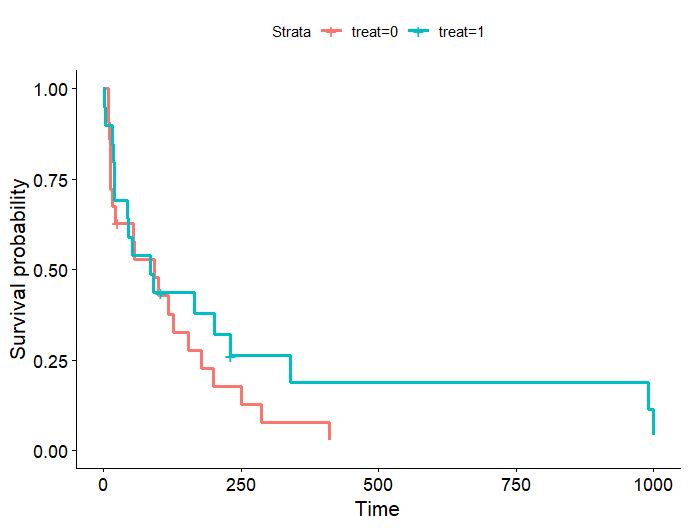
\includegraphics[width=.72\linewidth]{assets/lung_survival.png}\end{center}

\textbf{（2）} 用病理类型1作参照，令 \(I_k=I(type=k)\)： \[\begin{aligned}
h(t\mid X)=h_0(t)\exp\{&-0.614treat-0.001age+0.017coursetime\\&+0.488I_2+1.683I_3+0.264I_4\}.
\end{aligned}\]

\begin{longtable}[]{@{}lrrrl@{}}
\toprule\noalign{}
变量 & \(\beta\) & SE & \(P\) & HR（95\% CI） \\
\midrule\noalign{}
\endhead
\bottomrule\noalign{}
\endlastfoot
试验疗法 & −0.614 & 0.408 & 0.132 & 0.541 (0.244--1.203) \\
年龄 & −0.001 & 0.019 & 0.969 & 0.999 (0.963--1.037) \\
病程 & 0.017 & 0.013 & 0.179 & 1.017 (0.992--1.043) \\
类型2 vs 1 & 0.488 & 0.532 & 0.358 & 1.630 (0.575--4.619) \\
类型3 vs 1 & 1.683 & 0.615 & 0.006 & 5.384 (1.614--17.963) \\
类型4 vs 1 & 0.264 & 0.470 & 0.574 & 1.302 (0.518--3.273) \\
\end{longtable}

\textbf{（3）} 全模型中类型3与类型1的对比有统计学意义。但分类变量整体检验与单个哑变量检验不同，不能直接删除所有不显著项后沿用原系数，声称得到``最终模型''。研究关心的治疗因素应保留。

\textbf{（4）} PH诊断：治疗项Schoenfeld检验 \(P=0.75\)，全局 \(P=0.42\)，未发现显著违反PH的证据。曲线相交只是提示；\(P>0.05\) 不是证明假定成立。全模型似然比9.96（6自由度，\(P\approx0.13\)）、Wald10.28、Score11.23（原稿均约0.1、0.1、0.08）。\(C=0.638\) 表示区分能力有限，C指数不是完整的拟合/校准指标，亦非只在0.5--1之间取值。进一步检查函数形式、影响点、校准与内部验证。

\textbf{（5）} 调整后试验疗法的死亡瞬时风险点估计较低，但区间跨1，未能证实疗效差异；不等于两种疗法等效。可能原因包括样本小、估计不精确、残余混杂或真实差异较小。解释病理类型时明确参照，不能把类型编码直接乘以哑变量系数。


\Answer{H3-2}{hsCRP与死亡风险：文献分析}

\textbf{科学问题。} 可疑急性冠脉综合征患者中，肌钙蛋白之外，轻度升高的hsCRP是否与短期和长期全因死亡相关，并改善预测？

\textbf{变量。} 人口学：出生年份/年龄、性别、种族；临床：首次测量血红蛋白、白细胞、血小板、肌酐、肌钙蛋白、hsCRP等连续指标，以及ICD诊断等分类指标；身份标识：脱敏NHS号、医院号；结局：时间起点、死亡/随访结束时间、死亡状态。\textbf{原稿``死亡日期转换为当日生存率''不准确：个体原始结局应为随访时间和事件指示，生存率是群体估计量。}

\textbf{设计与分析。} 回顾性队列。原评分稿记述5家英国心血管中心源人群257,948人，分析102,337人，中位随访3.3年。hsCRP分为 \(<2\)、2--4.9、5--9.9、10--15 mg/L，以 \(<2\) 为参照。多变量Cox模型估计30天和3年死亡关联的HR及95\% CI。模型1调整年龄、性别、血红蛋白、肌酐；模型2再加肌钙蛋白；模型3再加hsCRP。

原文对PH不成立采用分时段效应：\(<1\)、1--3、3--6、6--12、12--24、24--36个月；连续变量可用限制性立方样条处理非线性。比较区分度、AUROC、NRI、IDI和阴性预测值时，应按原文处理删失与预测时间窗。模型和变量要对应到研究问题，不能只翻译摘要。


\subsection{往年题}

\Answer{R24-M13}{乘积极限法的计算}

\textbf{答案：C。}

条件生存概率连乘：\(\widehat S=(1-2/5)(1-1/3)=\frac35\times\frac23=0.40\)。

\textbf{补写说明。} 原稿第13题整题缺失；本题为新编练习，并非恢复的往年原题。


\Answer{R24-M4}{事件与删失的排序}

\textbf{答案：A。}

A项错误。同一记录时点同时有事件和右删失时，常规KM约定先计事件，后移除删失者；在事件时刻的风险集中包含同刻删失者。

\textbf{补写说明。} 原稿只记一个错误选项，其内容保留为A；提问句及B---E为补写。


\Answer{R24-M5}{生存曲线检验的权重}

\textbf{答案：B。}

按课程相对比较口径，通常选 \textbf{B}：Breslow以风险集人数加权，相对更强调早期；Log-rank相对于Breslow对后期差异保留更多权重。严格地说，不能保证Log-rank总对任意``远期效应''最敏感；其效能取决于生存差异形式，PH下表现良好。

\textbf{补写说明。} 原有五个选项保留；提问句根据回忆内容补全。此处``远期''是相对于Breslow的课程比较。


\Answer{R24-M6}{比例风险与时间}

\textbf{答案：D。}

根据本题已明确的个体风险函数，在共同基线、PH成立且比较的协变量不随时间变化时，\(h(t\mid x_a)/h(t\mid x_b)=\exp\{\beta^T(x_a-x_b)\}\)，与时间无关。若严格指同一模型的共同基线风险函数，其比值就是1。分层Cox不同层基线可不同，不能套用同一结论。

\textbf{补写说明。} 原稿未记选项，并写作``基线风险函数之比''；此处按通常考点将提问对象明确为个体风险函数。


\Answer{R24-M10}{删失与终点事件}

\textbf{答案：A。}

研究终点为肝癌死亡时，\textbf{A}为观察到的事件。B、E属于竞争事件；在原因别风险分析的传统编码中常在竞争死亡时删失，但估计肝癌累计发生概率时需要竞争风险方法。若研究终点为全因死亡，分类会不同。

\textbf{补写说明。} 题干明确了肝癌死亡终点，五个选项保留。


\Answer{R24-D3}{比例风险假设}

固定协变量的两个个体，其风险函数之比不随时间改变：\(HR=\exp\{\beta^T(x_a-x_b)\}\)。允许共同的基线风险 \(h_0(t)\) 随时间变化，并不要求每个人的风险本身恒定。


\Answer{R24-D4}{删失数据}

事件时间只被部分观察到的数据。右删失知道事件时间大于最后观察时间；左删失知道小于某时间；区间删失知道落在某区间。随访结束未发生事件、失访可产生右删失。常规生存估计需适当的非信息性删失假定。


\Answer{Z-D4}{删失数据／截尾数据（Censored data）}

事件时间只获得部分信息。原汇总给的是右删失定义：只知道真实事件时间超过最后观察时间。更一般还包括左删失和区间删失。


\Answer{Z-D5}{比例风险假设（PH Assumption）}

固定协变量个体间的HR不随时间改变；基线风险本身可随时间变化。


\Answer{Z-D6}{风险比（Hazard Ratio, HR）}

同一时刻两种条件下瞬时风险函数之比。Cox模型在PH成立时 \(HR=e^{\beta^T\Delta x}\)；HR不等于累计风险比或OR。


\Answer{R24-S1}{乘积极限法}

有个体事件/删失时间的未分组资料可采用Kaplan--Meier法，不限于小样本。将每个不同事件时刻视为分割点，按条件生存概率连乘： \[\hat S(t)=\prod_{t_i\le t}\left(1-\frac{d_i}{n_i}\right),\] 其中 \(n_i\) 为事件前风险人数，\(d_i\) 为该时刻事件数。可充分利用删失前的信息，不需指定生存时间分布，也不需人为分组；尾部风险人数很少时不稳定，应展示风险人数和区间。


\Answer{R24-S3}{Cox系数与用途}

其他协变量固定、PH成立时，\(X_j\) 增加1单位，瞬时风险乘以 \(e^{\beta_j}\)；\(\beta_j\) 为对应HR的自然对数。分类变量相对参照水平解释，交互项存在时需条件化。用于分析生存时间的关联因素、调整混杂、比较治疗/暴露，以及在模型验证和基线风险估计后预测生存概率。


\Answer{Z-S3}{删失的常见原因}

右删失表示只知道事件时间晚于观察截止。例：随访结束未发生事件、随访期间失访、以特定死因为终点时发生其他死因死亡。第三种同时涉及竞争风险，分析需与目标估计量一致。


\Answer{Z-S4}{KM法与寿命表法}

KM法适用于掌握个体事件/删失时间的原始资料，以每个事件时刻划分风险集，大小样本均可。寿命表法适用于按时间区间汇总的资料，通常需区间内删失分布的近似。原汇编只强调``小样本/大样本''过于简化，关键在记录精度和分组形式。


\Answer{Z-S5}{两种生存曲线检验}

二者比较各组生存经验中的观察/期望事件差异，通常以生存分布相同为无效假设。Log-rank对各事件时刻采用常规等权的观察减期望贡献；Breslow广义Wilcoxon用风险集人数加权，更强调早期。原汇编``Log-rank对远期更敏感''应理解为相对Breslow的课程表述，非普遍定律。


\Answer{Z-S6}{PH假设及其评价}

HR不随时间改变。可看对数负对数生存曲线是否大致平行、检验/绘制缩放Schoenfeld残差，以及检验协变量与时间交互。需同时关注每个变量与全局检验；未拒绝PH不等于证明PH。


\Answer{E19-2}{删失、非比例风险与交互作用}

``截尾''在本课程语境中指删失，即事件时间只有部分信息，右删失时知道 \(T>C\)。严格术语中 truncation（截断）涉及样本被观察到的选择机制，与 censoring不同。

PH不成立可考虑时变系数（协变量与时间交互）、分时段效应、对不关注其系数的变量分层，或根据科学问题改用其他生存模型。应先核对函数形式、异常点及诊断证据。

同时吸烟饮酒与均不者相比，\(HR=e^{0.693+1.099+0.405}\approx9\)；饮酒者中吸烟与不吸烟相比，\(HR=e^{0.693+0.405}\approx3\)。原表写RR，但Cox的指数系数应解释为瞬时风险比HR，不是累计发病概率之比。


\Answer{R24-C2}{心肌梗死风险因素的性别差异}

可能使用Cox比例风险模型，以随访时间和心肌梗死事件指示共同构成生存结局；可处理右删失，无需指定基线风险函数的参数形式，但须检查PH等前提。仅凭HR标签不能排除其他生存模型，应与文献方法核对。

按男女分别报告HR、95\% CI、参照及调整变量。判断性别差异应用性别\(\times\)因素交互作用或等价异质性检验；``男性显著、女性不显著''不等于两者效应差异显著。原图缺失，不能补造具体结论。


\Answer{E19-4}{戒毒方式与复吸时间}

\textbf{整理者复算。} 以 \((time,censor)\) 构成生存结局，模型纳入treat、age、ndrugtx、site、herco；site、herco按分类变量处理。628条原始记录，完整记录610条，495次复吸。长期相对短期：\(\hat\beta=-0.2546\)，HR=0.7752，95\% CI 0.6486--0.9266，\(P=0.00515\)。调整其他变量后，长期方案与较低的复吸瞬时风险相关。

年龄每增1岁HR=0.9765；既往戒毒每增1次HR=1.0354。herco=2相对1的HR=1.2806（\(P=0.0439\)）；site与herco=3对比未达到0.05水平。PH全局检验 \(P=0.318\)，治疗项 \(P=0.092\)，未发现明显违反证据；仍应观察残差图。模型 \(C=0.581\)，预测区分度有限。不要将名为censor的列再次反转编码。


\Answer{E20-3}{冠心病数据分析（2020）}

\textbf{先明确结局。} 原数据的Status只有Alive/Dead，没有死亡原因。因此不能从现有数据直接识别``冠心病特异死亡''。原材料将已确诊冠心病的1449人留下，按确诊后生存时间建模，实际得到的是\textbf{冠心病确诊者后续全因死亡}的分析，不等同于原题的病因特异结局。

\textbf{可复现的示范。} 明示把随访结束近似为基线后32年，确诊者中死亡者时间为``死亡年龄减确诊年龄''，存活者时间为 \(32-(AgeCHDdiag-AgeAtStart)\)。该时间近似用于复现教学分析；若需精确分析，应补齐日期。使用确诊年龄、性别、体重状态、吸烟状态、血压状态、胆固醇状态的Cox模型，参照组为女性、正常体重、不吸烟、理想血压、适宜胆固醇。两年原始表排序不同，但本设定复算均为1405条完整记录、865个死亡事件。

报告系数、HR、95\% CI、PH和共线性诊断；R程序随包提供。原答卷的年龄HR约1.07、男性约1.67、高血压约1.77属于上述全因死亡示例，不能挪作冠心病特异死亡结果。原答卷``偏瘦HR=1.31''与其表中1.98不符；表中BP的PH检验 \(P=0.040\) 也不能被全局 \(P=0.07\) 掩盖。

\textbf{若严格回答原题。} 需要死因或可靠冠心病死亡标志，之后构造病因特异事件、明确竞争事件处理；如果目标是从基线开始的风险分析，亦不能事后仅保留最终确诊者而改变目标人群。


\Answer{E21-3}{冠心病数据分析（2021）}

\textbf{先明确结局。} 原数据的Status只有Alive/Dead，没有死亡原因。因此不能从现有数据直接识别``冠心病特异死亡''。原材料将已确诊冠心病的1449人留下，按确诊后生存时间建模，实际得到的是\textbf{冠心病确诊者后续全因死亡}的分析，不等同于原题的病因特异结局。

\textbf{可复现的示范。} 明示把随访结束近似为基线后32年，确诊者中死亡者时间为``死亡年龄减确诊年龄''，存活者时间为 \(32-(AgeCHDdiag-AgeAtStart)\)。该时间近似用于复现教学分析；若需精确分析，应补齐日期。使用确诊年龄、性别、体重状态、吸烟状态、血压状态、胆固醇状态的Cox模型，参照组为女性、正常体重、不吸烟、理想血压、适宜胆固醇。两年原始表排序不同，但本设定复算均为1405条完整记录、865个死亡事件。

报告系数、HR、95\% CI、PH和共线性诊断；R程序随包提供。原答卷的年龄HR约1.07、男性约1.67、高血压约1.77属于上述全因死亡示例，不能挪作冠心病特异死亡结果。原答卷``偏瘦HR=1.31''与其表中1.98不符；表中BP的PH检验 \(P=0.040\) 也不能被全局 \(P=0.07\) 掩盖。

\textbf{若严格回答原题。} 需要死因或可靠冠心病死亡标志，之后构造病因特异事件、明确竞争事件处理；如果目标是从基线开始的风险分析，亦不能事后仅保留最终确诊者而改变目标人群。


\subsection{补充练习}

\Answer{P3-M1}{时段生存概率与累计生存率}

\textbf{答案：C。} 因为\(\{T>5\}\subset\{T>2\}\)，
\[P(T>5\mid T>2)=\frac{S(5)}{S(2)}=0.75.\]
这是已生存满2年者继续生存至5年的条件概率。\(F(5)=1-S(5)=0.40\)；瞬时风险\(h(5)\)不是\(1-S(5)\)，仅凭两个生存率不能确定。



\Answer{P3-D1}{中位生存期}

中位生存期是生存分布的第50百分位数，即生存函数降至0.5所对应的时间。对阶梯状KM估计，取\(\inf\{t:\hat S(t)\le0.5\}\)，即首次降至0.5或以下的事件时刻。若随访内未降至0.5，应报告“中位生存期尚未达到／在本观察期内不可估计”，不能用最长随访时间或死亡者生存时间的中位数代替。寿命表的分组估计可按正文作线性内插。



\Answer{P3-S1}{删失者如何参与部分似然}

说法错误。删失者在删失之前仍在风险集中，会参与此前事件时刻的分母。

时刻1前，风险集为\(\{\text{甲、乙、丙、丁}\}\)；时刻3前，甲已发生事件、乙已删失，风险集为\(\{\text{丙、丁}\}\)。没有并列事件，故
\[L_p(\beta)=\frac{1}{2+2e^\beta}\times\frac{e^\beta}{1+e^\beta}.\]
例如\(\beta=0\)时，两个贡献为\(1/4\)、\(1/2\)，乘积为\(1/8\)。乙、丁虽没有独立的事件分子，仍提供有效信息。

在同一时刻给定风险集中有人发生事件，某个体的贡献为\(h_i(t)/\sum_{l\in R(t)}h_l(t)\)。各人的共同因子\(h_0(t)\)约去，从而只剩协变量与\(\beta\)。



\Answer{P3-C1}{有并列时间的KM计算}

\textbf{（1）} 事件时刻只有1、2、4月：
\begin{center}\begin{tabular}{rrrr}\toprule
\(t_i\) & \(n_i\) & \(d_i\) & \(\hat S(t_i)\)\\\midrule
1 & 8 & 1 & \(7/8=0.875\)\\
2 & 7 & 1 & \((7/8)(6/7)=0.750\)\\
4 & 4 & 2 & \((3/4)(2/4)=0.375\)\\\bottomrule
\end{tabular}\end{center}
2月的风险集包含同刻删失者；2月后余5人，3月再删失1人，所以4月前余4人。

\textbf{（2）} \(\hat S(3)=0.750\)、\(\hat S(4)=0.375\)。首次降至0.5以下为4月，中位生存期为4月。删失不会直接使曲线下降，而会改变之后的风险人数；5、6月的删失也不会把末尾生存率降为0。

\textbf{（3）}
\[SE\{\hat S(4)\}=0.375\sqrt{\frac1{8\times7}+\frac1{7\times6}
+\frac2{4\times2}}=0.2025.\]
不能把已删失者一开始就剔除，也不能在2月先移除删失者再计算死亡概率。



\Answer{P3-C2}{寿命表与中位生存期的内插}

\textbf{（1）} 有效人数为\(n_i=n_i'-c_i/2\)，条件生存概率为\(p_i=1-d_i/n_i\)：
\begin{center}\begin{tabular}{lrrr}\toprule
区间 & 有效人数 & \(p_i\) & 区间末\(\hat S\)\\\midrule
0--1 & 90 & 0.80 & 0.80\\
1--2 & 50 & 0.80 & 0.64\\
2--3 & 28 & 0.75 & 0.48\\\bottomrule
\end{tabular}\end{center}
期初人数递推也自洽：\(100-18-20=62\)，\(62-10-24=28\)。

\textbf{（2）} 0.5位于2年和3年的生存率之间，内插为
\[\hat t_{0.5}=2+\frac{0.64-0.50}{0.64-0.48}(3-2)=2.875\text{年}.\]
这是分组资料下的近似，不能当作精确事件时刻。

\textbf{（3）} 0.75的条件是已经生存至第3个区间开始，而3年生存率须累乘前面各区间，得到\(0.8\times0.8\times0.75=0.48\)。原表缺少区间内事件、删失的确切时间与顺序，不能唯一还原KM曲线。



\Answer{P3-C3}{从预后指数计算生存率}

\textbf{（1）} 基线对应50岁、标准疗法。60岁试验组患者有
\[PI=\log0.5+\log1.5=\log0.75=-0.2877,\quad HR=e^{PI}=0.75.\]
年龄是按每10岁进入方程，不能把60直接乘以年龄系数。

\textbf{（2）} 由正文公式\(\hat S(t\mid X)=\hat S_0(t)^{e^{PI}}\)，得
\[\hat S(3\mid X)=0.64^{0.75}=0.7155.\]
HR作用于风险函数；在生存函数中进入\textbf{指数}，不能计算成\(0.64\times0.75\)。

\textbf{（3）} 相同年龄比较两疗法，\(HR=0.5\)。60岁标准组的3年生存率为\(0.64^{1.5}=0.512\)，故本例3年累计死亡概率之比为
\[\frac{1-0.7155}{1-0.512}\approx0.5829,\]
与0.5不同。HR是同一时刻瞬时风险之比，不是指定随访期限的累计死亡概率之比。



\Answer{P3-L1}{体育活动、死亡终点与剂量反应}

\textbf{（1）} 个体结局由随访时间与事件指示共同构成。时间从规定基线至死亡、失访或随访截止；以全因死亡为终点，癌症死亡也记事件1，而非删失0。换成死因别终点时需重新定义事件及其他死因的处理。

\textbf{（2）} 在模型调整因素相同并满足其假定时，75--149分钟/周组全因死亡瞬时风险为参照组的0.81倍，即相对低19\%；95\% CI为0.76--0.87，未跨1。心血管疾病死亡的HR为0.69，即相应瞬时风险低31\%，95\% CI为0.60--0.78。它们不表示30年死亡概率下降相同的百分点，也不能仅凭观察性关联断言运动干预造成同样幅度的下降。

\textbf{（3）} 限制性立方样条用于描述连续运动时长与对数风险之间可能的\textbf{非线性剂量反应关系}。PH关注效应是否随随访时间变化，是另一项问题，仍需另行评价。高运动量端趋平提示增加运动时长的额外关联可能减弱；还应结合置信区间和该段数据量，不能只凭曲线宣布某一剂量绝对最优。
\EndExercises

\chapter{对数线性模型}
\sourcepages{7}{1-6}
logistic回归与Cox回归均区分结局变量与自变量。对数线性模型分析多个分类变量交叉构成的列联表，各变量地位相同，研究目的是描述变量间的关联结构，即哪些变量之间存在关联，以及这种关联在第三个变量的不同水平上是否相同。

对数线性模型将各格频数视为Poisson变量，将期望频数的对数表示为各变量主效应与交互项之和。两个变量相互独立对应于模型中不含二者的交互项，变量间关系的判断由此转化为一系列嵌套模型偏差的比较。本章要求能够将模型中的交互项转换为关联结构，例如含$u_{12}$、$u_{13}$而不含$u_{23}$，表示给定变量1时变量2与变量3条件独立。

本章开头的辛普森悖论表明，将多维列联表随意合并为二维表进行$\chi^2$检验，结论可能完全相反。
\section{问题提出}
\textbf{例1} 宫颈癌。变量包括肤色、收入、分娩次数。
\ctable{表1\quad 宫颈癌患病情况}{\begin{tabular}{llrrr}\toprule 肤色&家庭收入&少（0--1次）&中等（2--3次）&多（4次及以上）\\\midrule
白人&低收入&67&143&43\\
&中收入&36&78&16\\
&高收入&3&9&12\\
有色人种&低收入&77&94&25\\
&中收入&87&70&18\\
&高收入&14&8&14\\\bottomrule\end{tabular}}
常见的数据整理方式：合并、压缩维度。
\ctable{按肤色列表（合并收入后：肤色$\times$分娩次数）}{\begin{tabular}{lrrr}\toprule 肤色&少（0--1次）&中等（2--3次）&多（4次及以上）\\\midrule
白人&106$^*$&230&71\\
有色人种&178&172&57\\\bottomrule\end{tabular}}\ctable{按收入列表（合并肤色后：收入$\times$分娩次数）}{\begin{tabular}{lrrr}\toprule 家庭收入&少（0--1次）&中等（2--3次）&多（4次及以上）\\\midrule
低收入&144&237&68\\
中收入&123&148&34\\
高收入&17&17&26\\\bottomrule\end{tabular}\par\smallskip\footnotesize $^*$原表印作160；$67+36+3=106$，白人合计 $106+230+71=407$，与有色人种合计407相同。第一个表的行变量是肤色，原表头误作“家庭收入”。}
采用 $\chi^2$ 检验对上述 $R\times C$ 列联表分析任意两因素之间的关系，做法正确吗？混杂因素？
\subsection{辛普森悖论（Simpson's paradox）}
\sourcepages{7}{7-10}
将高维列联表压缩为多个二维列联表进行分析时候，可能会出现奇怪的结果。
\ctable{给定C的情况下，A与B之间存在正相关关系}{\begin{minipage}{.45\linewidth}\centering\begin{tabular}{lrr}\toprule $C_1$&$B_1$&$B_2$\\\midrule $A_1$&60&80\\ $A_2$&60&90\\\bottomrule\end{tabular}\par\smallskip $\widehat{\OR}=1.13$\end{minipage}\hfill\begin{minipage}{.45\linewidth}\centering\begin{tabular}{lrr}\toprule $C_2$&$B_1$&$B_2$\\\midrule $A_1$&60&220\\ $A_2$&30&120\\\bottomrule\end{tabular}\par\smallskip $\widehat{\OR}=1.09$\end{minipage}\par\medskip\begin{minipage}{.45\linewidth}\centering\begin{tabular}{lrr}\toprule $C_3$&$B_1$&$B_2$\\\midrule $A_1$&40&170\\ $A_2$&60&270\\\bottomrule\end{tabular}\par\smallskip $\widehat{\OR}=1.06$\end{minipage}\hfill\begin{minipage}{.45\linewidth}\centering\begin{tabular}{lrr}\toprule $C_4$&$B_1$&$B_2$\\\midrule $A_1$&40&430\\ $A_2$&30&330\\\bottomrule\end{tabular}\par\smallskip $\widehat{\OR}=1.02$\end{minipage}}\ctable{合并C的两个类别之后，A与B存在负相关关系}{\begin{minipage}{.45\linewidth}\centering\begin{tabular}{lrr}\toprule $C_1+C_2$&$B_1$&$B_2$\\\midrule $A_1$&120&300\\ $A_2$&90&210\\\bottomrule\end{tabular}\par\smallskip $\widehat{\OR}=0.93$\end{minipage}\hfill\begin{minipage}{.45\linewidth}\centering\begin{tabular}{lrr}\toprule $C_3+C_4$&$B_1$&$B_2$\\\midrule $A_1$&80&600\\ $A_2$&90&600\\\bottomrule\end{tabular}\par\smallskip $\widehat{\OR}=0.89$\end{minipage}}\ctable{合并C的所有类别之后，A与B不存在相关关系}{\begin{minipage}{.45\linewidth}\centering\begin{tabular}{lrr}\toprule $C_1+C_2+C_3+C_4$&$B_1$&$B_2$\\\midrule $A_1$&200&900\\ $A_2$&180&810\\\bottomrule\end{tabular}\par\smallskip $\widehat{\OR}=1.0$\end{minipage}}
\begin{annotation}研究A和B的关系，C因素有4个层次，分层分析结果显示A和B正相关。研究A和B的关系，将C因素合并为仅有2个层次，分层分析结果变为A和B负相关。\end{annotation}
\sourcepages{7}{11-13}
\textbf{例2：癌症数据} 生存状态（A）：$A_1=$死亡，$A_2=$存活；治疗方案（B）：$B_1=$常规疗法，$B_2=$新疗法。
\ctable{重症 $C_1$}{\begin{tabular}{lrrr}\toprule $C_1$&$B_1$&$B_2$&合计\\\midrule
$A_1$&950&9000&9950\\
$A_2$&50&1000&1050\\
合计&1000&10000&11000\\\bottomrule\end{tabular}}\[P(A_2\mid B_1)=0.05,\qquad P(A_2\mid B_2)=0.10.\]\ctable{非重症 $C_2$}{\begin{tabular}{lrrr}\toprule $C_2$&$B_1$&$B_2$&合计\\\midrule
$A_1$&5000&5&5005\\
$A_2$&5000&95&5095\\
合计&10000&100&10100\\\bottomrule\end{tabular}}\[P(A_2\mid B_1)=0.50,\qquad P(A_2\mid B_2)=0.95.\]\ctable{合并重症与非重症}{\begin{tabular}{lrrr}\toprule $C_1+C_2$&$B_1$&$B_2$&合计\\\midrule
$A_1$&5950&9005$^*$&14955$^*$\\
$A_2$&5050&1095&6145\\
合计&11000&10100&21100\\\bottomrule\end{tabular}}\[P(A_2\mid B_1)=0.46,\qquad P(A_2\mid B_2)=0.11.\]
{\footnotesize $^*$原表印作9050、14995；按 $9000+5=9005$、$5950+9005=14955$ 更正（列合计10100、总计21100不变）。}
新的治疗方案和普通治疗方案均更适合“非重症”的癌症病人。
\begin{annotation}以及无论对重症还是非重症都是新疗法好。分布不均！主要是重症患者用新疗法，即便新疗法好，本身重症就风险更大。\end{annotation}
合并后，似乎新的治疗方案效果较普通治疗方案更差。为什么？
\[
\text{对 }B_1\text{ 而言，重症:非重症}=1000:10000,
\]
\[
\text{对 }B_2\text{ 而言，重症:非重症}=10000:100.
\]
两变量间相关关系的大小和方向可能取决于它们与第三个变量间的相关关系——第三个变量为混杂因素。
\begin{sikao}[辛普森悖论的模型分析]
将癌症数据整理为$2\times2\times2$频数表，分别估计未调整与调整病情时新疗法的存活OR：
\par\noindent
\begin{coursecode}{R}
ca <- expand.grid(A=c("死亡","存活"), B=c("常规","新"), C=c("重症","非重症"))
ca$n <- c(950,50,9000,1000, 5000,5000,5,95)
w  <- reshape(ca, idvar=c("B","C"), timevar="A", direction="wide")   # 改成宽格式
lc <- glm(cbind(n.存活,n.死亡)~B,   binomial, w)    # 不调整病情
lg <- glm(cbind(n.存活,n.死亡)~B+C, binomial, w)    # 调整病情
exp(coef(lc)["B新"]); exp(coef(lg)["B新"])
ll <- glm(n~A*B + A*C + B*C, poisson, ca)          # 无三阶交互的对数线性模型
coef(ll)[c("A存活:B新","A存活:C非重症")]; coef(lg)[c("B新","C非重症")]
\end{coursecode}
\begin{routput}
      B新 
0.1432702 
    B新 
3.38963
    A存活:B新 A存活:C非重症 
     1.220721      3.405542 
     B新  C非重症 
1.220721 3.405542 
\end{routput}
未调整病情时，新疗法存活的OR仅为0.14；调整病情后OR为3.39，即在病情相同的患者中新疗法的效果明显较好。其原因在于新疗法主要用于重症患者（10000:100），而重症患者本身存活率较低。

输出的后两行表明：以生存状态A为结局的logistic回归\texttt{A\textasciitilde B+C}，与含$AB$、$AC$、$BC$三个交互项的对数线性模型给出相同的系数。对数线性模型中$A$与$B$的交互项即logistic回归中$B$的对数OR，$BC$项相当于对自变量间的关联不加限制。因此，列联表中有一个变量为结局时，对数线性模型与logistic回归等价，后者更为直接；各变量地位相同、关注整体关联结构时，宜采用对数线性模型。
\end{sikao}
\subsection{学习要点}
\sourcepages{7}{14}
\begin{enumerate}
\item 什么是高维列联表。
\item 将一个高维列联表转换为多个二维列联表，并对每个二维列联表采用 $\chi^2$ 检验进行分析的做法并不总是合适的。
\item 什么是对数线性模型，如何解释模型结果。
\item 分类变量何时可以合并处理，何时不能。
\end{enumerate}
\section{对数线性模型}
\sourcepages{7}{15}
对数线性模型（Log-linear model）通常用于分析高维列联表数据。
\begin{enumerate}
\item 描述和确定高维列联表中分类变量间的相关关系。
\item 可在不歪曲变量间相关关系的情况下探讨合并列表数据的可能性。
\end{enumerate}
\subsection{四格表资料的对数线性模型}
\sourcepages{7}{16-19}
\ctable{四格表的频数与概率}{\begin{tabular}{lccc}\toprule
&$B_1$&$B_2$&合计\\\midrule
$A_1$&$n_{11}$&$n_{12}$&$n_{1\cdot}$\\
$A_2$&$n_{21}$&$n_{22}$&$n_{2\cdot}$\\
合计&$n_{\cdot1}$&$n_{\cdot2}$&$n_{\cdot\cdot}$\\\bottomrule\end{tabular}\qquad
\begin{tabular}{lccc}\toprule
&$B_1$&$B_2$&合计\\\midrule
$A_1$&$p_{11}$&$p_{12}$&$p_{1\cdot}$\\
$A_2$&$p_{21}$&$p_{22}$&$p_{2\cdot}$\\
合计&$p_{\cdot1}$&$p_{\cdot2}$&1\\\bottomrule\end{tabular}}
\begin{annotation}$n_{ij}$ 为观察频数，$p_{ij}$ 为格子概率；下标中的“$\cdot$”表示对该下标求和，$n_{i\cdot}$、$p_{i\cdot}$ 为行合计，$n_{\cdot j}$、$p_{\cdot j}$ 为列合计。$i$ 是第一个变量（A）的第 $i$ 个水平，$j$ 是第二个变量（B）的第 $j$ 个水平。\end{annotation}
\textbf{三种抽样方式}\quad 同一张四格表可以来自不同的抽样：
\begin{itemize}
\item \textbf{独立Poisson抽样}：观察一段时间，各格频数 $n_{ij}\sim\text{Poisson}(\mu_{ij})$ 相互独立，总数不固定；
\item \textbf{多项抽样}：固定总样本量 $n$，每人独立落入4个格子之一，各格频数服从多项分布 $\text{Multinomial}(n;\,p_{11},\ldots,p_{22})$；
\item \textbf{乘积多项抽样}：固定行合计（如按暴露分组抽样）或列合计（如病例对照），每行（列）内部是独立的多项（二项）分布。
\end{itemize}
\begin{derivation}{独立Poisson频数给定总数后服从多项分布}
\dpart{假设}$N_c\sim\text{Poisson}(\mu_c)$，$c=1,\ldots,C$ 相互独立，$\mu=\sum_c\mu_c$。
\dpart{关键等式}独立Poisson变量之和仍服从Poisson分布，$N=\sum_cN_c\sim\text{Poisson}(\mu)$。对 $\sum_cn_c=n$，
\[
P(N_1=n_1,\ldots,N_C=n_C\mid N=n)
=\frac{\prod_c e^{-\mu_c}\mu_c^{n_c}/n_c!}{e^{-\mu}\mu^n/n!}
=\frac{n!}{\prod_cn_c!}\prod_c\Bigl(\frac{\mu_c}{\mu}\Bigr)^{n_c}.
\]
\dpart{结论}给定总数后，频数服从多项分布，格子概率 $p_c=\mu_c/\mu$。
\dpart{解释}Poisson似然可分解为“总数 $N$ 的Poisson似然”乘“给定 $N$ 的多项似然”，且只要模型含常数项 $u$，前者只与 $\mu$ 有关。因此用Poisson对数线性模型（含常数项）得到的关联参数估计和拟合优度统计量，与多项抽样下完全相同；乘积多项抽样下，只要模型包含被固定边际对应的项（如固定行合计时含 $u_1$），结论也相同。这是可以统一用Poisson GLM拟合列联表的理由。
\end{derivation}
\textbf{对数线性模型的分解}\quad 记期望频数 $F_{ij}=np_{ij}$。常见的写法是
\begin{align*}
F_{ij}&=np_{ij}=n\frac{p_{i\cdot}p_{\cdot j}}{p_{i\cdot}p_{\cdot j}}p_{ij}
=np_{i\cdot}p_{\cdot j}\frac{p_{ij}}{p_{i\cdot}p_{\cdot j}},\\
\ln F_{ij}&=\ln n+\ln p_{i\cdot}+\ln p_{\cdot j}
+\ln\frac{p_{ij}}{p_{i\cdot}p_{\cdot j}}.
\end{align*}
这个恒等式说明了 $\ln F_{ij}$ 可分为“样本量、A的边际、B的边际、A与B的关联”四部分，但不能直接令 $u_1(i)=\ln p_{i\cdot}$ 等，因为 $\ln p_{i\cdot}$ 之和不为0（各项都为负），不满足下面的零和约束；$\ln\{p_{ij}/(p_{i\cdot}p_{\cdot j})\}$ 对 $i$ 或 $j$ 求和一般也不为0。正确的定义是对 $\ln F_{ij}$ 作“均值分解”（类似两因素方差分析）：
\begin{align*}
\ln F_{ij}&=u+u_1(i)+u_2(j)+u_{12}(ij),\\
u&=\overline{\ln F}_{\cdot\cdot},\quad
u_1(i)=\overline{\ln F}_{i\cdot}-\overline{\ln F}_{\cdot\cdot},\quad
u_2(j)=\overline{\ln F}_{\cdot j}-\overline{\ln F}_{\cdot\cdot},\\
u_{12}(ij)&=\ln F_{ij}-\overline{\ln F}_{i\cdot}-\overline{\ln F}_{\cdot j}+\overline{\ln F}_{\cdot\cdot},
\end{align*}
其中 $\overline{\ln F}_{i\cdot}$ 为第 $i$ 行 $\ln F_{ij}$ 的算术均数，其余类推。$2\times2$ 表中 $u_{12}(11)=\tfrac14\ln\dfrac{F_{11}F_{22}}{F_{12}F_{21}}=\tfrac14\ln\OR$，$u_{12}=0$ 当且仅当 $\OR=1$，即A与B独立。
\begin{annotation}理论频数由样本量（常数项）、A变量、B变量、A和B交互作用决定。\end{annotation}
\[
\sum_i u_1(i)=\sum_j u_2(j)=0,\qquad
\sum_i u_{12}(i,j)=\sum_j u_{12}(i,j)=0.
\]
\textbf{约束与可识别性}\quad 不加约束时，$u$、$u_1(1),u_1(2)$、$u_2(1),u_2(2)$、$u_{12}(11),\ldots,u_{12}(22)$ 共9个参数只对应4个格子，可以互相加减常数而不改变 $F_{ij}$，参数不可识别。零和约束（或“参照水平取0”的约束，软件中更常用）使 $u_1$、$u_2$、$u_{12}$ 各只剩1个自由参数，加上 $u$ 共4个，与4个格子一一对应，即饱和模型。约束只是选定一种参数化，不影响拟合值和检验；但参数的数值与约束有关，解释参数时必须先说明用的是哪种约束。在多项抽样下总数 $n$ 固定，$u$ 由 $\sum F_{ij}=n$ 决定，固定总数的四格表只有3个自由的概率参数（如 $p_{11},p_{12},p_{21}$），分别对应 $u_1$、$u_2$、$u_{12}$。
\subsection{三维列联表的对数线性模型}
\sourcepages{7}{20-24}
$F_{ijk}$：格子 $(i,j,k)$ 的期望频数，其中 $i=1,\ldots,r$；$j=1,\ldots,c$；$k=1,\ldots,l$。（列合计）$\times$（行合计）/总数。
\subsubsection{饱和模型（Saturated model）}
\begin{align*}
\ln F_{ijk}={}&u+u_1(i)+u_2(j)+u_3(k)\\
&+\underbrace{u_{12}(i,j)+u_{13}(i,k)+u_{23}(j,k)}_{\text{一阶交互作用}}
+\underbrace{u_{123}(i,j,k)}_{\text{二阶交互作用}}.
\end{align*}
\begin{itemize}
\item $u$：$\ln F_{ijk}$ 的总体均值。
\item $u_1(i)$：变量1第 $i$ 级的主效应。
\item $u_2(j)$：变量2第 $j$ 级的主效应。
\item $u_3(k)$：变量3第 $k$ 级的主效应。
\end{itemize}
\[
\sum_i u_1(i)=\sum_j u_2(j)=\sum_k u_3(k)=0.
\]
$u_{12}(i,j)$：变量1第 $i$ 级与变量2第 $j$ 级的一阶交互效应。类似地，$u_{13}(i,k)$：变量1第 $i$ 级与变量3第 $k$ 级的一阶交互效应；$u_{23}(j,k)$：变量2第 $j$ 级与变量3第 $k$ 级的一阶交互效应。
\[
\sum_i u_{12}(i,j)=\sum_j u_{12}(i,j)=0.
\]
$u_{123}(i,j,k)$：变量1第 $i$ 级与变量2第 $j$ 级以及变量3第 $k$ 级的二阶交互效应。
\[
\sum_i u_{123}(i,j,k)=\sum_j u_{123}(i,j,k)=\sum_k u_{123}(i,j,k)=0.
\]
\begin{annotation}饱和模型包含所有主效应和各阶交互项，独立参数个数等于列联表的格子数。零和约束：任一交互项对它的任何一个下标求和都等于0。\end{annotation}
\textbf{注意} 对一个三维列联表拟合一个“饱和模型”会产生一系列的理论频数估计值。这些理论频数将会与观测频数完全一致。尽管此时模型完美拟合数据，也毫无意义。
\begin{annotation}这并非我们的目的。我们的目的是用最少的参数完成模型拟合，有些交互项可能可以删去。\end{annotation}
\subsubsection{层次模型（Hierarchical models）}
\sourcepages{7}{25-28}
\begin{annotation}嵌套：从饱和模型扣除最高阶交互，进行模型简化。条件独立模型、部分独立模型、互相独立模型。\end{annotation}
\textbf{1. 两两关联模型} 如果 $u_{123}=0$，则提示不存在二阶交互效应。
\[
\ln F_{ijk}=u+u_1(i)+u_2(j)+u_3(k)+u_{12}(i,j)+u_{23}(j,k)+u_{13}(i,k).
\]
其表明每一对变量均存在相关关系（两两关联模型，homogeneous association model）。

\textbf{2. 条件独立} 如果 $u_{123}=0$、$u_{12}=0$、$u_{23}\ne0$、$u_{13}\ne0$：
\[
\ln F_{ijk}=u+u_1(i)+u_2(j)+u_3(k)+u_{23}(j,k)+u_{13}(i,k).
\]
则表明变量1和变量2条件独立（Conditional Independence）。类似地，$u_{123}=0,u_{23}=0$，或 $u_{123}=0,u_{13}=0$，均为条件独立。
\begin{annotation}变量1与3、变量2与3都可以有关联，但在变量3的每一层内，变量1与2独立，故称“给定变量3时条件独立”，记作 $1\perp2\mid3$。此时把变量3合并后，1与2在边际表中一般仍会表现出关联（由它们共同与3相关所致）。\end{annotation}
\begin{derivation}{层次模型的约束与条件独立、同质关联}
\dpart{假设}三维表的格子概率 $p_{ijk}>0$，$F_{ijk}=np_{ijk}$。
\dpart{结论1}$u_{12}=u_{123}=0\iff$ 变量1与2在给定变量3时条件独立，即 $p_{ijk}=p_{i\cdot k}\,p_{\cdot jk}/p_{\cdot\cdot k}$。
\dpart{推导}($\Leftarrow$) 若条件独立，取对数 $\ln F_{ijk}=\ln n+\ln p_{i\cdot k}+\ln p_{\cdot jk}-\ln p_{\cdot\cdot k}$，右边是一个只含 $(i,k)$ 的函数加一个只含 $(j,k)$ 的函数，按均值分解后只会产生 $u,u_1,u_2,u_3,u_{13},u_{23}$ 项，不含 $u_{12}$、$u_{123}$。($\Rightarrow$) 若 $\ln F_{ijk}=a(i,k)+b(j,k)$，则 $F_{ijk}=A_{ik}B_{jk}$，于是在第 $k$ 层
\[
P(1=i,2=j\mid3=k)=\frac{A_{ik}B_{jk}}{\sum_{i'}A_{i'k}\sum_{j'}B_{j'k}}
=\frac{A_{ik}}{\sum_{i'}A_{i'k}}\cdot\frac{B_{jk}}{\sum_{j'}B_{j'k}},
\]
层内联合概率可分解为两个边际概率之积，即条件独立。
\dpart{结论2}$u_{123}=0\iff$ 各层的条件OR相同（同质关联）。以 $2\times2\times K$ 表为例，第 $k$ 层的条件对数OR
\[
\ln\OR_{12(k)}=\ln\frac{F_{11k}F_{22k}}{F_{12k}F_{21k}}=4u_{12}(11)+4u_{123}(11k),
\]
主效应和 $u_{13}$、$u_{23}$ 在这个交叉比中全部相消。故 $\OR_{12(k)}$ 不随 $k$ 变化 $\iff u_{123}(11k)$ 对所有 $k$ 相同；又 $\sum_ku_{123}=0$，即 $u_{123}\equiv0$。
\dpart{解释}两两关联模型（$u_{123}=0$）\emph{允许}每一对变量都有关联，只要求任一对变量的条件OR在第三个变量各层相同；它不强制关联存在，某个 $u_{12}$ 是否为0要由数据检验。模型从高阶交互项开始逐步删除，并保持层次性：含有某交互项时，必须同时含有它的所有低阶项。
\end{derivation}

\textbf{3. 部分独立} 如果 $u_{123}=0$、$u_{12}=u_{13}=0$、$u_{23}\ne0$：
\[
\ln F_{ijk}=u+u_1(i)+u_2(j)+u_3(k)+u_{23}(j,k).
\]
部分独立（Partial independence）。类似地，$u_{123}=0,u_{12}=u_{23}=0,u_{13}\ne0$；$u_{123}=0,u_{13}=u_{23}=0,u_{12}\ne0$。

\textbf{4. 相互独立} 如果 $u_{123}=u_{12}=u_{13}=u_{23}=0$：
\[
\ln F_{ijk}=u+u_1(i)+u_2(j)+u_3(k).
\]
相互独立（Mutual independence），或完全独立（Complete independence）。
\begin{annotation}只有主效应和常数项，没有任何交互作用。\end{annotation}
\cfigure{条件独立、部分独立与相互独立}{\begin{tikzpicture}[every node/.style={font=\small}]
\begin{scope}\draw[dashed] (0,0) ellipse (1.5 and 1);\node (c) at (-.7,0) {3};\node (a) at (.65,.5) {1};\node (b) at (.65,-.5) {2};\draw[PlotPrimary,line width=.65pt,-{Stealth}] (c)--(a);\draw[PlotPrimary,line width=.65pt,-{Stealth}] (c)--(b);\node at (0,-1.35) {条件独立};\end{scope}
\begin{scope}[xshift=4.5cm]\draw[dashed] (0,0) ellipse (1.5 and 1);\node at (0,.5) {1};\node (a) at (-.7,-.3) {2};\node (b) at (.7,-.3) {3};\draw[PlotPrimary,line width=.65pt,{Stealth}-{Stealth}] (a)--(b);\node at (0,-1.35) {部分独立};\end{scope}
\begin{scope}[xshift=9cm]\draw[dashed] (0,0) ellipse (1.5 and 1);\node at (0,.5) {1};\node at (-.7,-.3) {2};\node at (.7,-.3) {3};\node at (0,-1.35) {相互独立};\end{scope}
\end{tikzpicture}}
\sourcepages{7}{29-31}
\ctable{表2、表3\quad 对宫颈癌数据拟合所有层次模型的结果}{\begin{tabular}{llrrrrr}\toprule 模型&包含效应&df&LR卡方&$P$&Pearson卡方&$P$\\\midrule
完全独立&$u_1,u_2,u_3$&12&81.95&$<0.001$&91.31&$<0.001$\\
部分独立&$u_1,u_{23}$&8&46.01&$<0.001$&44.62&$<0.001$\\
&$u_2,u_{13}$&10&53.57&$<0.001$&62.19&$<0.001$\\
&$u_3,u_{12}$&10&65.62&$<0.001$&73.45&$<0.001$\\
条件独立&$u_{12},u_{13}$&8&37.24&$<0.001$&45.75&$<0.001$\\
&$u_{12},u_{23}$&6&29.67&$<0.001$&29.02&$<0.001$\\
&$u_{23},u_{13}$&6&17.62&0.007&17.29&0.008\\
两两关联模型&$u_{12},u_{13},u_{23}$&4&3.22&0.522&3.15&0.534\\
饱和模型&$u_{123}$&0&0&---&0&---\\\bottomrule\end{tabular}}
变量1为肤色，变量2为家庭收入，变量3为分娩次数。
\begin{itemize}
\item 模型 $u_{123}$：该模型包含 $u_{123}$ 及其所有下级效应。
\item 模型 $u_{23},u_{12}$：该模型包含 $u_{23},u_{12}$ 及其所有下级效应。
\item 模型 $u_3,u_{12}$：该模型包含 $u_3,u_{12}$ 及其所有下级效应。
\item 模型 $u_1,u_2,u_3$：该模型仅包含 $u_1,u_2,u_3$。
\end{itemize}
\begin{annotation}
LR卡方是候选模型相对饱和模型的偏差 $G^2$。饱和模型的独立参数个数等于格子数，所以自由度为0。$G^2$ 小、$P>0.05$ 只说明未发现模型与资料有显著偏离，并不证明模型正确。本例只有两两关联模型的 $P>0.05$（$G^2=3.22$，$\mathrm{df}=4$，$P=0.52$），删去任何一个两因素交互项后拟合都明显变差（如删去 $u_{12}$ 后 $G^2$ 增至17.62，$\Delta G^2=14.40$，$\Delta\mathrm{df}=2$），因此选择两两关联模型：肤色、家庭收入、分娩次数两两之间都有关联，且每一对的关联强度不随第三个变量的水平改变。（以上LR和Pearson统计量已用R复算，与表一致。）
\end{annotation}
\[
\text{自由度}=\text{总格子数}-\text{估计值个数}.
\]
\ctable{估计值个数}{\begin{tabular}{clll}\toprule 本例&项（Term）&估计值个数&包含\\\midrule
1&$u$&1&$u$\\
1&$u_1$&$I-1$&$u_1(1)$\\
2&$u_2$&$J-1$&$u_2(1),u_2(2)$\\
2&$u_3$&$K-1$&$u_3(1),u_3(2)$\\
2&$u_{12}$&$(I-1)(J-1)$&$u_{12}(1,1),u_{12}(1,2)$\\
2&$u_{13}$&$(I-1)(K-1)$&$u_{13}(1,1),u_{13}(1,2)$\\
4&$u_{23}$&$(J-1)(K-1)$&$u_{23}(1,1),\ldots,u_{23}(2,2)$\\
4&$u_{123}$&$(I-1)(J-1)(K-1)$&$u_{123}(1,1,1),\ldots,u_{123}(1,2,2)$\\
18&合计&$IJK$&\\\bottomrule\end{tabular}}
$i=1,2$；$j=1,\ldots,3$；$k=1,\ldots,3$ $\Rightarrow$ $I=2,J=3,K=3$；总格子数为18。
\begin{annotation}$i$：肤色；$j$：家庭收入；$k$：分娩次数（与表2、表3中变量1、2、3的编号一致）。\end{annotation}
饱和模型：估计参数的个数等于列联表的格子数。不饱和模型：估计参数的个数小于列联表的格子数，又称为退化模型（reduced model）。
\begin{annotation}自由度=0，卡方=0。\end{annotation}
上表结果可用Poisson GLM复算，\texttt{drop1()}给出由两两关联模型中逐一删除交互项的$\Delta G^2$检验：
\par\noindent
\begin{coursecode}{R}
cc <- expand.grid(分娩=c("少","中","多"), 收入=c("低","中","高"), 肤色=c("白人","有色"))
cc$n <- c(67,143,43, 36,78,16, 3,9,12, 77,94,25, 87,70,18, 14,8,14)
m0 <- glm(n~肤色+收入+分娩, poisson, cc)          # 完全独立
m2 <- glm(n~(肤色+收入+分娩)^2, poisson, cc)      # 两两关联
c(deviance(m0), df.residual(m0)); c(deviance(m2), df.residual(m2))
drop1(m2, test="LRT")
\end{coursecode}
\begin{routput}
[1] 81.9585 12.0000
[1] 3.218893 4.000000

          Df Deviance    AIC    LRT  Pr(>Chi)    
<none>          3.219 124.97                     
肤色:收入  2   17.620 135.37 14.401 0.0007463 ***
肤色:分娩  2   29.670 147.42 26.451 1.804e-06 ***
收入:分娩  4   37.237 150.99 34.018 7.389e-07 ***
\end{routput}
删除任一交互项后偏差均显著增大，三对变量之间的关联均不能省略。模型的剩余偏差（3.22）即表中的LR卡方。采用glm拟合可同时得到参数估计、标准误与残差。

\subsection{参数估计方法}
\sourcepages{7}{32-33}
迭代加权最小二乘法（Iteratively Reweighted Least Squares, IRLS）。基本思想：找到一组参数使得观测值与预测值的差异最小。极大似然估计。
\begin{annotation}把各格频数看作独立Poisson变量写出似然，用IRLS求极大似然估计（与第2章Logistic回归的算法相同，只是分布和连接不同）。每个变量的每个非参照水平都有一个估计值。\end{annotation}
\ctable{两两关联模型的参数估计值（参照水平：白人、中收入、分娩少）}{\begin{tabular}{llrrrr}\toprule 效应&含义&估计值&标准误&$Z$&$P$\\\midrule
$u$&参照格的 $\ln F$&3.660&0.138&26.57&$<0.001$\\
$u_1$&有色人种&0.773&0.152&5.075&$<0.001$\\
$u_2$&低收入&0.475&0.157&3.025&0.002\\
$u_2$&高收入&$-2.121$&0.337&$-6.292$&$<0.001$\\
$u_3$&分娩中等&0.647&0.158&4.103&$<0.001$\\
$u_3$&分娩多&$-0.829$&0.231&$-3.589$&$<0.001$\\
$u_{12}$&有色$\times$低收入&$-0.507$&0.153&$-3.320$&0.001\\
$u_{12}$&有色$\times$高收入&0.201&0.300&0.670&0.503\\
$u_{13}$&有色$\times$分娩中等&$-0.777$&0.160&$-4.852$&$<0.001$\\
$u_{13}$&有色$\times$分娩多&$-0.768$&0.223&$-3.444$&0.001\\
$u_{23}$&低收入$\times$分娩中等&0.217&0.165&1.315&0.189\\
$u_{23}$&高收入$\times$分娩中等&$-0.149$&0.368&$-0.404$&0.686\\
$u_{23}$&低收入$\times$分娩多&0.440&0.246&1.788&0.074\\
$u_{23}$&高收入$\times$分娩多&1.747&0.371&4.703&$<0.001$\\\bottomrule\end{tabular}}
\revnote{用R复算（\texttt{glm(n \textasciitilde{} (肤色+收入+分娩)\^{}2, family=poisson)}，收入以中收入为参照）后，估计值、标准误与原表一致，但原表有三处需更正：(1) 有色$\times$低收入、有色$\times$高收入两行的 $P$ 值互换了（$Z=-3.32$ 对应 $P=0.001$，$Z=0.67$ 对应 $P=0.503$）；(2) 原表标为“$u_2(2)u_3(3)$”的 $-0.149$ 实为高收入$\times$分娩中等，标为“$u_2(3)u_3(2)$”的0.44实为低收入$\times$分娩多；(3) 这里采用参照水平约束（参照水平的参数取0），$u=3.660$ 是参照格（白人、中收入、分娩少）的对数期望频数，不是零和约束下 $\ln F$ 的总均值。交互项的指数是条件OR，例如 $\exp(-0.777)=0.46$：在同一收入层内，有色人种“分娩中等对分娩少”的优势是白人的0.46倍。}
\subsection{拟合优度检验}
\sourcepages{7}{34-35}
\[
\text{LR chi-square}=2\sum_{\text{all cells}}O\log\left(\frac OE\right),\qquad
\text{Pearson chi-square}=\sum_{\text{all cells}}\frac{(O-E)^2}{E}.
\]
当模型成立时，两个统计量均近似服从 $\chi^2$ 分布。如果 $\chi^2>\chi^2_{\alpha(df)}$ 或者 $P<\alpha$，则拒绝该模型。
\begin{derivation}{由Poisson似然推导偏差 $G^2$}
\dpart{假设}各格频数 $O_c$ 为独立Poisson变量，均值 $\mu_c$；候选模型的MLE拟合值为 $E_c=\widehat\mu_c$。
\dpart{关键等式}对数似然 $\ell(\bm\mu)=\sum_c(O_c\ln\mu_c-\mu_c-\ln O_c!)$。饱和模型的MLE为 $\widehat\mu_c=O_c$。偏差
\[
G^2=2\{\ell(\bm O)-\ell(\bm E)\}=2\sum_c\left\{O_c\ln\frac{O_c}{E_c}-(O_c-E_c)\right\}.
\]
若模型含常数项 $u$，常数项的得分方程为 $\sum_c(O_c-E_c)=0$，线性项整体消去，得 $G^2=2\sum_cO_c\ln(O_c/E_c)$（$O_c=0$ 的格子按 $0\ln0=0$ 计）。多项、乘积多项抽样下，只要模型含相应的固定边际项，同样成立。
\dpart{结论}$\mathrm{df}=\text{格子数}-\text{独立参数个数}$。模型成立、格子数固定且期望频数足够大时，$G^2$ 与Pearson $X^2$ 都近似服从 $\chi^2_{\mathrm{df}}$，两者也很接近。
\dpart{解释}稀疏表（许多期望频数小于5、甚至有0格）时，$\chi^2$ 近似不可靠，$G^2$ 与 $X^2$ 可能相差很大；这时比较嵌套模型的 $\Delta G^2$ 通常比单个模型的拟合优度检验更稳健，也可合并稀疏类别或用精确检验。
\end{derivation}
\begin{annotation}拟合优度检验的 $H_0$ 是“模型成立”。$P>0.05$ 只说明证据不足以否定模型，不能证明模型正确；样本很大时，有实际意义很小的偏离也会被判为显著。模型选择应结合嵌套模型的 $\Delta G^2$ 与简约原则：本例选 $u_{12},u_{13},u_{23}$ 两两关联模型。\end{annotation}
\subsection{残差分析}
\sourcepages{7}{36-40}
除卡方检验以外，残差分析也能用于评估模型拟合程度。
\[
R_{\mathrm{P}}=\frac{O_{ijk}-E_{ijk}}{\sqrt{E_{ijk}}}\qquad(\text{Pearson残差}),\qquad
R_{\mathrm{adj}}=\frac{O_{ijk}-E_{ijk}}{\sqrt{E_{ijk}(1-h_{ijk})}}\qquad(\text{调整残差}).
\]
Pearson残差的平方和就是Pearson $X^2$。由于 $E_{ijk}$ 是从同一资料估计的，$O-E$ 的方差小于 $E$，Pearson残差的方差小于1，并不服从 $N(0,1)$；除以 $\sqrt{1-h_{ijk}}$（$h_{ijk}$ 为该格的杠杆值）得到的调整（标准化）残差在模型成立时才近似服从 $N(0,1)$。如果存在调整残差超出 $(-2,2)$ 的格子，提示该格拟合不好，应进一步检查。
\begin{annotation}$\pm2$ 是筛查界限：格子很多时，即使模型正确，也约有5\%的格子会超出 $\pm2$，不能因个别格子超出就否定模型；反过来，残差都在 $\pm2$ 以内也不等于模型正确。残差的意义在于指出偏离出现在哪些格子、方向如何。\end{annotation}
下面两表是\emph{完全独立模型} $(u_1,u_2,u_3)$ 的期望频数和Pearson残差（已用R复算；本例两种肤色的合计都是407，故该模型下两种肤色的期望频数相同）。
\ctable{期望频数（完全独立模型）}{\begin{tabular}{llrrr}\toprule 肤色&家庭收入&少（0--1次）&中等（2--3次）&多（4次及以上）\\\midrule
白人&低收入&78.34&110.87&35.3\\
&中收入&53.21&75.31&23.98\\
&高收入&10.47&14.82&4.72\\
有色人种&低收入&78.33&110.87&35.3\\
&中收入&53.21&75.31&23.98\\
&高收入&10.47&14.82&4.72\\\bottomrule\end{tabular}}\ctable{Pearson残差（完全独立模型）}{\begin{tabular}{llrrr}\toprule 肤色&家庭收入&少（0--1次）&中等（2--3次）&多（4次及以上）\\\midrule
白人&低收入&$-1.3$&3.1&1.3\\
&中收入&$-2.4$&0.3&$-1.6$\\
&高收入&$-2.3$&$-1.5$&3.4\\
有色人种&低收入&$-0.2$&$-1.6$&$-1.7$\\
&中收入&4.6&$-0.6$&$-1.2$\\
&高收入&1.1&$-1.8$&4.3\\\bottomrule\end{tabular}}
\begin{annotation}完全独立模型有多个格子的残差超出 $\pm2$（最大4.6），与它的 $G^2=81.96$、$P<0.001$ 一致，说明完全独立模型不适用。原批注把这些残差当作两两关联模型的残差，结论“两两关联模型不太好”不成立。两两关联模型的结果见下表：调整残差绝对值都不超过1.5，最小期望频数为4.66，没有拟合不好的格子。\end{annotation}
\ctable{两两关联模型的期望频数与调整残差}{\small\begin{tabular}{llrrr@{\qquad}rrr}\toprule &&\multicolumn{3}{c}{期望频数}&\multicolumn{3}{c}{调整残差}\\\cmidrule(lr){3-5}\cmidrule(lr){6-8}肤色&家庭收入&少&中等&多&少&中等&多\\\midrule
白人&低收入&62.48&148.15&42.37&1.39&$-1.50$&0.26\\
&中收入&38.86&74.18&16.96&$-0.89$&1.15&$-0.42$\\
&高收入&4.66&7.67&11.67&$-1.08$&0.81&0.19\\
有色人种&低收入&81.52&88.85&25.63&$-1.39$&1.50&$-0.26$\\
&中收入&84.14&73.82&17.04&0.89&$-1.15$&0.42\\
&高收入&12.34&9.33&14.33&1.08&$-0.81$&$-0.19$\\\bottomrule\end{tabular}}
\textbf{结论} 模型“$u_{12},u_{13},u_{23}$”为最佳模型，表明任意两个变量间存在相关关系。
\subsection{何时可以通过合并数据来简化高维列联表？}
\sourcepages{7}{41-45}
\textbf{OR可折叠性}\quad 对三维表中的变量 $X$、$Y$ 和第三变量 $Z$，若各层的条件OR相同，且都等于把 $Z$ 合并后的边际OR，即 $\OR_{XY(k)}=\OR_{XY}$（$k=1,\ldots,K$），则称 $X$、$Y$ 的关联关于 $Z$ 可折叠，此时合并 $Z$ 不改变 $X$ 与 $Y$ 的关联。

\textbf{充分条件}\quad 若两两关联模型成立（$u_{123}=0$），且 $Z$ 与 $X$、$Y$ 中至少一个条件独立，即 $X\perp Z\mid Y$ 或 $Y\perp Z\mid X$，则 $X$ 与 $Y$ 的关联关于 $Z$ 可折叠。有的资料称“当且仅当第三个变量独立于其中一个或两个时”，“当且仅当”过强：这是充分条件而非必要条件，在个别参数取值下，即使两个条件都不满足，各层OR与边际OR也可能恰好相等。
\begin{derivation}{$X\perp Z\mid Y$ 时OR可折叠}
\dpart{假设}$2\times2\times K$ 表，格子概率 $p_{ijk}>0$，且 $X\perp Z\mid Y$：$P(Z=k\mid X=i,Y=j)=P(Z=k\mid Y=j)\equiv w_{jk}$。
\dpart{关键等式}$p_{ijk}=p_{ij\cdot}\,P(Z=k\mid X=i,Y=j)=p_{ij\cdot}\,w_{jk}$，于是第 $k$ 层的条件OR
\[
\OR_{XY(k)}=\frac{p_{11k}p_{22k}}{p_{12k}p_{21k}}=\frac{p_{11\cdot}w_{1k}\cdot p_{22\cdot}w_{2k}}{p_{12\cdot}w_{2k}\cdot p_{21\cdot}w_{1k}}=\frac{p_{11\cdot}p_{22\cdot}}{p_{12\cdot}p_{21\cdot}}=\OR_{XY}.
\]
\dpart{结论}各层条件OR相等，且等于边际OR，合并 $Z$ 不改变 $X$ 与 $Y$ 的关联。$Y\perp Z\mid X$ 时同理（权重换成 $P(Z=k\mid X=i)$）。
\end{derivation}

\textbf{例1} 当变量1独立于其他所有变量时（$u_{13}=u_{12}=0$），则可以完全删除变量1来构建列联表。

\textbf{例2} 当 $u_{12}=u_{123}=0$ 时，则可以把变量1的数据合并，得到变量2和变量3的二维列联表；且可以把变量2的数据合并，得到变量1和变量3的二维列联表。
\begin{annotation}这与流行病学中混杂的直观概念相呼应：第三变量要同时与两个变量都有关联，才可能使合并后的关联偏离分层关联；只要它与其中一个（条件）无关，合并就是安全的。但两个概念并不等同：混杂是因果概念，取决于变量间的因果结构；可折叠性只是统计性质。OR本身还有不可折叠性：即使 $Z$ 与 $X$ 独立（无混杂），只要 $Z$ 与 $Y$ 有关，边际OR一般也会比条件OR更接近1（见第2章的例子）。\end{annotation}
如果 $u_{13}$ 和 $u_{23}$ 都不为0（例如两两关联模型、饱和模型），合并变量3一般会改变变量1与2的关联，可能歪曲其大小甚至方向（辛普森悖论），此时应在分层或模型中保留变量3；但这不是必然的，是否改变要比较边际OR与条件OR。存在三因素交互（$u_{123}\ne0$）时，各层OR本身不同，用一个合并后的OR概括没有意义，应分层报告。
\begin{annotation}辛普森悖论（例2癌症资料）中：在重症和非重症两层内新疗法的存活率都更高（条件关联），合并后反而更低（边际关联），原因是治疗方案与病情严重程度强相关（新疗法多用于重症），而病情又与生存相关，病情在这里是混杂因素，应报告分层或调整后的结果。\end{annotation}
对于高维列联表数据，切忌盲目合并某变量的各层数据，切忌对各个压缩的 $2\times2$ 列联表重复使用 $\chi^2$ 检验。正确的方法是采用对数线性模型进行分析。
\begin{annotation}最后可以得知哪些因素间存在关联，哪些因素可合并。\end{annotation}
\subsection{对数线性模型的分析步骤}
\sourcepages{7}{46-47}
\cfigure{对数线性模型的分析步骤}{\begin{tikzpicture}[node distance=9mm,every node/.style={draw,font=\small,align=center,minimum height=8mm},main/.style={minimum width=65mm}]
\node[main] (a) {层次建模方法};\node[main,below=of a] (b) {拟合对数线性模型};\node[main,below=of b] (c) {拟合效果检验：卡方、LR};\node[main,below=of c] (d) {残差分析};
\node[right=7mm of b,yshift=5mm] (e) {理论频数$^*$};\node[right=7mm of b,yshift=-6mm] (f) {参数估计$^*$};\node[right=7mm of c,yshift=-8mm] (g) {模型选择};
\draw[PlotPrimary,line width=.65pt,-{Stealth}] (a)--(b);\draw[PlotPrimary,line width=.65pt,-{Stealth}] (b)--(c);\draw[PlotPrimary,line width=.65pt,-{Stealth}] (c)--(d);\draw (b.east)--(e.west);\draw (b.east)--(f.west);\draw (c.east)--(g.west);\draw (d.east)--(g.west);
\node[draw=none,above=4mm of a,font=\footnotesize] {饱和模型、两两关联模型、条件独立模型、部分独立模型、完全独立模型};
\node[draw=none,right=0mm of c,below=0mm,font=\footnotesize] {$P>0.05$};\node[draw=none,below=0mm of d,font=\footnotesize] {在 $(-2,2)$ 范围};\end{tikzpicture}}
Ref1: Christensen (1997) for a numerical explanation of the iterative computation of estimates. Ref2: Knoke and Burke, 1980。

\textbf{模型不足} 解释性；独立性；适合的样本量；理论频数的大小：1、20\%。
\begin{annotation}解释性不好，需估计很多项的参数，不够直观，不如Logistic的参数直观。样本量要求较大，理论频数不能有小于1的，理论频数在1--5之间的不能超过20\%。\end{annotation}
\section{案例讨论}
\sourcepages{7}{48-55}
现有一批关于孕妇和新生儿的资料，包含四个变量：吸烟与否、怀孕前是否服用某种避孕药、新生儿情况正常与否、孕妇年龄。数据见下表。请分析吸烟和服用某种避孕药与是否有新生儿异常之间的关系。
\ctable{表5\quad 5251例新生儿情况与孕妇吸烟以及服用某种避孕药的关系}{\begin{tabular}{lllrr}\toprule 年龄（岁）$W$&吸烟 $X$&怀孕前服用某避孕药 $Y$&新生儿正常&新生儿不正常\\\midrule
$\le29$&是&是&204&58\\
&是&否&330&67\\
&否&是&1051&210\\
&否&否&1014&178\\
30--34&是&是&125&31\\
&是&否&180&42\\
&否&是&582&144\\
&否&否&489&85\\
$\ge35$&是&是&35&20\\
&是&否&35&10\\
&否&是&158&53\\
&否&否&119&31\\\bottomrule\end{tabular}}\begin{center}\footnotesize 注：资料摘自李建立、史秉璋，中国卫生统计，1988，5(6)：33。原标题为“5254例”，表中各格合计为5251例（正常4322例、不正常929例）；以下全部结果均按表中数据复算，与课程作业评分标准中的拟合结果一致。\end{center}
\begin{enumerate}
\item 请采用对数线性模型分析该资料，并探讨变量之间的关系。
\item 请问可否采用Logistic回归方法分析该资料并回答所提问题？
\item 对数线性模型和Logistic回归分析方法在解决此问题上有何异同？
\end{enumerate}
4维列联表（年龄 $W$ 3个水平、吸烟 $X$、避孕药 $Y$、新生儿情况 $Z$ 各2个水平），共 $3\times2\times2\times2=24$ 个格子，饱和模型有24个独立参数，任何模型的自由度都不超过 $24-1=23$。
\ctable{对数线性模型的拟合结果表（R复算）}{\footnotesize\begin{tabularx}{\textwidth}{Xrrrrrr}\toprule 模型（列出最高阶项）&df&LR卡方 $G^2$&$P$&Pearson卡方&$P$&对应的Logistic模型\\\midrule
$W,X,Y,Z$（完全独立）&18&107.05&$<0.001$&110.51&$<0.001$&---\\\addlinespace
$WXY,Z$&11&36.91&$<0.001$&39.91&$<0.001$&只含截距\\\addlinespace
$WXY,XZ$&10&31.49&$<0.001$&33.70&$<0.001$&$X$\\\addlinespace
$WXY,YZ$&10&27.01&0.003&29.02&0.001&$Y$\\\addlinespace
$WXY,WZ$&9&19.31&0.023&19.85&0.019&$W$\\\addlinespace
$WXY,WZ,XZ,YZ$&7&3.84&0.798&3.85&0.796&$W+X+Y$（选定）\\\addlinespace
$WXY,WZ,XYZ$&6&3.64&0.726&3.63&0.727&$W+X\times Y$\\\addlinespace
$WXY,WYZ,XZ$&5&2.99&0.701&2.99&0.701&$X+W\times Y$\\\addlinespace
全部三因素交互&2&2.30&0.317&2.29&0.318&---\\\addlinespace
$WXYZ$（饱和模型）&0&0&---&0&---&$W\times X\times Y$\\\bottomrule\end{tabularx}}
\revnote{原表的自由度为40、38、36、34、32，超过24个格子所能提供的最大自由度23，$G^2$ 也与表5数据不符，无法由本例资料得到，故按复算结果替换。本例关心的是 $W$、$X$、$Y$ 对 $Z$ 的作用，解释变量之间的关联（$WXY$）不是研究问题，故所有候选模型都保留 $WXY$ 项（解释变量的边际取饱和）。从 $WXY,Z$ 起逐步加入与 $Z$ 有关的项：$WZ$、$XZ$、$YZ$ 都使 $G^2$ 显著下降；三项同时加入后 $G^2=3.84$，$\mathrm{df}=7$，$P=0.80$；再加入 $XYZ$（$\Delta G^2=0.20$，$\Delta\mathrm{df}=1$）或 $WYZ$（$\Delta G^2=0.84$，$\Delta\mathrm{df}=2$）都无明显改善。故选 $WXY,WZ,XZ,YZ$：年龄、吸烟、服药各自与新生儿异常有关，且未见交互作用。}
\subsection{变量定义}
结局变量（$Z$）：二分类变量，$Z=0$（新生儿正常）、$Z=1$（新生儿不正常）。

自变量：年龄（$W$），有序分类，$W=1$（$\le29$岁）、$W=2$（30--34岁）、$W=3$（$\ge35$岁）。设置为哑变量：以 $W=1$ 为参照组，生成 $W2,W3$ 两个哑变量。吸烟（$X$）：二分类，$X=0$（否）、$X=1$（是）；避孕药（$Y$）：二分类，$Y=0$（否）、$Y=1$（是）。
\sourcepages{7}{56-59}
\ctable{Logistic回归参数估计（分组二项资料，R复算）}{\begin{tabular}{lrrrrl}\toprule 变量&回归系数 $\beta$&标准误&$Z$&$P$&结论\\\midrule
(Intercept)&$-1.791$&0.066&$-27.04$&$<0.001$&参照组的基线对数优势\\
W2（30--34岁）&0.095&0.080&1.19&0.235&无统计学意义\\
W3（$\ge35$岁）&0.489&0.119&4.12&$<0.001$&有统计学意义\\
X1（吸烟）&0.227&0.086&2.65&0.008&有统计学意义\\
Y1（服药）&0.233&0.073&3.17&0.002&有统计学意义\\\bottomrule\end{tabular}\par\smallskip\footnotesize 偏差 $D=3.84$，$\mathrm{df}=12-5=7$，$P=0.80$（12个协变量组合）。}\ctable{优势比与实际意义}{\begin{tabularx}{\textwidth}{lrrX}\toprule 变量&OR值&95\%CI（下限--上限）&实际意义\\\midrule
W2（30--34岁）&1.100&0.940--1.286&吸烟、服药情况相同时，与$\le29$岁相比，30--34岁新生儿异常的优势未见显著差别（CI包含1）\\\addlinespace
W3（$\ge35$岁）&1.631&1.293--2.058&吸烟、服药情况相同时，$\ge35$岁新生儿异常的优势是$\le29$岁的1.63倍（增加63\%）\\\addlinespace
X1（吸烟）&1.254&1.061--1.483&年龄、服药情况相同时，吸烟者新生儿异常的优势是不吸烟者的1.25倍\\\addlinespace
Y1（服药）&1.262&1.093--1.457&年龄、吸烟情况相同时，服药者新生儿异常的优势是不服药者的1.26倍\\\addlinespace\bottomrule\end{tabularx}}
新生儿异常的比例为 $929/5251=17.7\%$，不算罕见，OR不能直接读作“风险增加的百分比”，上表的“增加63\%”指优势而非概率。
\ctable{包含交互项的Logistic回归结果（R复算）}{\footnotesize\begin{tabularx}{\textwidth}{p{3.5cm}lrX}\toprule 变量&OR值（95\%CI）&$P$&结论\\\midrule
W2（30--34岁）&1.04 (0.82--1.31)&0.770&主效应的含义变为“不服药者中”的年龄效应\\\addlinespace
W3（$\ge35$岁）&1.47 (1.01--2.12)&0.043&同上\\\addlinespace
X1（吸烟）&1.21 (0.96--1.53)&0.113&“不服药者中”吸烟的OR\\\addlinespace
Y1（服药）&1.17 (0.95--1.44)&0.130&“$\le29$岁、不吸烟者中”服药的OR\\\addlinespace
X1:Y1（吸烟$\times$服药）&1.08 (0.77--1.51)&0.660&未见吸烟与服药的交互作用\\\addlinespace
W2:Y1（30--34岁$\times$服药）&1.12 (0.82--1.53)&0.488&未见年龄与服药的交互作用\\\addlinespace
W3:Y1（$\ge35$岁$\times$服药）&1.20 (0.74--1.93)&0.459&同上\\\addlinespace\bottomrule\end{tabularx}}
\revnote{原有的三张Logistic结果表（如X1系数0.278、Y1系数0.470，X1:Y1的OR 1.25、$P=0.01$，W3:Y1的OR 1.50、$P<0.001$）均无法由表5资料得到，按复算结果替换。三个交互项的联合似然比检验 $\chi^2=1.04$，$\mathrm{df}=3$，$P=0.79$，没有交互作用的证据，应报告不含交互项的模型。含交互项后主效应的含义改变（变为交互变量取参照水平时的效应），不能与无交互项模型的OR直接比较。}
\begin{derivation}{对数线性模型与Logistic模型的对应关系}
\dpart{假设}$Z$ 为二分类结局，解释变量 $W,X,Y$；对数线性模型包含解释变量的全部交互 $WXY$（其边际为饱和）。
\dpart{关键等式}在解释变量取值 $\bm x=(w,x,y)$ 的格子中，
\[
\logit P(Z=1\mid\bm x)=\ln\frac{\mu_{\bm x,1}}{\mu_{\bm x,0}}=\ln\mu_{\bm x,1}-\ln\mu_{\bm x,0}.
\]
相减时所有不含 $Z$ 的项（$\lambda$、$\lambda^W$、$\lambda^X$、$\lambda^Y$ 及 $WXY$ 各项）全部相消，只剩含 $Z$ 的项：$\lambda^Z$ 成为Logistic的截距，$\lambda^{WZ}$、$\lambda^{XZ}$、$\lambda^{YZ}$ 成为各自变量的系数，$\lambda^{XYZ}$ 成为 $X\times Y$ 交互项的系数。
\dpart{结论}Poisson似然可分解为“各解释变量组合的总频数 $n_{\bm x}$”部分与“给定 $n_{\bm x}$ 时 $Z$ 的条件二项似然”部分。当模型对解释变量的边际取饱和（含 $WXY$）时，前一部分只与 $WXY$ 等项有关，两部分的参数互不相交，故对数线性模型中含 $Z$ 项的MLE及其标准误，与条件二项似然（Logistic回归）得到的结果完全相同，偏差和自由度也相同。本例 $WXY,WZ,XZ,YZ$ 模型中 $\lambda^{XZ}=0.227$、$\lambda^{YZ}=0.233$ 等，与上面Logistic回归的系数逐一相等，$G^2=3.84$、$\mathrm{df}=7$ 也与Logistic偏差相同。
\dpart{解释}若对数线性模型没有包含 $WXY$，两者的估计一般不同，此时对数线性模型对解释变量之间的关联也作了限制。以结局为中心的问题用Logistic回归更直接；若所有变量地位平等，关心的是关联结构，则用对数线性模型。
\end{derivation}
\ctable{对数线性模型与Logistic回归模型的比较}{\begin{tabularx}{\textwidth}{p{1.8cm}XX}\toprule 对比维度&对数线性模型&Logistic回归模型\\\midrule
变量角色&所有变量地位平等，不区分因变量与自变量，聚焦变量间的关联结构&明确区分结局变量（$Z$，二分类）和自变量（$W,X,Y$），$Z$是因变量，其余为自变量\\\addlinespace
分析视角&从频数分布出发，分析各变量组合下的单元格频数与变量间交互的关系&从结局风险出发，分析自变量对“新生儿不正常（$Z=1$）”发生概率的影响\\\addlinespace
模型核心&对单元格期望频数取自然对数，分解主效应和交互效应：$\ln(\mu_{wxyz})=\lambda+\lambda_w^W+\lambda_x^X+\lambda_y^Y+\lambda_z^Z+\text{交互项}$&对结局发生的优势取自然对数，构建线性模型：$\ln\dfrac{P(Z=1)}{1-P(Z=1)}=\beta_0+\beta_1W+\beta_2X+\beta_3Y$\\\addlinespace
效应量化指标&效应参数（$\lambda$），反映频数的对数变化；含 $Z$ 的两因素项取指数即条件OR&优势比（OR），反映自变量对结局风险的影响程度（流行病学中更易解释）\\\addlinespace
交互效应分析&可分析任意维度的交互，适合探索变量间的复杂关联结构&自变量的主效应对应对数线性模型中与 $Z$ 的两因素项，自变量之间的交互项（如 $X\times Y$）对应三因素项 $XYZ$；自变量之间本身的关联（$WXY$）被条件化，不需要建模\\\addlinespace
资料要求&适用于列联表汇总数据&个体资料与汇总资料均可：汇总资料以“异常数/总数”作分组二项响应（或以频数作权重），结果与个体资料相同\\\bottomrule\end{tabularx}}
\sourcepages{7}{60}
\subsection{各自优势}
\ctable{对数线性模型与Logistic模型}{\begin{tabularx}{\textwidth}{XX}\toprule 对数线性模型&Logistic模型\\\midrule
不区分因变量与自变量&区分因变量和自变量\\
探索复杂的交互作用&聚焦自变量对结局的影响，验证性\\
适合高维列联表汇总数据&危险度指标更易理解和直观，OR\\\bottomrule\end{tabularx}}
两种方法结合使用，先用对数线性模型探索变量间的关联与交互，再用Logistic回归模型分析自变量对因变量的作用大小，将对数线性模型分析中发现的重要的交互作用项纳入模型，深入量化风险。
\section*{小结}
\sourcepages{7}{61-62}
对数线性模型：高维列联表资料、变量间的关系；饱和模型、层次模型；分析步骤：模型构建、参数估计、假设检验、拟合优度、残差分析、模型选择、结果解释、注意事项。
\section{课后作业}
\sourcepages{7}{63-64}
现有一批关于孕妇和新生儿的资料，包含四个变量：吸烟与否、怀孕前是否服用某种避孕药、新生儿情况正常与否、孕妇年龄。数据见表5。请分析这四个变量之间的关系，并探讨新生儿异常的危险因素。

\par\Needspace{8\baselineskip}\noindent\textbf{补充练习（推导与诊断题）}
\question{对 $2\times2\times K$ 表（$X$、$Y$ 二分类，$Z$ 有 $K$ 层），(1) 用对数线性模型如何检验“给定 $Z$ 时 $X$ 与 $Y$ 条件独立”？自由度是多少？(2) 若该检验 $P=0.40$，而把 $Z$ 合并后的 $X\times Y$ 表 $\chi^2$ 检验 $P<0.001$，如何解释？}
\answer{(1) 比较模型 $(XZ,YZ)$ 与 $(XY,XZ,YZ)$，或直接看 $(XZ,YZ)$ 相对饱和模型的 $G^2$。$(XZ,YZ)$ 的自由度为 $4K-(1+1+1+(K-1)+(K-1)+(K-1))=K$，即每层一个条件对数OR为0的约束；它等价于Cochran--Mantel--Haenszel型的条件独立检验。(2) 分层后 $X$、$Y$ 无关，合并后却有关，说明 $Z$ 与 $X$、$Y$ 都有关联（$u_{XZ}\ne0$、$u_{YZ}\ne0$），合并时产生了虚假的边际关联（辛普森悖论）。此时不能合并 $Z$；结论应是“控制 $Z$ 后未见 $X$ 与 $Y$ 有关联”，但 $P=0.40$ 也不能证明条件独立。}
\section{附录：对数线性模型的软件实现}
\sourcepages{7}{65-67}
\Needspace{13\baselineskip}
\subsection{R语言实现}
\par\noindent
\begin{coursecode}{R}
library(MASS)                                    #loglm在MASS包中
model <- loglm(Counts ~ A + B + C, data=data) #无交互项
model <- loglm(Counts ~ A + B + C + A*C + B*C, data=data) #1,3和2,3交互
model <- loglm(Counts ~ (A + B + C)^2, data=data) #两两交互
model <- loglm(Counts ~ A * B * C, data=data) #三项交互
mod1=loglin(data=mydata, margin=list(1,2,3)) #无交互项
mod2=loglin(data=mydata, margin=list(c(1,3),c(2,3))) #1,3和2,3交互
mod3=loglin(data=mydata, margin=list(c(1,2),c(1,3),c(2,3))) #两两交互
mod4=loglin(data=mydata, margin=list(c(1,2,3))) #三项交互
1 - pchisq(mod1$lrt, mod1$df)
\end{coursecode}
\par
根据似然比检验 $\chi^2$（lrt）和自由度（df）输出与饱和模型差异性检验的 $P$ 值。也可用Poisson GLM拟合，得到参数估计、标准误和残差：\texttt{glm(Counts \textasciitilde{} (A+B+C)\^{}2, family=poisson, data=data)}，以 \texttt{anova(m1, m2, test="Chisq")} 比较嵌套模型；以宫颈癌资料验证，两两关联模型 $G^2=3.22$，$\mathrm{df}=4$。
\subsection{SPSS软件实现}
\sourcepages{7}{68-69}
Analyze $\to$ Loglinear $\to$ Model Selection。Options：Display for Saturated Model，Parameter estimates、Association table；Display：Frequencies、Residuals；Model Criteria：Maximum iterations 20、Convergence Default、Delta .5。

Analyze $\to$ Loglinear $\to$ General。Specify Model：Custom。Build Term(s)：Interaction、Main effects、All 2-way、All 3-way、All 4-way、All 5-way。
\Needspace{9\baselineskip}
\subsection{SAS实现}
\sourcepages{7}{70}
\par\noindent
\begin{coursecode}{SAS}
proc catmod;
  weight wt;               /* 频数变量 */
  model r1*r2=_response_;
  loglin r1|r2;            /* 饱和模型；若为独立模型，则 loglin r1 r2; */
run;
\end{coursecode}
\par
\subsection{Stata实现}
\sourcepages{7}{71}
Stata中没有官方内置的loglinear模型函数，一般借用Poisson模型来实现，具体方法详见参考资料：\url{http://repec.org/usug2015/buis_loglinear_uksug15.pdf}。
\par\noindent
\begin{coursecode}{Stata}
poisson _freq i.变量1 i.变量2, irr nolog      // 独立模型
poisson _freq i.变量1##i.变量2, irr nolog     // 变量1和变量2的交互项
\end{coursecode}
\par

\begin{fuxi}[复习题]
\begin{enumerate}
\item 三维列联表的模型含$u_{12}$、$u_{13}$，不含$u_{23}$和$u_{123}$，写出三个变量之间的关系。\\
\textit{答：给定变量1时，变量2与变量3条件独立。}
\item 写出层次模型原则。\\
\textit{答：模型含某个高阶交互项时，必须包含它所涉及变量的全部低阶项。}
\item $2\times3\times3$列联表拟合完全独立模型，计算剩余自由度。\\
\textit{答：格子数18减去参数个数$1+1+2+2=6$，为12。}
\item 解释偏差$G^2=3.22$、$\mathrm{df}=4$、$P=0.52$的含义。\\
\textit{答：未发现该模型与资料有显著偏离，但不能据此证明模型正确；模型选择还应结合嵌套模型的$\Delta G^2$与简约原则。}
\item 写出可将三维表合并为二维表以分析两个变量关系的条件。\\
\textit{答：被合并的变量与这两个变量中至少一个条件独立（如模型中无$u_{13}$或无$u_{23}$）时，合并不改变二者之间的关联。}
\end{enumerate}
\end{fuxi}

\chapter{泊松回归与负二项回归}
\sourcepages{8}{1-6}
计数资料在公共卫生研究中十分常见，如某地每月发病数、队列中的死亡数、一年内哮喘发作次数、门诊就诊次数等。分析此类资料需考虑以下两点。

一是观察量的大小。死亡数较多，可能是死亡率较高，也可能是观察人数较多或观察时间较长。因此计数模型通常通过offset纳入人年数（或人口数），模型描述的是率，系数为率比（IRR）。

二是方差。Poisson分布要求方差等于均数，而实际资料的方差常大于均数（过离散），原因包括个体易感性不同、事件呈聚集性发生等。此时Poisson回归的点估计通常仍可用，但标准误偏小，结论偏于乐观。负二项回归在Poisson回归的基础上增加一个离散参数，以反映额外的变异。两个模型的均值结构相同，方差假设不同。
\section{泊松回归（Poisson Regression）}
泊松回归：针对计数资料或列联表资料建模的一种回归分析方法。
\begin{itemize}
\item 假设1：给定协变量 $\bm x_i$ 时，计数 $Y_i$ 服从泊松分布，且各观察单位相互独立。
\item 假设2：条件均值的对数是协变量的线性组合，$\log\mu_i=\log\E(Y_i\mid\bm x_i)=\bm x_i^\top\bm\beta$（log连接）。
\end{itemize}
\begin{annotation}连接函数作用于总体条件均值 $\mu_i$，而不是拟合值 $\widehat Y$ 或观察值 $Y$；“$\log(\widehat Y)$ 由线性组合拟合”的写法混淆了二者，且 $Y=0$ 时 $\log Y$ 无定义，这也是不能简单地对 $\log Y$ 作线性回归的原因。泊松分布的均数和方差都为 $\lambda$；在回归中，“均数等于方差”指的是给定协变量后的条件分布，$\Var(Y_i\mid\bm x_i)=\mu_i$，而不是全部观察值的总方差等于总均数。\end{annotation}
\subsection{泊松分布（Poisson Distribution）}
一种离散概率分布，用于描述固定时间、空间或人群范围内稀有独立事件的发生次数。二项分布的极限形式（当试验次数 $n\to\infty$、$P\to0$，且均值 $\lambda=nP$ 恒定）。核心关注“事件发生的次数”，而非“单次试验的成败”。

泊松分布的概率函数：
\[
P(Y=k)=\frac{\lambda^k}{k!}e^{-\lambda},\qquad k=0,1,2,\ldots.
\]
均值与方差相等（若方差远大于均值，存在过离散）；事件独立性；稀有事件假设。
\begin{annotation}$k$ 是发生次数。三个量要区分：计数 $Y$（随机变量，取非负整数）；条件均值 $\mu=\E(Y\mid\bm x)$（期望发生数）；发生率 $r=\mu/t$（单位观察时间或单位人群的期望发生数，如每千人年死亡数）。发生率不是概率，可以大于1。\end{annotation}
\textbf{医学中的例子} 罕见遗传病的出生数：某地区每年新生儿中苯丙酮尿症（PKU）、先天性聋哑等罕见遗传病的病例数；癌症的年发病数；药物不良反应的报告数；某地区每月的食物中毒事件数。
\subsection{例题：职业暴露}
\sourcepages{8}{7-12}
一项回顾性队列研究，收集了湖北省某工厂1966年8月18日至1991年12月31日全部工人（共9572人）的有关信息，欲研究职业暴露与死亡情况的关系。该项研究总的观察人年数为114488人年，共有159名工人发生死亡结局。研究目的：推断职业暴露和年龄是否为死亡率的影响因素。
\begin{annotation}罕见事件。\end{annotation}
\ctable{表4\quad 湖北省某工厂全死因死亡情况（死亡率单位：每千人年）}{\begin{tabular}{lrrrrrr}\toprule 年龄组（岁）&\multicolumn{3}{c}{非暴露组}&\multicolumn{3}{c}{暴露组}\\\cmidrule(lr){2-4}\cmidrule(lr){5-7}&死亡数&人年数&死亡率&死亡数&人年数&死亡率\\\midrule
$<40$&39&59141&0.659&30&34995&0.857\\
40--49&14&6621&2.114&33&9241&3.571\\
50--59&3&650&4.615&25&3115&8.026\\
60--69&0&54&0&12&595&20.168\\
$\ge70$&0&9&0&3&67&44.776\\\bottomrule\end{tabular}}\begin{center}\footnotesize Data from Yu Z and Yu S, et al., Chinese Health Statistics, 1996;13(1):6.\end{center}
假设不同个体间死亡的发生是相互独立的，则死亡数将服从泊松分布。泊松回归借助对数线性模型在泊松分布的前提假设下，分析结局发生数量及结局发生率与协变量之间的关联。
\[
\ln r_{ij}=\ln\frac{\mu_{ij}}{n_{ij}}=\lambda+\lambda_i^X+\lambda_j^Y.
\]
$\lambda$ 为常数项；$\lambda_i^X$ 表示变量 $X$ 第 $i$ 个水平效应值的大小；$\lambda_j^Y$ 表示变量 $Y$ 第 $j$ 个水平效应值的大小；$\mu_{ij}$ 为 $X=i,Y=j$ 时死亡数的期望频数；$n_{ij}$ 为观察人年数；$r_{ij}=\mu_{ij}/n_{ij}$ 为死亡率（有的资料记作 $P_{ij}$，但它是发生率而非概率）。
\[
\ln\mu_{ij}=\lambda+\lambda_i^X+\lambda_j^Y+\underbrace{\ln n_{ij}}_{\text{偏移量（offset）}}.
\]
\begin{derivation}{offset的来历与率比的解释}
\dpart{假设}第 $i$ 个观察单位（个体或一组人）的观察时间（人年）为 $t_i>0$，在观察期内事件发生率恒为 $r_i$，$\ln r_i=\bm x_i^\top\bm\beta$；事件数 $Y_i\sim\text{Poisson}(\mu_i)$，$\mu_i=t_ir_i$。
\dpart{关键等式}
\[
\ln\mu_i=\ln t_i+\ln r_i=\ln t_i+\bm x_i^\top\bm\beta .
\]
$\ln t_i$ 是已知量，作为线性预测量中系数固定为1的项进入模型，即偏移量（offset），不需要估计。
\dpart{结论}(1) 系数解释为率比：其他协变量不变，$x_j$ 增加1单位，$r$ 乘以 $e^{\beta_j}$，即 $\RR=e^{\beta_j}$（rate ratio，或称IRR）。(2) 时间单位改变（如人年改为千人年，$t_i'=t_i/c$）只改变截距：$\beta_0'=\beta_0+\ln c$，其余系数不变。本例截距为 $-7.390$（每人年），换算为每千人年是 $-7.390+\ln1000=-0.483$。(3) 若把 $\ln t_i$ 当作普通协变量估计系数，就是在检验“事件数与观察时间成正比”这一假设；系数应接近1，本例约为1.29（只有10个格子，估计很不精确）。
\dpart{解释}offset使不同观察时间、不同人数的单位可以比较：模型描述的是率而不是计数。若不加offset而直接对死亡数建模，暴露组人年较多本身就会使死亡数较多，系数混入了人年差异。
\end{derivation}
\begin{annotation}本例关心职业暴露的作用，同时把年龄作为协变量加以调整（各年龄组的人年构成在两组间不同）。\end{annotation}
\[
P(Y=k)=\frac{\lambda^k}{k!}e^{-\lambda},\qquad \lambda_i=\exp(X_i\beta).
\]
据此可以写出似然函数、对数似然函数，采用极大似然估计方法估计模型参数。
\begin{annotation}未知的是系数 $\bm\beta$；估计步骤（写似然、求得分方程、IRLS迭代）与Logistic回归相同，只是 $Y$ 的分布和连接函数不同。\end{annotation}
\sourcepages{8}{13-16}
\ctable{表5\quad 泊松回归模型的拟合优度检验结果}{\begin{tabular}{lrrrrr}\toprule Model&df&$G^2$&$P$-value&Pearson $\chi^2$&$P$-value\\\midrule
$\lambda$&9&167.034&$<0.001$&409.636&$<0.001$\\
$\lambda+\lambda_i^X$&5&7.810&0.167&6.269&0.281\\
$\lambda+\lambda_j^Y$&8&133.450&$<0.001$&258.986&$<0.001$\\
$\lambda+\lambda_i^X+\lambda_j^Y$&4&2.475&0.649&1.542&0.819\\
$\lambda+\lambda_i^X+\lambda_j^Y+\lambda_{ij}^{XY}$&0&0&&0&\\\bottomrule\end{tabular}\par\smallskip\footnotesize R复算（\texttt{glm(y \textasciitilde{} ..., family=poisson, offset=log(人年))}）。原表的 $G^2$ 为167.607、7.862、133.976、2.493，比复算值大0.02--0.57，原因不明（可能是所用软件对0格的处理或人年数的舍入不同）；Pearson $\chi^2$ 与原表一致，结论不变。}
其中 $X$ 和 $Y$ 分别表示年龄和职业暴露。
\[
\Delta G^2=7.810-2.475=5.335,\qquad\Delta df=5-4=1,\qquad P=0.021.
\]
（原表为 $7.8617-2.4927=5.3690$，$P=0.0205$。）
\begin{annotation}第一行是只含常数项的模型（各格死亡率相同），最后一行是饱和模型。$G^2$ 检验的 $H_0$ 是“模型成立”，$P>0.05$ 只说明未发现模型与资料有显著偏离。年龄$+$暴露模型 $G^2=2.48$，$\mathrm{df}=4$，$P=0.65$，可以接受，说明在对数尺度上年龄与暴露的作用可相加（未见年龄与暴露的交互作用）。只含年龄的模型与年龄$+$暴露模型嵌套，$\Delta G^2=5.34>3.84$，说明调整年龄后，职业暴露对死亡率的作用有统计学意义。本例有两个格子的死亡数为0、期望数小于1，$\chi^2$ 近似只是粗略的。\end{annotation}
\subsubsection{参数解释}
\[
\ln r=\beta_0+\beta_1\mathrm{expose}+\beta_2\mathrm{age4}
+\beta_3\mathrm{age5}+\beta_4\mathrm{age6}+\beta_5\mathrm{age7}.
\]
\[
\RR=\frac{r_{i2}}{r_{i1}}
=\frac{\exp(\lambda+\lambda_i^X+\lambda_2^Y)}{\exp(\lambda+\lambda_i^X+\lambda_1^Y)}
=\exp(\lambda_2^Y-\lambda_1^Y).
\]
\begin{annotation}年龄分为5组，以 $<40$ 岁为参照组，age4--age7依次为40--49、50--59、60--69、$\ge70$ 岁的哑变量。$\RR=\exp(\beta)$ 是死亡率之比（率比），同一年龄组内比较暴露组与非暴露组。\end{annotation}
\ctable{表6\quad 回归系数及RR估计值}{\begin{tabular}{llrrrrl}\toprule 变量&参数&估计值 $\widehat\beta$&$\SE(\widehat\beta)$&Wald $\chi^2$&$P$-value&RR (95\%CI)\\\midrule
expose&$\beta_1$&0.409&0.179&5.230&0.022&1.50 (1.06, 2.14)\\
age4&$\beta_2$&1.311&0.193&46.293&$<0.001$&3.71 (2.54, 5.41)\\
age5&$\beta_3$&2.140&0.236&82.523&$<0.001$&8.50 (5.36, 13.49)\\
age6&$\beta_4$&3.020&0.324&86.882&$<0.001$&20.48 (10.85, 38.65)\\
age7&$\beta_5$&3.790&0.595&40.556&$<0.001$&44.26 (13.79, 142.12)\\\bottomrule\end{tabular}}
\revnote{原表6的估计值依次为0.35、1.17、1.90、3.40、4.10，RR为1.42、3.22、6.69、29.96、60.34，与同表的标准误、Wald $\chi^2$ 不相容（如 $(0.35/0.179)^2=3.82\ne5.230$），区间也不是 $e^{\widehat\beta\pm1.96\SE}$。用R对表4资料拟合年龄$+$暴露模型，标准误、Wald $\chi^2$ 与原表完全相同，表7的预测死亡率与标准化残差也逐一相同，可见原表只有估计值、RR和区间一列有误，按复算值更正。解释：调整年龄后，暴露组的死亡率是非暴露组的1.50倍（95\%CI 1.06--2.14）；死亡率随年龄组升高而急剧增加。}
\ctable{表7\quad 死亡率预测值（每千人年）及残差}{\setlength{\tabcolsep}{3pt}\begin{tabular}{lrrrrrr}\toprule 年龄组（岁）&\multicolumn{3}{c}{非暴露组}&\multicolumn{3}{c}{暴露组}\\\cmidrule(lr){2-4}\cmidrule(lr){5-7}&观测值&预测值&标准化残差&观测值&预测值&标准化残差\\\midrule
$<40$&0.659&0.617&0.887&0.857&0.929&$-0.909$\\
40--49&2.114&2.29&$-0.448$&3.571&3.445&0.439\\
50--59&4.615&5.246&$-0.254$&8.026&7.894&0.248\\
60--69&0&12.641&$-1.216$&20.168&19.021&0.851\\
$\ge70$&0&27.319&$-0.735$&44.776&41.106&0.512\\\bottomrule\end{tabular}}
\begin{annotation}表中残差为标准化偏差残差（偏差残差除以 $\sqrt{1-h}$，已用R复算）。表头单位原印作“‰”，应为每千人年。残差都在 $\pm2$ 以内，未见拟合不好的格子；但格子只有10个、部分格子期望死亡数小于1，残差检查的能力有限。\end{annotation}
表5至表7的结果可由以下代码得到，人年数通过\texttt{offset=log(py)}进入模型：
\par\noindent
\begin{coursecode}{R}
oc <- data.frame(age=factor(rep(c("<40","40-49","50-59","60-69",">=70"),2),
                            levels=c("<40","40-49","50-59","60-69",">=70")),
                 expose=rep(0:1,each=5), d=c(39,14,3,0,0, 30,33,25,12,3),
                 py=c(59141,6621,650,54,9, 34995,9241,3115,595,67))
fit <- glm(d~expose+age, family=poisson, offset=log(py), data=oc)
round(summary(fit)$coefficients,3)
exp(cbind(IRR=coef(fit), confint.default(fit)))["expose",]   # 调整年龄后的率比
c(deviance(fit), df.residual(fit))                            # G^2与自由度
fit0 <- glm(d~expose, family=poisson, offset=log(py), data=oc)
exp(coef(fit0)["expose"])                                     # 不调整年龄
\end{coursecode}
\begin{routput}
            Estimate Std. Error z value Pr(>|z|)
(Intercept)   -7.390      0.147 -50.315    0.000
expose         0.409      0.179   2.287    0.022
age40-49       1.311      0.193   6.804    0.000
age50-59       2.140      0.236   9.084    0.000
age60-69       3.020      0.324   9.321    0.000
age>=70        3.790      0.595   6.368    0.000
   IRR  2.5 % 97.5 % 
 1.505  1.060  2.136 
[1] 2.474513 4.000000
  expose 
2.546529 
\end{routput}
\begin{sikao}[粗率比与调整率比]
未考虑年龄时，暴露组死亡率为非暴露组的2.55倍；调整年龄后为1.50倍。由表4的人年构成可知：非暴露组86\%的人年集中在40岁以下（59141/66475），暴露组仅为73\%（34995/48013），暴露组中老年人的比例较高，而死亡率随年龄增长急剧上升。因此粗率比中有相当一部分来自两组年龄构成的差异。

这一问题与流行病学中的率的标准化相同。直接标准化法以共同的年龄构成重新加权；Poisson回归则假定暴露的率比在各年龄组相同（模型不含交互项，$G^2=2.47$支持这一假定），利用全部资料估计共同的率比。两种方法估计的均为年龄构成相同时两组死亡率之比。
\end{sikao}
\subsection{案例分析}
\sourcepages{8}{17-20}
\subsubsection{案例介绍}
\textit{Severe COVID-19 outcomes after full vaccination of primary schedule and initial boosters: pooled analysis of national prospective cohort studies of 30 million individuals in England, Northern Ireland, Scotland, and Wales}。

Lancet. 2022 Oct 15;400(10360):1305--1320. doi:10.1016/S0140-6736(22)01656-7。

标题：全面接种初次疫苗和初始加强疫苗后的严重COVID-19结局：对英格兰、北爱尔兰、苏格兰和威尔士3000万人的全国前瞻性队列研究的汇总分析。

目的：在完成了COVID-19初次疫苗接种计划并接受了初始加强疫苗的人中确定严重COVID-19结局的风险因素。
\subsubsection{研究设计}
前瞻性队列研究。本文根据Reporting of Studies Conducted using Observational Routinely-collected Data（RECORD）和Strengthening the Reporting of Observational Studies in Epidemiology（STROBE）清单对各条目内容进行透明报告。
\begingroup\footnotesize\linespread{1.08}\selectfont\setlength{\tabcolsep}{3pt}
\begin{longtable}{L{2.1cm}L{.7cm}L{4.0cm}L{5.8cm}L{1.7cm}}
\caption*{Table S2: STROBE and RECORD checklists}\\\toprule
&Item No.&STROBE items&RECORD items&Location in manu\-script where items are reported\\\midrule\endfirsthead
\toprule &Item No.&STROBE items&RECORD items&Location in manu\-script where items are reported\\\midrule\endhead
\multicolumn{5}{l}{\textbf{Title and abstract}}\\*\addlinespace
Title and abstract&1&(a) Indicate the study's design with a commonly used term in the title or the abstract. (b) Provide in the abstract an informative and balanced summary of what was done and what was found.&RECORD 1.1: The type of data used should be specified in the title or abstract. When possible, the name of the databases used should be included. RECORD 1.2: If applicable, the geographic region and timeframe within which the study took place should be reported in the title or abstract. RECORD 1.3: If linkage between databases was conducted for the study, this should be clearly stated in the title or abstract.&p. 1--4\\\addlinespace
\multicolumn{5}{l}{\textbf{Introduction}}\\*\addlinespace
Background rationale&2&Explain the scientific background and rationale for the investigation being reported.&&p. 5--6\\\addlinespace
Objectives&3&State specific objectives, including any prespecified hypotheses.&&p. 5--6\\\addlinespace
\multicolumn{5}{l}{\textbf{Methods}}\\*\addlinespace
Study Design&4&Present key elements of study design early in the paper.&&p. 6--7\\\addlinespace
Setting&5&Describe the setting, locations, and relevant dates, including periods of recruitment, exposure, follow-up, and data collection.&&p. 6--10\\\addlinespace
Participants&6&(a) Cohort study -- Give the eligibility criteria, and the sources and methods of selection of participants. Describe methods of follow-up. Case-control study -- Give the eligibility criteria, and the sources and methods of case ascertainment and control selection. Give the rationale for the choice of cases and controls.&RECORD 6.1: The methods of study population selection (such as codes or algorithms used to identify subjects) should be listed in detail. If this is not possible, an explanation should be provided. RECORD 6.2: Any validation studies of the codes or algorithms used to select the population should be referenced. If validation was conducted for this study and ...&p. 6--9\\\addlinespace
\multicolumn{5}{l}{\textbf{Results}}\\*\addlinespace
Participants&13&(a) Report the numbers of individuals at each stage of the study (e.g., numbers potentially eligible, examined for eligibility, confirmed eligible, included in the study, completing follow-up, and analysed). (b) Give reasons for non-participation at each stage. (c) Consider use of a flow diagram.&RECORD 13.1: Describe in detail the selection of the persons included in the study (i.e., study population selection) including filtering based on data quality, data availability and linkage. The selection of included persons can be described in the text and/or by means of the study flow diagram.&p. 10--11\\\addlinespace
Descriptive data&14&(a) Give characteristics of study participants (e.g., demographic, clinical, social) and information on exposures and potential confounders. (b) Indicate the number of participants with missing data for each variable of interest. (c) Cohort study -- summarise follow-up time (e.g., average and total amount) ...&&p. 10--11\\\addlinespace
\multicolumn{5}{l}{\textbf{Discussion}}\\*\addlinespace
Key results&18&Summarise key results with reference to study objectives.&&p. 11--14\\\addlinespace
Limitations&19&Discuss limitations of the study, taking into account sources of potential bias or ...&RECORD 19.1: Discuss the implications of using data that were not created or collected to answer the specific research question(s). Include discussion of ...&p. 12\\\addlinespace
\multicolumn{5}{l}{\textbf{Other Information}}\\*\addlinespace
Funding&22&Give the source of funding and the role of the funders for the present study and, if applicable, for the original study on which the present article is based.&&p. 3410,14,15\\\addlinespace
Accessibility of protocol, raw data, and pro\-gram\-ming code&..&..&RECORD 22.1: Authors should provide information on how to access any supplemental information such as the study protocol, raw data, or programming code.&p. 14--15\\*
\bottomrule\end{longtable}\endgroup
\textbf{数据来源} 融合四个国家的全国医疗保健、RT-PCR检测、疫苗接种、住院和死亡数据，构建了3000万人的前瞻性队列。在各国独立完成伦理审批。

\textbf{研究对象} 纳入：在2020年12月8日至2022年2月28日期间完成了初级疫苗接种计划（两针BNT162b2或ChAdOx1 nCoV-19疫苗），或后续进行了加强接种（BNT162b2或mRNA-1273疫苗）的18岁及以上的个体。随访至：出现与COVID-19相关的住院、死亡结局，或研究结束。

\textbf{分析计划} 研究团队在开始进行分析之前，制定了一份统计分析计划，并发布在EAVE II网站上：Protocol: Common protocol for validation of the QCOVID algorithm across the four UK nations。
\subsubsection{数据特点}
\sourcepages{8}{21-22}
\textbf{结局变量}
\begin{itemize}
\item 主要结局：Omicron在2021年12月14日之后占据主导地位。研究结局为纳入对象在2021年12月20日至2022年2月28日之间发生严重COVID-19结局事件。即在完成初级疫苗接种或加强接种后的14天及以上的时间发生与COVID-19相关的住院或死亡。
\item 与COVID-19相关的住院：在入院前14天内SARS-CoV-2 RT-PCR检测呈阳性并因任何入院原因，或COVID-19不是入院原因但在入院期间SARS-CoV-2 RT-PCR检测结果呈阳性。
\item 与COVID-19相关的死亡：在SARS-CoV-2 RT-PCR检测呈阳性后的28天内因任何原因死亡，或者在死亡证明上COVID-19被记录为死亡的主要原因。
\end{itemize}
\textbf{人口特征和协变量}
\begin{itemize}
\item 年龄、性别、种族、BMI、居住地（城市或农村）。
\item 医疗保健行政区域、社会经济状况。
\item 首次接种疫苗前的SARS-CoV-2感染情况（接种疫苗前 $<3$ 个月、3--5个月、6--8个月和 $\ge9$ 个月）。
\item 是否属于高危职业人群（根据既往RT-PCR检测次数定义，0、1、2、3--4、5--9和 $>10$ 次测试）。
\item 第一次和第二次疫苗接种之间的间隔（3--6周、7--8周、9--10周、11--12周和 $>13$ 周）。
\item 先前已知与严重COVID-19结局相关的既有合并症的个数。
\end{itemize}
\subsubsection{方法应用}
\sourcepages{8}{23}
\textbf{描述性分析} 针对所有人口统计和临床因素，对于“完成初级疫苗接种计划”及“后续也完成加强接种”两种人群，分别计算了每1000人年中严重COVID-19结局的发生率。

\textbf{广义线性模型：泊松回归} 得到各人口统计学和临床因素与COVID-19相关住院或死亡之间关联的RR及95\%CI。

\textbf{荟萃分析} 由于数据治理安排不允许在四个国家的数据存储之间共享个人层面的数据，因此本研究首先在每个国家单独进行分析，然后使用Meta分析——固定效应模型进行汇总分析。统计软件：R。
\subsubsection{结果及解释}
\sourcepages{8}{24-27}
\textbf{描述性分析：“完成初级疫苗接种计划”人群}
\ctable{Table 1\quad Both vaccines}{\footnotesize\begin{tabular}{p{5.7cm}rl}\toprule Characteristic&Total vaccination, $n$ (\%)&Severe COVID-19 outcome, $n$ (rate)\\\midrule
\multicolumn{3}{l}{\textbf{Urban-rural index}}\\\addlinespace
Urban&12512340 (77.2\%)&48140 (9.4)\\
Rural&3677090 (22.7\%)&11340 (6.9)\\
Unknown&19150 (0.1\%)&40 (3.0)\\
\multicolumn{3}{l}{\textbf{Interval between primary vaccine doses}}\\\addlinespace
3--6 weeks&860170 (5.3\%)&4030 (9.9)\\
7--8 weeks&3349850 (20.7\%)&5820 (4.5)\\
9--10 weeks&5431620 (33.5\%)&20080 (7.7)\\
11--12 weeks&5762820 (35.6\%)&25460 (11.7)\\
$\ge$13 weeks&804150 (5.0\%)&4070 (14.2)\\
\multicolumn{3}{l}{\textbf{Number of previous RT-PCR tests}}\\\addlinespace
0&13491070 (83.2\%)&52490 (9.7)\\
1&1266650 (7.8\%)&2430 (3.6)\\
2&821850 (5.1\%)&1610 (4.2)\\
3--4&366830 (2.3\%)&1340 (7.2)\\
5--9&125180 (0.8\%)&960 (13.8)\\
$\ge$10&137010 (0.8\%)&680 (9.4)\\
\multicolumn{3}{l}{\textbf{History of SARS-CoV-2 infection}}\\\addlinespace
No previous infection&15745170 (97.1\%)&58920 (9.0)\\
$<$3 months&158740 (1.0\%)&210 (3.0)\\
3--5 months&124400 (0.8\%)&260 (4.1)\\
6--8 months&105030 (0.6\%)&100 (1.8)\\
$\ge$9 months&75250 (0.5\%)&60 (1.8)\\
\bottomrule\end{tabular}}
\ctable{Table 1\quad ChAdOx1 nCoV-19}{\footnotesize\begin{tabular}{p{5.7cm}rl}\toprule Characteristic&Total vaccination, $n$ (\%)&Severe COVID-19 outcome, $n$ (rate)\\\midrule
\multicolumn{3}{l}{\textbf{Urban-rural index}}\\\addlinespace
Urban&6517020 (75.6\%)&28640 (10.7)\\
Rural&2093160 (24.3\%)&6880 (7.5)\\
Unknown&9330 (0.1\%)&20 (4.3)\\
\multicolumn{3}{l}{\textbf{Interval between primary vaccine doses}}\\\addlinespace
3--6 weeks&137770 (1.6\%)&840 (14.2)\\
7--8 weeks&1094000 (12.7\%)&3280 (7.3)\\
9--10 weeks&3141610 (36.4\%)&12410 (8.4)\\
11--12 weeks&3879580 (45.0\%)&16380 (11.3)\\
$\ge$13 weeks&366570 (4.3\%)&2590 (17.5)\\
\multicolumn{3}{l}{\textbf{Number of previous RT-PCR tests}}\\\addlinespace
0&7331710 (85.1\%)&30730 (10.5)\\
1&644330 (7.5\%)&1760 (5.0)\\
2&376790 (4.4\%)&1090 (6.1)\\
3--4&173590 (2.0\%)&920 (10.6)\\
5--9&59110 (0.7\%)&640 (21.2)\\
$\ge$10&33980 (0.4\%)&410 (24.7)\\
\multicolumn{3}{l}{\textbf{History of SARS-CoV-2 infection}}\\\addlinespace
No previous infection&8406910 (97.5\%)&35170 (10.1)\\
$<$3 months&64310 (0.7\%)&120 (4.1)\\
3--5 months&76610 (0.9\%)&200 (5.4)\\
6--8 months&46120 (0.5\%)&60 (2.4)\\
$\ge$9 months&25550 (0.3\%)&20 (1.9)\\
\bottomrule\end{tabular}}
\ctable{Table 1\quad BNT162b2}{\footnotesize\begin{tabular}{p{5.7cm}rl}\toprule Characteristic&Total vaccination, $n$ (\%)&Severe COVID-19 outcome, $n$ (rate)\\\midrule
\multicolumn{3}{l}{\textbf{Urban-rural index}}\\\addlinespace
Urban&5995320 (79.0\%)&19500 (8.0)\\
Rural&1583930 (20.9\%)&4460 (6.1)\\
Unknown&9820 (0.1\%)&10 (2.0)\\
\multicolumn{3}{l}{\textbf{Interval between primary vaccine doses}}\\\addlinespace
3--6 weeks&722400 (9.5\%)&3190 (9.1)\\
7--8 weeks&2255850 (29.7\%)&2550 (3.1)\\
9--10 weeks&2290010 (30.2\%)&7670 (6.7)\\
11--12 weeks&1883240 (24.8\%)&9080 (12.4)\\
$\ge$13 weeks&437580 (5.8\%)&1480 (10.7)\\
\multicolumn{3}{l}{\textbf{Number of previous RT-PCR tests}}\\\addlinespace
0&6159360 (81.2\%)&21760 (8.8)\\
1&622320 (8.2\%)&670 (2.0)\\
2&445060 (5.9\%)&520 (2.6)\\
3--4&193240 (2.5\%)&420 (4.2)\\
5--9&66080 (0.9\%)&320 (8.2)\\
$\ge$10&103030 (1.4\%)&260 (4.8)\\
\multicolumn{3}{l}{\textbf{History of SARS-CoV-2 infection}}\\\addlinespace
No previous infection&7338260 (96.7\%)&23750 (7.7)\\
$<$3 months&94430 (1.2\%)&90 (2.2)\\
3--5 months&47790 (0.6\%)&60 (2.3)\\
6--8 months&58910 (0.8\%)&40 (1.3)\\
$\ge$9 months&49700 (0.7\%)&40 (1.7)\\
\bottomrule\end{tabular}}
\begin{quote}\footnotesize Rates are per 1000 person-years. $^*$England and Wales. $^\dagger$England, Scotland, and Wales. $^\ddagger$Northern Ireland only.

Combined sample characteristics and rates of severe COVID-19 outcomes for individuals who received primary vaccine doses across England ($N=11.4$ million), Northern Ireland ($N=40\,000$), Scotland ($N=3.1$ million), and Wales ($N=1.6$ million).\end{quote}
在2020年12月8日至2022年2月28日期间，共16208600名18岁及以上的人完成COVID-19初级疫苗接种计划并被随访，有59510人（0.4\%）出现了严重COVID-19结局。在完成初级疫苗接种的人群中，与接种BNT162b2疫苗（7589080人，发生率7.5/1000人年）的个体相比，接种ChAdOx1 nCoV-19疫苗（8619520人，发生率9.9/1000人年）的个体的严重COVID-19结局发生率更高。针对各人口统计和临床因素的严重COVID-19结局发生率的信息如表所示。

\textbf{描述性分析：“后续也完成加强接种”人群}
\ctable{Table 2\quad Both vaccines}{\footnotesize\begin{tabular}{p{5.7cm}rl}\toprule Characteristic&Total vaccination, $n$ (\%)&Severe COVID-19 outcome, $n$ (rate)\\\midrule
\multicolumn{3}{l}{\textbf{Number of risk groups by British National Formulary chapters}}\\\addlinespace
0&8690 (36.1\%)&90 (1.7)\\
1&4390 (18.2\%)&80 (2.7)\\
2&3440 (14.3\%)&150 (6.0)\\
3&2680 (11.1\%)&160 (8.5)\\
4&1960 (8.1\%)&170 (12.4)\\
5&1340 (5.6\%)&180 (20.9)\\
$\ge$6&1590 (6.6\%)&280 (29.5)\\
\multicolumn{3}{l}{\textbf{Urban-rural index}}\\\addlinespace
Urban&10519740 (76.0\%)&20590 (7.9)\\
Rural&3301040 (23.9\%)&5490 (6.5)\\
Unknown&15620 (0.1\%)&30 (7.7)\\
\multicolumn{3}{l}{\textbf{Interval between primary vaccine doses}}\\\addlinespace
3--6 weeks&737470 (5.3\%)&1670 (9.3)\\
7--8 weeks&2744850 (19.8\%)&2500 (4.2)\\
9--10 weeks&4824110 (34.9\%)&9540 (7.3)\\
11--12 weeks&5147600 (37.2\%)&11080 (8.6)\\
$\ge$13 weeks&382380 (2.8\%)&1160 (14.5)\\
\multicolumn{3}{l}{\textbf{Number of previous RT-PCR tests}}\\\addlinespace
0&11642910 (84.1\%)&22410 (7.7)\\
1&1046660 (7.6\%)&1110 (4.6)\\
2&637420 (4.6\%)&770 (5.1)\\
3--4&290460 (2.1\%)&710 (10.6)\\
5--9&102110 (0.7\%)&510 (18.9)\\
$\ge$10&116830 (0.8\%)&410 (12.6)\\
\multicolumn{3}{l}{\textbf{Previous history of SARS-CoV-2 infection}}\\\addlinespace
No prior infection&13474880 (97.4\%)&25820 (7.7)\\
$<$3 months&122150 (0.9\%)&110 (4.3)\\
3--5 months&100480 (0.7\%)&120 (4.7)\\
6--8 months&80580 (0.6\%)&60 (3.6)\\
$\ge$9 months&58310 (0.4\%)&50 (4.1)\\
\bottomrule\end{tabular}}
\ctable{Table 2\quad mRNA-1273}{\footnotesize\begin{tabular}{p{5.7cm}rl}\toprule Characteristic&Total vaccination, $n$ (\%)&Severe COVID-19 outcome, $n$ (rate)\\\midrule
\multicolumn{3}{l}{\textbf{Number of risk groups by British National Formulary chapters}}\\\addlinespace
0&2820 (37.4\%)&20 (1.4)\\
1&1440 (19.1\%)&20 (2.2)\\
2&1140 (15.1\%)&20 (2.6)\\
3&830 (11.0\%)&40 (7.0)\\
4&560 (7.4\%)&30 (7.7)\\
5&350 (4.7\%)&30 (14.3)\\
$\ge$6&410 (5.4\%)&50 (23.6)\\
\multicolumn{3}{l}{\textbf{Urban-rural index}}\\\addlinespace
Urban&2662240 (78.4\%)&1840 (3.0)\\
Rural&729930 (21.5\%)&520 (2.9)\\
Unknown&4400 (0.1\%)&10 (7.8)\\
\multicolumn{3}{l}{\textbf{Interval between primary vaccine doses}}\\\addlinespace
3--6 weeks&92600 (2.7\%)&50 (2.5)\\
7--8 weeks&816770 (24.0\%)&340 (2.0)\\
9--10 weeks&1128170 (33.2\%)&810 (2.9)\\
11--12 weeks&1252880 (36.9\%)&1000 (3.4)\\
$\ge$13 weeks&106150 (3.1\%)&160 (7.7)\\
\multicolumn{3}{l}{\textbf{Number of previous RT-PCR tests}}\\\addlinespace
0&2732530 (80.4\%)&1800 (2.8)\\
1&340690 (10.0\%)&190 (2.8)\\
2&193230 (5.7\%)&130 (3.1)\\
3--4&86710 (2.6\%)&110 (6.3)\\
5--9&25110 (0.7\%)&80 (16.1)\\
$\ge$10&18300 (0.5\%)&40 (11.5)\\
\multicolumn{3}{l}{\textbf{Previous history of SARS-CoV-2 infection}}\\\addlinespace
No prior infection&3280550 (96.6\%)&2320 (3.0)\\
$<$3 months&34710 (1.0\%)&20 (3.0)\\
3--5 months&31760 (0.9\%)&20 (2.7)\\
6--8 months&33080 (1.0\%)&20 (2.8)\\
$\ge$9 months&16470 (0.5\%)&10 (4.5)\\
\bottomrule\end{tabular}}
\ctable{Table 2\quad BNT162b2}{\footnotesize\begin{tabular}{p{5.7cm}rl}\toprule Characteristic&Total vaccination, $n$ (\%)&Severe COVID-19 outcome, $n$ (rate)\\\midrule
\multicolumn{3}{l}{\textbf{Number of risk groups by British National Formulary chapters}}\\\addlinespace
0&5870 (35.5\%)&70 (1.8)\\
1&2950 (17.8\%)&60 (2.9)\\
2&2300 (13.9\%)&130 (7.5)\\
3&1850 (11.2\%)&130 (9.0)\\
4&1400 (8.5\%)&140 (14.1)\\
5&990 (6.0\%)&150 (23.2)\\
$\ge$6&1190 (7.2\%)&220 (31.4)\\
\multicolumn{3}{l}{\textbf{Urban-rural index}}\\\addlinespace
Urban&7857490 (75.3\%)&18750 (9.4)\\
Rural&2571110 (24.6\%)&4970 (7.5)\\
Unknown&11220 (0.1\%)&20 (7.6)\\
\multicolumn{3}{l}{\textbf{Interval between primary vaccine doses}}\\\addlinespace
3--6 weeks&644860 (6.2\%)&1620 (10.2)\\
7--8 weeks&1928080 (18.5\%)&2170 (5.0)\\
9--10 weeks&3695940 (35.4\%)&8730 (8.6)\\
11--12 weeks&3894720 (37.3\%)&10070 (10.2)\\
$\ge$13 weeks&276230 (2.6\%)&1000 (16.8)\\
\multicolumn{3}{l}{\textbf{Number of previous RT-PCR tests}}\\\addlinespace
0&8910380 (85.3\%)&20610 (9.1)\\
1&705970 (6.8\%)&920 (5.4)\\
2&444190 (4.3\%)&640 (5.9)\\
3--4&203750 (2.0\%)&610 (12.0)\\
5--9&77000 (0.7\%)&430 (19.5)\\
$\ge$10&98530 (0.9\%)&370 (12.7)\\
\multicolumn{3}{l}{\textbf{Previous history of SARS-CoV-2 infection}}\\\addlinespace
No prior infection&10194330 (97.6\%)&23500 (9.0)\\
$<$3 months&87440 (0.8\%)&90 (4.8)\\
3--5 months&68720 (0.7\%)&100 (5.5)\\
6--8 months&47500 (0.5\%)&40 (4.1)\\
$\ge$9 months&41840 (0.4\%)&40 (4.0)\\
\bottomrule\end{tabular}}
\begin{quote}\footnotesize Rates are per 1000 person-years. $^*$England and Wales. $^\dagger$England, Scotland, and Wales. $^\ddagger$Northern Ireland only.

Combined sample characteristics and rates of severe COVID-19 outcomes for individuals who received a booster dose, across England ($N=9.7$ million), Northern Ireland ($N=24\,000$), Scotland ($N=2.7$ million), and Wales ($N=1.4$ million).\end{quote}
完成了疫苗初级接种计划加一剂加强针的人群的一系列样本特征（行）和严重COVID-19结局的发生率（列）。此外，也对加强针是mRNA-1273或BNT162b2的人群分别进行统计描述。

\textbf{泊松回归与荟萃分析} “后续也完成加强接种”人群中，多种人口学及临床特征与严重COVID-19结局的关联：aRRs（95\%CI）。此外，也分别对接种不同类型加强针（mRNA-1273或BNT162b2）的人群进行亚组分析。
\cfigure{Figure 2. Pooled analyses of Poisson-adjusted rate ratios for demographic and clinical characteristics associated with COVID-19-related hospitalisation or death among individuals who received booster doses}{\begin{tikzpicture}[x=.012cm,y=-.019cm,font=\scriptsize]
\node[above,text=PlotPrimary,font=\scriptsize\bfseries] at (390,0) {Both vaccines};
\draw[InkSoft!65,line width=.35pt] (300,12) rectangle (480,61);\draw[InkSoft!70,line width=.4pt,dashed] (324,12)--(324,61);
\draw[PlotPrimary,line width=.65pt] (324.000,20)--(330.000,20);\fill[PlotPrimary] (327.000,20) circle[radius=1pt];
\node[anchor=east] at (292,20) {Week $\ge9$};
\draw[PlotPrimary,line width=.65pt] (322.000,37)--(329.000,37);\fill[PlotPrimary] (325.500,37) circle[radius=1pt];
\node[anchor=east] at (292,37) {Week 6--8};
\draw[PlotPrimary,line width=.65pt] (320.000,53)--(327.000,53);\fill[PlotPrimary] (323.500,53) circle[radius=1pt];
\node[anchor=east] at (292,53) {Week 3--5};
\node[anchor=east,align=right,text width=29mm] at (90,36.5) {Time since vaccination};
\draw[InkSoft!65,line width=.35pt] (300,76) rectangle (480,109);\draw[InkSoft!70,line width=.4pt,dashed] (324,76)--(324,109);
\draw[PlotPrimary,line width=.65pt] (324.000,84)--(331.000,84);\fill[PlotPrimary] (327.500,84) circle[radius=1pt];
\node[anchor=east] at (292,84) {Male};
\draw[PlotPrimary,line width=.65pt] (320.000,101)--(327.000,101);\fill[PlotPrimary] (324.000,101) circle[radius=1pt];
\node[anchor=east] at (292,101) {Female};
\node[anchor=east,align=right,text width=29mm] at (90,92.5) {Sex};
\draw[InkSoft!65,line width=.35pt] (300,123) rectangle (480,254);\draw[InkSoft!70,line width=.4pt,dashed] (324,123)--(324,254);
\draw[PlotPrimary,line width=.65pt] (363.000,131)--(369.000,131);\fill[PlotPrimary] (366.000,131) circle[radius=1pt];
\node[anchor=east] at (292,131) {$\ge80$ years};
\draw[PlotPrimary,line width=.65pt] (336.000,148)--(343.000,148);\fill[PlotPrimary] (339.500,148) circle[radius=1pt];
\node[anchor=east] at (292,148) {75--79 years};
\draw[PlotPrimary,line width=.65pt] (328.000,164)--(334.000,164);\fill[PlotPrimary] (331.000,164) circle[radius=1pt];
\node[anchor=east] at (292,164) {70--74 years};
\draw[PlotPrimary,line width=.65pt] (324.000,180)--(330.000,180);\fill[PlotPrimary] (327.000,180) circle[radius=1pt];
\node[anchor=east] at (292,180) {65--69 years};
\draw[PlotPrimary,line width=.65pt] (321.000,197)--(327.000,197);\fill[PlotPrimary] (323.500,197) circle[radius=1pt];
\node[anchor=east] at (292,197) {60--64 years};
\draw[PlotPrimary,line width=.65pt] (319.000,213)--(325.000,213);\fill[PlotPrimary] (322.000,213) circle[radius=1pt];
\node[anchor=east] at (292,213) {55--59 years};
\draw[PlotPrimary,line width=.65pt] (319.000,229)--(325.000,229);\fill[PlotPrimary] (322.000,229) circle[radius=1pt];
\node[anchor=east] at (292,229) {50--54 years};
\draw[PlotPrimary,line width=.65pt] (320.000,246)--(327.000,246);\fill[PlotPrimary] (323.500,246) circle[radius=1pt];
\node[anchor=east] at (292,246) {18--49 years};
\node[anchor=east,align=right,text width=29mm] at (90,188.5) {Age};
\draw[InkSoft!65,line width=.35pt] (300,269) rectangle (480,367);\draw[InkSoft!70,line width=.4pt,dashed] (324,269)--(324,367);
\draw[PlotPrimary,line width=.65pt] (324.000,277)--(330.000,277);\fill[PlotPrimary] (327.000,277) circle[radius=1pt];
\node[anchor=east] at (292,277) {Other};
\draw[PlotPrimary,line width=.65pt] (320.000,293)--(327.000,293);\fill[PlotPrimary] (323.500,293) circle[radius=1pt];
\node[anchor=east] at (292,293) {Mixed};
\draw[PlotPrimary,line width=.65pt] (320.000,310)--(327.000,310);\fill[PlotPrimary] (323.500,310) circle[radius=1pt];
\node[anchor=east] at (292,310) {Black};
\draw[PlotPrimary,line width=.65pt] (319.000,326)--(325.000,326);\fill[PlotPrimary] (321.500,326) circle[radius=1pt];
\node[anchor=east] at (292,326) {Asian};
\draw[PlotPrimary,line width=.65pt] (320.000,342)--(327.000,342);\fill[PlotPrimary] (323.500,342) circle[radius=1pt];
\node[anchor=east] at (292,342) {White};
\draw[PlotPrimary,line width=.65pt] (319.000,359)--(326.000,359);\fill[PlotPrimary] (322.500,359) circle[radius=1pt];
\node[anchor=east] at (292,359) {Unknown};
\node[anchor=east,align=right,text width=29mm] at (90,318.0) {Ethnicity$^*$};
\draw[InkSoft!65,line width=.35pt] (300,383) rectangle (480,464);\draw[InkSoft!70,line width=.4pt,dashed] (324,383)--(324,464);
\draw[PlotPrimary,line width=.65pt] (326.000,391)--(333.000,391);\fill[PlotPrimary] (329.500,391) circle[radius=1pt];
\node[anchor=east] at (292,391) {1 (most deprived)};
\draw[PlotPrimary,line width=.65pt] (324.000,407)--(330.000,407);\fill[PlotPrimary] (327.000,407) circle[radius=1pt];
\node[anchor=east] at (292,407) {2};
\draw[PlotPrimary,line width=.65pt] (323.000,424)--(329.000,424);\fill[PlotPrimary] (326.000,424) circle[radius=1pt];
\node[anchor=east] at (292,424) {3};
\draw[PlotPrimary,line width=.65pt] (322.000,440)--(328.000,440);\fill[PlotPrimary] (324.500,440) circle[radius=1pt];
\node[anchor=east] at (292,440) {4};
\draw[PlotPrimary,line width=.65pt] (320.000,456)--(327.000,456);\fill[PlotPrimary] (323.500,456) circle[radius=1pt];
\node[anchor=east] at (292,456) {5 (least deprived)};
\node[anchor=east,align=right,text width=29mm] at (90,423.5) {Socioeconomic deprivation status};
\draw[InkSoft!65,line width=.35pt] (300,479) rectangle (480,592);\draw[InkSoft!70,line width=.4pt,dashed] (324,479)--(324,592);
\draw[PlotPrimary,line width=.65pt] (329.000,487)--(336.000,487);\fill[PlotPrimary] (332.500,487) circle[radius=1pt];
\node[anchor=east] at (292,487) {Unknown};
\draw[PlotPrimary,line width=.65pt] (323.000,503)--(329.000,503);\fill[PlotPrimary] (326.000,503) circle[radius=1pt];
\node[anchor=east] at (292,503) {$\ge40.0$};
\draw[PlotPrimary,line width=.65pt] (320.000,520)--(326.000,520);\fill[PlotPrimary] (323.000,520) circle[radius=1pt];
\node[anchor=east] at (292,520) {35.0--39.9};
\draw[PlotPrimary,line width=.65pt] (318.000,536)--(325.000,536);\fill[PlotPrimary] (321.500,536) circle[radius=1pt];
\node[anchor=east] at (292,536) {30.0--34.9};
\draw[PlotPrimary,line width=.65pt] (318.000,552)--(325.000,552);\fill[PlotPrimary] (321.500,552) circle[radius=1pt];
\node[anchor=east] at (292,552) {25.0--29.9};
\draw[PlotPrimary,line width=.65pt] (320.000,568)--(327.000,568);\fill[PlotPrimary] (323.500,568) circle[radius=1pt];
\node[anchor=east] at (292,568) {18.5--24.9};
\draw[PlotPrimary,line width=.65pt] (327.000,584)--(334.000,584);\fill[PlotPrimary] (330.500,584) circle[radius=1pt];
\node[anchor=east] at (292,584) {$<18.5$};
\node[anchor=east,align=right,text width=29mm] at (90,535.5) {BMI$^\dagger$};
\draw (307.556,594)--(307.556,599);\node[below] at (307.556,599) {0};
\draw (324.000,594)--(324.000,599);\node[below] at (324.000,599) {1};
\draw (340.444,594)--(340.444,599);\node[below] at (340.444,599) {2};
\draw (373.333,594)--(373.333,599);\node[below] at (373.333,599) {4};
\draw (406.222,594)--(406.222,599);\node[below] at (406.222,599) {6};
\draw (439.111,594)--(439.111,599);\node[below] at (439.111,599) {8};
\draw (472.000,594)--(472.000,599);\node[below] at (472.000,599) {10};
\node[below,align=center] at (390,620) {Adjusted rate ratio\\(95\%CI)};
\node[above,text=PlotSecondary,font=\scriptsize\bfseries] at (645,0) {mRNA-1273};
\draw[InkSoft!65,line width=.35pt] (555,12) rectangle (735,61);\draw[InkSoft!70,line width=.4pt,dashed] (579,12)--(579,61);
\draw[PlotSecondary,line width=.65pt] (578.000,20)--(586.000,20);\fill[PlotSecondary] (581.500,20) circle[radius=1pt];
\draw[PlotSecondary,line width=.65pt] (576.000,37)--(582.000,37);\fill[PlotSecondary] (578.500,37) circle[radius=1pt];
\draw[PlotSecondary,line width=.65pt] (576.000,53)--(583.000,53);\fill[PlotSecondary] (579.500,53) circle[radius=1pt];
\draw[InkSoft!65,line width=.35pt] (555,76) rectangle (735,109);\draw[InkSoft!70,line width=.4pt,dashed] (579,76)--(579,109);
\draw[PlotSecondary,line width=.65pt] (577.000,84)--(583.000,84);\fill[PlotSecondary] (580.000,84) circle[radius=1pt];
\draw[PlotSecondary,line width=.65pt] (576.000,101)--(583.000,101);\fill[PlotSecondary] (579.000,101) circle[radius=1pt];
\draw[InkSoft!65,line width=.35pt] (555,123) rectangle (735,254);\draw[InkSoft!70,line width=.4pt,dashed] (579,123)--(579,254);
\draw[PlotSecondary,line width=.65pt] (640.000,131)--(666.000,131);\fill[PlotSecondary] (652.000,131) circle[radius=1pt];
\draw[PlotSecondary,line width=.65pt] (604.000,148)--(621.000,148);\fill[PlotSecondary] (611.500,148) circle[radius=1pt];
\draw[PlotSecondary,line width=.65pt] (590.000,164)--(600.000,164);\fill[PlotSecondary] (594.500,164) circle[radius=1pt];
\draw[PlotSecondary,line width=.65pt] (584.000,180)--(591.000,180);\fill[PlotSecondary] (587.000,180) circle[radius=1pt];
\draw[PlotSecondary,line width=.65pt] (576.000,197)--(582.000,197);\fill[PlotSecondary] (578.500,197) circle[radius=1pt];
\draw[PlotSecondary,line width=.65pt] (574.000,213)--(580.000,213);\fill[PlotSecondary] (577.000,213) circle[radius=1pt];
\draw[PlotSecondary,line width=.65pt] (573.000,229)--(579.000,229);\fill[PlotSecondary] (576.000,229) circle[radius=1pt];
\draw[PlotSecondary,line width=.65pt] (576.000,246)--(583.000,246);\fill[PlotSecondary] (579.500,246) circle[radius=1pt];
\draw[InkSoft!65,line width=.35pt] (555,269) rectangle (735,367);\draw[InkSoft!70,line width=.4pt,dashed] (579,269)--(579,367);
\draw[PlotSecondary,line width=.65pt] (577.000,277)--(600.000,277);\fill[PlotSecondary] (585.500,277) circle[radius=1pt];
\draw[PlotSecondary,line width=.65pt] (577.000,293)--(598.000,293);\fill[PlotSecondary] (585.000,293) circle[radius=1pt];
\draw[PlotSecondary,line width=.65pt] (576.000,310)--(592.000,310);\fill[PlotSecondary] (582.500,310) circle[radius=1pt];
\draw[PlotSecondary,line width=.65pt] (576.000,326)--(584.000,326);\fill[PlotSecondary] (579.500,326) circle[radius=1pt];
\draw[PlotSecondary,line width=.65pt] (576.000,342)--(583.000,342);\fill[PlotSecondary] (579.500,342) circle[radius=1pt];
\draw[PlotSecondary,line width=.65pt] (572.000,359)--(579.000,359);\fill[PlotSecondary] (575.500,359) circle[radius=1pt];
\draw[InkSoft!65,line width=.35pt] (555,383) rectangle (735,464);\draw[InkSoft!70,line width=.4pt,dashed] (579,383)--(579,464);
\draw[PlotSecondary,line width=.65pt] (583.000,391)--(590.000,391);\fill[PlotSecondary] (586.500,391) circle[radius=1pt];
\draw[PlotSecondary,line width=.65pt] (582.000,407)--(588.000,407);\fill[PlotSecondary] (584.500,407) circle[radius=1pt];
\draw[PlotSecondary,line width=.65pt] (578.000,424)--(585.000,424);\fill[PlotSecondary] (582.000,424) circle[radius=1pt];
\draw[PlotSecondary,line width=.65pt] (580.000,440)--(586.000,440);\fill[PlotSecondary] (583.000,440) circle[radius=1pt];
\draw[PlotSecondary,line width=.65pt] (576.000,456)--(583.000,456);\fill[PlotSecondary] (579.500,456) circle[radius=1pt];
\draw[InkSoft!65,line width=.35pt] (555,479) rectangle (735,592);\draw[InkSoft!70,line width=.4pt,dashed] (579,479)--(579,592);
\draw[PlotSecondary,line width=.65pt] (577.000,487)--(585.000,487);\fill[PlotSecondary] (580.500,487) circle[radius=1pt];
\draw[PlotSecondary,line width=.65pt] (577.000,503)--(585.000,503);\fill[PlotSecondary] (581.000,503) circle[radius=1pt];
\draw[PlotSecondary,line width=.65pt] (575.000,520)--(581.000,520);\fill[PlotSecondary] (578.000,520) circle[radius=1pt];
\draw[PlotSecondary,line width=.65pt] (575.000,536)--(581.000,536);\fill[PlotSecondary] (578.000,536) circle[radius=1pt];
\draw[PlotSecondary,line width=.65pt] (573.000,552)--(580.000,552);\fill[PlotSecondary] (576.500,552) circle[radius=1pt];
\draw[PlotSecondary,line width=.65pt] (576.000,568)--(583.000,568);\fill[PlotSecondary] (579.500,568) circle[radius=1pt];
\draw[PlotSecondary,line width=.65pt] (576.000,584)--(584.000,584);\fill[PlotSecondary] (579.500,584) circle[radius=1pt];
\draw (563.667,594)--(563.667,599);\node[below] at (563.667,599) {0};
\draw (580.000,594)--(580.000,599);\node[below] at (580.000,599) {1};
\draw (596.333,594)--(596.333,599);\node[below] at (596.333,599) {2};
\draw (629.000,594)--(629.000,599);\node[below] at (629.000,599) {4};
\draw (661.667,594)--(661.667,599);\node[below] at (661.667,599) {6};
\draw (694.333,594)--(694.333,599);\node[below] at (694.333,599) {8};
\draw (727.000,594)--(727.000,599);\node[below] at (727.000,599) {10};
\node[below,align=center] at (645,620) {Adjusted rate ratio\\(95\%CI)};
\node[above,text=PlotThird,font=\scriptsize\bfseries] at (900,0) {BNT162b2};
\draw[InkSoft!65,line width=.35pt] (810,12) rectangle (990,61);\draw[InkSoft!70,line width=.4pt,dashed] (834,12)--(834,61);
\draw[PlotThird,line width=.65pt] (833.000,20)--(840.000,20);\fill[PlotThird] (836.500,20) circle[radius=1pt];
\draw[PlotThird,line width=.65pt] (833.000,37)--(840.000,37);\fill[PlotThird] (836.500,37) circle[radius=1pt];
\draw[PlotThird,line width=.65pt] (831.000,53)--(838.000,53);\fill[PlotThird] (834.500,53) circle[radius=1pt];
\draw[InkSoft!65,line width=.35pt] (810,76) rectangle (990,109);\draw[InkSoft!70,line width=.4pt,dashed] (834,76)--(834,109);
\draw[PlotThird,line width=.65pt] (835.000,84)--(842.000,84);\fill[PlotThird] (838.500,84) circle[radius=1pt];
\draw[PlotThird,line width=.65pt] (831.000,101)--(838.000,101);\fill[PlotThird] (834.500,101) circle[radius=1pt];
\draw[InkSoft!65,line width=.35pt] (810,123) rectangle (990,254);\draw[InkSoft!70,line width=.4pt,dashed] (834,123)--(834,254);
\draw[PlotThird,line width=.65pt] (867.000,131)--(874.000,131);\fill[PlotThird] (870.500,131) circle[radius=1pt];
\draw[PlotThird,line width=.65pt] (843.000,148)--(850.000,148);\fill[PlotThird] (846.500,148) circle[radius=1pt];
\draw[PlotThird,line width=.65pt] (836.000,164)--(843.000,164);\fill[PlotThird] (839.500,164) circle[radius=1pt];
\draw[PlotThird,line width=.65pt] (833.000,180)--(839.000,180);\fill[PlotThird] (836.000,180) circle[radius=1pt];
\draw[PlotThird,line width=.65pt] (831.000,197)--(837.000,197);\fill[PlotThird] (834.500,197) circle[radius=1pt];
\draw[PlotThird,line width=.65pt] (829.000,213)--(836.000,213);\fill[PlotThird] (832.500,213) circle[radius=1pt];
\draw[PlotThird,line width=.65pt] (830.000,229)--(836.000,229);\fill[PlotThird] (833.000,229) circle[radius=1pt];
\draw[PlotThird,line width=.65pt] (831.000,246)--(838.000,246);\fill[PlotThird] (834.500,246) circle[radius=1pt];
\draw[InkSoft!65,line width=.35pt] (810,269) rectangle (990,367);\draw[InkSoft!70,line width=.4pt,dashed] (834,269)--(834,367);
\draw[PlotThird,line width=.65pt] (834.000,277)--(840.000,277);\fill[PlotThird] (837.500,277) circle[radius=1pt];
\draw[PlotThird,line width=.65pt] (830.000,293)--(837.000,293);\fill[PlotThird] (833.500,293) circle[radius=1pt];
\draw[PlotThird,line width=.65pt] (830.000,310)--(837.000,310);\fill[PlotThird] (833.500,310) circle[radius=1pt];
\draw[PlotThird,line width=.65pt] (829.000,326)--(836.000,326);\fill[PlotThird] (832.500,326) circle[radius=1pt];
\draw[PlotThird,line width=.65pt] (831.000,342)--(838.000,342);\fill[PlotThird] (834.500,342) circle[radius=1pt];
\draw[PlotThird,line width=.65pt] (830.000,359)--(837.000,359);\fill[PlotThird] (833.500,359) circle[radius=1pt];
\draw[InkSoft!65,line width=.35pt] (810,383) rectangle (990,464);\draw[InkSoft!70,line width=.4pt,dashed] (834,383)--(834,464);
\draw[PlotThird,line width=.65pt] (837.000,391)--(843.000,391);\fill[PlotThird] (840.000,391) circle[radius=1pt];
\draw[PlotThird,line width=.65pt] (834.000,407)--(841.000,407);\fill[PlotThird] (837.500,407) circle[radius=1pt];
\draw[PlotThird,line width=.65pt] (833.000,424)--(840.000,424);\fill[PlotThird] (836.500,424) circle[radius=1pt];
\draw[PlotThird,line width=.65pt] (832.000,440)--(839.000,440);\fill[PlotThird] (835.500,440) circle[radius=1pt];
\draw[PlotThird,line width=.65pt] (831.000,456)--(838.000,456);\fill[PlotThird] (834.500,456) circle[radius=1pt];
\draw[InkSoft!65,line width=.35pt] (810,479) rectangle (990,592);\draw[InkSoft!70,line width=.4pt,dashed] (834,479)--(834,592);
\draw[PlotThird,line width=.65pt] (841.000,487)--(848.000,487);\fill[PlotThird] (844.500,487) circle[radius=1pt];
\draw[PlotThird,line width=.65pt] (833.000,503)--(840.000,503);\fill[PlotThird] (836.500,503) circle[radius=1pt];
\draw[PlotThird,line width=.65pt] (831.000,520)--(837.000,520);\fill[PlotThird] (834.000,520) circle[radius=1pt];
\draw[PlotThird,line width=.65pt] (829.000,536)--(836.000,536);\fill[PlotThird] (832.500,536) circle[radius=1pt];
\draw[PlotThird,line width=.65pt] (829.000,552)--(836.000,552);\fill[PlotThird] (832.500,552) circle[radius=1pt];
\draw[PlotThird,line width=.65pt] (831.000,568)--(838.000,568);\fill[PlotThird] (834.500,568) circle[radius=1pt];
\draw[PlotThird,line width=.65pt] (839.000,584)--(845.000,584);\fill[PlotThird] (842.000,584) circle[radius=1pt];
\draw (818.667,594)--(818.667,599);\node[below] at (818.667,599) {0};
\draw (835.000,594)--(835.000,599);\node[below] at (835.000,599) {1};
\draw (851.333,594)--(851.333,599);\node[below] at (851.333,599) {2};
\draw (884.000,594)--(884.000,599);\node[below] at (884.000,599) {4};
\draw (916.667,594)--(916.667,599);\node[below] at (916.667,599) {6};
\draw (949.333,594)--(949.333,599);\node[below] at (949.333,599) {8};
\draw (982.000,594)--(982.000,599);\node[below] at (982.000,599) {10};
\node[below,align=center] at (900,620) {Adjusted rate ratio\\(95\%CI)};
\end{tikzpicture}}
\cfigure{Figure 2（续）. Pooled analyses of Poisson-adjusted rate ratios for demographic and clinical characteristics associated with COVID-19-related hospitalisation or death among individuals who received booster doses}{\begin{tikzpicture}[x=.012cm,y=-.019cm,font=\scriptsize]
\node[above,text=PlotPrimary,font=\scriptsize\bfseries] at (390,0) {Both vaccines};
\draw[InkSoft!65,line width=.35pt] (300,12) rectangle (480,109);\draw[InkSoft!70,line width=.4pt,dashed] (324,12)--(324,109);
\draw[PlotPrimary,line width=.65pt] (456.000,20)--(470.000,20);\fill[PlotPrimary] (462.500,20) circle[radius=1pt];
\node[anchor=east] at (292,20) {$\ge5$};
\draw[PlotPrimary,line width=.65pt] (406.000,36)--(416.000,36);\fill[PlotPrimary] (411.000,36) circle[radius=1pt];
\node[anchor=east] at (292,36) {4};
\draw[PlotPrimary,line width=.65pt] (382.000,52)--(389.000,52);\fill[PlotPrimary] (385.500,52) circle[radius=1pt];
\node[anchor=east] at (292,52) {3};
\draw[PlotPrimary,line width=.65pt] (359.000,68)--(365.000,68);\fill[PlotPrimary] (362.000,68) circle[radius=1pt];
\node[anchor=east] at (292,68) {2};
\draw[PlotPrimary,line width=.65pt] (336.000,85)--(343.000,85);\fill[PlotPrimary] (339.500,85) circle[radius=1pt];
\node[anchor=east] at (292,85) {1};
\draw[PlotPrimary,line width=.65pt] (320.000,101)--(327.000,101);\fill[PlotPrimary] (323.500,101) circle[radius=1pt];
\node[anchor=east] at (292,101) {0};
\node[anchor=east,align=right,text width=29mm] at (90,60.5) {Number of risk groups$^\dagger$};
\draw[InkSoft!65,line width=.35pt] (300,125) rectangle (480,238);\draw[InkSoft!70,line width=.4pt,dashed] (324,125)--(324,238);
\draw[PlotPrimary,line width=.65pt] (386.000,133)--(444.000,133);\fill[PlotPrimary] (410.500,133) circle[radius=1pt];
\node[anchor=east] at (292,133) {$\ge6$};
\draw[PlotPrimary,line width=.65pt] (372.000,149)--(422.000,149);\fill[PlotPrimary] (393.500,149) circle[radius=1pt];
\node[anchor=east] at (292,149) {5};
\draw[PlotPrimary,line width=.65pt] (353.000,165)--(388.000,165);\fill[PlotPrimary] (367.500,165) circle[radius=1pt];
\node[anchor=east] at (292,165) {4};
\draw[PlotPrimary,line width=.65pt] (343.000,182)--(370.000,182);\fill[PlotPrimary] (354.500,182) circle[radius=1pt];
\node[anchor=east] at (292,182) {3};
\draw[PlotPrimary,line width=.65pt] (337.000,198)--(359.000,198);\fill[PlotPrimary] (346.500,198) circle[radius=1pt];
\node[anchor=east] at (292,198) {2};
\draw[PlotPrimary,line width=.65pt] (323.000,214)--(335.000,214);\fill[PlotPrimary] (328.500,214) circle[radius=1pt];
\node[anchor=east] at (292,214) {1};
\draw[PlotPrimary,line width=.65pt] (320.000,230)--(327.000,230);\fill[PlotPrimary] (323.500,230) circle[radius=1pt];
\node[anchor=east] at (292,230) {0};
\node[anchor=east,align=right,text width=29mm] at (90,181.5) {Number of risk groups by British National Formulary chapters$^\ddagger$};
\draw[InkSoft!65,line width=.35pt] (300,254) rectangle (480,286);\draw[InkSoft!70,line width=.4pt,dashed] (324,254)--(324,286);
\draw[PlotPrimary,line width=.65pt] (319.000,262)--(325.000,262);\fill[PlotPrimary] (322.000,262) circle[radius=1pt];
\node[anchor=east] at (292,262) {Rural};
\draw[PlotPrimary,line width=.65pt] (320.000,278)--(327.000,278);\fill[PlotPrimary] (323.500,278) circle[radius=1pt];
\node[anchor=east] at (292,278) {Urban};
\node[anchor=east,align=right,text width=29mm] at (90,270.0) {Urban-rural index};
\draw[InkSoft!65,line width=.35pt] (300,301) rectangle (480,382);\draw[InkSoft!70,line width=.4pt,dashed] (324,301)--(324,382);
\draw[PlotPrimary,line width=.65pt] (333.000,309)--(340.000,309);\fill[PlotPrimary] (336.500,309) circle[radius=1pt];
\node[anchor=east] at (292,309) {$\ge13$ weeks};
\draw[PlotPrimary,line width=.65pt] (322.000,326)--(329.000,326);\fill[PlotPrimary] (325.500,326) circle[radius=1pt];
\node[anchor=east] at (292,326) {11--12 weeks};
\draw[PlotPrimary,line width=.65pt] (322.000,342)--(329.000,342);\fill[PlotPrimary] (325.500,342) circle[radius=1pt];
\node[anchor=east] at (292,342) {9--10 weeks};
\draw[PlotPrimary,line width=.65pt] (320.000,358)--(327.000,358);\fill[PlotPrimary] (323.500,358) circle[radius=1pt];
\node[anchor=east] at (292,358) {7--8 weeks};
\draw[PlotPrimary,line width=.65pt] (320.000,374)--(327.000,374);\fill[PlotPrimary] (323.500,374) circle[radius=1pt];
\node[anchor=east] at (292,374) {3--6 weeks};
\node[anchor=east,align=right,text width=29mm] at (90,341.5) {Interval between primary vaccine doses};
\draw[InkSoft!65,line width=.35pt] (300,397) rectangle (480,495);\draw[InkSoft!70,line width=.4pt,dashed] (324,397)--(324,495);
\draw[PlotPrimary,line width=.65pt] (374.000,405)--(391.000,405);\fill[PlotPrimary] (382.500,405) circle[radius=1pt];
\node[anchor=east] at (292,405) {$\ge10$};
\draw[PlotPrimary,line width=.65pt] (373.000,421)--(386.000,421);\fill[PlotPrimary] (379.000,421) circle[radius=1pt];
\node[anchor=east] at (292,421) {5--9};
\draw[PlotPrimary,line width=.65pt] (344.000,438)--(351.000,438);\fill[PlotPrimary] (347.500,438) circle[radius=1pt];
\node[anchor=east] at (292,438) {3--4};
\draw[PlotPrimary,line width=.65pt] (325.000,454)--(332.000,454);\fill[PlotPrimary] (328.500,454) circle[radius=1pt];
\node[anchor=east] at (292,454) {2};
\draw[PlotPrimary,line width=.65pt] (325.000,470)--(331.000,470);\fill[PlotPrimary] (328.000,470) circle[radius=1pt];
\node[anchor=east] at (292,470) {1};
\draw[PlotPrimary,line width=.65pt] (320.000,487)--(327.000,487);\fill[PlotPrimary] (323.500,487) circle[radius=1pt];
\node[anchor=east] at (292,487) {0};
\node[anchor=east,align=right,text width=29mm] at (90,446.0) {Number of previous RT-PCR tests};
\draw[InkSoft!65,line width=.35pt] (300,510) rectangle (480,591);\draw[InkSoft!70,line width=.4pt,dashed] (324,510)--(324,591);
\draw[PlotPrimary,line width=.65pt] (311.000,518)--(317.000,518);\fill[PlotPrimary] (314.000,518) circle[radius=1pt];
\node[anchor=east] at (292,518) {$\ge9$ months};
\draw[PlotPrimary,line width=.65pt] (315.000,534)--(322.000,534);\fill[PlotPrimary] (318.500,534) circle[radius=1pt];
\node[anchor=east] at (292,534) {6--8 months};
\draw[PlotPrimary,line width=.65pt] (318.000,550)--(324.000,550);\fill[PlotPrimary] (321.000,550) circle[radius=1pt];
\node[anchor=east] at (292,550) {3--5 months};
\draw[PlotPrimary,line width=.65pt] (315.000,566)--(322.000,566);\fill[PlotPrimary] (318.500,566) circle[radius=1pt];
\node[anchor=east] at (292,566) {$<3$ months};
\draw[PlotPrimary,line width=.65pt] (320.000,583)--(327.000,583);\fill[PlotPrimary] (323.500,583) circle[radius=1pt];
\node[anchor=east] at (292,583) {No previous infection};
\node[anchor=east,align=right,text width=29mm] at (90,550.5) {History of SARS-CoV-2 infection};
\draw (307.556,593)--(307.556,598);\node[below] at (307.556,598) {0};
\draw (324.000,593)--(324.000,598);\node[below] at (324.000,598) {1};
\draw (340.444,593)--(340.444,598);\node[below] at (340.444,598) {2};
\draw (373.333,593)--(373.333,598);\node[below] at (373.333,598) {4};
\draw (406.222,593)--(406.222,598);\node[below] at (406.222,598) {6};
\draw (439.111,593)--(439.111,598);\node[below] at (439.111,598) {8};
\draw (472.000,593)--(472.000,598);\node[below] at (472.000,598) {10};
\node[below,align=center] at (390,619) {Adjusted rate ratio\\(95\%CI)};
\node[above,text=PlotSecondary,font=\scriptsize\bfseries] at (645,0) {mRNA-1273};
\draw[InkSoft!65,line width=.35pt] (555,12) rectangle (735,109);\draw[InkSoft!70,line width=.4pt,dashed] (579,12)--(579,109);
\draw[PlotSecondary,line width=.65pt] (701.000,20)--(733.000,20);\fill[PlotSecondary] (727.000,20) circle[radius=1pt];
\draw[PlotSecondary,line width=.65pt] (645.000,36)--(680.000,36);\fill[PlotSecondary] (661.000,36) circle[radius=1pt];
\draw[PlotSecondary,line width=.65pt] (620.000,52)--(640.000,52);\fill[PlotSecondary] (629.000,52) circle[radius=1pt];
\draw[PlotSecondary,line width=.65pt] (604.000,68)--(616.000,68);\fill[PlotSecondary] (609.500,68) circle[radius=1pt];
\draw[PlotSecondary,line width=.65pt] (589.000,85)--(596.000,85);\fill[PlotSecondary] (592.500,85) circle[radius=1pt];
\draw[PlotSecondary,line width=.65pt] (576.000,101)--(583.000,101);\fill[PlotSecondary] (579.500,101) circle[radius=1pt];
\draw[InkSoft!65,line width=.35pt] (555,125) rectangle (735,238);\draw[InkSoft!70,line width=.4pt,dashed] (579,125)--(579,238);
\draw[PlotSecondary,line width=.65pt] (637.000,133)--(700.000,133);\fill[PlotSecondary] (694.500,133) circle[radius=1pt];
\draw[PlotSecondary,line width=.65pt] (615.000,149)--(700.000,149);\fill[PlotSecondary] (657.000,149) circle[radius=1pt];
\draw[PlotSecondary,line width=.65pt] (594.000,165)--(666.000,165);\fill[PlotSecondary] (619.500,165) circle[radius=1pt];
\draw[PlotSecondary,line width=.65pt] (593.000,182)--(655.000,182);\fill[PlotSecondary] (615.500,182) circle[radius=1pt];
\draw[PlotSecondary,line width=.65pt] (575.000,198)--(603.000,198);\fill[PlotSecondary] (584.500,198) circle[radius=1pt];
\draw[PlotSecondary,line width=.65pt] (575.000,214)--(601.000,214);\fill[PlotSecondary] (584.000,214) circle[radius=1pt];
\draw[PlotSecondary,line width=.65pt] (576.000,230)--(583.000,230);\fill[PlotSecondary] (579.500,230) circle[radius=1pt];
\draw[InkSoft!65,line width=.35pt] (555,254) rectangle (735,286);\draw[InkSoft!70,line width=.4pt,dashed] (579,254)--(579,286);
\draw[PlotSecondary,line width=.65pt] (576.000,262)--(583.000,262);\fill[PlotSecondary] (579.500,262) circle[radius=1pt];
\draw[PlotSecondary,line width=.65pt] (576.000,278)--(583.000,278);\fill[PlotSecondary] (579.500,278) circle[radius=1pt];
\draw[InkSoft!65,line width=.35pt] (555,301) rectangle (735,382);\draw[InkSoft!70,line width=.4pt,dashed] (579,301)--(579,382);
\draw[PlotSecondary,line width=.65pt] (584.000,309)--(603.000,309);\fill[PlotSecondary] (592.000,309) circle[radius=1pt];
\draw[PlotSecondary,line width=.65pt] (578.000,326)--(589.000,326);\fill[PlotSecondary] (582.500,326) circle[radius=1pt];
\draw[PlotSecondary,line width=.65pt] (577.000,342)--(586.000,342);\fill[PlotSecondary] (581.000,342) circle[radius=1pt];
\draw[PlotSecondary,line width=.65pt] (576.000,358)--(585.000,358);\fill[PlotSecondary] (579.500,358) circle[radius=1pt];
\draw[PlotSecondary,line width=.65pt] (576.000,374)--(583.000,374);\fill[PlotSecondary] (579.500,374) circle[radius=1pt];
\draw[InkSoft!65,line width=.35pt] (555,397) rectangle (735,495);\draw[InkSoft!70,line width=.4pt,dashed] (579,397)--(579,495);
\draw[PlotSecondary,line width=.65pt] (606.000,405)--(657.000,405);\fill[PlotSecondary] (626.500,405) circle[radius=1pt];
\draw[PlotSecondary,line width=.65pt] (636.000,421)--(689.000,421);\fill[PlotSecondary] (658.500,421) circle[radius=1pt];
\draw[PlotSecondary,line width=.65pt] (592.000,438)--(608.000,438);\fill[PlotSecondary] (599.000,438) circle[radius=1pt];
\draw[PlotSecondary,line width=.65pt] (583.000,454)--(592.000,454);\fill[PlotSecondary] (586.500,454) circle[radius=1pt];
\draw[PlotSecondary,line width=.65pt] (579.000,470)--(586.000,470);\fill[PlotSecondary] (582.000,470) circle[radius=1pt];
\draw[PlotSecondary,line width=.65pt] (576.000,487)--(583.000,487);\fill[PlotSecondary] (579.500,487) circle[radius=1pt];
\draw[InkSoft!65,line width=.35pt] (555,510) rectangle (735,591);\draw[InkSoft!70,line width=.4pt,dashed] (579,510)--(579,591);
\draw[PlotSecondary,line width=.65pt] (565.000,518)--(585.000,518);\fill[PlotSecondary] (568.500,518) circle[radius=1pt];
\draw[PlotSecondary,line width=.65pt] (571.000,534)--(601.000,534);\fill[PlotSecondary] (580.000,534) circle[radius=1pt];
\draw[PlotSecondary,line width=.65pt] (571.000,550)--(595.000,550);\fill[PlotSecondary] (579.000,550) circle[radius=1pt];
\draw[PlotSecondary,line width=.65pt] (567.000,566)--(578.000,566);\fill[PlotSecondary] (570.500,566) circle[radius=1pt];
\draw[PlotSecondary,line width=.65pt] (576.000,583)--(583.000,583);\fill[PlotSecondary] (579.500,583) circle[radius=1pt];
\draw (563.667,593)--(563.667,598);\node[below] at (563.667,598) {0};
\draw (580.000,593)--(580.000,598);\node[below] at (580.000,598) {1};
\draw (596.333,593)--(596.333,598);\node[below] at (596.333,598) {2};
\draw (629.000,593)--(629.000,598);\node[below] at (629.000,598) {4};
\draw (661.667,593)--(661.667,598);\node[below] at (661.667,598) {6};
\draw (694.333,593)--(694.333,598);\node[below] at (694.333,598) {8};
\draw (727.000,593)--(727.000,598);\node[below] at (727.000,598) {10};
\node[below,align=center] at (645,619) {Adjusted rate ratio\\(95\%CI)};
\node[above,text=PlotThird,font=\scriptsize\bfseries] at (900,0) {BNT162b2};
\draw[InkSoft!65,line width=.35pt] (810,12) rectangle (990,109);\draw[InkSoft!70,line width=.4pt,dashed] (834,12)--(834,109);
\draw[PlotThird,line width=.65pt] (964.000,20)--(978.000,20);\fill[PlotThird] (971.000,20) circle[radius=1pt];
\draw[PlotThird,line width=.65pt] (916.000,36)--(925.000,36);\fill[PlotThird] (920.500,36) circle[radius=1pt];
\draw[PlotThird,line width=.65pt] (893.000,52)--(899.000,52);\fill[PlotThird] (896.000,52) circle[radius=1pt];
\draw[PlotThird,line width=.65pt] (870.000,68)--(876.000,68);\fill[PlotThird] (873.000,68) circle[radius=1pt];
\draw[PlotThird,line width=.65pt] (847.000,85)--(854.000,85);\fill[PlotThird] (850.500,85) circle[radius=1pt];
\draw[PlotThird,line width=.65pt] (831.000,101)--(838.000,101);\fill[PlotThird] (834.500,101) circle[radius=1pt];
\draw[InkSoft!65,line width=.35pt] (810,125) rectangle (990,238);\draw[InkSoft!70,line width=.4pt,dashed] (834,125)--(834,238);
\draw[PlotThird,line width=.65pt] (890.000,133)--(955.000,133);\fill[PlotThird] (917.500,133) circle[radius=1pt];
\draw[PlotThird,line width=.65pt] (881.000,149)--(939.000,149);\fill[PlotThird] (905.000,149) circle[radius=1pt];
\draw[PlotThird,line width=.65pt] (862.000,165)--(903.000,165);\fill[PlotThird] (879.500,165) circle[radius=1pt];
\draw[PlotThird,line width=.65pt] (851.000,182)--(881.000,182);\fill[PlotThird] (863.500,182) circle[radius=1pt];
\draw[PlotThird,line width=.65pt] (851.000,198)--(880.000,198);\fill[PlotThird] (863.500,198) circle[radius=1pt];
\draw[PlotThird,line width=.65pt] (833.000,214)--(847.000,214);\fill[PlotThird] (838.500,214) circle[radius=1pt];
\draw[PlotThird,line width=.65pt] (831.000,230)--(838.000,230);\fill[PlotThird] (834.500,230) circle[radius=1pt];
\draw[InkSoft!65,line width=.35pt] (810,254) rectangle (990,286);\draw[InkSoft!70,line width=.4pt,dashed] (834,254)--(834,286);
\draw[PlotThird,line width=.65pt] (830.000,262)--(836.000,262);\fill[PlotThird] (833.000,262) circle[radius=1pt];
\draw[PlotThird,line width=.65pt] (831.000,278)--(838.000,278);\fill[PlotThird] (834.500,278) circle[radius=1pt];
\draw[InkSoft!65,line width=.35pt] (810,301) rectangle (990,382);\draw[InkSoft!70,line width=.4pt,dashed] (834,301)--(834,382);
\draw[PlotThird,line width=.65pt] (845.000,309)--(851.000,309);\fill[PlotThird] (848.000,309) circle[radius=1pt];
\draw[PlotThird,line width=.65pt] (833.000,326)--(840.000,326);\fill[PlotThird] (836.500,326) circle[radius=1pt];
\draw[PlotThird,line width=.65pt] (833.000,342)--(839.000,342);\fill[PlotThird] (836.000,342) circle[radius=1pt];
\draw[PlotThird,line width=.65pt] (831.000,358)--(838.000,358);\fill[PlotThird] (834.500,358) circle[radius=1pt];
\draw[PlotThird,line width=.65pt] (831.000,374)--(838.000,374);\fill[PlotThird] (834.500,374) circle[radius=1pt];
\draw[InkSoft!65,line width=.35pt] (810,397) rectangle (990,495);\draw[InkSoft!70,line width=.4pt,dashed] (834,397)--(834,495);
\draw[PlotThird,line width=.65pt] (886.000,405)--(905.000,405);\fill[PlotThird] (894.500,405) circle[radius=1pt];
\draw[PlotThird,line width=.65pt] (883.000,421)--(899.000,421);\fill[PlotThird] (890.500,421) circle[radius=1pt];
\draw[PlotThird,line width=.65pt] (856.000,438)--(863.000,438);\fill[PlotThird] (859.500,438) circle[radius=1pt];
\draw[PlotThird,line width=.65pt] (836.000,454)--(842.000,454);\fill[PlotThird] (838.500,454) circle[radius=1pt];
\draw[PlotThird,line width=.65pt] (836.000,470)--(843.000,470);\fill[PlotThird] (839.500,470) circle[radius=1pt];
\draw[PlotThird,line width=.65pt] (831.000,487)--(838.000,487);\fill[PlotThird] (834.500,487) circle[radius=1pt];
\draw[InkSoft!65,line width=.35pt] (810,510) rectangle (990,591);\draw[InkSoft!70,line width=.4pt,dashed] (834,510)--(834,591);
\draw[PlotThird,line width=.65pt] (821.000,518)--(828.000,518);\fill[PlotThird] (825.000,518) circle[radius=1pt];
\draw[PlotThird,line width=.65pt] (827.000,534)--(835.000,534);\fill[PlotThird] (830.500,534) circle[radius=1pt];
\draw[PlotThird,line width=.65pt] (829.000,550)--(836.000,550);\fill[PlotThird] (832.500,550) circle[radius=1pt];
\draw[PlotThird,line width=.65pt] (826.000,566)--(833.000,566);\fill[PlotThird] (829.500,566) circle[radius=1pt];
\draw[PlotThird,line width=.65pt] (831.000,583)--(838.000,583);\fill[PlotThird] (834.500,583) circle[radius=1pt];
\draw (818.667,593)--(818.667,598);\node[below] at (818.667,598) {0};
\draw (835.000,593)--(835.000,598);\node[below] at (835.000,598) {1};
\draw (851.333,593)--(851.333,598);\node[below] at (851.333,598) {2};
\draw (884.000,593)--(884.000,598);\node[below] at (884.000,598) {4};
\draw (916.667,593)--(916.667,598);\node[below] at (916.667,598) {6};
\draw (949.333,593)--(949.333,598);\node[below] at (949.333,598) {8};
\draw (982.000,593)--(982.000,598);\node[below] at (982.000,598) {10};
\node[below,align=center] at (900,619) {Adjusted rate ratio\\(95\%CI)};
\end{tikzpicture}}
与女性相比，男性aRR [95\%CI]：1.23 [1.20--1.26]。与18--49岁者相比，$\ge80$ 岁者的aRR [95\%CI]：9.51 [9.07--9.97]。
\begin{annotation}男性容易严重新冠；老人容易严重新冠。\end{annotation}
\textbf{结果描述}
\begin{quote}
Individuals with a greater number of comorbidities ($\ge5$ comorbidities vs none; 9.51 [9.07--9.97]), who were older (aged $\ge80$ years vs 18--49 years; 3.60 [3.45--3.75]), or who were male (male vs female; 1.23 [1.20--1.26]) were also associated with increased risk of severe COVID-19 outcomes.
\end{quote}
\textbf{结果讨论} 65岁以上人群较18--49岁者发生严重结局的风险高，提示有必要在老年人中接种第二剂加强针。
\subsubsection{英文表达}
\sourcepages{8}{28}
\textbf{Methods}
\begin{quote}
We used generalized linear models, assuming a Poisson distribution with person-time as an offset that represented the time at risk, as an approximation to a Cox proportional hazards model to derive rate ratios (RRs) with 95\% CIs for the association between demographic and clinical factors and COVID-19-related hospitalization or death. The adjusted RRs (aRRs) for time since receiving the vaccine dose were estimated for all vaccines combined, as well as for each vaccine separately.

The models were adjusted for age, sex, socioeconomic deprivation status, urban versus rural place of residence, BMI, number of pre-existing comorbidities\ldots.

All statistical analyses were done using the statistical software R.
\end{quote}
\subsubsection{注意事项}
\sourcepages{8}{29}
\begin{enumerate}
\item 前瞻性队列研究的报告依据：RECORD、STROBE。
\item 提前撰写统计分析计划。
\item 数据共享问题：对各国结果进行Meta分析。
\item 人年发病率：发生严重COVID-19结局的人数/总的随访人年数 $\times1000$。
\item 诸多人口统计学和临床特征的选取是基于研究团队在既往工作中确定的高风险因素，同时考虑到数据在每个国家的可用性而确定。
\end{enumerate}
\begin{annotation}发病密度。\end{annotation}
\subsection{思考与练习}
\sourcepages{8}{30-35}
某疾控中心拟分析不同因素对儿童接种新型流感疫苗后1个月内发热次数的影响，为疫苗接种后的不良反应监测提供依据。选取500名3--12岁接种新型流感疫苗的儿童，随访1个月记录发热次数。分析年龄组、疫苗剂量、基础疾病对儿童接种疫苗后发热次数的影响。
\ctable{儿童发热次数研究的变量定义}{\begin{tabularx}{\textwidth}{llX}\toprule 变量类型&变量名称&变量编码/说明\\\midrule
因变量&发热次数 $Y$&计数型变量，取值为0、1、2、……（随访1个月内的发热次数）\\\addlinespace
自变量&年龄组 $X_1$&分类变量：1=3--6岁（低龄组），2=7--12岁（高龄组）\\\addlinespace
自变量&疫苗剂量 $X_2$&分类变量：1=标准剂量，2=高剂量\\\addlinespace
自变量&基础疾病 $X_3$&二分类变量：0=无基础疾病，1=有基础疾病（如哮喘、过敏性鼻炎）\\\addlinespace
偏移项&随访天数（offset）&连续型变量，取值为28--31天（因部分儿童随访天数略有差异，以 $\ln(\text{随访天数})$ 作偏移项调整观测时间）\\\bottomrule\end{tabularx}}
\ctable{儿童发热次数的Poisson回归结果}{\begin{tabular}{lrrrrr}\toprule 变量&系数 $\beta$&标准误&$Z$&$P$&IRR $\exp(\beta)$\\\midrule
截距（$\beta_0$）&$-2.50$&0.12&$-20.83$&$<0.001$&---\\
年龄组（$X_1=2$）&$-0.35$&0.10&$-3.50$&$<0.001$&0.70\\
疫苗剂量（$X_2=2$）&0.42&0.11&3.82&$<0.001$&1.52\\
基础疾病（$X_3=1$）&0.60&0.13&4.62&$<0.001$&1.82\\
偏移项 $\ln(\text{随访天数})$&1（固定）&---&---&---&---\\\bottomrule\end{tabular}\par\smallskip\footnotesize 截距是参照组（低龄、标准剂量、无基础疾病）单位随访时间发热率的对数；系数取指数为发热率比（IRR）。}
\textbf{问题：可否采用Logistic回归模型分析此资料？}
\ctable{Logistic回归与Poisson回归的结果比较}{\begin{tabularx}{\textwidth}{p{3.2cm}XX}\toprule 变量&Logistic回归：系数 $\beta$&Poisson回归（原结果）：IRR $\exp(\beta)$\\\midrule
截距（$\beta_0$）&$-1.80$（$P<0.001$）&$-2.50$（$P<0.001$）\\\addlinespace
年龄组（7--12岁vs3--6岁）&$-0.52$（OR=0.59，95\%CI 0.41--0.85，$P=0.004$）&0.70（95\%CI 0.57--0.86，$P<0.001$）\\\addlinespace
疫苗剂量（高剂量vs标准剂量）&0.65（OR=1.92，95\%CI 1.32--2.79，$P<0.001$）&1.52（95\%CI 1.22--1.89，$P<0.001$）\\\addlinespace
基础疾病（有vs无）&0.88（OR=2.41，95\%CI 1.56--3.72，$P<0.001$）&1.82（95\%CI 1.37--2.41，$P<0.001$）\\\addlinespace\bottomrule\end{tabularx}}
\ctable{Logistic回归与Poisson回归}{\begin{tabularx}{\textwidth}{lXX}\toprule 对比维度&Logistic回归&Poisson回归\\\midrule
因变量&二分类&计数（次数）\\危险度指标&OR&发病率之比\\关注重点&发热有无（概率）&发热次数（计数率）\\信息利用&少&多（次数）\\结果趋势&一致&一致，估计值偏低\\理论分布&二项分布&Poisson分布（总体均数等于总体方差）\\\bottomrule\end{tabularx}}
\textbf{问题：可否采用Cox回归分析此资料？} 重复事件的生存分析方法，同时关注事件发生的次数和事件发生的时间。
\section{负二项回归（Negative binomial regression）}
\sourcepages{8}{36-41}
\subsection{负二项回归模型}
医学研究中，很多事件的发生是非独立的（传染的、原因不明的聚集现象等），这种资料的特点是估计值的方差较Poisson分布的方差大（over-dispersion or extra-Poisson variation）。
\begin{annotation}此时若仍用Poisson回归，只要均值结构正确，系数的点估计仍然一致，但模型低估了方差，标准误偏小、置信区间偏窄、$P$ 值偏小（见下文）。\end{annotation}
\textbf{Poisson回归模型} $Y$ 服从Poisson分布，$\lambda$ 为相应的均数。
\[
\lambda\ \longleftrightarrow\ \beta_0+\beta_1x_1+\beta_2x_2+\cdots+\beta_mx_m,
\]
\[
\ln\lambda=\beta_0+\beta_1x_1+\beta_2x_2+\cdots+\beta_mx_m,\qquad
\lambda=e^{\beta_0+\beta_1x_1+\beta_2x_2+\cdots+\beta_mx_m}.
\]
\begin{annotation}连接函数。\end{annotation}
Poisson回归用于描述当观察结果变量服从Poisson分布时的资料，即事件的发生是独立的。但医学研究中，很多事件的发生是非独立的，这种资料可基于负二项分布用负二项回归分析。

负二项分布实际上是当Poisson分布中强度参数 $\lambda$ 服从 $\Gamma$ 分布时所得到的复合分布。在Poisson分布中，$\lambda$ 是一常数；在负二项分布中是一随机变量，并服从 $\Gamma$ 分布，因此负二项分布又称 $\Gamma$--Poisson分布（Gamma--Poisson distribution）。

\textbf{负二项回归模型} $Y$ 服从负二项分布，均数为 $\mu$（有的资料记作 $\lambda$）。
\[
\ln\mu=\beta_0+\beta_1x_1+\beta_2x_2+\cdots+\beta_mx_m,\qquad
\mu=e^{\beta_0+\beta_1x_1+\beta_2x_2+\cdots+\beta_mx_m}.
\]
Poisson分布的方差=均数=$\mu$。本书统一采用NB2参数化：负二项分布的均数 $=\mu$，方差 $=\mu+\alpha\mu^2=\mu(1+\alpha\mu)$，$\alpha\ge0$ 为过离散参数（有的资料记作 $\kappa$；Stata \texttt{nbreg} 输出的alpha即此参数，R \texttt{glm.nb} 输出的是 $\theta=1/\alpha$）。有的资料写的“均数 $=(1+\kappa)\lambda$、方差 $=(1+\kappa)\lambda(1+\lambda)$”两式互相矛盾：若 $\lambda$ 是均数，均数就不应再乘 $(1+\kappa)$；方差式也不是负二项分布的方差函数。下面给出推导。
\begin{derivation}{NB2模型的Gamma--Poisson推导}
\dpart{假设}$Y\mid U,\bm x\sim\text{Poisson}(\mu U)$，$\mu=\exp(\bm x^\top\bm\beta)$；未观察到的异质性 $U\sim\Gamma(\text{形状}=1/\alpha,\ \text{率}=1/\alpha)$，与 $\bm x$ 独立，$\E(U)=1$，$\Var(U)=\alpha$。
\dpart{概率函数}记 $\theta=1/\alpha$。对 $U$ 积分：
\[
P(Y=y\mid\bm x)=\int_0^\infty\frac{(\mu u)^ye^{-\mu u}}{y!}\cdot\frac{\theta^\theta u^{\theta-1}e^{-\theta u}}{\Gamma(\theta)}\,du
=\frac{\Gamma(y+\theta)}{y!\,\Gamma(\theta)}\left(\frac{\theta}{\theta+\mu}\right)^\theta\left(\frac{\mu}{\theta+\mu}\right)^y,
\]
$y=0,1,2,\ldots$（积分中出现Gamma函数 $\int_0^\infty u^{y+\theta-1}e^{-(\mu+\theta)u}du=\Gamma(y+\theta)/(\mu+\theta)^{y+\theta}$）。这是负二项分布。
\dpart{均值与方差}由全期望公式与全方差公式：
\[
\E(Y\mid\bm x)=\E\{\E(Y\mid U,\bm x)\}=\E(\mu U)=\mu,
\]
\[
\Var(Y\mid\bm x)=\E\{\Var(Y\mid U,\bm x)\}+\Var\{\E(Y\mid U,\bm x)\}=\E(\mu U)+\Var(\mu U)=\mu+\alpha\mu^2 .
\]
\dpart{结论}NB2模型的均值结构与Poisson回归相同（$\ln\mu=\bm x^\top\bm\beta$，$e^{\beta_j}$ 仍是率比IRR），只是方差多了 $\alpha\mu^2$。$\alpha\to0$ 时 $\Var(U)\to0$，$U$ 退化为常数1，负二项分布趋于 $\text{Poisson}(\mu)$。有观察时间时同样加offset：$\ln\mu_i=\ln t_i+\bm x_i^\top\bm\beta$。
\end{derivation}
\begin{annotation}$U$ 代表协变量未能解释的个体间差异（如易感性不同），它使事件数在个体间比Poisson分布更分散。$\alpha$ 越大，过离散越严重。\end{annotation}
\subsection{例题：癫痫发作}
\sourcepages{8}{42-45}
为了解某抗癫痫药之作用，对59名癫痫病人进行临床试验。每个病人先观察8周，其间的发作次数作为基线（base line）。再将其随机分为2组，一组服用试验药，一组服用对照药，治疗8周，观察最后两周的发作次数 $Y$。

资料见下表。其中Trt表示治疗方法（0为安慰剂，1为试验药），Base表示试验前8周的基线，Age表示患者的实际年龄，$Y$ 表示发作次数。
\begin{annotation}分析单位是病人：每人一个计数（治疗期最后两周的发作次数 $Y$），每人一行，59人共59个观察值，基线发作次数（8周）作协变量。判断用Poisson回归还是负二项回归，一是依据专业知识（发作是否在个体内聚集、个体间易感性是否不同）；二是在拟合模型后检查\emph{条件}过离散，即给定协变量后方差是否大于均值，而不是看 $Y$ 的总方差与总均数（本例 $Y$ 的均数7.34、方差92.9，其中很大一部分是基线差异造成的，调整Base后才能判断）。\end{annotation}
\ctable{59个癫痫病人临床试验观察结果}{\begin{tabular}{rrrrr@{\qquad}rrrrr}\toprule 编号&$Y$&Trt&Base&Age&编号&$Y$&Trt&Base&Age\\\midrule
1&3&0&11&31&31&4&1&19&18\\
2&3&0&11&30&32&3&1&24&24\\
3&5&0&6&25&33&16&1&31&30\\
4&4&0&8&36&34&4&1&14&35\\
5&21&0&66&22&35&4&1&11&57\\
6&7&0&27&29&36&7&1&67&20\\
7&2&0&12&31&37&5&1&41&22\\
8&12&0&52&42&38&0&1&7&28\\
9&5&0&23&37&39&0&1&22&23\\
10&0&0&10&28&40&3&1&13&40\\
11&22&0&52&36&41&15&1&46&43\\
12&5&0&33&24&42&8&1&36&21\\
13&2&0&18&23&43&7&1&38&35\\
14&14&0&42&36&44&4&1&7&25\\
15&9&0&87&26&45&8&1&36&26\\
16&5&0&50&26&46&0&1&11&25\\
17&3&0&18&28&*47&63&1&151&22\\
18&29&0&111&31&48&4&1&22&32\\
19&5&0&18&32&49&7&1&42&25\\
20&7&0&20&21&50&5&1&32&35\\
21&4&0&12&29&51&13&1&56&21\\
22&4&0&8&21&52&0&1&24&41\\
23&5&0&17&32&53&3&1&16&32\\
24&8&0&28&25&54&8&1&22&26\\
25&25&0&55&30&55&1&1&25&21\\
26&1&0&9&10&56&0&1&13&36\\
27&2&0&10&19&57&2&1&12&37\\
28&12&0&47&22&58&8&1&76&18\\
29&0&1&19&20&59&4&1&38&32\\
30&3&1&10&20&&&&&\\
\bottomrule\end{tabular}}
\begin{annotation}表中标“*”的47号（试验药组，Base=151，$Y=63$）基线和随访发作次数都远高于其他人，原分析将其作为异常值剔除，分析集为58人。剔除需要有依据：若核实为记录错误，应更正或剔除；若是真实的极端病例，不应仅因数值大而剔除，至少要报告纳入与剔除两种结果（敏感性分析，见下表）。另外，本表与公开的Thall--Vail癫痫资料（R \texttt{MASS::epil} 第4期）有7行在 $Y$ 或年龄上略有出入（本表12、26、30、35、41、44、49号），本表47号即 \texttt{epil} 的49号受试者。下面的结果是按本表计算的，可以复现下表的模型C、D。\end{annotation}
\ctable{癫痫病人临床资料的两种负二项回归比较}{\footnotesize\begin{tabular}{lrrrrrrrr}\toprule 变量&\multicolumn{4}{c}{模型C}&\multicolumn{4}{c}{模型D}\\\cmidrule(lr){2-5}\cmidrule(lr){6-9}&系数&标准误&$z$&$P$&系数&标准误&$z$&$P$\\\midrule
Trt&$-0.3003$&0.1675&$-1.793$&0.073&$-0.4001$&0.1496&$-2.675$&0.007\\
Age&0.0190&0.0109&1.740&0.082&0.0176&0.0099&1.777&0.076\\
Base/log(Base)&0.0276&0.0040&6.929&0.000&0.9303&0.1081&8.604&0.000\\
常数项&0.4492&0.3723&1.206&0.228&$-1.5978$&0.4943&$-3.232$&0.001\\
$\kappa$&0.2053&0.07435&2.761&0.006&0.1280&0.0610&2.098&0.036\\\bottomrule\end{tabular}}\[\text{模型C：}\quad\log L=-146.71662,\quad\chi_G^2=54.8151,\quad P=0.4435.\]\[\text{模型D：}\quad\log L=-143.21707,\quad\chi_G^2=62.4238,\quad P=0.2018.\]
\begin{annotation}模型C以Base、模型D以 $\log(\text{Base})$ 作协变量（58人，剔除47号）。用 $\log(\text{Base})$ 时，$\log\mu$ 与 $\log(\text{Base})$ 呈线性，系数0.93接近1，意味着发作次数与基线次数大致成比例，比Base的线性项更符合计数资料的特点；模型D的对数似然更大（$-143.2$ 对 $-146.7$，参数个数相同），$\kappa$ 也更小。Pearson $\chi_G^2$ 用于检查NB模型本身的拟合，两个模型的 $P$ 值都大于0.05。用R \texttt{MASS::glm.nb} 复算，系数、$\kappa$ 与上表相差不超过0.03（Stata与R的收敛精度不同），Pearson $\chi^2$ 为54.80和62.36。\end{annotation}
\textbf{过渡离散检验（overdispersion test）}

$H_0$：$\alpha=0$（Poisson模型足够）；$H_1$：$\alpha>0$（需要负二项模型）。

检验统计量为NB与Poisson模型的似然比 $\mathrm{LR}=2(\ell_{\mathrm{NB}}-\ell_{\mathrm{P}})$。$\alpha$ 不能为负，$H_0$ 中 $\alpha=0$ 位于参数空间的边界上，常规的“$\chi^2_1$”参照分布不再适用；在 $H_0$ 下LR的渐近分布是 $\tfrac12\chi^2_0+\tfrac12\chi^2_1$ 的混合（一半概率恰为0，一半服从 $\chi^2_1$），所以正确的 $P$ 值是按 $\chi^2_1$ 算出的 $P$ 值的一半（Stata \texttt{nbreg} 输出的“chibar2(01)”即此）。
\ctable{过离散检验与敏感性分析（R复算）}{\small\begin{tabular}{llrrrrr}\toprule 分析集&模型&$\widehat\alpha$&LR&$P$（边界校正）&Trt系数（SE）&Trt的 $P$\\\midrule
58人（剔除47号）&C（Base）&0.205&30.50&$<0.001$&$-0.299$（0.169）&0.076\\
&D（log Base）&0.127&12.74&$<0.001$&$-0.397$（0.149）&0.008\\\addlinespace
59人（全部）&C（Base）&0.193&27.18&$<0.001$&$-0.326$（0.162）&0.044\\
&D（log Base）&0.173&32.53&$<0.001$&$-0.316$（0.158）&0.045\\\bottomrule\end{tabular}}
\revnote{原分析称“模型C的卡方值为27.1824，模型D为32.8259”，但模型C、D是在58人中拟合的；按58人复算，过离散LR分别为30.50和12.74。27.18与59人模型C的结果相同，32.83也接近59人模型D的32.53，说明这两个值来自未剔除47号的分析，与上表的系数不是同一分析集。无论哪个分析集，过离散都非常明显（$P<0.001$），宜采用负二项回归。是否剔除47号会改变治疗效应的大小和显著性（模型D：58人IRR $=e^{-0.397}=0.67$，$P=0.008$；59人IRR $=0.73$，$P=0.045$），应同时报告。}
\begin{annotation}拒绝 $H_0$，说明给定协变量后仍存在过离散。若仍用Poisson回归，系数的点估计变化不大，但标准误被低估：本例58人模型C中，Trt的Poisson标准误为0.111（$P=0.008$），负二项为0.169（$P=0.076$）。Poisson模型低估方差会使检验偏于宽松，第一类错误增大；负二项模型修正了方差，结论更可靠（并非单纯“更保守”）。\end{annotation}
用R复算58人的模型D，并比较Poisson、准Poisson与负二项三种方法对治疗效应的估计：
\par\noindent
\begin{coursecode}{R}
library(MASS)
ep <- data.frame(Y,Trt,Base,Age)[-47,]             # 59人资料按上表录入，剔除47号
nb <- glm.nb(Y~Trt+Age+log(Base), data=ep)         # 负二项（模型D）
round(summary(nb)$coefficients,4); c(theta=nb$theta, alpha=1/nb$theta)
po <- glm(Y~Trt+Age+log(Base), family=poisson,      data=ep)
qp <- glm(Y~Trt+Age+log(Base), family=quasipoisson, data=ep)
rbind(Poisson=coef(summary(po))["Trt",], quasi=coef(summary(qp))["Trt",],
      NB=coef(summary(nb))["Trt",])
sum(residuals(po,type="pearson")^2)/df.residual(po)  # Pearson卡方/自由度
\end{coursecode}
\begin{routput}
            Estimate Std. Error z value Pr(>|z|)
(Intercept)  -1.5978     0.4968 -3.2165   0.0013
Trt          -0.4001     0.1497 -2.6728   0.0075
Age           0.0176     0.0099  1.7829   0.0746
log(Base)     0.9303     0.1080  8.6133   0.0000
    theta     alpha 
7.8115482 0.1280156 

          Estimate Std. Error   z value     Pr(>|z|)
Poisson -0.3839868  0.1085021 -3.538981 0.0004016749
quasi   -0.3839868  0.1525623 -2.516918 0.0148403213
NB      -0.4001300  0.1497037 -2.672813 0.0075218248
[1] 1.977053
\end{routput}
\texttt{glm.nb}给出$\theta=7.81$，换算为$\alpha=1/\theta=0.128$，与上表的$\kappa$一致。三种方法对Trt的点估计在$-0.38$至$-0.40$之间，差别在于标准误：Poisson回归为0.109，另两种方法约为0.15。Pearson $\chi^2/\mathrm{df}=1.98$，即实际方差约为Poisson假定的2倍，准Poisson法将标准误乘以$\sqrt{1.98}=1.41$。若采用Poisson回归，$P=0.0004$会高估疗效证据的强度。负二项模型的IRR为$e^{-0.400}=0.67$，即调整年龄与基线后，试验药使发作次数平均减少约33\%。

\textbf{过离散的来源与诊断}
\begin{itemize}
\item \textbf{均值异质性（遗漏协变量）}：重要协变量没有进入模型，或函数形式不对（如本例Base与 $\log$ Base），会表现为过离散。先改进均值模型，再判断剩余的过离散。
\item \textbf{条件过离散}：均值模型正确，但给定协变量后个体间仍有未观察到的差异，$\Var(Y\mid\bm x)>\E(Y\mid\bm x)$，即NB2中的Gamma异质性。
\item \textbf{观察不独立}：同一个体的重复计数、同一家庭或社区的成员彼此相关，也会使方差变大。这不是“过离散参数”能解决的问题，普通的独立NB模型仍把每条记录当作独立观察，标准误依然有偏；应使用GEE、随机效应（混合）负二项模型，或以个体为单位汇总。
\item \textbf{诊断}：拟合Poisson模型后看Pearson $\chi^2/\mathrm{df}$ 或偏差/df（远大于1提示过离散）、Pearson残差对拟合值作图，并作上面的LR检验；只比较 $Y$ 的总方差与总均数是不够的。
\item \textbf{后果}：若均值模型设定正确，方差设定错误不影响系数估计的一致性，主要影响标准误和检验；此时也可保留Poisson点估计、改用稳健（夹心）标准误或准Poisson方法。
\end{itemize}
\subsection{思考题}
\sourcepages{8}{46-50}
\textbf{思考题1} 某疾控中心拟分析不同因素对儿童接种新型流感疫苗后1个月内发热次数的影响。选取500名3--12岁接种新型流感疫苗的儿童，随访1个月记录发热次数。分析年龄组、疫苗剂量、基础疾病对儿童接种疫苗后发热次数的影响。变量定义同前。
\begin{itemize}
\item 发热次数均值：0.826。
\item 发热次数方差：1.485。
\item 方差/均值：1.798（Poisson分布时应约为1.0；这是未调整协变量的总方差与总均数之比，只能作初步参考）。
\item Poisson回归过离散检验：残差偏差/残差自由度=1.812（常用的经验界限约1.5；这是调整协变量后的指标，更有参考价值）。
\item 过离散存在。
\end{itemize}
\ctable{Poisson回归与负二项回归的比较}{\begin{tabular}{llrlr}\toprule 变量&Poisson\_IRR&$P$&NB\_IRR&$P$\\\midrule
年龄组&0.701 (0.550--0.894)&0.004&0.718 (0.552--0.934)&0.013\\
疫苗剂量&1.518 (1.190--1.939)&0.001&1.476 (1.135--1.919)&0.004\\
基础疾病&1.819 (1.403--2.359)&$<0.001$&1.748 (1.317--2.323)&$<0.001$\\\bottomrule\end{tabular}}
\textbf{思考题2} 研究影响急诊科患者一年内住院次数的因素。自变量：年龄、慢性病数量、是否吸烟、性别；因变量：一年内的住院次数（计数数据）。如何分析？考虑负二项回归的理由？
\subsection{案例分析}
\sourcepages{8}{51-55}
\subsubsection{案例介绍}
\textit{Impact and effectiveness of mRNA BNT162b2 vaccine against SARS-CoV-2 infections and COVID-19 cases, hospitalisations, and deaths following a nationwide vaccination campaign in Israel: an observational study using national surveillance data}。

Lancet. 2021 May 15;397(10287):1819--1829. doi:10.1016/S0140-6736(21)00947-8. Epub 2021 May 5。

标题：在以色列开展全国疫苗接种运动后，mRNA BNT162b2疫苗接种对SARS-CoV-2感染、与COVID-19相关的住院和死亡的影响和有效性：一项使用国家监测数据的观察性研究。

目的：对两剂mRNA BNT162b2疫苗接种对SARS-CoV-2感染的一系列结局的有效性进行全国性估计，并评估疫苗广泛接种后对全国公共卫生的影响。
\subsubsection{研究设计}
观察性研究。本文根据Strengthening the Reporting of Observational studies in Epidemiology guidelines（STROBE）清单对各条目内容进行透明报告。

数据来源：2021年1月24日至4月3日的全国监测数据。本分析仅使用了无个人身份识别信息的汇总数据，故没有必要进行全面的伦理审查。

研究对象：16岁及以上的以色列居民（即普查人口）中，未接种疫苗或接种两剂疫苗者。如果只接受了一剂疫苗，或接受了两剂但距第二次接种不到7天，则研究对象被排除。

分析计划：本研究的统计分析计划由以色列卫生部公共卫生服务部门的高级管理人员进行内部审查。
\subsubsection{数据特点}
结局变量：SARS-CoV-2感染后的6种结局。
\begin{enumerate}
\item 所有SARS-CoV-2感染，包括有症状和无症状感染（all SARS-CoV-2 infections）。
\item 有症状的COVID-19病例（symptomatic COVID-19 cases）。
\item 与COVID-19相关的住院（COVID-19-related hospitalisations）。
\item 与COVID-19相关的严重住院（COVID-19-related severe hospitalisations）。
\item 与COVID-19相关的危重住院（COVID-19-related critical hospitalisations）。
\item 与COVID-19相关的死亡（COVID-19-related deaths）。
\end{enumerate}
协变量：年龄、性别、地区（Arab、Ultra-Orthodox、General Jewish [non-ultra-Orthodox]）、日历周（Jan 17 to 23, 2021--March 28 to April 3, 2021）。

研究对象：未接种疫苗，如果个人没有接受任何剂量的BNT162b2，则他们被定义为未接种疫苗。完全接种疫苗，如果自接受第二剂BNT162b2以来至少已过去7天，则被定义为完全接种疫苗。
\subsubsection{方法应用}
\sourcepages{8}{56}
描述性分析：以色列16岁及以上人口中完全接种BNT162b2疫苗的人数及比例。对“未接种疫苗”及“完全接种疫苗”两种人群，计算各年龄层的每种SARS-CoV-2结局的发生率（每10万人年）。

广义线性模型——负二项回归：使用比传统的泊松回归方法更适合于方差过离散的负二项回归模型，得到每种结局的发生率比（IRR）及其95\%CI。疫苗有效性估计值的计算公式为 $(1-\mathrm{IRR})\times100$。模型中调整了年龄、性别和日历周。
\begin{annotation}若接种疫苗相于未接种者，$\RR=0.4$，则保护率=60\%。\end{annotation}
敏感性分析：分别将“完全接种疫苗”人群换成以下人群，用同样的方法进行疫苗有效性估计：接种了两剂BNT162b2且距第二次接种后至少14天；接种了一剂BNT162b2且距第一次接种后14--21天。统计软件：STATA。
\subsubsection{结果及解释}
\sourcepages{8}{57-59}
描述性分析：“完全接种疫苗”的人数及比例。
\ctable{Table 1. Numbers and proportions of people fully vaccinated with BNT162b2 in the Israel population aged 16 years and older (Jan 24 to April 3, 2021)}{\begin{tabular}{lrr}\toprule &Population&Fully vaccinated$^*$\\\midrule
\multicolumn{3}{l}{\textbf{Age-groups, years}}\\\addlinespace
16--44&3646848&2290820 (62.8\%)\\
45--64&1764098&1408492 (79.8\%)\\
$\ge$65&1127965&1015620 (90.0\%)\\
\multicolumn{3}{l}{\textbf{Sex}}\\\addlinespace
Female&3337693&2398547 (71.9\%)\\
Male&3201218&2310788 (72.2\%)\\
\multicolumn{3}{l}{\textbf{Sector}}\\\addlinespace
Arab&1226788&669542 (54.6\%)\\
Ultra-Orthodox&534146&228479 (42.8\%)\\
General Jewish (non-ultra-Orthodox)&4777977&3816911 (79.9\%)\\
\multicolumn{3}{l}{\textbf{Calendar week in 2021}}\\\addlinespace
Jan 17 to 23&..&248196\\
Jan 24 to 30&..&773331\\
Jan 31 to Feb 6&..&767416\\
Feb 7 to 13&..&285272\\
Feb 14 to 20&..&412001\\
Feb 21 to 27&..&443542\\
Feb 28 to March 6&..&408882\\
March 7 to 13&..&391983\\
March 14 to 20&..&415510\\
March 21 to 27&..&382569\\
March 28 to April 3&..&186230\\
Overall&6538911&4714932 (72.1\%)\\
\bottomrule\end{tabular}\par\smallskip\begin{minipage}{\linewidth}\footnotesize Data are $n$ or $n$ (\%). $^*$Defined as people for whom at least 7 days had passed after the second dose of BNT162b2 vaccine. $^\dagger$Sex was not recorded for 5597 fully vaccinated individuals.\end{minipage}}
总体而言，72.1\%的16岁及以上的以色列居民完全接种疫苗，90.0\%的65岁及以上的以色列居民完全接种疫苗。针对年龄、性别，各亚组人群中的疫苗完全接种率的具体信息见表。“完全接种疫苗”人群的中位随访时长为48天（IQR 30--60）。

描述性分析与负二项回归：两种人群中各结局的发生率及疫苗有效性估计。
\Needspace{12\baselineskip}
\begingroup\footnotesize\setlength{\tabcolsep}{3pt}
\begin{longtable}{L{1.7cm}r r r r L{3cm}L{3cm}}
\caption*{Table 2. Estimated effectiveness of two doses of BNT162b2 ($\ge7$ days after the second dose) against laboratory-confirmed SARS-CoV-2 outcomes by age group (Jan 24 to April 3, 2021)}\\\toprule
\multirow{2}{=}{Age (years)}&\multicolumn{2}{c}{Unvaccinated}&\multicolumn{2}{c}{Fully vaccinated$^*$}&\multicolumn{2}{c}{\shortstack[c]{Vaccine effectiveness,\\\% (95\%CI)}}\\\cmidrule(lr){2-3}\cmidrule(lr){4-5}\cmidrule(lr){6-7}
&Cases&Incidence rate&Cases&Incidence rate&Unadjusted&Adjusted$^\S$\\\midrule\endfirsthead
\toprule Age (years)&\multicolumn{2}{c}{Unvaccinated}&\multicolumn{2}{c}{Fully vaccinated$^*$}&\multicolumn{2}{c}{\shortstack[c]{Vaccine effectiveness,\\\% (95\%CI)}}\\
&Cases&Incidence rate&Cases&Incidence rate&Unadjusted&Adjusted$^\S$\\\midrule\endhead
\multicolumn{7}{l}{\textbf{SARS-CoV-2 infection}}\\\addlinespace
16--44&84611&95.1&1801&2.3&95.4 (94.0--96.5)&96.1 (95.7--96.5)\\
45--64&18579&86.1&2264&3.4&93.6 (91.4--95.3)&94.9 (94.2--95.5)\\
$\ge$65&5686&67.7&2201&3.8&93.4 (91.3--95.0)&94.8 (93.9--95.5)\\
All ages&109876&91.5&6266&3.1&94.2 (93.2--95.1)&95.3 (94.9--95.7)\\
\multicolumn{7}{l}{\textbf{Asymptomatic SARS-CoV-2 infection}}\\\addlinespace
16--44&40088&45.1&1174&1.5&92.8 (90.3--94.7)&93.6 (92.8--94.4)\\
45--64&7414&32.6&1343&2.0&89.1 (84.7--92.3)&90.8 (89.6--91.9)\\
$\ge$65&1636&19.5&1115&1.9&85.9 (80.2--89.9)&88.5 (86.4--90.3)\\
All ages&49138&40.9&3632&1.8&90.1 (88.0--91.8)&91.5 (90.7--92.2)\\
\multicolumn{7}{l}{\textbf{Symptomatic COVID-19}}\\\addlinespace
16--44&28196&31.7&352&0.5&97.8 (97.0--98.3)&97.6 (97.3--97.8)\\
45--64&7790&34.3&560&0.8&96.3 (95.0--97.3)&96.7 (96.3--97.0)\\
$\ge$65&3079&36.6&780&1.4&96.1 (94.8--97.1)&96.4 (95.9--97.0)\\
All ages&39065&32.5&1692&0.8&96.6 (95.8--97.2)&97.0 (96.7--97.2)\\
\multicolumn{7}{l}{\textbf{COVID-19-related hospitalisation}}\\\addlinespace
16--44&2043&2.3&33&$<$0.01&98.1 (97.1--98.8)&98.1 (97.3--98.7)\\
45--64&1687&7.4&112&0.2&97.6 (96.9--98.2)&97.6 (97.1--98.1)\\
$\ge$65&1826&21.7&451&0.8&96.6 (95.3--97.6)&96.8 (96.2--97.3)\\
All ages&5526&4.6&596&0.3&96.7 (95.5--97.6)&97.2 (96.8--97.5)\\
\multicolumn{7}{l}{\textbf{Severe or critical COVID-19-related hospitalisation}}\\\addlinespace
16--44&644&0.7&7&0.01&98.8 (97.3--99.5)&98.9 (97.6--99.5)\\
45--64&1132&5.0&62&0.1&98.1 (97.2--98.6)&98.1 (97.5--98.5)\\
$\ge$65&1425&17.0&295&0.5&97.2 (95.9--98.1)&97.3 (96.8--97.8)\\
All ages&3201&2.7&364&0.2&97.2 (95.9--98.1)&97.5 (97.1--97.8)\\
\multicolumn{7}{l}{\textbf{COVID-19-related death}}\\\addlinespace
16--44&36&0.04&0&0.0&100&100\\
45--64&125&0.5&14&$<$0.01&96.2 (92.6--98.0)&95.8 (92.6--97.6)\\
$\ge$65&554&6.6&124&0.2&96.8 (94.6--98.1)&96.9 (96.0--97.6)\\
All ages&715&0.6&138&0.1&96.6 (93.9--98.1)&96.7 (96.0--97.3)\\
\bottomrule\end{longtable}
Numbers and incidence rates of outcomes are shown for unvaccinated and fully vaccinated individuals. Incidence rates are per 100000 person-days. Vaccine effectiveness estimates are \% (95\%CI).

$^*$Defined as people for whom at least 7 days had passed after the second dose of BNT162b2 vaccine. $^\dagger$Total person-days for all outcomes were 88938455 for age 16--44 years, 22734025 for age 45--64 years, 8403760 for age $\ge65$ years, and 120076240 for all ages. $^\ddagger$Total person-days for all outcomes were 77280720 for age 16--44 years, 67027505 for age 45--64 years, 57573640 for age $\ge65$ years, and 201881865 for all ages. $^\S$Model is adjusted for age group (16--24, 25--34, 35--44, 45--54, 55--64, 65--74, 75--84, and $\ge85$ years), sex, and calendar week. Includes asymptomatic and symptomatic infections, as well as cases with positive SARS-CoV-2 tests for which the symptom interview portion of the epidemiological investigation was not completed.
\endgroup
\ctable{Table 3. Estimated effectiveness of two doses of BNT162b2 ($\ge7$ days after the second dose) against laboratory-confirmed SARS-CoV-2 outcomes in the oldest age groups (Jan 24 to April 3, 2021)}{\footnotesize\begin{tabularx}{\linewidth}{Xlll}\toprule &\multicolumn{3}{c}{Vaccine effectiveness, \% (95\%CI)}\\\cmidrule(lr){2-4}Outcome&Age $\ge65$ years&Age $\ge75$ years&Age $\ge85$ years\\\midrule
SARS-CoV-2 infection&94.8 (93.9--95.5)&95.1 (93.9--96.0)&94.1 (91.9--95.7)\\\addlinespace
Asymptomatic SARS-CoV-2 infection&88.5 (86.4--90.3)&87.5 (84.2--90.1)&83.2 (76.3--88.1)\\\addlinespace
Symptomatic COVID-19&96.4 (95.9--97.0)&96.7 (95.9--97.4)&96.6 (95.2--97.6)\\\addlinespace
COVID-19-related hospitalisation&96.8 (96.2--97.3)&97.0 (96.2--97.7)&96.9 (95.5--97.9)\\\addlinespace
Severe or critical COVID-19-related hospitalisation&97.3 (96.8--97.8)&97.6 (96.8--98.1)&97.4 (95.9--98.3)\\\addlinespace
COVID-19-related death&96.9 (96.0--97.6)&97.1 (96.0--97.9)&97.0 (94.9--98.3)\\\addlinespace\bottomrule\end{tabularx}\par\smallskip\begin{minipage}{\linewidth}\footnotesize Estimates are \% (95\%CI). Model is adjusted for age group (16--24, 25--34, 35--44, 45--54, 55--64, 65--74, 75--84, and $\ge85$ years), sex, and calendar week. Includes asymptomatic and symptomatic infections, as well as cases with positive SARS-CoV-2 tests for which the symptom interview portion of the epidemiological investigation was not completed.\end{minipage}}
\begin{annotation}有效率/保护率。\end{annotation}
\textbf{结果描述}
\begin{quote}Adjusted vaccine effectiveness estimates against all COVID-19 outcomes were higher than 96\% among people aged 75 years and older and people aged 85 years and older (table 3).\end{quote}
在老龄人群中，两剂疫苗接种对于各种COVID-19相关结局的有效性均较高（$>80\%$）。
\subsubsection{英文表达}
\sourcepages{8}{60}
\textbf{Methods}
\begin{quote}
Using STATA (version 15), a negative binomial regression model (nbreg command), which is better suited for over-dispersion of variance than the traditional Poisson regression method, was used to derive incidence rate ratios (IRRs) with 95\% CIs for each outcome adjusted for age group, sex, and calendar week. The exposure command was used to account for varying patient-days across strata.

Vaccine effectiveness estimates were calculated as $(1-\mathrm{IRR})\times100$.

In sensitivity analyses, vaccine effectiveness estimates were also calculated with the same method for people who had received two BNT162b2 doses and for whom at least 14 days had passed after the second dose, as well as for those who had received one dose and for whom 14--21 days had passed after the first dose.
\end{quote}
\subsubsection{注意事项}
\sourcepages{8}{61}
\begin{enumerate}
\item 观察性研究的报告依据：STROBE。
\item 提前撰写统计分析计划。
\item 发病率：本研究以人日为分母，发生各COVID-19结局的人数/总的随访人日数 $\times100000$（表2注）。
\item 在对“完全接种疫苗”人群的定义中，距第二次接种后的时间有不同的设定。本研究基于“距第二次接种后至少7天”这一定义进行主分析，同时基于“距第二次接种后至少14天”进行敏感性分析（见上文英文方法与表2标题；有的转述把主分析与敏感性分析写反了）。
\item 数据存在过离散情况时，宜采用负二项回归，而非泊松回归。
\end{enumerate}
\subsection{练习与思考}
\sourcepages{8}{62-64}
\textbf{1.} 1977/1978年澳大利亚健康调查共收集了5190人的就诊次数数据（DoctorVisits），该数据可直接在R中通过“AER”包获取。原题为使数据“满足泊松回归要求的等离散条件”，将就诊次数为0的观测行删除，只保留1049人（df.ps2）。这一处理不可取，见下文说明。数据获取、调整的命令及数据样例如下：
\Needspace{13\baselineskip}
\par\noindent
\begin{coursecode}{R}
#安装、加载AER包
install.packages("AER")
library(AER)
#读取DoctorVisits数据集
data("DoctorVisits")
#查看数据集中的变量描述
help("DoctorVisits")
#删除就诊次数为0的观测行（原题做法，不推荐，见下文）
df.ps2 <- DoctorVisits[which(DoctorVisits$visits>0), ]
\end{coursecode}
\par
\revnote{为了满足模型假设而删除观察值，会改变研究总体并造成选择偏倚。删除 $\text{visits}=0$ 后，研究总体变成“两周内至少就诊一次的人”，回答的是另一个问题；剩下的计数从1开始，不再是Poisson分布（而是零截断分布），仍用普通Poisson回归会得到有偏的系数。用AER包数据复算（自变量取gender、age、income、illness、reduced、health）：
\begin{itemize}
\item 全部5190人：$\text{visits}$ 均数0.302、方差0.637；Poisson回归Pearson $\chi^2/\mathrm{df}=1.32$，负二项回归 $\widehat\alpha=1.08$，过离散LR $=316.8$；观察到的0次就诊4141人，Poisson模型预测4012人、负二项模型预测4171人，说明零计数多于Poisson分布，负二项模型拟合更好。
\item 只用1049名就诊者作普通Poisson回归：Pearson $\chi^2/\mathrm{df}=0.60$，呈“欠离散”，并非等离散；例如illness的系数为0.027，而零截断Poisson模型为0.075、全样本Poisson为0.198，三者差别很大。
\end{itemize}
建议：以全部5190人为研究总体，从Poisson回归开始，检查过离散后改用负二项回归，必要时考虑零膨胀或hurdle模型（\texttt{pscl} 包）。若研究问题确实只针对至少就诊一次的人，应明确说明研究总体，并使用零截断Poisson或零截断负二项模型（如 \texttt{countreg::zerotrunc}、\texttt{VGAM::vglm(..., family=pospoisson)}）。}
\ctable{DoctorVisits数据样例}{\begin{tabular}{rrlrrrrr}\toprule 行号&visits&gender&age&income&illness&reduced&health\\\midrule
76&2&female&0.19&0.45&3&3&4\\
77&1&female&0.19&0.55&2&2&0\\
78&4&male&0.19&0.35&1&14&1\\
79&2&male&0.19&0.75&1&8&1\\
80&4&female&0.19&0.15&1&3&0\\
81&4&female&0.19&0.45&2&14&6\\
82&1&female&0.19&0.15&2&0&1\\
83&1&female&0.19&0.25&1&0&9\\\bottomrule\end{tabular}}\ctable{DoctorVisits数据样例（续）}{\begin{tabular}{rlllll}\toprule 行号&private&freepoor&freerepat&nchronic&lchronic\\\midrule
76&no&no&no&no&no\\
77&yes&no&no&no&no\\
78&no&no&no&no&no\\
79&no&no&no&no&no\\
80&no&no&no&yes&no\\
81&yes&no&no&no&yes\\
82&no&yes&no&yes&no\\
83&no&no&yes&no&no\\\bottomrule\end{tabular}}
问题：请以全部5190人构建泊松回归模型，使用一个或多个解释变量来解释就诊次数的差异，检查过离散，并对模型结果进行解读。

\textbf{2.} 现有10个高等教育机构（学院或大学）的所在地区、学生数量及暴力犯罪数量等信息，具体数据如下：
\ctable{高等教育机构的学生数量与暴力犯罪数量}{\begin{tabular}{rlrrrl}\toprule Enrollment&type&nv&nvrate&enroll1000&region\\\midrule
5590&U&30&5.37&5.59&SE\\
1040&C&0&0&1.04&SE\\
35747&U&23&0.643&35.7&W\\
28176&C&1&0.0355&28.2&W\\
10568&U&1&0.0946&10.6&SW\\
3127&U&0&0&3.13&SW\\
20675&U&7&0.339&20.7&W\\
12548&C&0&0&12.5&W\\
30063&U&19&0.632&30.1&C\\
4429&C&4&0.903&4.43&C\\\bottomrule\end{tabular}}
\begin{itemize}
\item Enrollment = enrollment at the school。
\item type = college (C) or university (U)。
\item nv = the number of violent crimes for that institution for the given year。
\item nvrate = number of violent crimes per 1000 students。
\item enroll1000 = enrollment at the school, in thousands。
\item region = region of the country (C = Central, MW = Midwest, NE = Northeast, SE = Southeast, SW = Southwest, and W = West)。
\end{itemize}
问题：请构建负二项回归模型，探究在控制学校类型差异的情况下，校园暴力犯罪是否存在地区差异。

\par\Needspace{8\baselineskip}\noindent\textbf{补充练习（推导与诊断题）}
\question{上题中，研究者先用 \texttt{nvrate}（每千名学生暴力犯罪数）作因变量做线性回归，后改用 \texttt{nv} 作因变量、\texttt{log(enroll1000)} 作offset的Poisson回归，得到Pearson $\chi^2/\mathrm{df}=3.6$。(1) 说明offset的含义及其系数为何固定为1；(2) 把学生数的单位由“千人”改为“人”，系数如何变化？(3) $\chi^2/\mathrm{df}=3.6$ 说明什么？应如何处理？}
\answer{(1) 设第 $i$ 校学生数为 $t_i$（千人），犯罪率为 $r_i$，则期望犯罪数 $\mu_i=t_ir_i$，$\ln\mu_i=\ln t_i+\bm x_i^\top\bm\beta$。$\ln t_i$ 的系数为1表示犯罪数与学生数成正比，模型描述的是每千名学生的犯罪率；若不确定比例关系，可把 $\ln t_i$ 作为协变量估计系数来检验。(2) 只有截距改变，$\beta_0'=\beta_0-\ln1000$，其余系数（率比）不变。(3) 给定协变量后方差约为均值的3.6倍，存在明显过离散（或均值模型有遗漏）。先检查是否遗漏重要变量、观察是否独立，再改用负二项回归（加同样的offset），以边界校正的LR检验 $\alpha=0$，或至少使用稳健标准误；继续用Poisson回归会低估标准误。本例只有10所学校，各模型的估计都很不精确。}
\section*{小结}
\sourcepages{8}{65-66}
Poisson回归：泊松分布。负二项回归：非独立、过离散、负二项分布。分析步骤：模型构建、参数估计、假设检验、拟合优度、残差分析、模型选择、结果解释、注意事项。
\section{附1：泊松回归的软件实现}
\sourcepages{8}{67-68}
\Needspace{11\baselineskip}
\subsection{R语言实现}
\par\noindent
\begin{coursecode}{R}
##模型拟合：Y为计数，观察时间t取对数作offset
fit <- glm(Y ~ X1+X2+X3 + offset(log(t)), family=poisson(link='log'), data=mydata)
summary(fit)                       ##模型拟合结果
exp(cbind(RR=coef(fit), confint.default(fit)))   ##率比及95%CI
##过离散检查：Pearson卡方/自由度
sum(residuals(fit, type="pearson")^2) / df.residual(fit)
##qcc包的检验只看Y本身的方差/均数，未调整协变量，仅供参考
library(qcc)
qcc.overdispersion.test(mydata$Y, type='poisson')
\end{coursecode}
\par
\subsection{SPSS软件实现}
\sourcepages{8}{69-70}
Analyze $\to$ Generalized Linear Models $\to$ Generalized Linear Models。
\ctable{SPSS泊松回归设置}{\begin{tabularx}{\textwidth}{lX}\toprule 选项卡/项目&设置及批注\\\midrule
Type of Model&Counts：Poisson loglinear；模型选择\\
Response&因变量\\
Predictors&因子型自变量、连续型自变量；Offset：偏移量\\
Model&Build Terms：Main effects；以主效应纳入模型；Include intercept in model\\
Statistics&Model Effects：Type III；Chi-square Statistics：Wald；Confidence Interval Type：Wald；Confidence Interval Level：95\\
Print&Case processing summary、Descriptive statistics、Model information、Goodness of fit statistics、Model summary statistics、Parameter estimates；Include exponential parameter estimates：输出RR\\\bottomrule\end{tabularx}}
\Needspace{5\baselineskip}
\subsection{SAS及Stata实现}
\sourcepages{8}{71}
Stata命令：
\par\noindent
\begin{coursecode}{Stata}
poisson y x1 x2 x3, irr exposure(t)      // t为观察时间，自动取对数作offset
poisson y x1 x2 x3, irr offset(ln_t)     // 等价写法：ln_t=ln(t)
\end{coursecode}
\par
\Needspace{8\baselineskip}
SAS软件：
\par\noindent
\begin{coursecode}{SAS}
data mydata; set mydata; ln_t = log(t); run;
proc genmod data=mydata;
  class x1 (ref='0') / param=ref;
  model y = x1 x2 x3 / dist=poisson link=log offset=ln_t
        lrci obstats residuals type1 type3;
run;
\end{coursecode}
\par
Poisson回归的响应应是计数 \texttt{y}，观察时间（人年）取对数后以 \texttt{offset=} 指定。原代码的 \texttt{model y/n=...} 是二项资料的“事件/试验”写法，用于Poisson分布不正确；\texttt{offset=ln} 也需先在数据步算出 \texttt{ln\_t=log(t)}。\texttt{scale=deviance} 会按偏差/df放大标准误（准Poisson），属于处理过离散的选项，不是标准Poisson模型的一部分。\texttt{class} 语句中用 \texttt{ref=} 明确参照组。以职业暴露资料验证：exposure系数0.409，RR 1.50。
\section{附2：负二项回归的软件实现}
\sourcepages{8}{72-73}
\Needspace{7\baselineskip}
\subsection{R语言实现}
过离散检验同Poisson模型对应代码。
\par\noindent\begin{minipage}{\linewidth}
\begin{coursecode}{R}
library(MASS)
fit <- glm.nb(Y ~ X1+X2+X3 + offset(log(t)), data=mydata)
summary(fit)          ##模型拟合结果；Theta = 1/alpha
1/fit$theta           ##过离散参数alpha
##过离散的似然比检验（边界问题：P值取一半）
fp <- glm(Y ~ X1+X2+X3 + offset(log(t)), family=poisson, data=mydata)
LR <- 2*(logLik(fit) - logLik(fp)); 0.5*pchisq(LR, 1, lower.tail=FALSE)
\end{coursecode}
以癫痫资料（58人）验证：\texttt{glm.nb(Y \textasciitilde{} Trt + Age + log(Base))} 得Trt系数 $-0.397$，$1/\theta=0.127$，过离散LR $=12.74$，与正文表格一致。
\end{minipage}\par
\subsection{SPSS软件实现}
\sourcepages{8}{74}
Analyze $\to$ Generalized Linear Models $\to$ Generalized Linear Models；Type of Model $\to$ Counts $\to$ Negative binomial with log link。
\Needspace{5\baselineskip}
\subsection{Stata及SAS实现}
\sourcepages{8}{75}
Stata命令：
\par\noindent\begin{minipage}{\linewidth}
\begin{coursecode}{Stata}
nbreg y x1 x2 x3, irr exposure(t)    // 输出alpha及“LR test of alpha=0: chibar2(01)”
\end{coursecode}
\texttt{exposure()} 接观察时间本身，\texttt{offset()} 接已取对数的观察时间，二者不能混用。加选项 \texttt{r}（稳健标准误）后，Stata不再报告alpha $=0$ 的似然比检验。
\end{minipage}\par
\Needspace{7\baselineskip}
SAS命令：
\par\noindent\begin{minipage}{\linewidth}
\begin{coursecode}{SAS}
proc genmod data=mydata;
  model y = x1 x2 / dist=negbin link=log offset=ln_t type3;   /* dist指定负二项分布 */
run;
\end{coursecode}
SAS输出的“Dispersion”即NB2的 $\alpha$。
\end{minipage}\par

\begin{fuxi}[复习题]
\begin{enumerate}
\item 说明Poisson回归中加入offset的作用，以及其系数固定为1的含义。\\
\textit{答：使模型描述率而非计数；系数为1表示期望事件数与观察人年成正比。}
\item 人年单位由“人年”改为“千人年”，说明系数的变化。\\
\textit{答：仅截距改变（增加$\ln1000$），率比不变。}
\item 拟合Poisson回归后Pearson $\chi^2/\mathrm{df}=3.6$，说明其含义及对系数与标准误的影响。\\
\textit{答：存在过离散（或均值模型遗漏重要变量）；若均值结构正确，系数估计仍具一致性，但标准误被低估，$P$值偏小。}
\item 写出NB2负二项回归的方差函数，并说明$\alpha\to0$时的情形。\\
\textit{答：$\Var(Y)=\mu+\alpha\mu^2$；$\alpha\to0$时退化为Poisson回归。}
\item 说明过离散检验中$P$值取$\chi^2_1$结果一半的原因。\\
\textit{答：$H_0:\alpha=0$位于参数空间边界，似然比统计量渐近服从$\frac12\chi^2_0+\frac12\chi^2_1$的混合分布。}
\item 说明为满足等离散而删除计数为0的观察所存在的问题。\\
\textit{答：改变了研究总体，造成选择偏倚；剩余资料服从零截断分布，普通Poisson回归的系数有偏。}
\end{enumerate}
\end{fuxi}

\ExerciseNumber{7}\ExerciseChapter{对数线性模型、泊松回归与负二项回归}

\label{chapter:4}

\par\addvspace{8pt}\noindent\begin{minipage}{\linewidth}

\section{作业题}

\subsection{数据分析题}

\Question{H4-1}{新生儿情况的四维列联表}

现有一批孕妇和新生儿资料，包含四个变量：吸烟与否、怀孕前是否服用某种避孕药、新生儿情况正常与否、孕妇年龄。分析吸烟和服用某种避孕药与是否有新生儿异常之间的关系。\textbf{共6分。}

\begin{center}\small\setlength{\tabcolsep}{4pt}\renewcommand{\arraystretch}{1.22}\begin{tabular}{@{}lllrr@{}}
\toprule
年龄 & 吸烟 & 孕前用药 & 正常 & 不正常 \\
\midrule

\(\le29\) & 否 & 否 & 1014 & 178 \\
\(\le29\) & 否 & 是 & 1051 & 210 \\
\(\le29\) & 是 & 否 & 330 & 67 \\
\(\le29\) & 是 & 是 & 204 & 58 \\
30--34 & 否 & 否 & 489 & 85 \\
30--34 & 否 & 是 & 582 & 144 \\
30--34 & 是 & 否 & 180 & 42 \\
30--34 & 是 & 是 & 125 & 31 \\
\(\ge35\) & 否 & 否 & 119 & 31 \\
\(\ge35\) & 否 & 是 & 158 & 53 \\
\(\ge35\) & 是 & 否 & 35 & 10 \\
\(\ge35\) & 是 & 是 & 35 & 20 \\
\bottomrule\end{tabular}\end{center}

\begin{enumerate}
\def\labelenumi{\arabic{enumi}.}
\tightlist
\item
  请采用对数线性模型分析该资料，并探讨变量之间的关系。（2分）
\item
  请问可否采用Logistic回归方法分析该资料并回答所提问题？（2分）
\item
  对数线性模型和Logistic回归分析方法在解决此问题上有何异同？（2分）
\end{enumerate}


\worklines{3}

\end{minipage}\par\vspace{5pt}

\par\addvspace{8pt}\noindent\begin{minipage}{\linewidth}

\Question{H4-2}{就诊次数的泊松回归}

1977/1978年澳大利亚健康调查共收集了5190人的就诊次数数据（DoctorVisits），可在R中通过AER包获取。为使数据满足泊松回归要求的等离散条件，原题要求将就诊次数为0的观察行删除，最终得到1049人的数据df.ps2。数据获取、调整命令如下：

\begin{verbatim}
install.packages("AER")
library(AER)
data("DoctorVisits")
help(DoctorVisits)
df.ps2 <- DoctorVisits[which(DoctorVisits$visits > 0), ]
\end{verbatim}

原题数据样例字段：visits、gender、age、income、illness、reduced、health、private、freepoor、freerepat、nchronic、lchronic。

\textbf{问题（2分）：} 请构建泊松回归模型，使用一个或多个解释变量来解释就诊次数的差异，并对模型结果进行解读。

本题保留原题的删零指令；方法适用性在章末说明。


\worklines{3}

\end{minipage}\par\vspace{5pt}

\par\addvspace{8pt}\noindent\begin{minipage}{\linewidth}

\Question{H4-3}{校园暴力犯罪与地区差异}

现有10个高等教育机构（学院或大学）的所在地区、学生数量及暴力犯罪数量等信息。\textbf{共2分。}

\begin{center}\small\setlength{\tabcolsep}{4pt}\renewcommand{\arraystretch}{1.22}\begin{tabular}{@{}rlrrrl@{}}
\toprule
Enrollment & type & nv & nvrate & enroll1000 & region \\
\midrule

5590 & U & 30 & 5.37 & 5.59 & SE \\
1040 & C & 0 & 0 & 1.04 & SE \\
35747 & U & 23 & 0.643 & 35.7 & W \\
28176 & C & 1 & 0.0355 & 28.2 & W \\
10568 & U & 1 & 0.0946 & 10.6 & SW \\
3127 & U & 0 & 0 & 3.13 & SW \\
20675 & U & 7 & 0.339 & 20.7 & W \\
12548 & C & 0 & 0 & 12.5 & W \\
30063 & U & 19 & 0.632 & 30.1 & C \\
4429 & C & 4 & 0.903 & 4.43 & C \\
\bottomrule\end{tabular}\end{center}

Enrollment为在校人数；type为college(C)或university(U)；nv为给定年份暴力犯罪次数；nvrate为每1000学生犯罪次数；enroll1000为千人单位在校数；region：C=Central，MW=Midwest，NE=Northeast，SE=Southeast，SW=Southwest，W=West。

\textbf{问题：} 请构建负二项回归模型，探究在控制学校类型差异的情况下，校园暴力犯罪是否存在地区差异。


\worklines{3}

\end{minipage}\par\vspace{5pt}

\par\addvspace{8pt}\noindent\begin{minipage}{\linewidth}

\section{往年题}

\subsection{单项选择题}

\Question{R24-M14}{饱和模型的残差自由度}

对没有结构零的完整 \(2\times2\times3\) 列联表拟合饱和对数线性模型。其残差自由度为多少？


\begin{choices}

\item 0。

\item 1。

\item 5。

\item 6。

\item 11。

\end{choices}

\end{minipage}\par\vspace{5pt}

\par\addvspace{8pt}\noindent\begin{minipage}{\linewidth}

\Question{R24-M15}{发生率模型的偏移量}

对事件次数 \(Y_i\) 建立对数连接的泊松回归，各观察单位的正暴露人时为 \(T_i\)。若目标是比较发生率，应如何处理暴露人时？


\begin{choices}

\item 将 \(T_i\) 作为结局。

\item 将 \(\log T_i\) 作为系数固定为1的offset。

\item 将 \(T_i\) 作为系数固定为0的offset。

\item 将所有观察单位的 \(T_i\) 都改为1。

\item 删除暴露人时不同的所有观察单位。

\end{choices}

\end{minipage}\par\vspace{5pt}

\par\addvspace{8pt}\noindent\begin{minipage}{\linewidth}

\Question{R24-M7}{对数线性模型的变量}

关于多维列联表的对数线性模型，下列说法错误的是：


\begin{choices}

\item 模型的自变量是每个格子的理论频数。

\item 模型可用格子的观测计数作为响应。

\item 对数连接作用于格子的期望频数。

\item 分类变量的主效应和交互项可用于描述联合关联结构。

\item 在适当抽样设定下，可以用泊松分布对格子计数建模。

\end{choices}

\end{minipage}\par\vspace{5pt}

\par\addvspace{8pt}\noindent\begin{minipage}{\linewidth}

\Question{R24-M8}{列联表的折叠条件}

对于对数线性模型的说法，错误的是：


\begin{choices}

\item 如果变量间的交互效应均不为0，则合并某个变量构建压缩的列联表将歪曲变量间的关系。

\item 当变量1独立于其他所有变量时（\(u_{13}=u_{12}=0\)），则可以完全删除变量1来构建列联表。

\item 当 \(u_{12}=u_{123}=0\) 时，可以把变量1的数据合并，得到变量2和变量3的二维列联表。

\item 当 \(u_{12}=u_{123}=0\) 时，可以把变量2的数据合并，得到变量1和变量3的二维列联表。

\item 当 \(u_{12}=u_{123}=0\) 时，可以把变量3的数据合并，得到变量1和变量2的二维列联表。

\end{choices}

\end{minipage}\par\vspace{5pt}

\par\addvspace{8pt}\noindent\begin{minipage}{\linewidth}

\Question{R24-M9}{泊松与负二项分布}

关于泊松分布与常用NB2参数化的负二项分布，下列哪项正确？设条件均值为 \(\mu\)，负二项分布的形状参数为 \(\theta>0\)。


\begin{choices}

\item 二者都只能用于均值严格小于1的计数。

\item 负二项分布允许响应取任意负整数。

\item 泊松条件方差为 \(\mu\)；NB2条件方差为 \(\mu+\mu^2/\theta\)。

\item 泊松分布的条件方差总是大于条件均值。

\item 无论 \(\theta\) 如何变化，负二项分布都不可能趋近泊松分布。

\end{choices}

\end{minipage}\par\vspace{5pt}

\par\addvspace{8pt}\noindent\begin{minipage}{\linewidth}

\subsection{名词解释}

\Question{Z-D7}{饱和模型（Saturated model）}

名词解释：饱和模型（Saturated model）。


\worklines{1}

\end{minipage}\par\vspace{5pt}

\par\addvspace{8pt}\noindent\begin{minipage}{\linewidth}

\Question{Z-D8}{过离散（Overdispersion）}

名词解释：过离散（Overdispersion）。


\worklines{1}

\end{minipage}\par\vspace{5pt}

\par\addvspace{8pt}\noindent\begin{minipage}{\linewidth}

\Question{Z-D9}{偏移量（Offset）}

名词解释：偏移量（Offset）。


\worklines{1}

\end{minipage}\par\vspace{5pt}

\par\addvspace{8pt}\noindent\begin{minipage}{\linewidth}

\subsection{简答题}

\Question{E19-1}{三类模型的区别与参数含义}

比较Logistic回归模型、Poisson回归模型、对数线性模型的区别，并说明其参数的意义。


\worklines{3}

\end{minipage}\par\vspace{5pt}

\par\addvspace{8pt}\noindent\begin{minipage}{\linewidth}

\Question{E20-1}{Logistic与对数线性模型的异同}

比较Logistic回归模型与对数线性模型的异同，并说明其参数的意义。


\worklines{3}

\end{minipage}\par\vspace{5pt}

\par\addvspace{8pt}\noindent\begin{minipage}{\linewidth}

\Question{Z-S7}{对数线性模型与Logistic}

简述对数线性模型与Logistic回归模型的主要区别。


\worklines{3}

\end{minipage}\par\vspace{5pt}

\par\addvspace{8pt}\noindent\begin{minipage}{\linewidth}

\Question{Z-S9}{泊松过离散及处理}

什么是泊松回归中的``过离散''？出现该情况应如何处理？


\worklines{3}

\end{minipage}\par\vspace{5pt}

\par\addvspace{8pt}\noindent\begin{minipage}{\linewidth}

\Question{Z-S10}{饱和模型与拟合检验}

简述对数线性模型中``饱和模型''的含义及其在拟合优度检验中的作用。


\worklines{3}

\end{minipage}\par\vspace{5pt}

\par\addvspace{8pt}\noindent\begin{minipage}{\linewidth}

\subsection{计算与综合分析题}

\Question{R24-C3}{莱姆病、精神疾病与自杀行为}

探究莱姆病与精神疾病及自杀行为之间的关联，报告Model 1和Fully Model的IRR（incidence rate ratio）。

\begin{enumerate}
\def\labelenumi{\arabic{enumi}.}
\tightlist
\item
  研究采用了何种广义线性模型？基本假设是什么？（4分）
\item
  解释表格结果。（6分）
\end{enumerate}

\textbf{原稿未附方法段、结果表与数值。}


\worklines{3}

\end{minipage}\par\vspace{5pt}

\par\addvspace{8pt}\noindent\begin{minipage}{\linewidth}

\Question{R24-C4}{性别、年龄与饮酒年限：能否合并}

原稿以男性、女性两个表分别展示青年、中年、老年和合并层中饮酒年限A/B与正常血压/高血压的频数。两张表结构相同，原稿以``频数1---4''占位，未记实际数值：

\begin{center}\small\setlength{\tabcolsep}{4pt}\renewcommand{\arraystretch}{1.22}\begin{tabular}{@{}lllll@{}}
\toprule
性别 & 年龄层 & A：正常/高血压 & B：正常/高血压 & 检验 \\
\midrule

男 & 青年 & 频数1 / 频数2 & 频数3 / 频数4 & 卡方，\(P<0.001\) \\
男 & 中年 & 频数1 / 频数2 & 频数3 / 频数4 & 卡方，\(P>0.05\) \\
男 & 老年 & 频数1 / 频数2 & 频数3 / 频数4 & 卡方，\(P>0.05\) \\
男 & 合并 & 频数1 / 频数2 & 频数3 / 频数4 & 卡方，\(P<0.001\) \\
女 & 青年 & 频数1 / 频数2 & 频数3 / 频数4 & 卡方，\(P<0.001\) \\
女 & 中年 & 频数1 / 频数2 & 频数3 / 频数4 & 卡方，\(P>0.05\) \\
女 & 老年 & 频数1 / 频数2 & 频数3 / 频数4 & 卡方，\(P>0.05\) \\
女 & 合并 & 频数1 / 频数2 & 频数3 / 频数4 & 卡方，\(P<0.001\) \\
\bottomrule\end{tabular}\end{center}

\begin{enumerate}
\def\labelenumi{\arabic{enumi}.}
\tightlist
\item
  根据表中结果，能否合并不同性别、不同年龄组的资料来探究饮酒年限与高血压间的关系？为什么？（3分）
\item
  可以用什么统计分析方法来判断是否可以合并？如何根据分析结果判断？（7分）
\end{enumerate}


\worklines{3}

\end{minipage}\par\vspace{5pt}


\clearpage\section{补充练习}

\begin{keyidea}[说明]以下为配合正文新编的补充练习，按题型编排。教学设定的数据不代表真实研究结果；解析见章末。\end{keyidea}

\par\addvspace{8pt}\noindent\begin{minipage}{\linewidth}

\subsection{单项选择题}

\Question{P4-M1}{从条件独立写出层次模型}

对三个分类变量\(A,B,C\)建立层次对数线性模型。只要求\(A\)与\(B\)在给定\(C\)时条件独立，同时允许\(A\)与\(C\)、\(B\)与\(C\)有关。满足此要求的最一般模型应保留哪些最高阶项？各选项均默认包含所列项的全部低阶项及截距。

\begin{choices}

\item \(A,B,C\)。

\item \(AB,AC\)。

\item \(AB,BC\)。

\item \(AC,BC\)。

\item \(AB,AC,BC\)。

\end{choices}

\end{minipage}\par\vspace{5pt}

\par\addvspace{8pt}\noindent\begin{minipage}{\linewidth}

\subsection{名词解释}

\Question{P4-D1}{层次模型}

名词解释：层次模型（Hierarchical model）。以对数线性模型保留\(ABC\)交互项为例说明。

\worklines{1}

\end{minipage}\par\vspace{5pt}

\par\addvspace{8pt}\noindent\begin{minipage}{\linewidth}

\subsection{简答题}

\Question{P4-S1}{发热次数改为是否发热会改变什么}

沿用正文“儿童接种疫苗后1个月发热次数”的研究。现有各儿童的发热次数及年龄组、剂量、基础疾病信息。研究者提出：“把所有正次数改为1、零次记为0，再做Logistic回归，与泊松或负二项回归得到的结论和效应指标相同；若原计数过离散，删去零次儿童即可解决。”请分两点评析。

\worklines{3}

\end{minipage}\par\vspace{5pt}

\par\addvspace{8pt}\noindent\begin{minipage}{\linewidth}

\subsection{计算与综合分析题}

\Question{P4-C1}{对数线性模型的自由度与筛选}

正文宫颈癌病例资料中，\(A\)为肤色（2类）、\(B\)为家庭收入（3类）、\(C\)为分娩次数（3类）。考虑完整\(2\times3\times3\)列联表，无结构零，使用Poisson抽样模型，且常规卡方近似可用。下表为正文列出的部分模型，均含相应低阶项。
\begin{center}\begin{tabular}{llr}\toprule
模型 & 最高阶项 & 残差偏差\(D\)\\\midrule
\(M_0\) & \(A,B,C\) & 81.95\\
\(M_1\) & \(AC,BC\) & 17.62\\
\(M_2\) & \(AB,AC,BC\) & 3.22\\
\(M_S\) & \(ABC\) & 0\\\bottomrule
\end{tabular}\end{center}
\begin{enumerate}
\item 计算各模型的自由参数个数和残差自由度。
\item 以\(M_S\)为参照，\(M_2\)有无明显失拟？\(M_1\)能否代替\(M_2\)？写出统计量、自由度及结论。
\item 说明选择\(M_2\)的含义。是否意味着任意合并一个变量都不影响其余变量的关系？
\end{enumerate}
可用\(\chi^2_{0.05,2}=5.991\)、\(\chi^2_{0.05,4}=9.488\)。

\worklines{3}

\end{minipage}\par\vspace{5pt}

\par\addvspace{8pt}\noindent\begin{minipage}{\linewidth}

\subsection{数据分析题}

\Question{P4-A1}{人时、发生率与offset的单位}

仿照正文职业暴露研究，某教学随访资料汇总如下。设不同观察单位相互独立，暂采用等离散Poisson模型。
\begin{center}\begin{tabular}{llrr}\toprule
年龄层 & 暴露 & 死亡数\(Y\) & 人年\(T\)\\\midrule
较年轻（\(A=0\)） & 未暴露（\(E=0\)） & 10 & 1000\\
较年轻（\(A=0\)） & 暴露（\(E=1\)） & 40 & 2000\\
较年长（\(A=1\)） & 未暴露（\(E=0\)） & 40 & 2000\\
较年长（\(A=1\)） & 暴露（\(E=1\)） & 20 & 500\\\bottomrule
\end{tabular}\end{center}
\begin{enumerate}
\item 计算各组每千人年死亡率，并写出含年龄、暴露主效应的模型及R拟合语句。
\item 本表恰能由主效应模型精确拟合。求截距、暴露和年龄系数；说明暴露指数系数的意义。
\item 对较年长暴露组的300人年，模型预计有多少例死亡？若将offset的人时单位改为“千人年”，哪些系数改变？
\end{enumerate}

\worklines{3}

\end{minipage}\par\vspace{5pt}

\par\addvspace{8pt}\noindent\begin{minipage}{\linewidth}

\subsection{文献分析题}

\Question{P4-L1}{负二项模型中的疫苗有效性}

正文的以色列疫苗研究使用负二项回归，调整年龄、性别、日历周，并用各层实际观察人日处理暴露时间差异。疫苗有效性按\(VE=(1-IRR)\times100\%\)计算。

沿用这一方法，\textbf{另作教学设定}：完全接种相对未接种者的某结局调整后\(IRR=0.20\)，95\% CI为0.12--0.33；资料存在明显过离散。
\begin{enumerate}
\item 说明选用负二项模型而非普通Poisson模型的理由，写出含人日offset的均值方程。
\item 计算\(VE\)及其95\%置信区间，说明为何上下限顺序需改变。
\item 能否将结果表述为“每100名接种者必有80人被保护”？若把人日全部视为相同，会遗漏什么？
\end{enumerate}

\worklines{3}

\end{minipage}\par\vspace{5pt}


\clearpage\section{习题解析}

\begin{keyidea}[核对方式]按题号核对。缺失选项的补写及新编练习均在对应解析末尾说明。\end{keyidea}

\subsection{作业题}

\Answer{H4-1}{新生儿情况的四维列联表}

\textbf{（1）} 令1=新生儿情况、2=孕前用药、3=吸烟、4=年龄，格子均数 \(m_{hijk}\)。四维饱和模型为 \[\log m=u+\sum_a u_a+\sum_{a<b}u_{ab}+\sum_{a<b<c}u_{abc}+u_{1234},\] 各项分别表示主效应、两变量、三变量和四变量交互；下标还包含对应水平，估计时需要识别约束。用层次模型逐步筛选并检验拟合。

\begin{longtable}[]{@{}lrrr@{}}
\toprule\noalign{}
模型 & 残差df & \(G^2\) & \(P\) \\
\midrule\noalign{}
\endhead
\bottomrule\noalign{}
\endlastfoot
仅主效应 & 18 & 107.051 & \(<0.001\) \\
所有两变量交互 & 9 & 6.884 & 0.649 \\
所有三变量交互 & 2 & 2.299 & 0.317 \\
保留12、13、14、23、24 & 11 & 8.548 & 0.664 \\
\end{longtable}

评分稿的选择过程：从独立模型依次增加23、14、24、12、13，所得偏差依次约57.045、39.440、24.229、15.602、8.548；残差自由度依次17、15、13、12、11。最后加入34的改善为 \(\Delta G^2\approx1.664\)、\(\Delta df=2\)、\(P\approx0.435\)，无明确改善。原稿此处自由度写1有误。

所选模型保留新生儿与用药、吸烟、年龄的关联，以及用药与吸烟、年龄的关联；未保留吸烟---年龄的两变量项。Pearson残差约在−0.82至1.47之间，未见明显异常格子，但残差小不能证明模型唯一最优。\textbf{未保留某交互项不自动允许任意折叠列联表，合并必须检查相应可折叠条件。}

\textbf{（2）} 令异常为1、正常为0，用药、吸烟为0/1，以年龄\(\le29\)为参照，\(A_2=I(30\text{–}34)\)、\(A_3=I(\ge35)\)： \[\operatorname{logit}p=-1.791+0.233drug+0.227smoke+0.095A_2+0.489A_3.\] 用药OR=1.262（1.093--1.457），吸烟OR=1.254（1.061--1.483），年龄\(\ge35\) OR=1.631（1.293--2.058），均有统计学证据；30--34岁OR=1.100（0.940--1.286），证据不足。解释为控制其他因素后的异常优势比，不是概率比。

\textbf{（3）} 都可用GLM框架与极大似然研究分类资料关联。对数线性模型拟合格子计数的均数、用log连接，研究分类变量的联合关联；Logistic模型明确二分类结局、用logit连接，估计条件OR，自变量亦可连续。二者在相容的模型设定下可对应，但不能把所有对数线性主效应都解释成OR。关于稀疏格子的渐近检验要谨慎；``80\%期望频数大于5''不是一切建模情境的必要条件。


\Answer{H4-2}{就诊次数的泊松回归}

\textbf{原评分口径。} 删零后1049条记录，边际方差/均数比0.921，过离散检验 \(P=0.968\)；用原题筛选结果： \[\log\mu_i=0.340-0.177income_i+0.056reduced_i-0.092I(freerepat_i=\mathrm{yes}).\] 其中 \(\mu_i=E(visits_i\mid X_i)\)，不能写成 \(\operatorname{logit}(visits)\)，也不能把左侧直接写成随机观测值的对数。

\begin{longtable}[]{@{}lrrrr@{}}
\toprule\noalign{}
变量 & 系数 & SE & \(P\) & \(e^\beta\) \\
\midrule\noalign{}
\endhead
\bottomrule\noalign{}
\endlastfoot
income & −0.1768 & 0.0807 & 0.0284 & 0.8379 \\
reduced & 0.0557 & 0.0045 & \(<0.001\) & 1.0573 \\
freerepat=yes & −0.0922 & 0.0595 & 0.1212 & 0.9119 \\
\end{longtable}

其他条件相同时，income每增加数据所用1万货币单位（AER文档称dollars），预期两周就诊次数乘0.838；减少活动天数每增加1天，预期就诊次数乘1.057。freerepat点估计低约8.8\%，但证据不足。原材料把 \(e^{0.056}\) 写成1.507，应为约1.058（精确系数给1.0573）。

\textbf{方法校正。} 删除0不是让一般计数资料满足泊松假定的标准方法：选择后分布为零截断分布，且把``是否就诊''的信息丢掉。等离散针对给定协变量后的条件均值和方差，不能只用原始边际方差/均数判定。若分析原5190人，可考虑完整计数模型；若仅分析正计数者，应考虑零截断泊松/负二项等与抽样机制相符的方法。课程复现与方法建议须分别报告。


\Answer{H4-3}{校园暴力犯罪与地区差异}

计数结局为nv，暴露机会为enroll1000： \[Y_i\sim\mathrm{NB}(\mu_i,\theta),\qquad\log\mu_i=\log(enroll1000_i)+\beta_0+\beta_U I(U)+\sum_r\beta_rI(region=r).\] 以college、Central为参照，offset系数固定为1。正确R语法：

\begin{verbatim}
fit <- MASS::glm.nb(
  nv ~ type + region + offset(log(enroll1000)), data = campus)
\end{verbatim}

\textbf{原评分数值（仅供核对原稿）。} 原材料给出截距0.511、\(U=2.567\)、\(\mathrm{SE}=0.318\)、\(\mathrm{SW}=-3.472\)、\(W=-0.397\)，对应 \(U\) 的13.026、SW 的0.031。原材料的调用和输出显示 \texttt{weights\ =\ offset(log(enroll1000))}，实际把offset误传给权重；这些数值不可作为正确率模型的答案。原材料还误对Enrollment作``犯罪次数''的离散检验，并在文字中把SW写为9.7\%。

\textbf{整理者复算。} 按公式正确加入offset，普通 \texttt{glm.nb} 迭代趋近泊松边界并发出收敛警告；固定离散参数后优化系数的剖面核对也显示似然趋向 \(\theta\to\infty\) 的泊松边界，不能把原默认迭代当稳定的有限负二项估计。应检视剖面似然、不同初值、收敛状态，以及极小样本的推断稳定性；地区的整体效应应以含地区和不含地区的嵌套模型作联合检验。按R默认迭代的边界解，系数约−2.037、1.743、1.942、−2.325、−0.423，仅作为故障复现，\textbf{不据此作最终显著性结论}。

原始10行数据与可运行代码均已附上。本题以正确模型形式、offset和结果核验方法作为可靠解答；原评分的系数已明确标出算法错误来源。

\textbf{边界模型的条件性结果。} 泊松极限的系数为−2.0373、1.7428、1.9426、−2.3251、−0.4230，对应同类型学校SE/C约6.98、SW/C约0.098、W/C约0.655。该泊松模型中地区联合似然比 \(G^2=85.18,df=3,P<0.001\)，提示地区差异，但残差偏差17.51/5自由度、样本仅10个机构，不能将此当作通过诊断的稳健负二项推断。答题应说明这些条件和小样本限制。


\subsection{往年题}

\Answer{R24-M14}{饱和模型的残差自由度}

\textbf{答案：A。}

饱和模型能逐格拟合全部12格计数，残差自由度为0。固定总数约束会同时改变独立观测信息和参数自由度，不改变此残差自由度。

\textbf{补写说明。} 原稿第14题整题缺失；本题为新编练习，并非恢复的往年原题。


\Answer{R24-M15}{发生率模型的偏移量}

\textbf{答案：B。}

\(\log E(Y_i\mid X_i)=\log T_i+X_i^T\beta\)，等价于 \(\log\{E(Y_i\mid X_i)/T_i\}=X_i^T\beta\)。因此指数斜率对应发生率比。

\textbf{补写说明。} 原稿第15题整题缺失；本题为新编练习，并非恢复的往年原题。


\Answer{R24-M7}{对数线性模型的变量}

\textbf{答案：A。}

A项错误。响应是各格观测计数，模型拟合其期望频数 \(m\)，log连接作用于 \(m\)；解释项来自分类变量的主效应及交互。不能说理论频数是自变量。

\textbf{补写说明。} 原稿仅记``自变量是每个格子的理论频数''，保留为A；提问句及B---E为补写。


\Answer{R24-M8}{列联表的折叠条件}

\textbf{答案：E。}

按回忆题的通常意图选 \textbf{E}：\(u_{12}=u_{123}=0\) 表示1与2给定3条件独立，但1、2都可能关联于3；边际化3后可以出现1与2关联。C、D保留的另两变量关系可按相应可折叠条件讨论。

\textbf{原稿细节。} B文字说``变量1独立于其他所有变量''，这是充分条件；括号仅列 \(u_{12}=u_{13}=0\) 未列 \(u_{123}=0\)，在一般饱和参数化下不完整。A也属于课程概括，不能当不附条件的普遍定理。因回忆稿措辞不严谨，E是命题意图下的答案。


\Answer{R24-M9}{泊松与负二项分布}

\textbf{答案：C。}

二者均可描述非负整数计数。泊松条件均值和方差相等；常用NB2参数化为 \(E(Y\mid X)=\mu\)、\(\operatorname{Var}(Y\mid X)=\mu+\mu^2/\theta\)，\(\theta>0\)，允许过离散；\(\theta\to\infty\)趋于泊松。不能仅凭边际样本方差大于均数就断言条件泊松回归必不适用。

\textbf{补写说明。} 原稿只有比较主题；提问句及全部选项为补写。


\Answer{Z-D7}{饱和模型（Saturated model）}

具有足够自由参数使每个独立观测单元的拟合均值与观测值相同的模型。在完整分类列联表中含所有主效应与各阶交互。其相对自身偏差为0，残差自由度为0，不能据此作常规卡方拟合检验。


\Answer{Z-D8}{过离散（Overdispersion）}

相对于所指定分布的方差，实际条件变异更大。泊松情形指 \(\operatorname{Var}(Y\mid X)>E(Y\mid X)\)，应先检查遗漏因素、聚集和模型形式，再考虑负二项或准似然。


\Answer{Z-D9}{偏移量（Offset）}

线性预测子中系数固定为1的已知项。发生率建模常将观察人时/暴露机会的对数作为offset，使计数均值与暴露机会成比例。


\Answer{E19-1}{三类模型的区别与参数含义}

二项Logistic：\(Y_i\sim\mathrm{Binomial}(n_i,p_i)\)，\(\log[p_i/(1-p_i)]=X_i^T\beta\)，\(e^{\beta_j}\)解释为控制其他变量后的OR。

泊松回归：\(Y_i\sim\mathrm{Poisson}(\mu_i)\)，\(\log\mu_i=X_i^T\beta\)；同等暴露机会下指数系数为预期计数比。加入 \(\log T_i\) 的offset后，为发生率比IRR。

对数线性模型：对多维列联表各格计数建模，\(\log m_{ijk}=u+u_i^A+u_j^B+u_k^C+\cdots\)；研究分类变量联合分布中的关联/条件独立，原分类变量地位对称。主效应和交互项含义取决于编码；OR由相应格子均数比或参数对比得到，不能一律对任何参数取指数就称OR。

三者均可纳入GLM框架，常用极大似然估计。Logistic明确指定结局，后两者使用log连接，分析单位、随机部分与参数解释不同。模型本身不保证因果关系。


\Answer{E20-1}{Logistic与对数线性模型的异同}

二项Logistic：\(Y_i\sim\mathrm{Binomial}(n_i,p_i)\)，\(\log[p_i/(1-p_i)]=X_i^T\beta\)，\(e^{\beta_j}\)解释为控制其他变量后的OR。

泊松回归：\(Y_i\sim\mathrm{Poisson}(\mu_i)\)，\(\log\mu_i=X_i^T\beta\)；同等暴露机会下指数系数为预期计数比。加入 \(\log T_i\) 的offset后，为发生率比IRR。

对数线性模型：对多维列联表各格计数建模，\(\log m_{ijk}=u+u_i^A+u_j^B+u_k^C+\cdots\)；研究分类变量联合分布中的关联/条件独立，原分类变量地位对称。主效应和交互项含义取决于编码；OR由相应格子均数比或参数对比得到，不能一律对任何参数取指数就称OR。

三者均可纳入GLM框架，常用极大似然估计。Logistic明确指定结局，后两者使用log连接，分析单位、随机部分与参数解释不同。模型本身不保证因果关系。

原材料关于``对数线性模型交互参数的指数必为OR''的说法需要编码条件。例如二元变量采用参照编码时特定二阶交互系数可对应log OR；一般多水平/效应编码下应计算适当线性对比。


\Answer{Z-S7}{对数线性模型与Logistic}

对数线性拟合列联表格子期望计数的log，分析分类变量的联合关联；Logistic指定二分类结局，拟合其条件概率的logit，自变量可分类或连续，指数斜率解释为条件OR。两种方法都不能仅靠模型建立因果关系。


\Answer{Z-S9}{泊松过离散及处理}

给定协变量后的方差超过泊松条件均值。先检查遗漏的系统差异、相关性、零膨胀、暴露机会与异常点；再考虑负二项、准泊松、稳健方差或适合设计的相关资料模型。单纯删除零值不是标准处理办法。


\Answer{Z-S10}{饱和模型与拟合检验}

完整列联表中含全部主效应和交互项，能拟合每格观测计数。待检验模型的偏差（总数匹配时）为：\(D=2(\ell_{\rm sat}-\ell_{\rm fit})\)，是与饱和模型的似然比较。常规条件下可与相应自由度的卡方分布比较；较大 \(P\) 只表示失拟证据不足，不证明正确。


\Answer{R24-C3}{莱姆病、精神疾病与自杀行为}

命题通常指泊松回归，用人时作为暴露机会，\(\log E(Y\mid X)=\log T+X^T\beta\)，\(e^\beta\)为发生率比。条件独立、均值模型正确、条件等离散为基本考虑；若过离散应考虑合适的扩展。\textbf{仅凭IRR不能唯一判断泊松或负二项模型}，需要原文方法。

解释须注明暴露/参照、具体结局、IRR与95\% CI，并比较Model 1和Fully Model的调整变量及估计变化；区别调整后关联与因果效果。无原表不能补填``哪些结局显著''或给出数值。


\Answer{R24-C4}{性别、年龄与饮酒年限：能否合并}

只比较各层 \(P\) 值不能决定是否合并。``青年显著、中老年不显著''并非效应存在异质性的充分证据；合并后的显著性也不能证明可以忽略年龄、性别。

可用分层OR及其齐性检验（如Breslow--Day），或Logistic模型中的饮酒\(\times\)年龄、饮酒\(\times\)性别交互；也可采用四维列联表对数线性模型，保留层次结构，比较相关交互项模型。若效应有异质性，应报告分层/交互效应；若无明确异质性，再结合混杂、效应尺度和可折叠条件决定报告调整后的共同效应还是简单合并。统计``不显著''亦不证明等效。实际频数缺失，不能计算OR、齐性检验或最终合并结论。


\subsection{补充练习}

\Answer{P4-M1}{从条件独立写出层次模型}

\textbf{答案：D。} 该条件独立模型为
\[\log m_{ijk}=u+u_i^A+u_j^B+u_k^C+u_{ik}^{AC}+u_{jk}^{BC}.\]
删去\(AB\)与\(ABC\)项，允许\(AC\)、\(BC\)存在。A项还额外要求三者相互独立，约束过强，因而不是题设“只要求”该条件独立时的最一般模型。条件独立亦不自动意味着边际表中\(A\)与\(B\)独立。



\Answer{P4-D1}{层次模型}

层次模型遵循：保留一个高阶交互项时，必须同时保留由该项中变量构成的全部低阶项。若保留\(ABC\)，应包含\(AB,AC,BC\)、\(A,B,C\)及截距；若仅以\(AC,BC\)作为最高阶项，则包含\(A,B,C\)及截距，但不必包含\(AB\)或\(ABC\)。模型简化应保持这种层次结构，不能保留高阶交互却仅因某个主效应不显著而将其单独删去。



\Answer{P4-S1}{发热次数改为是否发热会改变什么}

\textbf{（1）研究问题和指标改变。} 计数模型分析预期发热次数；同样观察期下，指数系数是预期计数比，也可解释为次数发生率比。二分类Logistic分析的是\(P(Y\ge1)\)，指数系数为至少发热一次的优势比。二分类化丢失多次发热信息，系数数值、显著性和结论不保证相同。

\textbf{（2）删零不能作为纠正过离散的方法。} 零次也是计数资料的合法结果。删去零次会把研究人群改为至少发热一次者，并改变抽样分布。应检查给定协变量后的变异、模型形式和异常记录，结合正文的过离散诊断考虑负二项回归。观察到原始方差大于均值只是线索，不能单凭这一点替代模型诊断。



\Answer{P4-C1}{对数线性模型的自由度与筛选}

\textbf{（1）} 总格子数18。截距1个；主效应各有\(1,2,2\)个参数；\(AB,AC,BC\)项各有\(2,2,4\)个；\(ABC\)项有4个。
\begin{center}\begin{tabular}{lrr}\toprule
模型 & 自由参数个数 & 残差自由度\\\midrule
\(M_0\) & 6 & 12\\
\(M_1\) & 12 & 6\\
\(M_2\) & 14 & 4\\
\(M_S\) & 18 & 0\\\bottomrule
\end{tabular}\end{center}
\textbf{（2）} \(M_2\)相对饱和模型的偏差3.22，自由度4，\(P\approx0.522\)，没有明显失拟证据。由\(M_2\)删去\(AB\)得到\(M_1\)，
\[\Delta D=17.62-3.22=14.40,\quad\Delta df=6-4=2.\]
\(P\approx0.00075\)，删去\(AB\)造成明显拟合损失，故不宜以\(M_1\)替代\(M_2\)。这里\(AB\)有2个自由参数，不能因“只删了一个交互项”就写\(df=1\)。

\textbf{（3）} \(M_2\)为两两关联模型，保留三种两变量关联，未保留三变量交互；此选择兼顾简洁与拟合。允许某项存在不等于仅凭模型名称便完成该项的显著性检验，仍应看相应模型比较。没有三变量交互不代表无混杂或任意可折叠；保留两两关联时，不能直接忽略第三变量。



\Answer{P4-A1}{人时、发生率与offset的单位}

\textbf{（1）} 四行死亡率依次为10、20、20、40例/千人年。
\[Y_i\sim\operatorname{Poisson}(\mu_i),\qquad
\log\mu_i=\log T_i+\beta_0+\beta_EE_i+\beta_AA_i.\]
\begin{verbatim}
fit <- glm(Y ~ E + A + offset(log(T)),
           family = poisson(link = "log"), data = dat)
\end{verbatim}
offset作用于已知人时的对数，系数固定为1；不要把人时对数误放进权重。

\textbf{（2）} 以人年计，\(\hat\beta_0=\log0.01=-4.6052\)、\(\hat\beta_E=\log2=0.6931\)、\(\hat\beta_A=\log2=0.6931\)。控制年龄后，暴露者死亡发生率为未暴露者的2倍。不能仅比死亡\textbf{人数}；例如年轻层40与10之比为4，但人时也相差2倍。

\textbf{（3）} 该组死亡率为\(0.01\times2\times2=0.04\)例/人年，300人年预计\(300\times0.04=12\)例。若用\(T^*=T/1000\)，
\[\log T=\log T^*+\log1000,\]
新截距为\(\beta_0^*=\beta_0+\log1000=\log10=2.3026\)，两个斜率、发生率比和预计死亡数均不变。本表为教学设定，精确拟合本身不证明真实数据必然满足等离散。



\Answer{P4-L1}{负二项模型中的疫苗有效性}

\textbf{（1）} 负二项分布允许条件方差大于条件均值，可用于正文讨论的过离散计数。令\(V_i=1\)为完全接种、\(T_i\)为人日、\(Z_i\)为调整变量，
\[Y_i\sim\mathrm{NB},\qquad
\log\mu_i=\log T_i+\beta_0+\beta_VV_i+\gamma^TZ_i.\]
\(e^{\beta_V}\)为调整后的发生率比。是否适合仍须结合模型诊断，不能把负二项模型视为对一切依赖结构的自动修正。

\textbf{（2）} \(\widehat{VE}=(1-0.20)\times100\%=80\%\)。因\(1-IRR\)随IRR递减，区间应反向变换：
\[95\%\,CI=[(1-0.33)\times100\%,(1-0.12)\times100\%]
=[67\%,88\%].\]
\textbf{（3）} 不能。这是接种组相对参照组的发生率降低比例，不是每100人中受保护者的确定人数，也不是绝对风险下降80个百分点。忽略各组实际观察人日，会混淆暴露机会差异与发生率差异。以上0.20及其区间为本题教学数值，不能引用为原研究结论。
\EndExercises

\chapter{总复习与模型比较}
\sourcepages{9}{1-2}
\subsection*{主要内容}
广义线性模型概述、多重线性回归模型；Logistic回归；生存分析与Cox回归；对数线性模型；Poisson回归、负二项回归。
\section{广义线性模型概述}
\sourcepages{9}{3-5}
GLM是一般线性模型的推广、普遍化（generalized）。Nelder \& Wedderburn于1972年提出。
\[
\text{随机部分（因变量部分）：}\quad Y_i\mid\bm x_i\ \text{相互独立，属于指数族},\quad \mu_i=\E(Y_i\mid\bm x_i),
\]
\[
\text{系统部分（自变量部分）：}\quad\eta_i=\sum_{j=0}^m\beta_jx_{ij},\qquad
\text{连接函数：}\quad g(\mu_i)=\eta_i.
\]
$\E(Y_i\mid\bm x_i)=b'(\theta_i)$，$\Var(Y_i\mid\bm x_i)=a_i(\phi)b''(\theta_i)$；拟合值 $\widehat\mu_i=g^{-1}(\bm x_i^\top\widehat{\bm\beta})$ 是条件均值的估计（见第1章）。
连接函数：GLM关心一组自变量的线性组合预测因变量的条件均数，或者条件均数的某种函数。连接函数连接因变量的均数与自变量的线性组合。连接函数是因变量均数的转化，转化后的变量为回归参数的一个线性函数。
\ctable{几种常见分布的典型连接（$\eta=\theta$）}{\small\begin{tabular}{llllll}\toprule
分布&取值集合&均数&方差函数 $V(\mu)$&自然参数 $\theta$&典型连接\\\midrule
正态 $N(\mu,\sigma^2)$&$(-\infty,\infty)$&$\mu$&$1$（方差 $\sigma^2$）&$\mu$&恒等\\
二项计数 $B(n,\pi)$&$\{0,1,\ldots,n\}$&$n\pi$&$\mu(1-\mu/n)$&$\logit\pi$&$\log\{\mu/(n-\mu)\}$\\
二项比例&$\{0,\tfrac1n,\ldots,1\}$&$\pi$&$\mu(1-\mu)$（再除以 $n$）&$\logit\pi$&$\logit(\pi)$\\
Poisson $P(\lambda)$&$\{0,1,2,\ldots\}$&$\lambda$&$\mu$&$\log\lambda$&log\\\bottomrule\end{tabular}}
\subsection{常用参数估计方法}
\sourcepages{9}{6-10}
最小二乘估计（least squared estimation, LS）、加权最小二乘估计（weighted least squared, WLS）、极大似然估计（maximum likelihood estimation, MLE）。
\subsubsection{最小二乘估计}
\[
\sum_{i=1}^n(y_i-\widehat y_i)^2\ \longrightarrow\
\sum_{i=1}^n\left(y_i-\beta_0-\sum_{j=1}^m\beta_jX_{ij}\right)^2.
\]
满足一般线性模型的条件（LINE）的资料，可以用最小二乘法估计参数：
\[\widehat{\bm\beta}=(\bm X^\top\bm X)^{-1}\bm X^\top\bm y .\]
Gauss--Markov定理：在设计矩阵列满秩、$\E(\bm\varepsilon\mid\bm X)=\bm 0$、$\Cov(\bm\varepsilon\mid\bm X)=\sigma^2\bm I$ 的条件下（不要求正态），LS估计在\emph{线性无偏}估计中方差最小（BLUE），且唯一。异方差时OLS仍无偏，但不再最有效，常规标准误也不正确。
\subsubsection{加权最小二乘估计}
其权重是方差的倒数，方差越大权重越小，方差越小权重越大。
\[
\sum_{i=1}^n\frac1{V_i}(y_i-\widehat y_i)^2,\qquad \widehat{\bm\beta}_{\mathrm{WLS}}=(\bm X^\top\bm W\bm X)^{-1}\bm X^\top\bm W\bm y,\quad\bm W=\diag(1/V_i).
\]
权重含未知参数时需迭代（IRLS）；四格表例中WLS与MLE一致，是因为模型饱和，不能推广。
\subsubsection{极大似然估计}
根据样本数据，极大似然估计会找到最有可能产生样本观察值的参数值。极大似然估计需要指明假设被用来描绘样本数据的一个概率密度函数。

我们可以估计最大化似然函数 $L(\bm\beta,\sigma^2\mid\bm y)$ 的回归参数 $\bm\beta$，以 $\widehat{\bm\beta}$ 表示。似然函数 $L(\bm\beta,\sigma^2\mid\bm y)=f(\bm y\mid\bm\beta,\sigma^2)$ 是把样本联合密度看作参数的函数，不是参数的概率密度。正态线性模型的对数似然为 $-\frac n2\ln(2\pi\sigma^2)-\frac{(\bm y-\bm X\bm\beta)^\top(\bm y-\bm X\bm\beta)}{2\sigma^2}$，$\bm\beta$ 的MLE与LS估计相同，$\widehat\sigma^2_{\mathrm{MLE}}=\mathrm{SSE}/n$，而无偏估计为 $\mathrm{SSE}/(n-p)$（$p$ 含截距）。
\section{Logistic回归}
\sourcepages{9}{11-15}
Logistic回归的基本概念、非条件Logistic回归；配比设计资料的条件Logistic回归分析；多分类结局资料的Logistic回归分析；有序分类结局资料的Logistic回归分析。
\subsection{Logistic回归模型}
\begin{align*}
\ln\frac{P}{1-P}&=\beta_0+\beta_1x_1+\beta_2x_2+\cdots+\beta_mx_m,\\
\logit(P)&=\beta_0+\beta_1x_1+\beta_2x_2+\cdots+\beta_mx_m,\\
P&=\frac{e^{\beta_0+\beta_1x_1+\cdots+\beta_mx_m}}{1+e^{\beta_0+\beta_1x_1+\cdots+\beta_mx_m}}
 =\frac1{1+e^{-(\beta_0+\beta_1x_1+\cdots+\beta_mx_m)}}.
\end{align*}
分布族family：二项分布binomial。连接函数link：logit。
\[
\eta=g(\mu)=\logit(P),\qquad\logit(P)=\ln\frac{P}{1-P}.
\]
参数的估计方法：因为资料不满足“方差齐性”的条件，故LSE不适宜。加权最小二乘估计，其权重是方差的倒数；极大似然估计，构建似然函数，根据样本数据，找到使似然最大的参数值。得分 $\bm U=\bm X^\top(\bm y-\bm\pi)$，信息阵 $\bm I=\bm X^\top\bm W\bm X$，$\bm W=\diag\{\pi_i(1-\pi_i)\}$，用IRLS求解；完全分离或准完全分离时有限的MLE不存在。
\subsection{回归系数的意义与假设检验}
\sourcepages{9}{16-17}
$\beta_i$ 表示当其它因素被控制后，$X$ 每改变一个单位，优势比的对数值（LnOR）。
\[
\beta=\ln\left[\frac{P(D=1\mid X^*)/P(D=0\mid X^*)}{P(D=1\mid X)/P(D=0\mid X)}\right]=\ln\OR,\qquad e^\beta=\OR.
\]
OR是条件OR，对所有个体相同；概率的改变量 $\partial\pi/\partial x=\beta\pi(1-\pi)$ 随基线概率而变。病例对照抽样不改变斜率，只改变截距。

检验模型中一个或者几个总体回归系数是否等于0：$H_0:\beta_i=0$。Wald检验、似然比检验、比分检验，三者大样本下渐近等价，自由度等于独立约束个数。
\subsection{拟合优度检验与建模策略}
\sourcepages{9}{18-19}
模型拟合结果与实际数据的比较分析（goodness of fit）。零模型（null model）：只包含一个参数（常数项）的模型，对应于 $y$ 的均数。饱和模型（saturated model，也有称全模型的）：每个观察单位对应一个参数，估计值与观察值完全相等。好的模型应该是用尽量少的参数达到最大的拟合。偏差、Pearson $\chi^2$ 的 $\chi^2$ 近似只适用于分组资料；个体Bernoulli资料改用Hosmer--Lemeshow检验、校准与区分度。
\begin{enumerate}
\item 从单因素分析开始：统计描述、统计推断。
\item 部分多因素分析：变量的类型、变量的变换。
\item 多因素分析：自变量的筛选、模型的选择（通过对比、嵌套）。
\item 深入思考：交互作用项、共线性、条件的检验、拟合优度。
\end{enumerate}
统计学意义与专业意义。最优模型：不同的角度、不同的目的、不同的条件。
\subsection{条件Logistic回归}
\sourcepages{9}{20-21}
\begin{align*}
&P(A_i\text{发生不良反应}\mid A_i\text{和}B_i\text{之一发生不良反应})\\
&=\frac1{1+\exp[-\sum\beta_j(x_{jA_i}-x_{jB_i})]}.
\end{align*}
模型为 $\logit P=\alpha_i+\sum\beta_jx_j$，以“每对中恰有1例病例”为条件消去对子截距 $\alpha_i$。只有暴露不一致的对子提供信息，对子内恒定的变量无法估计。用途：估计调整匹配因素后的OR，不能直接估计绝对风险。优点：节约样本量，提高研究的效率。缺点：若需控制的因素较多，则实施难度大。

条件Logistic回归模型假设：自变量在各个配比组对结局变量（因变量）的作用是相同的，即自变量的回归系数与匹配组无关。模型中的常数项 $\beta_{0i}$ 与该匹配组的因素有关，是该匹配组特有的，指该匹配组的自变量均为0时的基线风险。常数项对自变量的解释没有帮助，且不包含在似然函数中，故常不考虑。
\subsection{多分类结局的Logistic回归模型}
\sourcepages{9}{22-25}
结局变量是无序多分类的情形。例如疾病的不同类型、同一种肿瘤的不同病理分型、一种病例与多种对照。Multinomial logistic model（Anderson，1972年）。一般地：
\begin{align*}
\logit P_k&=\ln\frac{P(y=k)}{P(y=0)}
 =\alpha_k+\beta_{k1}x_1+\beta_{k2}x_2+\cdots+\beta_{kp}x_p=g_k(\bm x),\\
P_k&=\frac{\exp(g_k)}{1+\sum_{k=1}^K\exp(g_k)}
 =\frac{\exp(g_k)}{\sum_{k=0}^K\exp(g_k)},\qquad g_0=0.
\end{align*}
\ctable{表8\quad 无序多分类结局Logistic回归分析结果}{\begin{tabular}{llrrrrr}\toprule
Variable&Parameter&估计值&Standard error&Wald $\chi^2$&$P$-value&RRR $\exp(\beta)$\\\midrule
Intercept&$\widehat\beta_0^{(1)}$&$-0.9826$&0.5707&2.96&0.0851&\\
&$\widehat\beta_0^{(2)}$&$-0.3461$&0.5413&0.41&0.5226&\\
$X_1$&$\widehat\beta_1^{(1)}$&0.6281&0.1799&12.19&0.0005&1.874\\
&$\widehat\beta_1^{(2)}$&0.3454&0.1728&4.00&0.0456&1.413\\
$X_2$&$\widehat\beta_2^{(1)}$&$-0.6494$&0.2833&5.26&0.0219&0.522\\
&$\widehat\beta_2^{(2)}$&$-0.6352$&0.2725&5.43&0.0197&0.530\\\bottomrule\end{tabular}}
\[
\ln\frac{P_1}{P_3}=-0.9826+0.6281x_1-0.6494x_2,\qquad
\ln\frac{P_2}{P_3}=-0.3461+0.3454x_1-0.6352x_2.
\]
$e^{\beta_{kj}}$ 是相对风险比（RRR）：其他协变量固定，$x_j$ 每增加1个单位，“属于类别 $k$ 与属于参照类别的概率之比”乘以 $e^{\beta_{kj}}$。更换参照类别时系数相减。$x_j$ 的总体作用应作跨方程的联合检验（$\mathrm{df}=K$）。注意事项：不同的回归方程，自变量的偏回归系数不同。多分类结局变量的Logistic回归（联合似然）与分别做两类比较的回归模型存在差异。
\subsection{有序多分类结局的Logistic回归模型}
\sourcepages{9}{26-29}
结局变量是有序多分类的情形。例如临床疗效（无效、好转、显效、治愈）、疾病的严重程度（轻、中、重）、考试成绩的等级（A、B、C）。Cumulative logistic regression model。
\[
\logit P_j=\logit(y>j)=\ln\frac{P(y>j)}{1-P(y>j)}
=-\alpha_j+\sum_{i=1}^m\beta_ix_i,\quad j=1,2,\ldots,K-1,
\]
\[
P(y\le j)=\frac1{1+\exp(-\alpha_j+\sum_{i=1}^m\beta_ix_i)}.
\]
估计参数的个数：$(K-1)+m$。

$-\alpha_j$ 是自变量均为0时，“等级高于 $j$”对“不高于 $j$”的对数优势，阈值满足 $\alpha_1<\cdots<\alpha_{K-1}$。$\beta_i$：$x_i$ 每增加一个单位，对任一分界点 $j$，“等级高于 $j$”相对于“不高于 $j$”的优势比的对数值。$\beta_i$ 与 $j$ 无关（比例优势假设，用平行线检验考察；$P>0.05$ 只表示未发现违背的证据）。
\ctable{表10\quad 儿童智力等级与母亲文化程度的累积优势Logistic回归}{\begin{tabular}{lrrrr}\toprule
变量&回归系数&标准误&$Z$&$P$\\\midrule
$x$&0.6373&0.0934&6.824&0.000\\
常数项 $\alpha_1$&$-1.4578$&0.1454&&\\
常数项 $\alpha_2$&1.2254&0.1358&&\\
常数项 $\alpha_3$&3.5630&0.1935&&\\\bottomrule\end{tabular}}
\[
\logit P_j=-\alpha_j+0.6373x,\qquad\OR=e^{0.6373}=1.89.
\]
母亲的文化程度每提高一个等级，无论以哪个智商等级为分界，儿童智商等级高于该分界的优势均乘以1.89（平行线检验 $P=0.92$）。
\section{生存分析}
\sourcepages{9}{30-31}
在许多医学研究中，我们不仅关心终点事件（terminal event）是否发生，还关心发生终点事件经历了多长时间。恶性肿瘤治疗随访：复发与否、死亡与否（5年生存率）。生存分析（survival analysis）是将终点事件的发生与否和到达终点所经历的时间结合起来分析的一类统计方法。源于古老的寿命表，是现代统计学的一个重要分支。

主要内容：生存分析的目的、资料特点（删失）、基本概念（生存率、函数）；生存率的估计方法（寿命表法、Kaplan--Meier）；生存曲线比较的方法（log-rank法）；多因素分析，Cox回归。

要点：观察到的是 $\widetilde T=\min(T,C)$ 与 $\delta=I(T\le C)$；在独立删失下个体似然贡献为 $f(\tilde t)^\delta S(\tilde t)^{1-\delta}$。$h=f/S$，$H(t)=\int_0^th(u)du$，$S=e^{-H}$，$F=1-e^{-H}$（$F$ 是累积发生概率，不是累积风险）。KM估计 $\widehat S(t)=\prod(1-d_i/n_i)$，Greenwood方差由Delta方法得到。log-rank统计量 $(A_1-T_1)^2/\sum V_{1i}$ 来自各风险集的超几何分布，对各事件时点等权；曲线交叉时效能下降，但不是检验的禁忌。
\subsection{Cox回归}
\sourcepages{9}{32-35}
Cox比例风险回归模型（Cox's proportional hazards regression model），简称Cox回归。以生存结局和生存时间为因变量，可同时分析众多因素对生存期的影响，分析带有删失生存时间的资料，且不要求资料服从特定的分布类型。英国统计学家D. R. Cox于1972年提出。
\[
\underbrace{h(t)}_{t\text{时刻的风险函数}}=
\underbrace{h_0(t)}_{t\text{时刻的基线风险函数}}
\times\exp(\beta_1X_1+\beta_2X_2+\cdots+\beta_pX_p).
\]
半参数模型（semi-parametric model）。
\[
h(t)=h_0(t)\times\exp(\beta_1X_1)\exp(\beta_2X_2)\cdots\exp(\beta_pX_p).
\]
乘法模型。

任两个个体风险函数之比，即风险比（hazard ratio, HR；不同于固定时点累积风险之比RR）。
\begin{align*}
\HR&=\frac{h_i(t)}{h_j(t)}
=\frac{h_0(t)\exp(\beta_1X_{i1}+\beta_2X_{i2}+\cdots+\beta_pX_{ip})}
 {h_0(t)\exp(\beta_1X_{j1}+\beta_2X_{j2}+\cdots+\beta_pX_{jp})}\\
&=\exp[\beta_1(X_{i1}-X_{j1})+\beta_2(X_{i2}-X_{j2})+\cdots+\beta_p(X_{ip}-X_{jp})].
\end{align*}
自变量的效应不随时间而改变，称为比例风险（proportional hazard）假定，简称PH假定。
\[
\ln h_i(t)-\ln h_j(t)=\beta_1(X_{i1}-X_{j1})+\beta_2(X_{i2}-X_{j2})+\cdots+\beta_p(X_{ip}-X_{jp}).
\]
$\beta_j$：在其它自变量不变条件下，变量 $X_j$ 每增加一个单位所引起的风险比的自然对数。
\[
\ln\HR_j=\beta_j,\qquad\HR_j=\exp(\beta_j).
\]
参数用部分似然估计（风险集取事件前一瞬间，并列事件用Breslow/Efron近似），得分是“事件者协变量减风险集加权均值”之和。$S(t\mid\bm x)=S_0(t)^{\exp(\bm x^\top\bm\beta)}$，绝对生存预测需要基线风险。PH假定用log--log图与Schoenfeld残差检查；随访中发生的事件（如复发）应作时依协变量。竞争风险下，原因别Cox模型针对病因，Fine--Gray模型针对累积发生率；$1-\mathrm{KM}$ 会高估CIF。
\section{对数线性模型}
\sourcepages{9}{36-38}
对数线性模型（Log-linear model）通常用于分析高维列联表数据。描述和确定高维列联表中分类变量间的相关关系；可在不歪曲变量间相关关系的情况下探讨合并列表数据的可能性。

饱和模型（Saturated model）：
\begin{align*}
\ln F_{ijk}={}&u+u_1(i)+u_2(j)+u_3(k)\\
&+u_{12}(i,j)+u_{13}(i,k)+u_{23}(j,k)+u_{123}(i,j,k).
\end{align*}
$u$：$\ln F_{ijk}$ 的总体均值；$u_1(i)$：变量1第 $i$ 级的主效应；$u_2(j)$：变量2第 $j$ 级的主效应；$u_3(k)$：变量3第 $k$ 级的主效应。
\[
\sum_i u_1(i)=\sum_j u_2(j)=\sum_k u_3(k)=0.
\]
层次模型（Hierarchical models）：如果 $u_{123}=0$，则提示不存在二阶交互效应。
\[
\ln F_{ijk}=u+u_1(i)+u_2(j)+u_3(k)+u_{12}(i,j)+u_{23}(j,k)+u_{13}(i,k).
\]
其表明每一对变量均可存在相关关系，且任一对变量的条件OR在第三个变量各层相同（两两关联模型，homogeneous association model）。$u_{12}=u_{123}=0$ 等价于给定变量3时1与2条件独立。条件独立模型、部分独立模型、互相独立模型。列联表可以来自Poisson、多项或乘积多项抽样，含相应边际项时用Poisson GLM拟合结果相同。若 $X\perp Z\mid Y$ 或 $Y\perp Z\mid X$（且 $u_{123}=0$），$X$ 与 $Y$ 的OR关于 $Z$ 可折叠。偏差 $G^2=2\sum O\ln(O/E)$；调整残差超出 $\pm2$ 用于筛查。解释变量边际取饱和时，对数线性模型中含结局的项与Logistic回归系数相同。
\section{泊松回归（Poisson Regression）}
\sourcepages{9}{39-41}
泊松回归：针对计数资料或列联表资料建模的一种回归分析方法。假设1：给定协变量时，计数 $Y$ 服从泊松分布且相互独立；假设2：条件均值的对数 $\log\mu$ 是协变量的线性组合。
\[
\ln r_{ij}=\ln\frac{\mu_{ij}}{n_{ij}}=\lambda+\lambda_i^X+\lambda_j^Y.
\]
$\lambda$ 为常数项；$\lambda_i^X$ 表示变量 $X$ 第 $i$ 个水平效应值的大小；$\lambda_j^Y$ 表示变量 $Y$ 第 $j$ 个水平效应值的大小；$\mu_{ij}$ 为 $X=i,Y=j$ 时死亡数的期望频数；$n_{ij}$ 为观察人年数。
\[
\ln\mu_{ij}=\lambda+\lambda_i^X+\lambda_j^Y+\underbrace{\ln n_{ij}}_{\text{偏移量}}.
\]
参数解释：
\[
\ln r=\beta_0+\beta_1\mathrm{expose}+\beta_2\mathrm{age4}+\beta_3\mathrm{age5}+\beta_4\mathrm{age6}+\beta_5\mathrm{age7},
\]
（$r$ 为发生率，不是概率；由 $\mu=tr$ 得 $\ln\mu=\ln t+\bm x^\top\bm\beta$，offset系数固定为1，时间单位改变只影响截距。职业暴露例：调整年龄后RR $=e^{0.409}=1.50$，95\%CI 1.06--2.14。）
\[
\RR=\frac{r_{i2}}{r_{i1}}
=\frac{\exp(\lambda+\lambda_i^X+\lambda_2^Y)}{\exp(\lambda+\lambda_i^X+\lambda_1^Y)}
=\exp(\lambda_2^Y-\lambda_1^Y).
\]
\section{负二项回归模型}
\sourcepages{9}{42-43}
医学研究中，很多事件的发生是非独立的（传染的、原因不明的聚集现象等），这种资料的特点是估计值的方差较Poisson分布的方差大（over-dispersion or extra-Poisson variation）。存在过离散情况，负二项回归。

$Y$ 服从负二项分布，$\mu$ 为相应的均数。
\[
\ln\mu=\beta_0+\beta_1x_1+\beta_2x_2+\cdots+\beta_mx_m,\qquad
\mu=e^{\beta_0+\beta_1x_1+\beta_2x_2+\cdots+\beta_mx_m}.
\]
Poisson分布的方差=均数=$\mu$。NB2：$Y\mid U\sim\text{Poisson}(\mu U)$，$U\sim\Gamma(1/\alpha,\text{率}=1/\alpha)$，得 $\E(Y\mid\bm x)=\mu$，$\Var(Y\mid\bm x)=\mu+\alpha\mu^2$；$\alpha\to0$ 时退化为Poisson。检验 $\alpha=0$ 的似然比统计量服从 $\tfrac12\chi^2_0+\tfrac12\chi^2_1$。过离散可能来自遗漏协变量、个体异质性或观察不独立，后者需GEE或混合模型。不能为满足等离散而删除零计数。

\begin{sikao}[模型选择的一般步骤]
针对具体研究问题选择分析模型时，可依次考虑以下几方面：
\begin{enumerate}
\item \textbf{结局变量的类型。}连续变量$\to$线性回归；二分类$\to$logistic回归；无序多分类$\to$多项logit模型；有序分类$\to$累积logit模型；计数（有观察人年）$\to$Poisson或负二项回归；生存时间与删失$\to$KM法、log-rank检验、Cox回归；多个分类变量的关联结构$\to$对数线性模型。
\item \textbf{观察的独立性。}配对或匹配设计$\to$条件logistic回归；同一个体的重复测量$\to$重复测量方差分析、混合模型或GEE；家庭、社区等聚集资料同样需考虑观察间的相关。
\item \textbf{研究设计可估计的效应。}病例对照研究只能估计OR，截距无实际意义；队列研究可估计率、RR与HR；横断面研究估计的是与患病率的关联。
\item \textbf{模型的主要假设。}logistic回归：logit尺度线性、无分离、事件数充足；有序logit模型：比例优势；Cox回归：比例风险、独立删失；Poisson回归：无过离散。
\item \textbf{效应量的解释。}写明效应指标为OR、RR、HR或IRR，注明“其他因素相同的条件下”及自变量的单位，并给出95\%置信区间。
\end{enumerate}
综合分析题的作答可按以下顺序组织：研究设计、结局类型、模型（写出模型表达式与连接函数）、假设检查、结果解释、局限性。
\end{sikao}
\section{模型比较总表}
\ctable{本课程各模型的比较}{\scriptsize\setlength{\tabcolsep}{2.5pt}\begin{tabularx}{\textwidth}{>{\raggedright\arraybackslash}p{1.45cm}>{\raggedright\arraybackslash}p{1.4cm}>{\raggedright\arraybackslash}p{2.1cm}>{\raggedright\arraybackslash}p{1.9cm}>{\raggedright\arraybackslash}p{2.0cm}>{\raggedright\arraybackslash}p{1.4cm}X}\toprule
模型&分析单位&给定协变量的条件分布&连接与线性预测量&似然&效应量&主要假设\\\midrule
线性回归&个体&$N(\mu,\sigma^2)$&恒等：$\mu=\bm x^\top\bm\beta$&正态似然（$\bm\beta$ 的MLE即LS）&均数差 $\beta$&独立、线性、同方差；精确推断需正态\\\addlinespace
二分类Logistic&个体或协变量组合&$B(1,\pi)$ 或 $B(n,\pi)$&$\logit\pi$&二项似然&OR&独立；logit尺度线性；无分离；EPV足够\\\addlinespace
条件Logistic&配对/匹配组&组内恰有1例病例的条件分布&$\logit\pi=\alpha_i+\bm x^\top\bm\beta$&条件似然（消去 $\alpha_i$）&OR&各组OR相同；组间独立\\\addlinespace
多项Logistic&个体&多项分布&$\ln(P_k/P_0)=g_k(\bm x)$&多项似然&RRR&独立；IIA\\\addlinespace
累积Logit&个体&有序多项分布&$\logit P(Y\le j)=\alpha_j-\bm x^\top\bm\beta$&多项似然&累积OR&比例优势；阈值递增\\\addlinespace
Cox回归&个体（时间、删失）&$h(t)=h_0(t)e^{\bm x^\top\bm\beta}$（半参数）&$\ln h-\ln h_0$ 线性&部分似然&HR&比例风险；给定协变量独立删失；协变量在起点已知\\\addlinespace
对数线性&列联表格子&Poisson（或多项）&$\ln\mu$ 为主效应与交互项之和&Poisson/多项似然&条件OR（含交互项）&格子独立；层次性；期望频数不过小\\\addlinespace
Poisson回归&个体或单位（有观察时间）&Poisson$(\mu)$&$\ln\mu=\ln t+\bm x^\top\bm\beta$&Poisson似然&率比RR/IRR&独立；条件均值=条件方差；率在观察期内恒定\\\addlinespace
负二项回归&同上&NB2：均值 $\mu$，方差 $\mu+\alpha\mu^2$&同Poisson&负二项似然&IRR&独立；Gamma异质性；均值结构正确\\\bottomrule\end{tabularx}}
\section*{总结}
\sourcepages{9}{44}
多重线性回归模型、广义线性模型概述；Logistic回归；生存分析与Cox回归；对数线性模型；Poisson回归、负二项回归。
\section{期末考试安排}
\sourcepages{9}{45-46}
\ctable{期末考试}{\begin{tabular}{lrrr}\toprule 题型&题数&分值&总分\\\midrule
选择题（单选题）&15&2分/题&30分\\
名词解释&4&3分/题&12分\\
简答题&4&&18分\\
综合分析题&4&10分/题&40分\\\bottomrule\end{tabular}}
闭卷考试。时间：2025年1月8日上午8--10点；地点。
\subsection{样题}
\sourcepages{9}{47-51}
\textbf{1.} 进行生存分析时，下列情况不属于删失数据的是（\quad）。
\begin{enumerate}[label=\Alph*.]
\item 随访期内死于本病者。
\item 随访期内死于其他病因者。
\item 随访结束时仍存活。
\item 随访期内失访者。
\item 随访期内死于意外。
\end{enumerate}
\textbf{2.} 假设有M、N、P三个分类变量，且M与N在给定P时条件独立，请问以下哪一对数线性模型可以描述上述三个变量之间的关系（\quad）？
\begin{enumerate}[label=\Alph*.]
\item $\ln F_{ijk}=u+u_{Mi}+u_{Nj}+u_{Pk}$。
\item $\ln F_{ijk}=u+u_{Mi}+u_{Nj}+u_{Pk}+u_{MNij}+u_{MPik}$。
\item $\ln F_{ijk}=u+u_{Mi}+u_{Nj}+u_{Pk}+u_{MPik}+u_{NPjk}$。
\item $\ln F_{ijk}=u+u_{Mi}+u_{Nj}+u_{Pk}+u_{MNij}+u_{NPjk}$。
\item $\ln F_{ijk}=u+u_{Mi}+u_{Nj}+u_{Pk}+u_{MNij}+u_{MPik}+u_{NPjk}$。
\end{enumerate}
\textbf{名词解释} 加权最小二乘估计、中位生存期。

\textbf{简答题} 什么是连接函数（Link function）？它在广义线性模型中起到什么作用？
\sourcepages{9}{52-53}
\textbf{综合分析题} 在某农村队列研究团队发表的一篇文章中，研究者探讨了空气污染暴露、肥胖与中风的关联，结果如下表所示。请根据此结果回答下列有关问题。
\ctable{Table 1. Combined associations of high exposure of ambient air pollutants and BMI with stroke}{\begin{tabular}{lll}\toprule
Air pollution&Normal BMI, OR (95\%CI)&High BMI, OR (95\%CI)\\\midrule
$\mathrm{PM}_1$&&\\
\quad Low exposure&1&1.28 (1.13, 1.46)\\
\quad High exposure&1.52 (1.39, 1.66)&2.23 (1.94, 2.55)\\\addlinespace
$\mathrm{PM}_{2.5}$&&\\
\quad Low exposure&1&1.25 (1.09, 1.42)\\
\quad High exposure&1.93 (1.75, 2.12)&3.08 (2.67, 3.54)\\\bottomrule\end{tabular}\par\smallskip
\begin{minipage}{\linewidth}\footnotesize Models were adjusted for marital status, education level, average monthly income, drinking status, high fat diet, vegetables and fruits intake, and physical activity.\end{minipage}}
\begin{enumerate}
\item 这个研究的设计类型是什么？
\item 这个研究所用的统计分析方法是什么，并请写出其连接函数及表达式。
\item 请解释表中关于 $\mathrm{PM}_{2.5}$、肥胖与中风的分析结果。
\end{enumerate}
\begin{fuxi}[样题答题要点]
\begin{itemize}
\item \textbf{第1题}选A。死于本病者观察到终点事件，属完全数据；死于其他病因、随访结束时仍存活、失访与死于意外均属删失（死于其他病因时，若关注实际累积发生率，应按竞争风险处理）。
\item \textbf{第2题}选C。M与N在给定P时条件独立，模型应含$u_{MP}$、$u_{NP}$，不含$u_{MN}$与三阶交互项。
\item \textbf{名词解释}　加权最小二乘估计：以各观察值方差的倒数为权重，使加权残差平方和最小的估计方法，适用于方差不齐的资料；权重依赖未知参数时需迭代求解（IRLS）。中位生存期：生存率降至50\%时对应的生存时间；有删失时由KM曲线读出，曲线未降至0.5时记为“未达到”。
\item \textbf{简答题}　连接函数$g$将结局的条件均数$\mu$变换至可与线性预测量相等的尺度，即$g(\mu)=\bm x^\top\bm\beta$。其作用为：保证均数位于合理范围内（概率在0与1之间，计数为正数），并决定系数的含义（logit连接$\to$对数OR，log连接$\to$对数RR或对数IRR）。
\item \textbf{综合分析题}　表中报告OR，分析方法为二分类logistic回归，$\logit P=\beta_0+\beta_1E+\beta_2B+\beta_3E\times B+\bm\gamma^\top\bm z$。各OR以低暴露、BMI正常组为共同参照：PM$_{2.5}$高暴露单独存在时OR为1.93，BMI偏高单独存在时OR为1.25，二者同时存在时为3.08。相乘尺度上$3.08/(1.93\times1.25)=1.28>1$；相加尺度上$\mathrm{RERI}=3.08-1.93-1.25+1=0.90>0$，提示二者存在正向协同作用。判断交互作用是否有统计学意义，还需交互项的检验或RERI的置信区间。详细解答见第3章后习题与解析中的题\ref*{q:P2-L1}。
\end{itemize}
\end{fuxi}
\subsection{严守考纪，诚信应考}
\sourcepages{9}{54-57}
医学部教育处，2024年。

\textbf{医学部考场守则}
\begin{itemize}
\item 学生考试前要做好考前的一切准备，要按规定的考试时间提前5分钟到考场，服从监考人员的安排隔位就座，将学生证（校园卡）放在桌面，无学生证（校园卡）者不准参加考试。迟到15分钟以上不得入场；与考试无关的人员不得进入考场。考试开始30分钟后方可交卷离场，未交卷擅自离开考场，不得重新进入考场继续答题，考生交卷后应离开考场，不得在考场内逗留或在考场附近高声交谈。
\item 除必要的文具和主考教师允许的工具书、参考书、计算器以外，其它所有物品（包括空白纸张、手机、智能手表等）不得带入座位，已经带入考场的必须放在监考人员指定的位置，并关闭手机等一切电子设备。
\item 考试使用的试题、答卷、草稿纸由监考人员统一发放，考试结束后收回，一律不准带出考场。考生在规定时间前答完试卷，应举手示意监考人员收卷后方可离开；考试结束监考人员宣布收卷时，考生应立即停止答卷，在座位上等待监考人员收卷清点后方可离开考场。
\item 考生要严格遵守考场规则，应认真、诚实地在规定时间内独立完成答卷。凡违反考场纪律或作弊者，按学籍管理规定给予相应的纪律处分。
\end{itemize}
医学部对考试违纪零容忍！所有处分决定均放入学生个人档案！请同学们勤奋求实，严守考纪，诚信应考！
\sourcepages{9}{58}

\chapter*{附录\quad 易错表述与更正}
\addcontentsline{toc}{chapter}{附录\texorpdfstring{\quad}{ }易错表述与更正}
\markboth{附录\quad 易错表述与更正}{}
下表汇总学习中容易出现的不准确写法、记号或数据转录错误，并给出本书采用的写法，便于复习时对照。“位置”为本书的节号。
{\small\renewcommand{\arraystretch}{1.25}\setlength{\tabcolsep}{4pt}
\begin{longtable}{>{\raggedright\arraybackslash}p{1.25cm}>{\raggedright\arraybackslash}p{4.8cm}>{\raggedright\arraybackslash}p{4.55cm}>{\raggedright\arraybackslash}p{3.0cm}}
\toprule 位置&易错写法或表述&本书采用&说明\\\midrule\endfirsthead
\toprule 位置&易错写法或表述&本书采用&说明\\\midrule\endhead
\bottomrule\endfoot
1.1.1&组成表随机部分写作 $\mu=\widehat y$&$\mu_i=\E(Y_i\mid\bm x_i)$；拟合值 $\widehat\mu_i=g^{-1}(\bm x_i^\top\widehat{\bm\beta})$&区分总体量与估计值\\
1.1.1&“systemic component”&systematic component&拼写\\
1.1.2&Cox回归与GLM并列&注明是半参数生存回归模型&不属于标准GLM\\
1.2&表7取值范围 $(0,n)$、$(0,\infty)$&$\{0,1,\ldots,n\}$、$\{0,1,2,\ldots\}$；区分二项计数与比例&离散分布含端点\\
1.3.3&对数似然首项 $-\frac12\log(2\pi\sigma^2)$&$-\frac n2\log(2\pi\sigma^2)$&$n$ 个观察之和\\
1.3.3&“$f(\bm\beta,\sigma^2\mid\bm y)$：给定样本，参数的一个函数”&删去，只保留 $L(\bm\beta,\sigma^2\mid\bm y)=f(\bm y\mid\bm\beta,\sigma^2)$&似然不是参数的密度\\
1.3.3&$\bm X$ 为“$n(m+1)$ 的矩阵”&$n\times(m+1)$&\\
1.4&公式写作 \texttt{Y=X1+X2+X3}；\texttt{family=gaussion}&\texttt{Y \textasciitilde{} X1+X2+X3}；\texttt{gaussian}&公式符号与拼写\\
1.1，2.1.1&图横轴记为 $y$（logit值）&$\eta$&线性预测量不是响应\\
2.1.4&$H_0:\widehat\beta_i=0$&$H_0:\beta_i=0$&假设针对总体参数\\
2.1.4&比分检验批注：$U(\theta)$ 是“均数、对数似然函数”&$U$ 为得分函数，$I$ 为Fisher信息&\\
2.1.4&“Wald检验未考虑各因素间的综合作用”&删去&多变量Wald检验同样是调整后的\\
2.1.4&“似然比检验结果最可靠”&三者渐近等价，小样本时似然比检验通常更可靠&\\
2.1.5&“全模型（full model）”&饱和模型（saturated model）&\\
2.1.5&$\lambda$“越小，拟合优度越好”&$\lambda\ge1$，越接近1拟合越好&\\
2.1.5&广义 $\chi^2$ 分母 $\Var(\widehat y)$&模型方差 $n_g\widehat\pi_g(1-\widehat\pi_g)$&\\
2.1.5&Pseudo $R^2$ 未注明定义&McFadden定义&\\
2.2.2&条件概率中的比值记作 $\OR_{B_i}/\OR_{A_i}$；未写对子截距&odds之比；先引入 $\alpha_i$ 再消去&\\
2.2.2&表5批注：“用药天数越长，不良反应概率越大”&天数每增加1天，优势乘0.478&与系数符号相反\\
2.2.2&“合并药物每增加1个，发生概率增加0.012”&优势乘1.444&0.012是 $P$ 值\\
2.2.3&批注“暴露者 $X=0$”&非暴露者 $X=0$&\\
3.1.2&表7（分化2、染色$-$、泡状细胞癌）36&26&用26才能精确复现表8\\
3.1.2&表8末列“RR”&RRR（相对风险比）&\\
3.1.3&批注“分别比较：$P_1+P_3=1$，$P_2+P_3=1$”&分别拟合的是条件概率 $P_1/(P_1+P_3)$&\\
3.2&“等比例风险假设/假定”&比例优势假设&与生存分析的比例风险区分\\
3.2&“从1级升到2级、2级升到3级作用相同”&任一分界点两侧的OR相同&前者是相邻类别模型\\
3.2&不平行时可改用“有序Probit模型”&有序Probit同样要求平行&\\
3.2&平行线检验 $P>0.05$“认为满足假定”&未发现违背假设的充分证据&\\
3.2&例4：“提高一个及一个以上等级的可能性增加0.89倍”&任一分界点上“等级更高”的优势乘以1.89&\\
3.3.1&多项Logit“4个级别是相互独立的类别”&不使用类别顺序&\\
3.3.1&累积Logit“能回答病变进展速度”&横断面资料只能描述严重程度的关联&\\
3.3.1&“本案例不适合用多项Logit模型”&多项Logit仍有效；比例优势成立时累积Logit更有效率&\\
3.3.2&2848个研究对象；1439个“因痴呆死亡”的病例&1439对共2878人；结局为新发痴呆&$1224+140+60+15=1439$\\
3.3.2&研究设计“病例对照研究”&双生子队列中的共同双生子配对分析&\\
3.3.2&TABLE 1：Male 1804；$<8$ years 131,46&18,074；13,146&按百分比与合计核对\\
3.3.2&OR 2.36（95\%CI 1.74--2.30）&1.74--3.20&与TABLE 3一致\\
3.4&样本量“变量个数的20倍”&事件数为参数个数的10--20倍&\\
3.6&\texttt{require(mass)}&\texttt{library(MASS)}；响应为有序因子&包名区分大小写\\
3.6&SAS有序模型 \texttt{link=glogit}&\texttt{link=clogit}；\texttt{glogit} 用于无序多分类&\\
3.6&PROC LOGISTIC未指定事件水平&\texttt{y(event='1')} 或 \texttt{descending}&否则系数符号相反\\
4.1.6&“假定观察对象在各个时段的生存事件独立”&由条件概率的乘法公式得到连乘&不需要独立性\\
4.1.6&$S(t)=$ 存活例数/观察总例数&仅为无删失时的估计&\\
4.1.7&有的说法称 $F$ 为“累积的风险函数”&$F$ 为累积发生概率；$H=-\ln S$ 为累积风险&\\
4.2.1&“对数变换后 $G(t_i)$ 就服从正态分布”&近似服从正态；反变换递减，上下限互换&\\
4.2.2&KM法“一般用于观察对象数目较少的资料”&删去&适用于有确切时间的资料\\
4.2.2&例3中167未标“$+$”&$167^+$&与图9、表2、表5一致\\
4.2.2&表4（续）30月：$0.5401\times0.7500=0.3240$；62月：$0.2160\times0$&$0.4321\times0.7500=0.3241$；$0.1080\times0$&\\
4.3.1&表5第3行为删失时点 $t=3$（$T_{1i}=0.6071$）&只列事件时点&$d_i=0$ 时理论数为0\\
4.3.1&表5合计死亡数22&21&$11+10$\\
4.3.1&精确法：两组的 $(A_g-T_g)^2$ 各除以6.7578后相加&$(A_1-T_1)^2/\sum V_{1i}$，$V_1=3.378$&数值6.772不变\\
4.3.1&“分母经方差校正，卡方变大，更容易拒绝 $H_0$”&近似公式本身偏保守&\\
4.3.2&“Breslow针对短期效应，log-rank针对长期效应”&log-rank等权，Breslow以风险人数加权&\\
4.3.4&“各组生存曲线不能交叉，交叉提示混杂”&交叉使效能下降、提示非比例风险&\\
5.1.2&“风险比（risk ratio, RR；或hazard ratio, HR）”；$\RR_j=\exp(\beta_j)$&HR；与固定时点的RR区分&\\
5.1.2&风险集：“在 $t_k$ 时刻及之前仍未发生事件且未删失”&$t_k$ 前一瞬间仍在观察（$\widetilde T\ge t_k$）&\\
5.1.2&表8第5行：id 8，PI 4.739，$S(t)$ 0.767&id 5，PI 6.174，$S(t)$ 0.899&与表2及同PI各行一致\\
5.1.2&“肿瘤分级每增加1级，死亡险变为5.357倍”&4.816倍&$\exp(1.572)$\\
5.2.1&累积风险曲线“应大致平行或等距”&应成比例；$\ln H$（log--log图）平行&\\
5.2.2&外在时依协变量：“取值不随时间改变，HR随时间改变”&那是时变系数 $\beta(t)$；核辐射例归入时变系数&\\
5.2.2&“在Cox回归中，RR和HR是一样的”&删去&\\
5.2.3&例8：服药的标准差0.8，$n\approx135$&0/1变量标准差$\le0.5$；$1:1$ 分配时 $D=241$，$n=344$&\\
5.2.4&图2“复发累积风险率”&累积发生率（$1-\mathrm{KM}$ 与CIF）&\\
5.3.4&批注“高强度运动反而保护效果减弱”&按图读出HR；VPA约150 min/wk后趋平&\\
5.5&\texttt{surv(time,status)}&\texttt{Surv(time, status)}&\\
5.5&Stata代码以“\#”作注释&“//”&\\
6.1&按收入合并后白人“少”为160；表头“家庭收入”&106；表头“肤色”&$67+36+3$\\
6.1&癌症数据合并表：9050、14995&9005、14955&$9000+5$\\
6.2.1&直接令 $u_1(i)=\ln p_{i\cdot}$ 等；“四个独立参数，四个格子”&按均值分解定义；固定总数时3个自由概率参数&零和约束\\
6.2.2&$u_{23}$：“变量2第 $j$ 级与变量2第 $k$ 级”&变量3第 $k$ 级&\\
6.2.2&批注“性别与自杀方式有关”&删去&与本例无关\\
6.2.2&$i$：人种；$j$：分娩次数；$k$：收入差异&$j$：收入；$k$：分娩次数&与表2、表3一致\\
6.2.3&参数表：有色$\times$低收入、有色$\times$高收入的 $P$ 值互换；两行 $u_{23}$ 标签互换&已更正，并注明参照水平&\\
6.2.4&“$P>0.05$ 说明模型符合实际，模型好”&证据不足以否定模型&\\
6.2.5&$R_{\mathrm{std}}=(O-E)/\sqrt E\sim N(0,1)$&Pearson残差方差小于1；调整残差近似 $N(0,1)$&\\
6.2.5&批注“最大4.6超过2，两两关联模型不太好”&该残差表来自完全独立模型&\\
6.2.6&“当且仅当第三个变量独立于其中一个或两个时”&充分条件&\\
6.2.6&“交互效应均不为0，合并将歪曲变量间关系”&一般会改变，但不是必然&\\
6.3&“5254例”&5251例&表中合计\\
6.3&模型拟合表（df 40、38、36、34、32）&按资料复算（最大df 18）&\\
6.3&Logistic回归及交互项结果（如X1:Y1 OR 1.25，$P=0.01$）&按资料复算，未见交互作用&\\
6.3&“Logistic无法分析自变量与结局的交互”“通常需要个体资料”&对应关系见补充推导；分组资料同样适用&\\
6.5&SAS、Stata代码以“\#”作注释&“/* */”、“//”&\\
7.1&“$\log(\widehat Y)$ 可由线性组合拟合”&$\log\E(Y\mid\bm x)=\bm x^\top\bm\beta$&\\
7.1.2&$\ln P_{ij}=\ln(\mu_{ij}/n_{ij})$&$\ln r_{ij}$&发生率不是概率\\
7.1.2&表5：$G^2$ 167.607、7.862、133.976、2.493&167.034、7.810、133.450、2.475&R复算，结论不变\\
7.1.2&表6：系数0.35、1.17、1.90、3.40、4.10及相应RR、区间&0.409、1.311、2.140、3.020、3.790&与同表SE、Wald一致\\
7.1.2&表7单位“‰”&每千人年&\\
7.2.1&负二项均数 $(1+\kappa)\lambda$，方差 $(1+\kappa)\lambda(1+\lambda)$&均数 $\mu$，方差 $\mu+\alpha\mu^2$（NB2）&\\
7.2.2&过离散 $\chi^2$：模型C 27.1824、模型D 32.8259（df $=1$）&58人分析集为30.50、12.74；边界检验 $P$ 值减半&原值来自59人\\
7.2.2&“负二项不容易犯假阳性错误，结果更保守”&Poisson低估方差；NB修正了方差&\\
7.2.4&主分析“至少14天”、敏感性分析“至少7天”；人年 $\times1000$&主分析至少7天、敏感性分析至少14天；人日 $\times100000$&与原文方法一致\\
7.2.5&删除就诊次数为0者以满足等离散&撤销；全样本用负二项，或零截断模型&\\
7.3&\texttt{offset=} 留空；用qcc包检验 $Y$ 本身的过离散&\texttt{offset(log(t))}；以模型残差检查过离散&\\
7.3&SAS \texttt{model y/n=... offset=ln}&\texttt{model y=... offset=ln\_t}&Poisson响应为计数\\
7.3/7.4&Stata \texttt{exposure(offset)}、\texttt{offset(offset)}&\texttt{exposure(t)} 或 \texttt{offset(ln\_t)}&\\
8&各章对应表述&按以上各条同步更正&\\
\end{longtable}}

\section*{资料局限说明}
\begin{itemize}
\item 第5章例5：原资料只给出30例中的11例记录，表9无法复算；表8的PI列所用系数与表9略有出入，8号患者记录与5号完全相同，原因不明。relapse没有记录复发时间，无法检查是否引入了未来信息。
\item 第7章癫痫例：本书所用资料与公开的Thall--Vail资料（R \texttt{MASS::epil}）有7行在发作次数或年龄上不同；本书按所列资料计算，可复现原分析的模型C、D。
\item 第7章职业暴露例：$G^2$ 与原资料相差0.02--0.57，原因不明；Pearson $\chi^2$、系数标准误、Wald $\chi^2$、预测值和残差均与原资料一致。
\item 第3章案例1、第7章儿童发热例的结果表为示意数据，没有原始资料，未作复算。
\end{itemize}

\end{document}
